% Generated by Sphinx.
\def\sphinxdocclass{report}
\documentclass[a4paper,12pt,polish]{sphinxmanual}
\usepackage[utf8]{inputenc}
\DeclareUnicodeCharacter{00A0}{\nobreakspace}
\usepackage[T1]{fontenc}

\usepackage{times}
\usepackage[Sonny]{fncychap}
\usepackage{longtable}
\usepackage{sphinx}
\usepackage{multirow}
\usepackage{amsmath,amssymb}
\usepackage{babel}
\usepackage{tcolorbox}

\makeatletter
\g@addto@macro\@verbatim\footnotesize
\makeatother

\definecolor{niceblue}{HTML}{E7F0FE}
\definecolor{nicedarkerblue}{HTML}{93B7EC}

\makeatletter\newenvironment{icsebox}{\begin{tcolorbox}[colframe=nicedarkerblue,colback=niceblue,leftrule=3mm]}{\end{tcolorbox}}
\renewenvironment{notice}[2]{\begin{icsebox}\def\py@noticetype{#1}\par\strong{#2}}{\end{icsebox}}\makeatother


\title{Dynamika stochastyczna}
\date{08/11/2013}
\release{I}
\author{Jerzy Łuczka, Łukasz Machura}
\newcommand{\sphinxlogo}{}
\renewcommand{\releasename}{Wydanie}
\makeindex

\makeatletter
\def\PYG@reset{\let\PYG@it=\relax \let\PYG@bf=\relax%
    \let\PYG@ul=\relax \let\PYG@tc=\relax%
    \let\PYG@bc=\relax \let\PYG@ff=\relax}
\def\PYG@tok#1{\csname PYG@tok@#1\endcsname}
\def\PYG@toks#1+{\ifx\relax#1\empty\else%
    \PYG@tok{#1}\expandafter\PYG@toks\fi}
\def\PYG@do#1{\PYG@bc{\PYG@tc{\PYG@ul{%
    \PYG@it{\PYG@bf{\PYG@ff{#1}}}}}}}
\def\PYG#1#2{\PYG@reset\PYG@toks#1+\relax+\PYG@do{#2}}

\expandafter\def\csname PYG@tok@gd\endcsname{\def\PYG@tc##1{\textcolor[rgb]{0.63,0.00,0.00}{##1}}}
\expandafter\def\csname PYG@tok@gu\endcsname{\let\PYG@bf=\textbf\def\PYG@tc##1{\textcolor[rgb]{0.50,0.00,0.50}{##1}}}
\expandafter\def\csname PYG@tok@gt\endcsname{\def\PYG@tc##1{\textcolor[rgb]{0.00,0.27,0.87}{##1}}}
\expandafter\def\csname PYG@tok@gs\endcsname{\let\PYG@bf=\textbf}
\expandafter\def\csname PYG@tok@gr\endcsname{\def\PYG@tc##1{\textcolor[rgb]{1.00,0.00,0.00}{##1}}}
\expandafter\def\csname PYG@tok@cm\endcsname{\let\PYG@it=\textit\def\PYG@tc##1{\textcolor[rgb]{0.25,0.50,0.56}{##1}}}
\expandafter\def\csname PYG@tok@vg\endcsname{\def\PYG@tc##1{\textcolor[rgb]{0.73,0.38,0.84}{##1}}}
\expandafter\def\csname PYG@tok@m\endcsname{\def\PYG@tc##1{\textcolor[rgb]{0.13,0.50,0.31}{##1}}}
\expandafter\def\csname PYG@tok@mh\endcsname{\def\PYG@tc##1{\textcolor[rgb]{0.13,0.50,0.31}{##1}}}
\expandafter\def\csname PYG@tok@cs\endcsname{\def\PYG@tc##1{\textcolor[rgb]{0.25,0.50,0.56}{##1}}\def\PYG@bc##1{\setlength{\fboxsep}{0pt}\colorbox[rgb]{1.00,0.94,0.94}{\strut ##1}}}
\expandafter\def\csname PYG@tok@ge\endcsname{\let\PYG@it=\textit}
\expandafter\def\csname PYG@tok@vc\endcsname{\def\PYG@tc##1{\textcolor[rgb]{0.73,0.38,0.84}{##1}}}
\expandafter\def\csname PYG@tok@il\endcsname{\def\PYG@tc##1{\textcolor[rgb]{0.13,0.50,0.31}{##1}}}
\expandafter\def\csname PYG@tok@go\endcsname{\def\PYG@tc##1{\textcolor[rgb]{0.20,0.20,0.20}{##1}}}
\expandafter\def\csname PYG@tok@cp\endcsname{\def\PYG@tc##1{\textcolor[rgb]{0.00,0.44,0.13}{##1}}}
\expandafter\def\csname PYG@tok@gi\endcsname{\def\PYG@tc##1{\textcolor[rgb]{0.00,0.63,0.00}{##1}}}
\expandafter\def\csname PYG@tok@gh\endcsname{\let\PYG@bf=\textbf\def\PYG@tc##1{\textcolor[rgb]{0.00,0.00,0.50}{##1}}}
\expandafter\def\csname PYG@tok@ni\endcsname{\let\PYG@bf=\textbf\def\PYG@tc##1{\textcolor[rgb]{0.84,0.33,0.22}{##1}}}
\expandafter\def\csname PYG@tok@nl\endcsname{\let\PYG@bf=\textbf\def\PYG@tc##1{\textcolor[rgb]{0.00,0.13,0.44}{##1}}}
\expandafter\def\csname PYG@tok@nn\endcsname{\let\PYG@bf=\textbf\def\PYG@tc##1{\textcolor[rgb]{0.05,0.52,0.71}{##1}}}
\expandafter\def\csname PYG@tok@no\endcsname{\def\PYG@tc##1{\textcolor[rgb]{0.38,0.68,0.84}{##1}}}
\expandafter\def\csname PYG@tok@na\endcsname{\def\PYG@tc##1{\textcolor[rgb]{0.25,0.44,0.63}{##1}}}
\expandafter\def\csname PYG@tok@nb\endcsname{\def\PYG@tc##1{\textcolor[rgb]{0.00,0.44,0.13}{##1}}}
\expandafter\def\csname PYG@tok@nc\endcsname{\let\PYG@bf=\textbf\def\PYG@tc##1{\textcolor[rgb]{0.05,0.52,0.71}{##1}}}
\expandafter\def\csname PYG@tok@nd\endcsname{\let\PYG@bf=\textbf\def\PYG@tc##1{\textcolor[rgb]{0.33,0.33,0.33}{##1}}}
\expandafter\def\csname PYG@tok@ne\endcsname{\def\PYG@tc##1{\textcolor[rgb]{0.00,0.44,0.13}{##1}}}
\expandafter\def\csname PYG@tok@nf\endcsname{\def\PYG@tc##1{\textcolor[rgb]{0.02,0.16,0.49}{##1}}}
\expandafter\def\csname PYG@tok@si\endcsname{\let\PYG@it=\textit\def\PYG@tc##1{\textcolor[rgb]{0.44,0.63,0.82}{##1}}}
\expandafter\def\csname PYG@tok@s2\endcsname{\def\PYG@tc##1{\textcolor[rgb]{0.25,0.44,0.63}{##1}}}
\expandafter\def\csname PYG@tok@vi\endcsname{\def\PYG@tc##1{\textcolor[rgb]{0.73,0.38,0.84}{##1}}}
\expandafter\def\csname PYG@tok@nt\endcsname{\let\PYG@bf=\textbf\def\PYG@tc##1{\textcolor[rgb]{0.02,0.16,0.45}{##1}}}
\expandafter\def\csname PYG@tok@nv\endcsname{\def\PYG@tc##1{\textcolor[rgb]{0.73,0.38,0.84}{##1}}}
\expandafter\def\csname PYG@tok@s1\endcsname{\def\PYG@tc##1{\textcolor[rgb]{0.25,0.44,0.63}{##1}}}
\expandafter\def\csname PYG@tok@gp\endcsname{\let\PYG@bf=\textbf\def\PYG@tc##1{\textcolor[rgb]{0.78,0.36,0.04}{##1}}}
\expandafter\def\csname PYG@tok@sh\endcsname{\def\PYG@tc##1{\textcolor[rgb]{0.25,0.44,0.63}{##1}}}
\expandafter\def\csname PYG@tok@ow\endcsname{\let\PYG@bf=\textbf\def\PYG@tc##1{\textcolor[rgb]{0.00,0.44,0.13}{##1}}}
\expandafter\def\csname PYG@tok@sx\endcsname{\def\PYG@tc##1{\textcolor[rgb]{0.78,0.36,0.04}{##1}}}
\expandafter\def\csname PYG@tok@bp\endcsname{\def\PYG@tc##1{\textcolor[rgb]{0.00,0.44,0.13}{##1}}}
\expandafter\def\csname PYG@tok@c1\endcsname{\let\PYG@it=\textit\def\PYG@tc##1{\textcolor[rgb]{0.25,0.50,0.56}{##1}}}
\expandafter\def\csname PYG@tok@kc\endcsname{\let\PYG@bf=\textbf\def\PYG@tc##1{\textcolor[rgb]{0.00,0.44,0.13}{##1}}}
\expandafter\def\csname PYG@tok@c\endcsname{\let\PYG@it=\textit\def\PYG@tc##1{\textcolor[rgb]{0.25,0.50,0.56}{##1}}}
\expandafter\def\csname PYG@tok@mf\endcsname{\def\PYG@tc##1{\textcolor[rgb]{0.13,0.50,0.31}{##1}}}
\expandafter\def\csname PYG@tok@err\endcsname{\def\PYG@bc##1{\setlength{\fboxsep}{0pt}\fcolorbox[rgb]{1.00,0.00,0.00}{1,1,1}{\strut ##1}}}
\expandafter\def\csname PYG@tok@kd\endcsname{\let\PYG@bf=\textbf\def\PYG@tc##1{\textcolor[rgb]{0.00,0.44,0.13}{##1}}}
\expandafter\def\csname PYG@tok@ss\endcsname{\def\PYG@tc##1{\textcolor[rgb]{0.32,0.47,0.09}{##1}}}
\expandafter\def\csname PYG@tok@sr\endcsname{\def\PYG@tc##1{\textcolor[rgb]{0.14,0.33,0.53}{##1}}}
\expandafter\def\csname PYG@tok@mo\endcsname{\def\PYG@tc##1{\textcolor[rgb]{0.13,0.50,0.31}{##1}}}
\expandafter\def\csname PYG@tok@mi\endcsname{\def\PYG@tc##1{\textcolor[rgb]{0.13,0.50,0.31}{##1}}}
\expandafter\def\csname PYG@tok@kn\endcsname{\let\PYG@bf=\textbf\def\PYG@tc##1{\textcolor[rgb]{0.00,0.44,0.13}{##1}}}
\expandafter\def\csname PYG@tok@o\endcsname{\def\PYG@tc##1{\textcolor[rgb]{0.40,0.40,0.40}{##1}}}
\expandafter\def\csname PYG@tok@kr\endcsname{\let\PYG@bf=\textbf\def\PYG@tc##1{\textcolor[rgb]{0.00,0.44,0.13}{##1}}}
\expandafter\def\csname PYG@tok@s\endcsname{\def\PYG@tc##1{\textcolor[rgb]{0.25,0.44,0.63}{##1}}}
\expandafter\def\csname PYG@tok@kp\endcsname{\def\PYG@tc##1{\textcolor[rgb]{0.00,0.44,0.13}{##1}}}
\expandafter\def\csname PYG@tok@w\endcsname{\def\PYG@tc##1{\textcolor[rgb]{0.73,0.73,0.73}{##1}}}
\expandafter\def\csname PYG@tok@kt\endcsname{\def\PYG@tc##1{\textcolor[rgb]{0.56,0.13,0.00}{##1}}}
\expandafter\def\csname PYG@tok@sc\endcsname{\def\PYG@tc##1{\textcolor[rgb]{0.25,0.44,0.63}{##1}}}
\expandafter\def\csname PYG@tok@sb\endcsname{\def\PYG@tc##1{\textcolor[rgb]{0.25,0.44,0.63}{##1}}}
\expandafter\def\csname PYG@tok@k\endcsname{\let\PYG@bf=\textbf\def\PYG@tc##1{\textcolor[rgb]{0.00,0.44,0.13}{##1}}}
\expandafter\def\csname PYG@tok@se\endcsname{\let\PYG@bf=\textbf\def\PYG@tc##1{\textcolor[rgb]{0.25,0.44,0.63}{##1}}}
\expandafter\def\csname PYG@tok@sd\endcsname{\let\PYG@it=\textit\def\PYG@tc##1{\textcolor[rgb]{0.25,0.44,0.63}{##1}}}

\def\PYGZbs{\char`\\}
\def\PYGZus{\char`\_}
\def\PYGZob{\char`\{}
\def\PYGZcb{\char`\}}
\def\PYGZca{\char`\^}
\def\PYGZam{\char`\&}
\def\PYGZlt{\char`\<}
\def\PYGZgt{\char`\>}
\def\PYGZsh{\char`\#}
\def\PYGZpc{\char`\%}
\def\PYGZdl{\char`\$}
\def\PYGZhy{\char`\-}
\def\PYGZsq{\char`\'}
\def\PYGZdq{\char`\"}
\def\PYGZti{\char`\~}
% for compatibility with earlier versions
\def\PYGZat{@}
\def\PYGZlb{[}
\def\PYGZrb{]}
\makeatother

\begin{document}
\shorthandoff{"}
\maketitle
\tableofcontents
\phantomsection\label{index::doc}

\begin{quote}\begin{description}
\item[{Autorzy}] \leavevmode
Jerzy Łuczka,
Łukasz Machura

\item[{Wersja}] \leavevmode
0.4 11/2013

\item[{Pobierz}] \leavevmode
\code{podręcznik (v0.4, PDF)}

\end{description}\end{quote}


\chapter{Dynamika deterministyczna}
\label{index:dynamika-stochastyczna}\label{index:dynamika-deterministyczna}

\section{Opis i modelowanie zjawisk oraz procesów przy pomocy równań różniczkowych}
\label{ch1/chI011:opis-i-modelowanie-zjawisk-oraz-procesow-przy-pomocy-rownan-rozniczkowych}\label{ch1/chI011::doc}
Jednym z podstawowych praw fizyki, jakie poznajemy w szkole średniej jest II zasada dynamiki Newtona. Opisuje ona klasyczne układy mechaniczne. Układy te są idealizacją realnych układów występujących w otaczającym nas świecie. W najprostszej wersji II zasada dynamiki Newtona w odniesieniu do jednej cząstki poruszającej się tylko wzdłuż jednej osi współrzędnych, np. wzdłuż osi OX, może być sformułowana w następującej postaci:
\begin{quote}

Ruch cząstki jest zdeterminowany przez siły jakie działają na cząstkę
\end{quote}

Z punktu widzenia matematycznego, ruch cząstki opisany jest przez równanie Newtona:
\phantomsection\label{ch1/chI011:equation-eqn1}\begin{gather}
\begin{split}m a = F\end{split}\label{ch1/chI011-eqn1}
\end{gather}
W równaniu tym występują trzy wielkości:

$m$  to masa cząstki
$a$ jest przyśpieszeniem cząstki
$F$ jest siłą działającą na czastkę.
Ponieważ ruch zachodzi tylko wzdłuż osi OX (tak zakładamy dla prostoty), siła  $F$  działa tylko w kierunku OX oraz przyśpieszenie $a$ jest wzdłuż osi OX.

Wiemy z kursu fizyki, że przyśpieszenie cząstki jest pochodną ( względem czasu) pierwszego rzędu prędkości $v$ cząstki. Z kolei prędkość cząstki $v$ jest pochodną pierwszego rzędu położenia czastki $x$.
\phantomsection\label{ch1/chI011:equation-eqn2}\begin{gather}
\begin{split}a= \frac{d}{dt} v= \frac{d}{dt} \frac{d}{dt} x = \frac{d^2x}{dt^2}\end{split}\label{ch1/chI011-eqn2}
\end{gather}
W ogólnej postaci siła
\phantomsection\label{ch1/chI011:equation-eqn3}\begin{gather}
\begin{split}F = F(x, v, t) = F(x, dx/dt, t)\end{split}\label{ch1/chI011-eqn3}
\end{gather}
może zależeć od położenia $x$ cząstki, jej prędkości $v=dx/dt$ oraz czasu $t$.

Jeżeli przyśpieszenie $a$ oraz siłę $F$ w takiej postaci podstawimy do równania Newtona, to jego postać jest następująca:
\phantomsection\label{ch1/chI011:equation-eqn4}\begin{gather}
\begin{split} m  \frac{d^2x}{dt^2} = F\left(x, \frac{dx}{dt}, t\right) \qquad\end{split}\label{ch1/chI011-eqn4}
\end{gather}
W ten sposób otrzymujemy równanie różniczkowe, które opisuje jednowymiarowy ruch cząstki wzdłuż osi OX.  Co możemy powiedzieć o tym równaniu:

Jest to równanie różniczkowe drugiego rzędu, ponieważ pojawia się  pochodna drugiego rzędu $d^2x/dt^2$.
Jest to równanie różniczkowe zwyczajne, ponieważ  nie występują pochodne cząstkowe a jedynie pochodne ze względu na jedną zmienną - w tym przypadku pochodne względem czasu $t$.
Samo równanie Newtona nie wystarczy, aby opisać ruch cząstki. Musimy zadać warunki początkowe dla tego równania. Ponieważ jest to równanie drugiego rzędu, musimy zadać dwa warunki początkowe: początkowe położenie $x(t_0) = x_0$ oraz początkową  prędkość $v(t_0) = v_0$. Warunki początkowe można zadać w dowolnej chwili czasu $t_0$, ale zazwyczaj tą chwilą początkową jest umowna chwila  $t_0 = 0$.
Równanie \eqref{ch1/chI011-eqn4} możemy zatem przedstawić w równoważnej postaci:
\phantomsection\label{ch1/chI011:equation-eqn5}\begin{gather}
\begin{split}\frac{dx}{dt} = v \qquad\end{split}\label{ch1/chI011-eqn5}
\end{gather}\phantomsection\label{ch1/chI011:equation-eqn6}\begin{gather}
\begin{split}\frac{dv}{dt} = \frac{1}{m} F\left(x, v, t\right) \qquad\end{split}\label{ch1/chI011-eqn6}
\end{gather}
gdzie wprowadziliśmy nową zmienną $v$ która ma interpretację prędkości cząstki. W ten sposób otrzymaliśmy układ 2 równań różniczkowych pierwszego rzędu. Jak później zobaczymy, taka manipulacja jest użyteczna przy wprowadzeniu pojęcia przestrzeni fazowej dla równań różniczkowych.  Jeżeli siła $F$ nie zależy w sposób jawny od czasu, to układ równań
\phantomsection\label{ch1/chI011:equation-eqn7}\begin{gather}
\begin{split}\frac{dx}{dt} = v \qquad\end{split}\label{ch1/chI011-eqn7}
\end{gather}\phantomsection\label{ch1/chI011:equation-eqn8}\begin{gather}
\begin{split} m \frac{dv}{dt} =  F(x, v) \qquad\end{split}\label{ch1/chI011-eqn8}
\end{gather}
nazywamy autonomicznym. Innymi słowy, jest to autonomiczny układ 2 równań różniczkowych zwyczajnych 1-rzędu. Mówimy wówczas, że jego przestrzeń fazowa jest 2-wymiarowa.

Jeżeli cząstka porusza się na płaszczyźnie $(X, Y)$, to równanie Newtona ma postać:
\phantomsection\label{ch1/chI011:equation-eqn9}\begin{gather}
\begin{split} m  \frac{d^2x}{dt^2} = F\left(x, y, \frac{dx}{dt}, \frac{dy}{dt}, t\right) \qquad\end{split}\label{ch1/chI011-eqn9}
\end{gather}\phantomsection\label{ch1/chI011:equation-eqn10}\begin{gather}
\begin{split} m  \frac{d^2y}{dt^2} = G\left(x, y, \frac{dx}{dt}, \frac{dy}{dt}, t\right) \qquad\end{split}\label{ch1/chI011-eqn10}
\end{gather}
gdzie $F$  i  $G$  są składowymi siły działającymi  na cząstkę w kierunku $x$ oraz $y$. W ogólnym przypadku siły te zależą od położenia cząstki $(x, y)$, jej składowych prędkości $(dx/dt, dy/dt)$ oraz czasu $t$.

Jeżeli składowe siły $F$  i $G$  nie zależą w sposób jawny od czasu, to postępując podobnie jak poprzednio otrzymamy układ:
\phantomsection\label{ch1/chI011:equation-eqn11}\begin{gather}
\begin{split}\frac{dx}{dt} = v \qquad\end{split}\label{ch1/chI011-eqn11}
\end{gather}\phantomsection\label{ch1/chI011:equation-eqn12}\begin{gather}
\begin{split}\frac{dy}{dt} = u \qquad\end{split}\label{ch1/chI011-eqn12}
\end{gather}\phantomsection\label{ch1/chI011:equation-eqn13}\begin{gather}
\begin{split} m  \frac{dv}{dt} = F(x, y, v, u) \qquad\end{split}\label{ch1/chI011-eqn13}
\end{gather}\phantomsection\label{ch1/chI011:equation-eqn14}\begin{gather}
\begin{split} m  \frac{du}{dt} = G(x, y, v, u ) \qquad\end{split}\label{ch1/chI011-eqn14}
\end{gather}
Jest to autonomiczny układ 4 równań różniczkowych zwyczajnych 1-rzędu. Mówimy wówczas, że jego przestrzeń fazowa jest 4-wymiarowa.

Dla cząstki poruszającej się w przestrzeni $(X, Y, Z)$, mamy 3 równania Newtona 2-rzędu. Jeżeli  3 składowe siły   nie zależą w sposób jawny od czasu, to postępując podobnie jak poprzednio otrzymamy  układ 6 równań różniczkowych 1-rzędu i przestrzeń fazowa jest 6-wymiarowa.W ogólności, dla $N$ cząstek poruszających się w przestrzeni, przestrzeń fazowa ma wymiar $6N$. Analiza takich równań przekracza możliwości współczesnej matematyki w tym sensie, że mało wiemy o ogólnych własnościach konkretnych układów, które modelujemy.  To powoduje, że musimy stosować numeryczne metody i komputer jest nieodzownym narzędziem analizy.

Powyżej podaliśmy jeden przykład modelowania. Bazuje on na formaliźmie Newtona i równaniach  ruchu Newtona, Może być stosowany do opisu dynamiki cząstek klasycznych. Czasami wygodnie jest stosować inny formalizm jak na przykład formalizm Lagrange'a lub formalizm Hamiltona. W wielu przypadkach wszystkie trzy formalizmy są równoważne. Dla tzw. układów z więzami, wygodnie jest stosować formalizm Lagrange'a lub formalizm Hamiltona.

Definiując układ równań różniczkowych jako autonomiczny, zakładaliśmy że siła nie zależy w sposób jawny od czasu. Może wydawać się, że jest to jakieś ograniczenie. Nie jest to prawdą. Układy nieautonomiczne można sprowadzić do układów autonomicznych wprowadzając dodatkową zmienną niezależną, dodatkowe ``położenie''. Pokażemy to na prostym przykładzie. Rozpatrzmy cząstkę poruszającą się wzdłuż osi X. Na cząstkę działa siła tarcie proporcjonalna do prędkości cząstki, $F = -\gamma v$, działa siła potencjalna $F(x) = -V'(x)$ pochodząca od energii potencjalnej $V(x)$ (nazywanej skrótowo potencjałem). Siła ta jest ujemnym gradientem potencjału (czyli pochodną $V'(x)$). Dodatkowo na cząstkę działa periodyczna w czasie siła $F(t)  = A cos(\omega t)$. Równanie Newtona ma postać
\phantomsection\label{ch1/chI011:equation-eqn15}\begin{gather}
\begin{split}m\ddot x = -\gamma \dot x - V'(x) + A cos(\omega t) \qquad\end{split}\label{ch1/chI011-eqn15}
\end{gather}
gdzie kropki oznaczają pochodne względem czasu, a apostrof oznacza pochodną względem $x$. I tak
\phantomsection\label{ch1/chI011:equation-eqn16}\begin{gather}
\begin{split}\dot x = \frac{dx}{dt}, \qquad \ddot x = \frac{d^2x}{dt^2}, \qquad V'(x) = \frac{dV(x)}{dx}\end{split}\label{ch1/chI011-eqn16}
\end{gather}
Równanie to możemy przedstawić w postaci układu 3 równań różniczkowych:
\phantomsection\label{ch1/chI011:equation-eqn17}\begin{gather}
\begin{split}\dot x = v \qquad\end{split}\label{ch1/chI011-eqn17}
\end{gather}\phantomsection\label{ch1/chI011:equation-eqn18}\begin{gather}
\begin{split}m \dot v = -\gamma v -V'(x) + A cos (z)\qquad\end{split}\label{ch1/chI011-eqn18}
\end{gather}\phantomsection\label{ch1/chI011:equation-eqn19}\begin{gather}
\begin{split}\dot z = \omega\qquad\end{split}\label{ch1/chI011-eqn19}
\end{gather}
Równoważność  pokazujemy  w następujący sposób:

w równaniu  \eqref{ch1/chI011-eqn18}  należy zastąpić $v$   z równania \eqref{ch1/chI011-eqn17} wyrażeniem   $v=\dot x$ pamiętając jednocześnie że $\dot v = \ddot x$
równanie \eqref{ch1/chI011-eqn19} można scałkować i otrzymamy $z=\omega t$; wstawiamy to wyrażenie do równania \eqref{ch1/chI011-eqn18}.
W ten sposób otrzymujemy znowu równanie \eqref{ch1/chI011-eqn15}. Tak więc jedno równanie różniczkowe nieutonomiczne 2-rzędu jest równoważne układowi 3 równań różniczkowych 1-rzędu. Odpowiadająca temu układowi przestrzeń fazowa jest 3-wymiarowa.  Z przykładu tego płynie ważna wskazówka, jak otrzymywać autonomiczny układ równań różniczkowych 1-rzędu. Liczba tych równań definiuje przestrzeń fazową układu. Wymiar tej przestrzeni jest jedną z najważniejszych charakterystyk. Proszę to zapamiętać!

Fizyka stosuje też aparat równań różniczkowych cząstkowych. Studenci kierunku fizyka i pokrewnych kierunków znają przykłady takich równań. Równanie Schrodingera, równanie falowe, równanie dyfuzji, równania Maxwela to są równania różniczkowe cząstkowe. Ich analiza jest znacznie trudniejsza. Istnieją specjalne i specyficzne  metody matematyczne pozwalające otrzymać informację o własnościach układów opisywanych takimi równaniami.

W wielu dziedzinach nauki (chemia, biologia, socjologia, nauki ekonomiczne) stosuje się fenomenologiczny sposób modelowania.  Aby uzmysłowić, jak go stosować podamy jeden przykład.


\subsection{Modelowanie procesu wzrostu}
\label{ch1/chI011:modelowanie-procesu-wzrostu}
Procesy wzrostu pojawiają się na wielu obszarach. Nie trzeba być bystrym obserwatorem, aby zauważyć co wokół nas może wzrastać. My rozważamy jedną  z możliwych klas procesów wzrosu: wzrost populacji zajęcy czy  bakterii, wzrost depozytów pieniężnych na lokatach bankowych, wzrost stężenia substancji w reakcjach chemicznych  czy  wzrost liczby komórek nowotworowych. Często procesom wzrostu towarzyszą procesy malenia (zaniku, śmierci, ...). My je będziemy pomijać. Rozpatrzmy konkretny przykład: wzrost pieniędzy na lokacie bankowej. Załóżmy, żę w chwili czasu $t$ jest na lokacie $x(t)$ (np. złotych polskich). Pytamy, ile pieniędzy przyrośnie  po pewnym czasie $h$, czyli ile pieniędzy będzie w chwili $t+h$. Zaczynamy modelować ten proces. Oznaczmy, że w chwili $t+h$ jest $x(t+h)$ pieniędzy. Na tę kwotę składają się pieniądze $x(t)$ oraz przyrost $\delta$ z odsetek, czyli
\phantomsection\label{ch1/chI011:equation-eqn20}\begin{gather}
\begin{split}x(t+h)  =  x(t) + \delta\end{split}\label{ch1/chI011-eqn20}
\end{gather}
Przyrost $\delta ` zależy od :math:`x(t)$,  od wielkości oprocentowania $k$ oraz od tego jak długo $(h)$ trzymamy pieniądze na lokacie, czyli
\phantomsection\label{ch1/chI011:equation-eqn21}\begin{gather}
\begin{split} \delta \propto  x(t), \qquad \delta \propto  k, \qquad \delta \propto  h\end{split}\label{ch1/chI011-eqn21}
\end{gather}
Możemy to skomasować pisząc:
\phantomsection\label{ch1/chI011:equation-eqn22}\begin{gather}
\begin{split}\delta = k  x(t)  h\end{split}\label{ch1/chI011-eqn22}
\end{gather}
Dlatego też
\phantomsection\label{ch1/chI011:equation-eqn23}\begin{gather}
\begin{split}x(t+h) = x(t) +  k  x(t)  h\end{split}\label{ch1/chI011-eqn23}
\end{gather}
Relacje tę możemy przepisać w postaci
\phantomsection\label{ch1/chI011:equation-eqn24}\begin{gather}
\begin{split}\frac{x(t+h) - x(t)}{h} = k  x(t)\end{split}\label{ch1/chI011-eqn24}
\end{gather}
W granicy małych przyrostów czasu $h \to 0$, lewa strona jest definicją pochodnej
\phantomsection\label{ch1/chI011:equation-eqn25}\begin{gather}
\begin{split}\frac{dx(t)}{dt} =  k x(t), \quad \quad x(0) = x_0\end{split}\label{ch1/chI011-eqn25}
\end{gather}
gdzie $x_0$ jest wartością początkową naszej lokaty. W ten oto sposób otrzymaliśmy równanie opisujące dynamikę wzrostu pieniędzy na naszej lokacie bankowej. Jest to równanie różniczkowe zwyczajne, 1-go rzędu, autonomiczne. Jego przestrzeń fazowa jest 1-wymiarowa.

Poniżej pokazujemy  rozwiązania tego równania dla 3 różnych wartości $k$.


\begin{verbatim}
var('N1,N2,N3')
T = srange(0,3,0.01)
## rozwiązania dla różnych wartości k=0, 0.1, 0.2
sol=desolve_odeint( vector([0, 0.1*N2,  0.2*N3]), [5,5,5],T,[N1,N2,N3])
## wykresy rozwiązań dla różnych wartości k=-1, 0, 0.5
line(zip(T,sol[:,0]), figsize=(5, 3), legend_label="k=0") +\
 line(zip(T,sol[:,1]), color='red', legend_label="k=0.1")+\
 line(zip(T,sol[:,2]), color='green', legend_label="k=0.2")
\end{verbatim}


Inne procesy wzrostu także można modelować tym równaniem. Równanie to jest też punktem wyjściowym do modyfikacji, uogólnień, rozszerzeń, itp.  Proste rozszerzenie polega na uzależnieniu współczynnika tempa wzrostu k od dodatkowych czynników. Na przykład przy modelowaniu wzrostu populacji zajęcy, możemy uzależnić tempo wzrostu k od liczby zajęcy  w populacji: duża ilość zajęcy powoduje dużą konsumpcję pożywienia, a to z kolei skutkuje zmaleniem ilości pożywienia i utrudnieniami w zdobywaniu pożywienia. W efekcie zmniejsza się tempo wzrostu k. Innymi słowy, $k$ powinno być malejącą funkcją $x(t)$ liczebników w populacji.  Istnieje nieskończenie wiele takich funkcji.  Na przykład
\phantomsection\label{ch1/chI011:equation-eqn26}\begin{gather}
\begin{split}k  \to  k(x) = exp(-b x), \quad \quad b>0\end{split}\label{ch1/chI011-eqn26}
\end{gather}
jest malejącą funkcją $x$. Teraz równanie różniczkowe ma postać
\phantomsection\label{ch1/chI011:equation-eqn27}\begin{gather}
\begin{split}\frac{dx}{dt} = x e^{-bx}, \quad x = x(t), \quad x(0) = x_0\end{split}\label{ch1/chI011-eqn27}
\end{gather}
Jakie są skutki takiej zmiany? Pokazujemy to na poniższym rysunku. Zauważamy, że tempo wzrostu populacji zmniejsza się w porównaniu z poprzednim przypadkiem.

Model można rozszerzyć uwzględniając procesy śmierci: te naturalne i te wskutek istnienia drapieżników, które zjadają  osobników populacji. Prosty model  ofiara-drapieżca  jest 2-wymiarowy: opisuje zmiany w populacji ofiar i zmiany w populacji drapieżników. Jest to autonomiczny układ 2 równań różniczkowych zwyczajnych.


\begin{verbatim}
var('x,y,z')
U = srange(0,300,0.01)
sol=desolve_odeint( vector([x*exp(-0.1*x),  y*exp(-0.2*y),  z*exp(-0.3*z)]), [5,5,5],U,[x,y,z])
## pokazujemy rozwiązania dla różnych wartości k=-1, 0, 0.5
line(zip(U,sol[:,0]), figsize=(5, 3), legend_label="k=0")+\
 line(zip(U,sol[:,1]), color='red', legend_label="k=0.1")+\
 line(zip(U,sol[:,2]), color='green', legend_label="k=0.2")
\end{verbatim}



\section{Modelowanie z czasem dyskretnym}
\label{ch1/chI011:modelowanie-z-czasem-dyskretnym}
Powyżej otrzymaliśmy takie oto wyrażenie na przyrost:
\phantomsection\label{ch1/chI011:equation-eqn28}\begin{gather}
\begin{split}x(t+h) = x(t) + k h x(t)\end{split}\label{ch1/chI011-eqn28}
\end{gather}
Jeżeli zmiany następowałyby nie w sposób ciągły  lecz dyskretny (np.  co 1 dzien, co jedną godzinę) wówczas  krok czasowy $h$ jest dyskretny. Można wprowadzić oznaczenia
\phantomsection\label{ch1/chI011:equation-eqn29}\begin{gather}
\begin{split}x_n = x(t), \quad \quad x_{n+1} = x(t+h)\end{split}\label{ch1/chI011-eqn29}
\end{gather}
i wówczas równanie dla przyrostu ma postać
\phantomsection\label{ch1/chI011:equation-eqn30}\begin{gather}
\begin{split}x_{n+1} = x_n + \alpha x_n, \quad \quad \alpha = k h\end{split}\label{ch1/chI011-eqn30}
\end{gather}
W ten sposób otrzymujemy równanie z czasem dyskretnym. Ogólna postać tego typu równania to
\phantomsection\label{ch1/chI011:equation-eqn31}\begin{gather}
\begin{split}x_{n+1} = f(x_n)\end{split}\label{ch1/chI011-eqn31}
\end{gather}
które mówi nam, jaką wartość przyjmuje dana wielkość w następnym kroku $n+1$ jeżeli znana jest wartość tej wielkości w kroku $n$. Równanie to nazywa się też równaniem rekurencyjnym. W zależności od postaci funkcji $f(x)$ otrzymujemy różne modele dynamiki układów.

Układ 2 równań z czasem dyskretnym ma postać
\phantomsection\label{ch1/chI011:equation-eqn32}\begin{gather}
\begin{split}x_{n+1} = f(x_n, y_n)\end{split}\label{ch1/chI011-eqn32}
\end{gather}\phantomsection\label{ch1/chI011:equation-eqn33}\begin{gather}
\begin{split}y_{n+1} = g(x_n, y_n)\end{split}\label{ch1/chI011-eqn33}
\end{gather}
Analiza jakościowa takiego układu jest bardzo trudna. Czasami  nieumiejętne stosowanie numerycznej analizy może skutkować tym, że umkną nam istotne cechy takiego układu, zwłaszcza gdy w układzie  występują dodatkowo  parametry których zmiana może powodować coś, co nazywa się bifurkacjami.  Ale o tym w dalszej części książki.


\section{Istnienie i jednoznaczność rozwiązań}
\label{ch1/chI012:istnienie-i-jednoznacznosc-rozwiazan}\label{ch1/chI012::doc}
Do opisu  realnych zjawisk przy pomocy równań różniczkowych zwyczajnych z warunkami początkowymi zadanymi w chwili  czasu $t=0$, potrzebne nam są rozwiązania dla czasów $t>0$ (ewolucja czasowa).  Można też rozpatrywać przypadek $t<0$ ale to zaliczyłbym do ćwiczeń matematycznych.  Ważnym zagadnieniem jest istnienie rozwiązań równań różniczkowych. Możemy zapytać, czy zawsze rozwiązania równań różniczkowych istnieją i jeżeli istnieją, to czy to są jedyne rozwiązania z warunkiem początkowym. Oczywiście dla różnych warunków początkowych układ może różnie ewoluować, ale gdy startuje  zawsze z tego samego  stanu (warunku) początkowego to czy ewolucja jest taka sama? Na tym polega problem jednoznaczności rozwiązań. Jeżeli dla danego warunku początkowego istnieją  np. 3 rozwiązania, to jak ewoluuje układ: istnieją 3 możliwości i którą możliwość wybiera układ? Gdyby tak było dla realnych układów to nie moglibyśmy przewidywać ewolucji układu, nie moglibyśmy sterować układami, brak byłoby determinizmu.  W rozwoju nauk ścisłych to właśnie determinizm stał się kołem napędowym rozwoju cywilzacyjnego ludzkości. To determinizm pozwala budować urządzenia, które działają tak jak my sobie tego życzymy: telewizor odbiera wybrany przeze mnie program, używam telefonu do komunikacji  z moją rodziną, wystrzelona rakieta ma taką trajektorię jaką zaplanowałem, itd.  Zbadamy 3 przykłady, które przybliżą nam powyższą problematykę. Źródło tych przykładów jest w  książce: J. Hale, H. Kocak, ``Dynamics and Bifurcations''. Ksiązka jest znakomita.


\subsection{Przykład 1}
\label{ch1/chI012:przyklad-1}
Równanie
\phantomsection\label{ch1/chI012:equation-eqn1}\begin{gather}
\begin{split}\frac{dx}{dt}=-2x, \qquad x(0) = x_0\end{split}\label{ch1/chI012-eqn1}
\end{gather}
jest równaniem różniczkowym liniowym. Jest to jedno z najprostszych równań różniczkowych.  Można łatwo sprawdzić, że funkcja
\phantomsection\label{ch1/chI012:equation-eqn2}\begin{gather}
\begin{split}x(t) = x_0   e^{-2t}\end{split}\label{ch1/chI012-eqn2}
\end{gather}
jest rozwiązaniem i spełnia warunek początkowy $x(0) = x_0$. Funkcja ta jest dobrze określona dla wszystkich skończonych  wartości czasu $t \in (-\infty, \infty)$.  Nie ma tu większych ograniczeń.  Jest to jedyne rozwiązanie.  Poniższy rysunek daje wyobrażenie o rozwiązaniach $x(t)$ dla 3 różnych warunków początkowych. Przy okazji zauważmy, że wszystkie trzy rozwiązania dążą do tego samego stanu $x=0$  dla długich czasów $t\to \infty$.


\begin{verbatim}
var('t')
g(t,a) = a*exp(-2*t)
p1 = plot(g(t,a=1), (t,0,2), legend_label=r"$x(0)=1$", color='blue')
p2 = plot(g(t,a=0), (t,0,2), legend_label=r"$x(0)=0$", color='red')
p3 = plot(g(t,a=-1), (t,0,2), legend_label=r"$x(0)=-1$", color='green')
show(p1+p2+p3, figsize=[6,3], axes_labels=[r'$t$',r'$x(t)$'], axes=False, frame=True)
\end{verbatim}



\subsection{Przykład 2}
\label{ch1/chI012:przyklad-2}
Równanie
\phantomsection\label{ch1/chI012:equation-eqn3}\begin{gather}
\begin{split}\frac{dx}{dt}= 3 x^2, \qquad x(0) = x_0\end{split}\label{ch1/chI012-eqn3}
\end{gather}
jest równaniem różniczkowym nieliniowym.   Prawa strona tego równania jest określona dla wszystkich wartości $x$. Podobnie jak poprzednie równanie, można  je rozwiązać metodą separacji zmiennych. Otrzymamy funkcję
\phantomsection\label{ch1/chI012:equation-eqn4}\begin{gather}
\begin{split}x(t) = \frac{x_0}{1-3 x_0 t}\end{split}\label{ch1/chI012-eqn4}
\end{gather}
która jest rozwiązaniem i spełnia warunek początkowy. Funkcja ta nie jest określona dla wszystkich skończonych  wartości czasu $t \in (-\infty, \infty)$.  Istnieją  ograniczenia dla wartości czasu $t$. Ale jest to jedyne rozwiązanie.


\begin{verbatim}
var('t')
g  = plot(-4.0/(1 +12*t), (t,0,0.5), detect_poles='show', legend_label=r'$x(0)=-4$', color='blue')
g += plot(lambda t: 0.0, (t,0,0.5), legend_label=r'$x(0)=0$', color='red')
g += plot(1.0/(1-3*t), (t,0,1/3), detect_poles='show', legend_label=r'$x(0)=1$', color='green')
g.show(axes_labels=[r'$t$',r'$x$'], ymin=-4, ymax=8, figsize=[6,3], axes=False, frame=True)
\end{verbatim}


Wszystkie rozwiązania z ujemnym warunkiem początkowym $x(0) < 0$ sa dobrze zdefiniowane dla wszystkich czasów $t>0$ (krzywa niebieska). Podobnie jest z rozwiązaniem $x(t) = 0$ dla warunku początkowego $x(0)=0$ (krzywa czerwona). Natomiast rozwiązanie z  dodatnim warunkiem początkowym $x(0) > 0$ rozbiega się w skończonym czasie $t< 1/3x_0$ . Gdyby to równanie miało opisywać ruch cząstki, to oznacza że w skończonym czasie cząstka przebywa nieskończoną odległość. To jest niefizyczne. Równanie  to mogłoby   opisywać proces wybuchu  substancji: $x$ mogłoby być objętością pęczniejącej substancji która  wybucha po skończonym czasie.


\subsection{Przykład 3}
\label{ch1/chI012:przyklad-3}
Równanie
\phantomsection\label{ch1/chI012:equation-eqn5}\begin{gather}
\begin{split}\frac{dx}{dt}=  2 \sqrt x, \qquad x(0) = x_0 \ge 0\end{split}\label{ch1/chI012-eqn5}
\end{gather}
jest równaniem różniczkowym nieliniowym.  Prawa strona tego równania jest określona dla nieujemnych wartości $x \ge 0$.  Podobnie jak  2 poprzednie równania, można  je rozwiązać metodą separacji zmiennych. Otrzymamy rozwiązanie
\phantomsection\label{ch1/chI012:equation-eqn6}\begin{gather}
\begin{split}x(t) = (t +  \sqrt x_0)^2\end{split}\label{ch1/chI012-eqn6}
\end{gather}
Funkcja ta jest określona dla wszystkich wartości czasu $t >0$.   Jest to jedyne  rozwiązanie  z wyjątkiem jednego warunku początkowego: $x(0) = 0$. Dla tego warunku początkowego istnieje jeszcze jedno rozwiązanie, a mianowicie $x(t) = 0$. Tak więc dla $x(0) = 0$ mamy  2 różne rozwiązania
\phantomsection\label{ch1/chI012:equation-eqn7}\begin{gather}
\begin{split}x(t) = t^2, \qquad x(t) = 0\end{split}\label{ch1/chI012-eqn7}
\end{gather}
Jak przebiega ewolucja, gdy układ startuje ze stanu początkowego $x(0) = 0$ ? W tym przypadku rozwiązania są niejednoznaczne.


\begin{verbatim}
var('t')
p1=plot(t**2,(t,0,1), legend_label=r"$x(0)=1$", color='blue')
p2=plot(0,(t,0,1), legend_label=r"$x(0)=0$", color='red')
show(p1+p2, figsize=[6,3], axes=False, frame=True)
\end{verbatim}


Co jest takiego charakterystycznego w ostatnim przykładzie, że pojawia się niejednoznaczność rozwiązania równania różniczkowego?  Na to pytanie daje odpowiedź  twierdzenie o jednoznaczności rozwiązania równania różniczkowego. Potrzebna nam będzie własność funkcji:

Mówimy, że funkcja $f(x)$ spełnia  warunek Lipschitza na zbiorze otwartym $U$ jeżeli istnieje taka stała $L > 0$,  że
\phantomsection\label{ch1/chI012:equation-eqn8}\begin{gather}
\begin{split}|f(x_2) -f(x_1)| \le L|x_2 - x_1|\end{split}\label{ch1/chI012-eqn8}
\end{gather}
dla wszystkich $x_1, x_2 \in U$.

Warunek Lipschitza można zapisać w postaci
\phantomsection\label{ch1/chI012:equation-eqn9}\begin{gather}
\begin{split}|f(x+h) -f(x)| \le L h \quad \quad \mbox{lub jako} \quad \quad \frac{f(x+h) - f(x)}{h}| \le L\end{split}\label{ch1/chI012-eqn9}
\end{gather}
Z tego wynika że jeżeli  $f(x)$ ma ograniczoną pochodną, to spełnia warunek Lipschitza. Są  oczywiście nieróżniczkowalne funkcje, które spełniają warunek Lipschitza.
\begin{description}
\item[{Twierdzenie Picarda}] \leavevmode
Jeżeli funkcja $f(x)$ jest ciągła w $U$ oraz spełnia warunek Lipschtza w  $U$ wówczas równanie różniczkowe

\end{description}
\phantomsection\label{ch1/chI012:equation-eqn10}\begin{gather}
\begin{split}\frac{dx}{dt} = f(x), \qquad x(0) = x_0\end{split}\label{ch1/chI012-eqn10}
\end{gather}
ma dokładnie jedno rozwiązanie w $U$.

Istnieje kilka  modyfikacji tego twierdzenia, ale na nasze potrzeby ta najprostsza wersja jest wystarczająca.

Teraz możemy odpowiedzieć, dlaczego w 3 przykładzie rozwiązanie jest niejednoznaczne: funkcja $f(x) = 2\sqrt x$ nie spełnia warunku Lipschitza ponieważ pochodna
\phantomsection\label{ch1/chI012:equation-eqn11}\begin{gather}
\begin{split}\frac{df(x)}{dx} = \frac{1}{\sqrt x}\end{split}\label{ch1/chI012-eqn11}
\end{gather}
w punkcie $x=0$ jest rozbieżna. W punktach $x>0$  pochodna ma wartość skończoną i jest spełnione twierdzenie Picarda. Dlatego też  rozwiązania są jednoznaczne.


\subsection{Dodatek}
\label{ch1/chI012:dodatek}
Sage z powodzeniem jest w stanie rozwiązywać pewne równania różniczkowe zwyczajne. Zobaczmy jak poradzi sobie z powyższymi przykładami.


\subsubsection{Przykład 1}
\label{ch1/chI012:id1}\phantomsection\label{ch1/chI012:equation-eqn12}\begin{gather}
\begin{split}\frac{dx}{dt}=-2x, \qquad x(0) = x_0\end{split}\label{ch1/chI012-eqn12}
\end{gather}
z rozwiązaniem
\phantomsection\label{ch1/chI012:equation-eqn13}\begin{gather}
\begin{split}x(t) = x_0   e^{-2t}.\end{split}\label{ch1/chI012-eqn13}
\end{gather}
Na początek zadamy sobie zmienne. Druga linijka mówi o tym, że zmienna $x$ będzie funkcją parametru $t$ (czasu). Zamiast
używac nazwy \code{g} użyjemy świerzo obliczonego rozwiązania \code{rozw}.


\begin{verbatim}
var('t x_0')
x = function('x', t)
rrz = diff(x,t) == -2*x
rozw = desolve(rrz, x)
rozw = rozw.subs(c=x_0)
print "rozwiązanie równania"
show(rozw)
p1 = plot(rozw(x_0=1), (t,0,2), legend_label=r"$x(0)=1$", color='blue')
p2 = plot(rozw(x_0=0), (t,0,2), legend_label=r"$x(0)=0$", color='red')
p3 = plot(rozw(x_0=-1), (t,0,2), legend_label=r"$x(0)=-1$", color='green')
show(p1+p2+p3, figsize=[6,3], axes_labels=[r'$t$',r'$x(t)$'], axes=False, frame=True)
\end{verbatim}



\subsubsection{Przykład 2}
\label{ch1/chI012:id2}\phantomsection\label{ch1/chI012:equation-eqn14}\begin{gather}
\begin{split}\frac{dx}{dt}= 3 x^2, \qquad x(0) = x_0\end{split}\label{ch1/chI012-eqn14}
\end{gather}
z rozwiązaniem
\phantomsection\label{ch1/chI012:equation-eqn15}\begin{gather}
\begin{split}x(t) = \frac{x_0}{1-3 x_0 t}.\end{split}\label{ch1/chI012-eqn15}
\end{gather}

\begin{verbatim}
var('t x_0 c')
x = function('x', t)
print "Definiujemy równanie różniczkowe"
rrz = diff(x,t) == 3*x^2
rozw2 = desolve(rrz, x)
print "i je rozwiązujemy..."
show(rozw2)
print "krok 1\n obliczamy x(t) z poprzedniego kroku"
rozw2 = solve(rozw2,x)[0].rhs()
show(rozw2)
print "krok 2\n obliczamy x(0)"
buf = rozw2(t=0) == x_0
show(buf)
print "krok 3\n wyznaczamy stałą c"
buf = solve(buf,c)[0].rhs()
show(buf)
print "krok 4\n wstawiamy c do równania"
rozw2 = rozw2.subs(c=buf).full_simplify()
show(rozw2)
print "I na koniec prezentujemy wyniki"
x0 = -4
w = plot(rozw2(x_0=x0), (t,0,1), detect_poles='show', legend_label=r'$x(0)=%d$'%x0, color='blue')
x0 = 0
w += plot(rozw2(x_0=x0), (t,0,1), legend_label=r'$x(0)=%d$'%x0, color='red')
x0 = 1
w += plot(rozw2(x_0=x0), (t,0,1/3), legend_label=r'$x(0)=%d$'%x0, color='green')
w.show(axes_labels=[r'$t$',r'$x$'], tick_formatter='latex', xmin=0, xmax=0.5, ymin=-4.1, ymax=8, figsize=(6,3), axes=False, frame=True)
\end{verbatim}



\subsubsection{Przykład 2}
\label{ch1/chI012:id3}\phantomsection\label{ch1/chI012:equation-eqn16}\begin{gather}
\begin{split}\frac{dx}{dt}=  2 \sqrt x, \qquad x(0) = x_0 \ge 0\end{split}\label{ch1/chI012-eqn16}
\end{gather}
z rozwiązaniem
\phantomsection\label{ch1/chI012:equation-eqn17}\begin{gather}
\begin{split}x(t) = (t +  \sqrt x_0)^2\end{split}\label{ch1/chI012-eqn17}
\end{gather}

\begin{verbatim}
var('t x_0 c')
forget()
assume(x_0>=0)
assume(t+c>0)
print "równanie"
x = function('x', t)
rrz = diff(x,t) == 2*sqrt(x)
show(rrz)
print "i jego rozwiązanie"
rozw3 = solve(desolve(rrz, x),x)[0]
show(rozw3)
print "stała całkowania"
buf = solve(x_0 == rozw3.rhs()(t=0),c)
show(buf)
print "mamy dwa możliwe rozwiązania, wybieramy to z dodatnim c"
buf = buf[1]
show(buf)
print "i dostajemy ostatecznie"
rozw3 = rozw3.subs(c=buf.rhs())
show(rozw3)
print "I na koniec prezentujemy wyniki"
p1=plot(rozw3.rhs()(x_0=0),(t,0,1), legend_label=r"$x(0)=1$", color='blue')
show(p1, figsize=[6,3], axes=False, frame=True)
\end{verbatim}


No tak, ale gdzie jest rozwiązanie $x(t) = 0$? Na chwilę obecną Sage nie rozróżni obu możliwych rozwiązań. Dlatego umiejętność analitycznego rozwiązania takich problemów wciąż jest niezbędna!


\section{Układy dynamiczne z czasem ciągłym}
\label{ch1/chI021::doc}\label{ch1/chI021:uklady-dynamiczne-z-czasem-ciaglym}
We Wstępie podaliśmy kilka przykładów układów opisanych za pomocą równań różniczkowych zwyczajnych. Pierwsza klasa układów to  układy opisywane przez  mechanikę klasyczną i jej  równania Newtona. Inna klasa układów to równania fenomenologiczne opisujące procesy wzrostu, procesy kinetyki chemicznej, dynamiki populacyjnej w układach biologicznych, itd. Te dwie klasy układów opisywane są układem równań różniczkowych zwyczajnych zapisanych w ogolnej postaci jako układ
\phantomsection\label{ch1/chI021:equation-eqn1}\begin{gather}
\begin{split}\frac{dx_1}{dt} = F_1(x_1, x_2, x_3, ..., x_n)\end{split}\label{ch1/chI021-eqn1}\\\begin{split}\frac{dx_2}{dt} = F_2(x_1, x_2, x_3, ..., x_n)\end{split}\notag\\\begin{split}\vdots\end{split}\notag\\\begin{split}\frac{dx_n}{dt} = F_n(x_1, x_2, x_3, ..., x_n)\end{split}\notag
\end{gather}
Ten układ możemy zapisać w notacji wektorowej w  postaci
\phantomsection\label{ch1/chI021:equation-eqn5}\begin{gather}
\begin{split}\frac{d\vec x}{dt} = \vec F(\vec x), \quad \quad \vec x(0)  = \vec x_0  \qquad \quad\end{split}\label{ch1/chI021-eqn5}
\end{gather}
gdzie wektory
\phantomsection\label{ch1/chI021:equation-eqn6}\begin{gather}
\begin{split}\vec x = [x_1, x_2, x_3, ...., x_n], \quad \quad \vec F = [F_1, F_2, F_3, ..., F_n]\end{split}\label{ch1/chI021-eqn6}
\end{gather}
oraz dany jest zbiór warunków początkowych
\phantomsection\label{ch1/chI021:equation-eqn7}\begin{gather}
\begin{split}\vec x(0) = [x_1(0), x_2(0), x_3(0), ... , x_n(0)] = \vec x_0 = [x_1^{(0)}, x_2^{(0)}, x_3^{(0)}, ... ,  x_n^{(0)}]\end{split}\label{ch1/chI021-eqn7}
\end{gather}
Wskaźnik $n$ mówi, ile równań różniczkowych jest ``ukrytych'' w powyższym zapisie wektorowym. Innymi słowy, rozważamy układ $n$ równań różniczkowych scharaktaryzowanych przez $n$ funkcji skalarnych $F_i(x_1, x_2, x_3, ..., x_n), (i=1,2,3, ..., n)$. Zauważmy, że rozważamy funkcje $F_i$ które nie zależą w sposób jawny od czasu. W takim przypadku mówimy, że jest to układ autonomiczny $n$ równań  różniczkowych zwyczajnych. Ponadto wektor $\vec F$ można traktowac jako pole wektorowe stowarzyszone z układem równań różniczkowych lub pole wektorowe generowane przez układ równań różniczkowych. Do tej kwestii powrócimy jeszcze.


\subsection{Istnienie i jednoznaczność rozwiązań}
\label{ch1/chI021:istnienie-i-jednoznacznosc-rozwiazan}
Do opisu  realnych zjawisk przy pomocy równań różniczkowych zwyczajnych z warunkami początkowymi zadanymi w chwili  czasu $t=0$, potrzebne nam są rozwiązania dla czasów $t>0$ (ewolucja czasowa).  Można też rozpatrywać przypadek $t<0$ ale to zaliczyłbym do ćwiczeń matematycznych.  Ważnym zagadnieniem jest istnienie rozwiązań równań różniczkowych. Możemy zapytać, czy zawsze rozwiązania równań różniczkowych istnieją i jeżeli istnieją, to czy to są jedyne rozwiązania z warunkiem początkowym. Oczywiście dla różnych warunków początkowych układ może różnie ewoluować, ale gdy startuje  zawsze z tego samego  stanu (warunku) początkowego to czy ewolucja jest taka sama? Na tym polega problem jednoznaczności rozwiązań. Jeżeli dla danego warunku początkowego istnieją  np. 3 rozwiązania, to jak ewoluuje układ: istnieją 3 możliwości i którą możliwość wybiera układ? Gdyby tak było dla realnych układów to nie moglibyśmy przewidywać ewolucji układu, nie moglibyśmy sterować układami, brak byłoby determinizmu.  W rozwoju nauk ścisłych to właśnie determinizm stał się kołem napędowym rozwoju cywilzacyjnego ludzkości. To determinizm pozwala budować urządzenia, które działają tak jak my sobie tego życzymy: telewizor odbiera wybrany przeze mnie program, używam telefonu do komunikacji  z moją rodziną, wystrzelona rakieta ma taką trajektorię jaką zaplanowałem, itd.  Zbadamy 3 przykłady, które przybliżą nam powyższą problematykę. Źródło tych przykładów jest w  książce: J. Hale, H. Kocak, ``Dynamics and Bifurcations''. Książka jest znakomita.


\subsubsection{Przykład 1}
\label{ch1/chI021:przyklad-1}
Równanie
\phantomsection\label{ch1/chI021:equation-eqn8}\begin{gather}
\begin{split}\frac{dx}{dt}=-2x, \qquad x(0) = x_0\end{split}\label{ch1/chI021-eqn8}
\end{gather}
jest równaniem różniczkowym liniowym. Jest to jedno z najprostszych równań różniczkowych.  Można łatwo sprawdzić, że funkcja
\phantomsection\label{ch1/chI021:equation-eqn9}\begin{gather}
\begin{split}x(t) = x_0   e^{-2t}\end{split}\label{ch1/chI021-eqn9}
\end{gather}
jest rozwiązaniem i spełnia warunek początkowy $x(0) = x_0$. Funkcja ta jest dobrze określona dla wszystkich skończonych  wartości czasu $t \in (-\infty, \infty)$.  Nie ma tu większych ograniczeń.  Jest to jedyne rozwiązanie.  Poniższy rysunek daje wyobrażenie o rozwiązaniach $x(t)$ dla 3 różnych warunków początkowych. Przy okazji zauważmy, że wszystkie trzy rozwiązania dążą do tego samego stanu $x=0$  dla długich czasów $t\to \infty$.


\begin{verbatim}
var('t')
g(t,a) = a*exp(-2*t)
p1=plot(g(t,1),(t,0,2),figsize=(6, 3), legend_label="x(0)=1", color='blue' )
p2=plot(g(t,0),(t,0,2),figsize=(6, 3), legend_label="x(0)=0", color='red' )
p3=plot(g(t,-1),(t,0,2),figsize=(6, 3), legend_label="x(0)=-1", color='green' )
show(p1+p2+p3, axes_labels=[r'$t$',r'$x(t)$'], frame=True, axes=False)
\end{verbatim}



\subsubsection{Przykład 2}
\label{ch1/chI021:przyklad-2}
Równanie
\phantomsection\label{ch1/chI021:equation-eqn10}\begin{gather}
\begin{split}\frac{dx}{dt}= 3 x^2, \qquad x(0) = x_0\end{split}\label{ch1/chI021-eqn10}
\end{gather}
jest równaniem różniczkowym nieliniowym.   Prawa strona tego równania jest określona dla wszystkich wartości $x$. Podobnie jak poprzednie równanie, można  je rozwiązać metodą separacji zmiennych. Otrzymamy funkcję
\phantomsection\label{ch1/chI021:equation-eqn11}\begin{gather}
\begin{split}x(t) = \frac{x_0}{1-3 x_0 t}\end{split}\label{ch1/chI021-eqn11}
\end{gather}
która jest rozwiązaniem i spełnia warunek początkowy. Funkcja ta nie jest określona dla wszystkich skończonych  wartości czasu $t \in (-\infty, \infty)$.  Istnieją  ograniczenia dla wartości czasu $t$. Ale jest to jedyne rozwiązanie.


\begin{verbatim}
var('t')
#detect_poles - wykrywanie i rysowanie biegunów
g=plot(-4.0/(1 +12*t),t,0,5,detect_poles='show',legend_label=r'$x(0)= -4$', color='blue')
g+=plot(lambda t: 0.0,t,0,5,legend_label=r'$x(0)=0$',color='red')
g+=plot(1.0/(1-3*t),t,0,0.33,detect_poles='show', legend_label=r'$x(0)=1$',color='green')
g.show(axes_labels=[r'$t$',r'$x$'],tick_formatter='latex',xmin=0,xmax=0.5,ymin=-4.1,ymax=8, figsize=(7,4), frame=True, axes=False)
\end{verbatim}


Wszystkie rozwiązania z ujemnym warunkiem początkowym $x(0) < 0$ sa dobrze zdefiniowane dla wszystkich czasów $t>0$ (krzywa niebieska). Podobnie jest z rozwiązaniem $x(t) = 0$ dla warunku początkowego $x(0)=0$ (krzywa czerwona). Natomiast rozwiązanie z  dodatnim warunkiem początkowym $x(0) > 0$ rozbiega się w skończonym czasie $t< 1/3x_0$ . Gdyby to równanie miało opisywać ruch cząstki, to oznacza że w skończonym czasie cząstka przebywa nieskończoną odległość. To jest niefizyczne. Równanie  to mogłoby   opisywać proces wybuchu  substancji: $x$ mogłoby być objętością pęczniejącej substancji która  wybucha po skończonym czasie.


\subsubsection{Przykład 3}
\label{ch1/chI021:przyklad-3}
Równanie
\phantomsection\label{ch1/chI021:equation-eqn12}\begin{gather}
\begin{split}\frac{dx}{dt}=  2 \sqrt x, \qquad x(0) = x_0 \ge 0\end{split}\label{ch1/chI021-eqn12}
\end{gather}
jest równaniem różniczkowym nieliniowym.  Prawa strona tego równania jest określona dla nieujemnych wartości $x \ge 0$.  Podobnie jak  2 poprzednie równania, można  je rozwiązać metodą separacji zmiennych. Otrzymamy rozwiązanie
\phantomsection\label{ch1/chI021:equation-eqn13}\begin{gather}
\begin{split}x(t) = (t +  \sqrt x_0)^2\end{split}\label{ch1/chI021-eqn13}
\end{gather}
Funkcja ta jest określona dla wszystkich wartości czasu $t >0$.   Jest to jedyne  rozwiązanie  z wyjątkiem jednego warunku początkowego: $x(0) = 0$. Dla tego warunku początkowego istnieje jeszcze jedno rozwiązanie, a mianowicie $x(t) = 0$. Tak więc dla $x(0) = 0$ mamy  2 różne rozwiązania
\phantomsection\label{ch1/chI021:equation-eqn14}\begin{gather}
\begin{split}x(t) = t^2, \qquad x(t) = 0\end{split}\label{ch1/chI021-eqn14}
\end{gather}
Jak przebiega ewolucja, gdy układ startuje ze stanu początkowego $x(0) = 0$ ? W tym przypadku rozwiązania są niejednoznaczne.


\begin{verbatim}
var('t')
p1=plot(t*t,(t,0,1),figsize=(6, 3), legend_label="x(0)=1", color='blue' )
p2=plot(0,(t,0,1),figsize=(6, 3), legend_label="x(0)=0", color='red' )
show(p1+p2, frame=True, axes=False)
\end{verbatim}


Co jest takiego charakterystycznego w ostatnim przykładzie, że pojawia się niejednoznaczność rozwiązania równania różniczkowego?  Na to pytanie daje odpowiedź  twierdzenie o jednoznaczności rozwiązania równania różniczkowego. Potrzebna nam będzie własność funkcji:

Mówimy, że funkcja $f(x)$ spełnia  warunek Lipschitza na zbiorze otwartym $U$ jeżeli istnieje taka stała $L > 0$,  że
\phantomsection\label{ch1/chI021:equation-eqn15}\begin{gather}
\begin{split}|f(x) -f(y)| \le L|x- y|\end{split}\label{ch1/chI021-eqn15}
\end{gather}
dla wszystkich $x, y2 \in U$.

Warunek Lipschitza można zapisać w postaci
\phantomsection\label{ch1/chI021:equation-eqn16}\begin{gather}
\begin{split}|f(x+h) -f(x)| \le L h \quad \quad \mbox{lub jako} \quad \quad \frac{f(x+h) - f(x)}{h}| \le L\end{split}\label{ch1/chI021-eqn16}
\end{gather}
Z tego wynika że jeżeli  $f(x)$ ma ograniczoną pochodną, to spełnia warunek Lipschitza. Są  oczywiście nieróżniczkowalne funkcje, które spełniają warunek Lipschitza.

Twierdzenie Picarda: Jeżeli funkcja $f(x)$ jest ciągła w $U$ oraz spełnia warunek Lipschtza w  $U$ wówczas równanie różniczkowe
\phantomsection\label{ch1/chI021:equation-eqn17}\begin{gather}
\begin{split}\frac{dx}{dt} = f(x), \qquad x(0) = x_0\end{split}\label{ch1/chI021-eqn17}
\end{gather}
ma dokładnie jedno rozwiązanie w $U$.

Istnieje kilka  modyfikacji tego twierdzenia, ale na nasze potrzeby ta najprostsza wersja jest wystarczająca.

W przypadku układu równań różniczkowych, warunek Lipschitza ma postać
\phantomsection\label{ch1/chI021:equation-eqn18}\begin{gather}
\begin{split}|F_i(x_1, x_2, x_3, ..., x_n) - F_i(y_1, y_2, y_3, ..., y_n)| \le L  \sum_{k=1}^n|x_k-y_k|\end{split}\label{ch1/chI021-eqn18}
\end{gather}
Nierówność ta musi  być spełniona dla wszystkich funkcji $F_i$ i twierdzenie Picarda brzmi podobnie. Warunek Lipschitza jest spełniony gdy pochodne cząstkowe są ograniczone,
\phantomsection\label{ch1/chI021:equation-eqn19}\begin{gather}
\begin{split}\lvert\frac{\partial F_i}{\partial x_k}\rvert \le K\end{split}\label{ch1/chI021-eqn19}
\end{gather}
dla dodatnich $K$.

Teraz możemy odpowiedzieć, dlaczego w 3 przykładzie rozwiązanie jest niejednoznaczne: funkcja $f(x) = 2\sqrt x$ nie spełnia warunku Lipschitza ponieważ pochodna
\phantomsection\label{ch1/chI021:equation-eqn20}\begin{gather}
\begin{split}\frac{df(x)}{dx} = \frac{1}{\sqrt x}\end{split}\label{ch1/chI021-eqn20}
\end{gather}
w punkcie $x=0$ jest rozbieżna. W punktach $x>0$  pochodna ma wartość skończoną i jest spełnione twierdzenie Picarda. Dlatego też  rozwiązania są jednoznaczne dla $x(0) > 0$.


\subsection{Przestrzeń fazowa}
\label{ch1/chI021:przestrzen-fazowa}
Jeszcze raz przepiszemy równania różniczkowe   \eqref{ch1/chI021-eqn5}  w  notacji:
\phantomsection\label{ch1/chI021:equation-eqn21}\begin{gather}
\begin{split}\frac{dx_1}{dt} = F_1(x_1, x_2, x_3, ..., x_n)\end{split}\label{ch1/chI021-eqn21}\\\begin{split}\frac{dx_2}{dt} = F_2(x_1, x_2, x_3, ..., x_n)\end{split}\notag\\\begin{split}\vdots\end{split}\notag\\\begin{split}\frac{dx_n}{dt} = F_n(x_1, x_2, x_3, ..., x_n)\end{split}\notag
\end{gather}
Powyższy układ równań różniczkowych  definiuje pewien układ dynamiczny (matematyczna definicja układu dynamicznego może być bardzo abstrakcyjna, ale na nasze potrzeby wystarczy to, co napisaliśmy).  Zbiór wszystkich możliwych wartości $\{x_1, x_2, x_3, ..., x_n\}$ tworzy zbiór który nazywamy przestrzenią fazową układu \eqref{ch1/chI021-eqn24}. Wymiar tej przestrzeni wynosi $n$, czyli tyle ile jest równań różniczkowych.

W zależności od kontekstu, będziemy stosowali różne zapisy tych samych równań.

Przykłady:
\begin{enumerate}
\item {} 
Jedno równanie różniczkowe. Zwykle będziemy stosowali  zapis

\end{enumerate}
\begin{quote}
\phantomsection\label{ch1/chI021:equation-eqn25}\begin{gather}
\begin{split}\frac{dx}{dt} = \dot x = f(x)\end{split}\label{ch1/chI021-eqn25}
\end{gather}
Przestrzeń fazowa  jest 1-wymiarowa.
\end{quote}
\begin{enumerate}
\setcounter{enumi}{1}
\item {} 
Dwa równania różniczkowe. Zwykle będziemy stosowali  zapis

\end{enumerate}
\begin{quote}
\phantomsection\label{ch1/chI021:equation-eqn26}\begin{gather}
\begin{split}\frac{dx}{dt} = \dot x = f(x, y)\end{split}\label{ch1/chI021-eqn26}\\\begin{split}\frac{dy}{dt} = \dot y= g(x, y)\end{split}\notag
\end{gather}
Przestrzeń fazowa  jest 2-wymiarowa.
\end{quote}
\begin{enumerate}
\setcounter{enumi}{2}
\item {} 
Trzy  równania różniczkowe. Zwykle będziemy stosowali  zapis

\end{enumerate}
\begin{quote}
\phantomsection\label{ch1/chI021:equation-eqn28}\begin{gather}
\begin{split}\frac{dx}{dt} = \dot x = f(x, y, z)\end{split}\label{ch1/chI021-eqn28}\\\begin{split}\frac{dy}{dt} = \dot y= g(x, y, z)\end{split}\notag\\\begin{split}\frac{dz}{dt} = \dot z= h(x, y, z)\end{split}\notag
\end{gather}
Przestrzeń fazowa  jest 3-wymiarowa.
\end{quote}
\begin{enumerate}
\setcounter{enumi}{3}
\item {} 
Równanie Newtona dla cząstki poruszającej się tylko wzdłuż osi $OX$ na którą działa siła $F(x)$ zależna tylko od położenia  ma postać

\end{enumerate}
\begin{quote}
\phantomsection\label{ch1/chI021:equation-eqn31}\begin{gather}
\begin{split}m \ddot x= F(x)\end{split}\label{ch1/chI021-eqn31}
\end{gather}
gdzie $m$ jest masą czastki. Jest to równanie różniczkowe 2-go rzędu i jest ono  równoważne układowi 2 równań różniczkowych 1-go rzędu:
\phantomsection\label{ch1/chI021:equation-eqn32}\begin{gather}
\begin{split}\dot x = v\end{split}\label{ch1/chI021-eqn32}\\\begin{split}\dot v = \frac{1}{m} F(x)\end{split}\notag
\end{gather}
Przestrzeń fazowa  jest 2-wymiarowa: jest to zbiór możliwych położeń i prędkości cząstki, $\{x, v\}$.
Mimo swej prostoty, ten model jest niesłychanie ważny. Stanowi on punkt wyjścia dla zrozumienia wielu ważnych
aspektów układów dynamicznych.
\end{quote}


\subsubsection{Geometryczne własności przestrzeni fazowej}
\label{ch1/chI021:geometryczne-wlasnosci-przestrzeni-fazowej}

\paragraph{Krzywa fazowe}
\label{ch1/chI021:krzywa-fazowe}
Aby uniknąć na tym etapie abstrakcyjnych definicji, będziemy rozważać dla przykładu 2-wymiarowy układ dynamiczny
\phantomsection\label{ch1/chI021:equation-eqn33}\begin{gather}
\begin{split} \dot x = f(x, y), \quad \quad x(0) = x_0\end{split}\label{ch1/chI021-eqn33}\\\begin{split} \dot y= g(x, y),\quad \quad y(0) = y_0\end{split}\notag
\end{gather}
Przestrzeń fazowa jest 2-wymiarowa. Może to być płaszczyzna lub jej część. Ale może to być bardziej skomplikowany zbiór 2-wymiarowy. Na przykład może to być sfera (podobna do  powierzchnii piłki), może to być torus (podobny do dętki rowerowej). Mogą to być jeszcze bardziej skomplikowane obiekty 2-wymiarowe. Ale dla naszych celów wystarczy rozważać płaszczyznę. Na płaszczyźnie można estetycznie przedstawiać coś w formie rysunków. Wprowadzamy na płaszczyźnie kartezjański układ współrzędnych o osiach OX i OY. Warunek początkowy $\{x_0=x(0), y_0=y(0)\}$ jest punktem o odpowiednich współrzędnych. Rozwiązyjemy powyższy układ równań różniczkowych numerycznie przy pomocy najprostszego schematu:
\phantomsection\label{ch1/chI021:equation-eqn35}\begin{gather}
\begin{split}\frac{x(t+h) - x(t)}{h} = f(x(t), y(t))\end{split}\label{ch1/chI021-eqn35}\\\begin{split}\frac{y(t+h) - y(t)}{h} = g(x(t), y(t))\end{split}\notag
\end{gather}
Przepiszemy to w postaci
\phantomsection\label{ch1/chI021:equation-eqn37}\begin{gather}
\begin{split}x(t+h) = x(t) + f(x(t), y(t)) h\end{split}\label{ch1/chI021-eqn37}\\\begin{split}y(t+h) = y(t) + g(x(t), y(t)) h\end{split}\notag
\end{gather}\begin{enumerate}
\item {} 
Obliczenia numeryczne musimy zacząć od warunku początkowego w chwili $t=0$, czyli w pierwszym kroku obliczamy

\end{enumerate}
\begin{quote}
\phantomsection\label{ch1/chI021:equation-eqn39}\begin{gather}
\begin{split}x_1 =x(h) = x(0) + f(x(0), y(0)) h\end{split}\label{ch1/chI021-eqn39}\\\begin{split}y_1 = y(h) = y(0) + g(x(0), y(0)) h\end{split}\notag
\end{gather}
Na płaszczyżnie otrzymujemy punkt o współrzędnych $\{x_1, y_1\}$. Zaznaczmy go na płaszczyźnie. Teraz mamy już 2 punkty:
\phantomsection\label{ch1/chI021:equation-eqn41}\begin{gather}
\begin{split}\{x_0, y_0\}, \quad \quad \{x_1, y_1\}\end{split}\label{ch1/chI021-eqn41}
\end{gather}\end{quote}
\begin{enumerate}
\setcounter{enumi}{1}
\item {} 
W następnym kroku wybieramy czas $t=h$:

\end{enumerate}
\begin{quote}
\phantomsection\label{ch1/chI021:equation-eqn42}\begin{gather}
\begin{split}x_2 =x(h+h) = x(2h) =  x(h) + f(x(h), y(h)) h\end{split}\label{ch1/chI021-eqn42}\\\begin{split}y_2 = y(h+h) = y(2h) =  y(h) + g(x(h), y(h)) h\end{split}\notag
\end{gather}
Wykorzystamy oznaczenie jek wyżej: $x_1 =  x(h),  y_1 = y(h)$ i przepiszemy te równania w postaci
\phantomsection\label{ch1/chI021:equation-eqn43}\begin{gather}
\begin{split}x_2 =  x_1 + f(x_1, y_1) h\end{split}\label{ch1/chI021-eqn43}\\\begin{split}y_2 =  y_1 + g(x_1, y_1) h\end{split}\notag
\end{gather}
Na płaszczyżnie otrzymujemy punkt o współrzędnych $\{x_2, y_2\}$. Zaznaczmy go na płaszczyźnie. Teraz mamy już 3 punkty:
\phantomsection\label{ch1/chI021:equation-eqn45}\begin{gather}
\begin{split}\{x_0, y_0\}, \quad \quad \{x_1, y_1\},  \quad \quad \{x_2, y_2\}\end{split}\label{ch1/chI021-eqn45}
\end{gather}\end{quote}
\begin{enumerate}
\setcounter{enumi}{2}
\item {} 
Widzimy od razu, że w 3 kroku otrzymujemy równania

\end{enumerate}
\begin{quote}
\phantomsection\label{ch1/chI021:equation-eqn46}\begin{gather}
\begin{split}x_3 =  x_2 + f(x_2, y_2) h\end{split}\label{ch1/chI021-eqn46}\\\begin{split}y_3 =  y_2 + g(x_2, y_2) h\end{split}\notag
\end{gather}
i otrzymujemy punkt o współrzędnych $\{x_3, y_3\}$.
\end{quote}
\begin{enumerate}
\setcounter{enumi}{3}
\item {} 
Zauważamy, że w n-tym kroku otrzymujemy równania

\end{enumerate}
\begin{quote}
\phantomsection\label{ch1/chI021:equation-eqn48}\begin{gather}
\begin{split}x_n =  x_{n-1} + f(x_{n-1}, y_{n-1}) h\end{split}\label{ch1/chI021-eqn48}\\\begin{split}y_n =  y_{n-1} + g(x_{n-1}, y_{n-1}) h\end{split}\notag
\end{gather}\end{quote}
\begin{enumerate}
\setcounter{enumi}{21}
\item {} 
Częściej pisze się, co się otrzymuje w następnym kroku, czyli n+1 :

\end{enumerate}
\begin{quote}
\phantomsection\label{ch1/chI021:equation-eqn50}\begin{gather}
\begin{split}x_{n+1} =  x_n + f(x_n, y_n) h\end{split}\label{ch1/chI021-eqn50}\\\begin{split}y_{n+1} =  y_n + g(x_n, y_n) h\end{split}\notag
\end{gather}\end{quote}

Otrzymujemy równania rekurencyjne, które pozwalają wyznaczyć ewolucję układu, czyli rozwiązanie numeryczne układu równań różniczkowych. Na płaszczyżnie $XY$ otrzymujemy ciąg punktów o współrzędnych
\phantomsection\label{ch1/chI021:equation-eqn52}\begin{gather}
\begin{split}\{x_n, y_n\}\end{split}\label{ch1/chI021-eqn52}
\end{gather}
Jeżeli przyrost czasu $h$ jest odpowiednio mały, to ten ciąg punktów łączymy linią ciągłą i otrzymujemy  krzywą na płaszczyźnie. Ta krzywa nazywa się krzywą fazową układu dynamicznego.   Mając narysowaną taką krzywą fazową, możemy wnioskować o ewolucji układu i cechach charakterystycznych zachowania się układu w czasie $t$.       Poniżej przedstawiamy dwa przykłady: krzywe fazowe dla oscylatora harmonicznego  i oscylatora harmonicznego tłumionego.


\subparagraph{Oscylator harmoniczny}
\label{ch1/chI021:oscylator-harmoniczny}
Przykładem oscylatora harmonicznego jest ciało o masie $m$ przyczepione do sprężyny i poruszające się wzdłuż osi $OX$.  Siła działające na to ciało jest proporcjonalna do wychylenia $x$ od położenia równowagi i przeciwnie skierowana do wychylenia; gdy rozciągamy sprężynę w kierunku większych dodatnich wartości $x$ to siła działa w kierunku ujemnych wartości $x$:
\phantomsection\label{ch1/chI021:equation-eqn53}\begin{gather}
\begin{split} F = -kx\end{split}\label{ch1/chI021-eqn53}
\end{gather}
gdzie $k$ charakteryzuje ``sprężystość'' sprężyny. Równanie Newtona ma postać:
\phantomsection\label{ch1/chI021:equation-eqn54}\begin{gather}
\begin{split}m\ddot x = -kx, \quad \quad \mbox{lub w postaci} \quad \quad \ddot x = -(k/m) x = -\omega^2 x\end{split}\label{ch1/chI021-eqn54}
\end{gather}
gdzie $\omega^2 = k/m$. To równanie drugiego rzędu jest równoważne 2 równaniom pierwszego rzędu:
\phantomsection\label{ch1/chI021:equation-eqn55}\begin{gather}
\begin{split}\dot x = y, \quad \quad x(0) = x_0\end{split}\label{ch1/chI021-eqn55}\\\begin{split}\dot y = -\omega^2 x, \quad \quad y(0) = y_0\end{split}\notag
\end{gather}

\subparagraph{Tłumiony oscylator harmoniczny}
\label{ch1/chI021:tlumiony-oscylator-harmoniczny}
Jeżeli w poprzednim przykładzie założymy bardziej realistyczną sytuację, w której  układ nie jest w próżni, ale znajduje się w środowisku (np. w powietrzu, w wodzie lub innej cieczy), to na ciało działa dodatkowa siła, a mianowicie siła tarcia  (tłumienia) $F_d$. Siła tarcia jest proporcjonalna do prędkości cząstki i przeciwnie skierowana do kierunku ruchu
\phantomsection\label{ch1/chI021:equation-eqn57}\begin{gather}
\begin{split}F_d = -\gamma_0 v = -\gamma_0 \dot x\end{split}\label{ch1/chI021-eqn57}
\end{gather}
gdzie $\gamma_0$ nazywa sie współczynnikiem tarcia (tłumienia).

Siła tarcia jest związana z oddziaływaniem ciała z cząsteczkami otoczenia. Otoczenie stawia opór gdy ciało porusza się w nim i im większa jest prędkość ciała tym większy jest opór otoczenia. Doświadczamy to, gdy biegniemy cali zanurzeni w wodzie.

Uwzględniając siłę tarcia, równanie Newtona przyjmuje postać
\phantomsection\label{ch1/chI021:equation-eqn58}\begin{gather}
\begin{split}m\ddot x = -kx - \gamma_0 \dot x, \quad \quad \mbox{lub w postaci} \quad \quad \ddot x = -\frac{k}{m} x - \frac{\gamma_0}{m} x = -\omega^2 x - \gamma \dot x\end{split}\label{ch1/chI021-eqn58}
\end{gather}
gdzie $\omega^2 = k/m$  oraz $\gamma = \gamma_0/m$. Równanie  powyższe  jest równoważne 2 równaniom pierwszego rzędu:
\phantomsection\label{ch1/chI021:equation-eqn59}\begin{gather}
\begin{split}\dot x = y, \quad \quad x(0) = x_0\end{split}\label{ch1/chI021-eqn59}\\\begin{split}\dot y = -\gamma y -\omega^2 x, \quad \quad y(0) = y_0\end{split}\notag
\end{gather}
Oczywiście gdy $\gamma = 0$, wówczas  otrzymujemy równanie oscylatora harmonicznego bez tarcia (nietłumionego).

Poniżej przedstawiamy krzywe fazowe dla tych 2 przykładów.


\subparagraph{Oscylator harmoniczny bez tarcia}
\label{ch1/chI021:oscylator-harmoniczny-bez-tarcia}

\begin{verbatim}
var('x y')
def schemat_eulera2D(vec, ics, Tlist):
 i = 0
 dx = [ics[0]]
 dy = [ics[1]]
 h = Tlist[i+1] - Tlist[i]
 iks(x,y) = vec[0R]*h
 igrek(x,y) = vec[1R]*h
 for time in Tlist:
     dx.append(dx[i] + iks(dx[i],dy[i]))
     dy.append(dy[i] + igrek(dx[i],dy[i]))
     i += 1
 return zip(dx,dy)
#
@interact(layout={'top':[['omega','x0','y0']],'bottom':[['T','h']]})
def _(title=['a','b'], h=selector(['0.005','0.01','0.05','0.1','0.5','1'], default='0.1', buttons=True),x0=input_box(2,label=r'$x_0$', width=10), y0=input_box(4,label=r'$y_0$', width=10), T=input_box(0, width=10), omega=input_box(1,label=r'$\omega$', width=10)):
 global oscylator_nietlumiony, background
 if T == 0:
     T = 2*pi/omega
 listT = srange(0,T,float(h), include_endpoint=True)
 background = desolve_odeint(vector([y,-omega^2*x]), [x0, y0], srange(0,T+0.1,0.1,include_endpoint=True), [x,y])
 oscylator_nietlumiony = schemat_eulera2D([y,-omega^2*x], [x0, y0], listT)
 print r'Parametry modelu'
 html(r'$\omega=%s, x_0=%s, y_0=%s$'%(omega,x0,y0))
 print r'Parametry symulacji'
 html(r'$h=%s, T=%s$'%(h,T))
 print '\nDla T=0 lista generowana jest automatycznie dla jednego okresu własnego oscylatora'
#
@interact
def _(krok=slider(1, len(oscylator_nietlumiony), 1, default=1, label=r'krok')):
...
 buf = zip(*oscylator_nietlumiony)
 minx, maxx, miny, maxy = min(buf[0]), max(buf[0]), min(buf[1]), max(buf[1])
 kroki = oscylator_nietlumiony[:krok]
 kroki_plot = list_plot(kroki, figsize=(4,4), axes_labels=[r'$x$',r'$y$'], size=30, xmin=minx, xmax=maxx, ymin=miny, ymax=maxy)
...
 txt_plot = text(r'$[x_0,y_0]$',kroki[0],vertical_alignment='bottom',horizontal_alignment='left')
 for i in range(1,len(kroki)):
     txt_plot += text(r'$[x_{%d},y_{%d}]$'%(i,i),kroki[i],vertical_alignment='bottom',horizontal_alignment='left')
...
 full_plot = list_plot(oscylator_nietlumiony, plotjoined=1, figsize=(4,4), axes_labels=[r'$x$',r'$y$'])
 full_plot += list_plot(background.tolist(), plotjoined=1, color='grey', alpha=0.5)
 html.table([["krzywe fazowe dla oscylatora bez tarcia",""],[full_plot+kroki_plot,kroki_plot+txt_plot]])
\end{verbatim}


W przypadku oscylatora nietłumionego, krzywe fazowe są zamknięte. Cząstka z biegiem czasu porusza się tak, że położenie $x$ i prędkość $v=y$  leżą na krzywej fazowej. Ponieważ jest to krzywa zamknięta, to po pewnym czasie cząstka znowu ``przebiega'' punkty, które się powtarzają. Powtarzanie się jest cechą charakterystyczną ruchu okresowego. Tak więc krzywa fazowa zamknięta przedstawia ruch okresowy (periodyczny). Okres takiego ruchu periodycznego to czas potrzebny na to, aby cząstka startując od punktu np. $\{x_0, y_0\}$ i  poruszając się po krzywej fazowej dotarła znowu do tego samego punktu  $\{x_0, y_0\}$.

W przypadku oscylatora tłumionego, krzywą fazową jest spirala zwijająca sie do punktu $\{0, 0\}$. Ruch po spirali oznacza, że zarówno $x$ jak i $v=y$ maleją w czasie i dla długich czasów położenie $x$ oraz prędkość $v$ dążą do zera, czyli cząstka zwalnia i na końcu zatrzymuje się. To jest ruch tłumiony: amplituda drgań maleje w czasie. To jest to, co obserwujemy w ruchu kulki zawieszonej na nitce: kulka wukonuje coraz to mniejsze drgania i po długim czasie wisi pionowo ( to jest coś co nazywa sie stanem równowagi lub położeniem stacjonarnym).

Gdy mamy bardziej skomplikowane krzywe fazowe, ich ``rozszyfrowanie'' może być trudniejsze. Ale ogólna zasada jest taka: gdy $x$ rośnie to oznacza wzrost położenia cząstki. Gdy $y$ maleje to oznacza, że maleje prędkość cząstki.  Gdy $x$ maleje to maleje współrzędna położenia cząstki. Gdy $y$ rośnie to rośnie prędkość cząstki.


\subparagraph{Tłumiony oscylator harmoniczny}
\label{ch1/chI021:id1}

\begin{verbatim}
var('x y')
def schemat_eulera2D(vec, ics, Tlist):
 i = 0
 dx = [ics[0]]
 dy = [ics[1]]
 h = Tlist[i+1] - Tlist[i]
 iks(x,y) = vec[0R]*h
 igrek(x,y) = vec[1R]*h
 for time in Tlist:
     dx.append(dx[i] + iks(dx[i],dy[i]))
     dy.append(dy[i] + igrek(dx[i],dy[i]))
     i += 1
 return zip(dx,dy)
#
@interact(layout={'top':[['omega','ggamma','x0','y0']],'bottom':[['T','h']]})
def _(title=['a','b'], h=selector(['0.05','0.01','0.1','0.5','1'], default='0.1', buttons=True),x0=input_box(2,label=r'$x_0$', width=10), y0=input_box(4,label=r'$y_0$', width=10), T=input_box(0, width=10), omega=input_box(1,label=r'$\omega$', width=10), ggamma=input_box(0.5,label=r'$\gamma$', width=10)):
 global oscylator_tlumiony, globggamma, globomega, background2
 globggamma = ggamma
 globomega = omega
 if T == 0:
     T = 2*pi/omega
 listT = srange(0,T,float(h),include_endpoint=True)
 background2 = desolve_odeint(vector([y,-omega^2*x-ggamma*y]), [x0, y0], srange(0,2*pi/omega+0.1,0.1,include_endpoint=True), [x,y])
 oscylator_tlumiony = schemat_eulera2D([y,-omega^2*x-ggamma*y], [x0, y0], listT)
 print r'Parametry modelu'
 html(r'$\gamma=%s, \omega=%s, x_0=%s, y_0=%s$'%(ggamma,omega,x0,y0))
 print r'Parametry symulacji'
 html(r'$h=%s, T=%s$'%(h,T))
 print '\nDla T=0 lista generowana jest automatycznie dla jednego okresu własnego oscylatora'
#
@interact
def _(krok=slider(1, len(oscylator_tlumiony), 1, default=1, label=r'krok')):
 buf = zip(*oscylator_tlumiony)
 minx, maxx, miny, maxy = min(buf[0]), max(buf[0]), min(buf[1]), max(buf[1])
 kroki = oscylator_tlumiony[:krok]
 kroki_plot = list_plot(kroki, figsize=(4,4), axes_labels=[r'$x$',r'$y$'], size=30, xmin=minx, xmax=maxx, ymin=miny, ymax=maxy)
 txt_plot = text(r'$[x_0,y_0]$',kroki[0],vertical_alignment='bottom',horizontal_alignment='left')
 for i in range(1,len(kroki)):
     txt_plot += text(r'$[x_{%d},y_{%d}]$'%(i,i),kroki[i],vertical_alignment='bottom',horizontal_alignment='left')
 full_plot = list_plot(oscylator_tlumiony, plotjoined=1, figsize=(4,4), axes_labels=[r'$x$',r'$y$'])
 full_plot += list_plot(background2.tolist(), plotjoined=1, color='grey', alpha=0.5)
 html.table([["krzywe fazowe dla oscylatora tłumionego",""],[full_plot+kroki_plot,kroki_plot+txt_plot]])
\end{verbatim}



\subsection{Pole wektorowe}
\label{ch1/chI021:pole-wektorowe}
Prawe strony układu równań różniczkowych
\phantomsection\label{ch1/chI021:equation-eqn61}\begin{gather}
\begin{split} \dot x = f(x, y), \quad \quad x(0) = x_0\end{split}\label{ch1/chI021-eqn61}\\\begin{split} \dot y= g(x, y),\quad \quad y(0) = y_0\end{split}\notag
\end{gather}
można traktować jak składowe pewnego pola wektorowego:
\phantomsection\label{ch1/chI021:equation-eqn63}\begin{gather}
\begin{split}\vec F = [F_x, F_y] = [f(x, y), g(x, y)]\end{split}\label{ch1/chI021-eqn63}
\end{gather}
W każdym punkcie płaszczyzny o współrzędnych $\{x, y\}$ rysujemy wektor  o składowych  $[f(x, y), g(x, y)]$. W ten sposób otrzymujemy pole wektorowe. No dobrze, ale jaką informację o układzie można ``wyciągnąć'' z tego pola wektorowego. Wykonajmy takie oto ćwiczenie numeryczne: Startujemy z warunku początkowego $\{x_0, y_0\}$ i rysujemy w tym punkcie wektor o składowych $[f(x_0, y_0), g(x_0, y_0)]$ czyli
\phantomsection\label{ch1/chI021:equation-eqn64}\begin{gather}
\begin{split}\mbox{w punkcie }  \quad \{x_0, y_0\}   \quad \mbox{rysujemy wektor o składowych} \quad [f(x_0, y_0), g(x_0, y_0)]\end{split}\label{ch1/chI021-eqn64}
\end{gather}
Jak poprzednio, rozwiązujemy numerycznie układ równań różniczkowych i obliczamy  $\{x_1, y_1\}$:
\phantomsection\label{ch1/chI021:equation-eqn65}\begin{gather}
\begin{split}\mbox{w punkcie }  \quad \{x_1, y_1\}   \quad \mbox{rysujemy wektor o składowych} \quad [f(x_1, y_1), g(x_1, y_1)]\end{split}\label{ch1/chI021-eqn65}
\end{gather}
Następnie obliczamy  $\{x_2, y_2\}$:
\phantomsection\label{ch1/chI021:equation-eqn66}\begin{gather}
\begin{split}\mbox{w punkcie }  \quad \{x_2, y_2\}   \quad \mbox{rysujemy wektor o składowych} \quad [f(x_2, y_2), g(x_2, y_2)]\end{split}\label{ch1/chI021-eqn66}
\end{gather}
W n-tym kroku iteracji obliczamy  $\{x_n, y_n\}$:
\phantomsection\label{ch1/chI021:equation-eqn67}\begin{gather}
\begin{split}\mbox{w punkcie }  \quad \{x_n, y_n\}   \quad \mbox{rysujemy wektor o składowych} \quad [f(x_n, y_n), g(x_n, y_n)]\end{split}\label{ch1/chI021-eqn67}
\end{gather}
Ponieważ wszystkie powyższe punkty  $\{x_i, y_i\}$ leżą na krzywej fazowej, to wektory $[f(x_i, y_i), g(x_i, y_i)]$  są przyczepione do tych krzywych fazowych. Zauważamy, że wektory te są styczne do krzywej fazowej. Jeżeli $\{x_i, y_i\}$ miały by interpretacje położenia cząstki na płaszczyźnie, to wektory  $[f(x_i, y_i), g(x_i, y_i)]$ miały by interpretację prędkości ponieważ $\dot x = f(x, y)$ oraz $\dot y = g(x, y)$. Wiemy, że $\dot x = v_x$ jest x-ową składową prędkości, z kolei $\dot y = v_y$ jest y-ową składową prędkości. Innymi słowy, otrzymane pole wektorowe to pole prędkości fikcyjnej cząstki.


\begin{verbatim}
var('x y')
@interact(layout={'top':[['omega','ggamma','x0','y0']],'bottom':[['T','h']]})
def _(title=['a','b'], h=selector(['0.05','0.01','0.1','0.5','1'], default='0.1', buttons=True),x0=input_box(2,label=r'$x_0$', width=10), y0=input_box(4,label=r'$y_0$', width=10), T=input_box(20, width=10), omega=input_box(1,label=r'$\omega$', width=10), ggamma=input_box(0.5,label=r'$\gamma$', width=10)):
 global oscylator_tlumiony, globggamma, globomega
 globggamma = ggamma
 globomega = omega
 listT = srange(0,T,float(h))
 oscylator_tlumiony = desolve_odeint(vector([y,-omega^2*x-ggamma*y]), [x0, y0], listT, [x,y])
 print r'Parametry modelu'
 html(r'$\gamma=%s, \omega=%s, x_0=%s, y_0=%s$'%(ggamma,omega,x0,y0))
 print r'Parametry symulacji'
 html(r'$h=%s, T=%s$'%(h,T))
vf = lambda u,a,b: (u[0]+u[1],u[1]-a*u[0]-b*u[1])
#
@interact
def _(krok=slider(1, len(oscylator_tlumiony), 1, default=1, label=r'krok')):
 kroki = oscylator_tlumiony[:krok]
 kroki_plot = list_plot(kroki.tolist(), figsize=(4,4), axes_labels=[r'$x$',r'$y$'], size=30, xmin=-4.5, xmax=4.5, ymin=-4.5, ymax=4.5)
 pole_wektorowe = arrow(kroki[0],vf(kroki[0],globomega^2,globggamma),color='red',xmax=vf(kroki[0],globomega^2,globggamma)[0])
 for krok in kroki[1:]:
     pole_wektorowe += arrow(krok,vf(krok,globomega^2,globggamma),color='red', width=.4)
 txt_plot = text(r'$[x_0,y_0]$',kroki[0],vertical_alignment='bottom',horizontal_alignment='left')
 for i in range(1,len(kroki)):
     txt_plot += text(r'$[x_{%d},y_{%d}]$'%(i,i),kroki[i],vertical_alignment='bottom',horizontal_alignment='left')
 shadowplot = list_plot(oscylator_tlumiony.tolist(), plotjoined=1, figsize=(4,4), axes_labels=[r'$x$',r'$y$'], alpha=0.2)
 full_plot = list_plot(oscylator_tlumiony.tolist(), plotjoined=1, figsize=(4,4), axes_labels=[r'$x$',r'$y$']) + plot_vector_field([y,-globomega^2*x-globggamma*y], (x, -4.5, 4.5), (y, -4.5, 4.5), plot_points=20, color='lime')
 html.table([["krzywe fazowe dla oscylatora tłumionego",""],[full_plot+kroki_plot,shadowplot+kroki_plot+txt_plot+pole_wektorowe]])
\end{verbatim}


Poniżej znajdziecie komórkę, w której zachęcamy wszystkich do poeksperymentowania z różnymi modelami. Miłej zabawy...

\begin{notice}{tip}{Wskazówka:}
Aby całość zadziałała poprawnie musicie zadeklarować model podając \code{dx} i \code{dy},
podać wartości wszystkich parametrów (teraz jest tylko \code{alpha})
oraz warunki początkowe \code{x0} i \code{y0}.
Na koniec zdecudujcie jaki okres dynamiki punktu chcecie symulować
przypisując do zmiennej \code{T} odpowiednią wartość.
\end{notice}


\begin{verbatim}
#########
# Model #
#########
# zmienne
var('x y')
#
# parametry
# UWAGA: jeżeli Twój model będzie zależny od innych parametrów
#        tu właśnie musisz je wszystkie wyspecyfikować
alpha = 1
#
# warunki początkowe
x0 = 1
y0 = 1
#
# model
dx = y
dy = -alpha*x - y
#
# czas (T) symulacji
T = 12
#
###################################################
# Symulacje + wizualizacja                        #
###################################################
listT = srange(0,T,0.1,include_endpoint=True)
numeryka = desolve_odeint(vector([dx, dy]), [x0, y0], listT, [x,y])
przestrzen_fazowa = list_plot(numeryka.tolist(), plotjoined=1, figsize=(4,4), axes_labels=[r'$x$',r'$y$'])
pole_wektorowe = plot_vector_field([dx,dy], (x, numeryka[:,0].min(), numeryka[:,0].max()), (y, numeryka[:,1].min(), numeryka[:,1].max()), plot_points=10, color='lime')
show(przestrzen_fazowa+pole_wektorowe)
\end{verbatim}



\section{Dynamiczne układy zachowawcze i dysypatywne}
\label{ch1/chI022::doc}\label{ch1/chI022:dynamiczne-uklady-zachowawcze-i-dysypatywne}

\subsection{Układy zachowawcze}
\label{ch1/chI022:uklady-zachowawcze}
Niektóre układy równań różniczkowych mają specyficzną strukturę i ukryte własności. Przykłady z fizyki mają taką specyficzną strukturę. Rozpatrzmy równanie Newtona dla cząstki o jednym stopniu swobody w postaci:
\phantomsection\label{ch1/chI022:equation-eqn1}\begin{gather}
\begin{split}m\ddot x = F(x) = -\frac{dV(x)}{dx} = - V'(x)\end{split}\label{ch1/chI022-eqn1}
\end{gather}
gdzie siła $F(x)$ jest potencjalna, tzn.  istnieje taka funkcja $V(x)$, że $F(x) = -V'(x)$.  Oznaczenie $V'(x)$ jest pochodną funkcji $V(x)$ względem zmiennej $x$. Funkcja  $V(x)$ nazywa się energią potencjalną, ale my będziemy pisali krótko - potencjał. Jeżeli znamy siłę $F(x)$ to potencjał można znależć obliczając całkę:
\phantomsection\label{ch1/chI022:equation-eqn2}\begin{gather}
\begin{split}V(x) = - \int_a^{\,x}  F(y) dy\end{split}\label{ch1/chI022-eqn2}
\end{gather}
gdzie $a$ jest dowolną liczbą wybieraną tak jak nam wygodnie. Np. możemy wybrać tak, aby w pewnym punkcie potencjał był zerowy lub nieskończony.

Równanie Newtona jest równaniem 2-go rzędu, autonomicznym.   Zapiszemy je w postaci
\phantomsection\label{ch1/chI022:equation-eqn3}\begin{gather}
\begin{split}\dot x = v, \quad \quad x(0)=x_0,\end{split}\label{ch1/chI022-eqn3}\\\begin{split}m\dot v = F(x) = -V'(x),  \qquad v(0)=v_0.\end{split}\notag
\end{gather}
Z tego wynika, że przestrzeń fazowa układu jest 2-wymiarowa $\{x, v\}$. W tej przestrzeni fazowej może analizować krzywe fazowe. Można zauważyć, że położenie $x(t)$ oraz prędkość $v(t)$ icząstki zmieniają się w czasie zgodnie z równaniem Newtona, to istnieje pewna funkcja (kombinacja) tych 2 funkcji $x(t)$ oraz $v(t)$, która nie zmienia się w czasie:
\phantomsection\label{ch1/chI022:equation-eqn4}\begin{gather}
\begin{split}E[x(t), v(t)] = \frac{1}{2} m v^2(t) + V(x(t)) = \frac{1}{2} m v^2(0) + V(x(0)) = E[x(0), v(0)]\end{split}\label{ch1/chI022-eqn4}
\end{gather}
Wielkość $E$ nazywa się  w fizyce całkowitą energią układu i składa się z 2 części: energii kinetycznej cząstki $E_k=mv^2/2$ oraz energii potencjalnej  cząstki $E_p = V(x)$. Jeżeli $E$ nie zmienia się w czasie, to znaczy że jest to funkcja stała ze względu na czas i pochodna wzgledem czasu powinna być zero. Sprawdźmy to:
\phantomsection\label{ch1/chI022:equation-eqn5}\begin{gather}
\begin{split}\frac{dE}{dt} = \frac{d}{dt}  E[x(t), v(t)] = \frac{\partial E}{\partial x}  \frac{dx}{dt} + \frac{\partial E}{\partial v}  \frac{dv}{dt} =  V'(x)  \dot x +  mv \dot v = -F(x) v + v F(x)\end{split}\label{ch1/chI022-eqn5}
\end{gather}
gdzie skorzystaliśmy ze związku pomiędzy siłą i energią potencjalną oraz z równania Newtona.

Ponieważ $E$ nie zmienia się w czasie, to mówimy że jest to stała ruchu lub całka ruchu, lub całka pierwsza układu (ostatnie nazwy wydają  się być dziwaczne, bo w wyrażeniu dla $E$ nie widać żadnej całki).  Istnienie stałych czy też całek ruchu ułatwia analizę układów. Pokażemy to na przykładzie oscylatora harmonicznego  dla którego postać siły jest dobrze znana:
\phantomsection\label{ch1/chI022:equation-eqn6}\begin{gather}
\begin{split}F(x) = - k x = - m\omega^2 x, \qquad V(x) = \frac{1}{2} k  x^2  = \frac{1}{2} m\omega^2 x^2, \quad \quad \omega^2 = \frac{k}{m}\end{split}\label{ch1/chI022-eqn6}
\end{gather}
Prawo zachowania energii mówi, że
\phantomsection\label{ch1/chI022:equation-eqn7}\begin{gather}
\begin{split}E = \frac{1}{2} m v^2(t) + \frac{1}{2} k x^2(t) = const. = \frac{1}{2} m v^2(0) + \frac{1}{2} k x^2(0)\end{split}\label{ch1/chI022-eqn7}
\end{gather}
Ponieważ ta wielkość jest niezmienna w czasie, to określa równanie krzywej fazowej na płaszczyźnie $XY$. Łatwo zauważyć, że powyższe równanie w zmiennych $\{x, y=v\}$ ma postać
\phantomsection\label{ch1/chI022:equation-eqn8}\begin{gather}
\begin{split} m y^2 +  k x^2 =  2E\end{split}\label{ch1/chI022-eqn8}
\end{gather}
Jest to równanie elipsy:
\phantomsection\label{ch1/chI022:equation-eqn9}\begin{gather}
\begin{split}\frac{x^2}{(2E/k)} + \frac{y^2}{(2E/m)} = 1\end{split}\label{ch1/chI022-eqn9}
\end{gather}
o osiach $a=2E/k$ oraz $b=2E/m$. Narysujmy sobie takę elipsę dla, powiedzmy, $E = 2, k = 0.2$ oraz $m=1$. Wiadomo, że każdy wie jak taka elipsa będzie wyglądać, ale zrobimy to bardziej po to, żeby wyrobić sobie naturalną umiejętność używania programów typu Sage do wizualizacji i interpretacji wyników.


\begin{verbatim}
@interact(layout={'top':[['E','k','m']],})
def _(title=['elipsa'], E=input_box(2,label=r'$E$', width=10), k=input_box(0.2,label=r'$k$', width=10), m=input_box(1,label=r'$m$', width=10)):
 a = 2*E/k
 b = 2*E/m
 ellipse((0,0),a,b,0,fill=True,alpha=0.3).show()
\end{verbatim}


Elipsa jest krzywą zamkniętą, więc ruch jest periodyczny. Można sobie wyobrażać, że ruch cząstki w potencjale $V(x)$ jest  podobny do  ruchu cząstki we wnętrzu połówki sfery (w czasze). Nie jest to prawdą, ale takie wyobrażenie wyrabia w nas intuicję o własnościach ruchu. Poniżej przedstawiamy krok po kroku co zrobić, aby narysować krzywe fazowe układu.

Rysujemy wykres przedstawiający potencjal $V(x)$. Poniżej tego wykresu, z osią pionową ustawioną jak w wykresie dla potencjału, rysujemy 2 symetryczne krzywe zadane przez prawo zachowania energii $\frac{1}{2}m v^2 + V(x) = E$ czyli stąd wynika że $v = \pm \sqrt{\frac{2}{m}[(E-V(x)]}$. Te dwie krzywe $v=v(x, E)$ są krzywymi fazowymi.
Cząstka porusza się w prawo gdy prędkość jest dodatnia $v>0$ (zielona krzywa) i w lewo gdy prędkość jest ujemna $v<0$ (czerwona krzywa). Prędkość jest zero wówczas, gdy $V(x) = E$. Wynika to z prawa zachowania energii (podstaw tam $v=0$). Równanie $V(x) = E$ wyznacza punkty zwrotu $x_i$ : cząstka w tych punktach ma zerową prędkość i zmienia kierunek ruch (zawraca).

Spróbujemy, krok po kroku zanalizować równanie Newtona aby uzyskać krzywe fazowe.
\phantomsection\label{ch1/chI022:equation-eqn10}\begin{gather}
\begin{split}m \ddot{x} = F\end{split}\label{ch1/chI022-eqn10}
\end{gather}
Jeżeli siła bedzie liniowa $F=-kx$ to dostaniemy wyżej opisane zagadnienie oscylatora harmonicznego. Na początku musimy zadeklarować nazwy zmiennych oraz parametrów użytych w modelu. Pamiętaj - każdorazowo, jeżeli chcesz obliczac coś symbolicznie, trzeba taką linijkę napisać i ją wykonać. W kolejnych linijkach ustalimy parametry układu, zdefiniujemy siły z jakimi mamy do czynienia i obliczymy potencjał (całka z siły brana ze znakiem minus). W następnym kroku, z prawa zachowania energii, obliczymy teraz jak prędkość zależy od położenia (owe krzywe fazowe).


\begin{verbatim}
#0 (kilka zmiennych)
var('x v')
#parametry dla wizualizacji
x0 = 1.3
v0 = 0.3
k = 0.2
m = 1
F = -k*x
#1
V = -integral(F,x)
p1 = plot(V, xmin=-x0, xmax=x0)
p1.show(figsize=4, axes_labels=[r'$x$',r'$V(x)=%s$'%V])
#
#prawo zachowania energii
E = m*v0^2 + V(x=x0)
PZE = m*v^2 + V == E
#i jego rozwiązanie
rozw = solve(PZE, v); show(rozw)
v1=rozw[0].rhs()
v2=rozw[1].rhs()
#
#ekstremalne wychylenie
#prawo zachowania energii dla v=0
rozw = solve(PZE(v=0), x); show(rozw)
xmin = rozw[0].rhs()
xmax = rozw[1].rhs()
#punkt początkowy (tak jak powyżej)
ball = (x0,V(x=x0))
p0  = point(ball,size=30)
p0 += text(r"  punkt startowy",ball,vertical_alignment='bottom',horizontal_alignment='left',fontsize=8)
#
#ekstrema
ball = (xmax,V(x=xmax))
p0 += point(ball,size=30,color='red')
p0 += text("ekstremum_",ball,vertical_alignment='bottom',horizontal_alignment='right',color='red',fontsize=8)
p12a = line((ball,(xmax,0)),linestyle='dotted',color='grey')
ball = (xmin,V(x=xmin))
p0 += point(ball,size=30,color='red')
p0 += text("_ekstremum",ball,vertical_alignment='bottom',horizontal_alignment='left',color='red',fontsize=8)
p12a += line((ball,(xmin,0)),linestyle='dotted',color='grey')
#
#potencjał
p1 = plot(V, xmin=xmin, xmax=xmax)
#
#krzywe fazowe
p12b = line(((xmin,0),(xmin,v2(x=0))),linestyle='dotted',color='grey')
p12b += line(((xmax,0),(xmax,v2(x=0))),linestyle='dotted',color='grey')
p2 =  plot(v1, (x,xmin,xmax), color='red')
p2 += plot(v2, (x,xmin,xmax), color='green')
#
(p0+p1+p12a).show(figsize=4, axes_labels=['$x$','$V(x)$'])
(p12b+p2).show(figsize=4,xmax=xmax)
sage:
var('x y z t')
xy_wsp = [('x','x'),('y','y')]+[('z','z')]
N = len(xy_wsp)
J  = matrix(SR,N)
\end{verbatim}



\subsection{Układy potencjalne}
\label{ch1/chI022:uklady-potencjalne}
Układ o 1 stopniu swobody jest  potencjalny (tzn. istnieje potencjał $V(x)$  pod warunkiem, że siła zależy tylko od położenia cząstki, tzn. $F=F(x)$. Jeżeli siła zależy także od prędkości cząstki, tzn gdy $F=F(x, v)$, nie istnieje potencjał $V$ taki aby $F = -V' = - dV/dx$. Dla układów o wielu stopniach swobody, opisywanych układem równań Newtona
\phantomsection\label{ch1/chI022:equation-eqn11}\begin{gather}
\begin{split}m_i \frac{d^2\vec r_i}{dt^2} = \vec F_i(\vec r_1,  \vec r_2, \vec r_3, ..., \vec r_N)\end{split}\label{ch1/chI022-eqn11}
\end{gather}
dla $N$ cząstek, układ jest potencjalny, gdy istnieje taka funkcja skalarna $V(\vec r_1,  \vec r_2, \vec r_3, ..., \vec r_N)$, że siła działająca na $i$-tą cząstkę jest gradientem potencjału ze znakiem minus. Prościej jest to wyjaśnić na przykładzie 1 cząstki poruszającej się w przestrzeni 3-wymiarowej:
\phantomsection\label{ch1/chI022:equation-eqn12}\begin{gather}
\begin{split}m\frac{d^2x}{dt^2} = F_1(x, y, z) = - \frac{\partial}{\partial x} V(x, y, z),\end{split}\label{ch1/chI022-eqn12}\\\begin{split}m\frac{d^2y}{dt^2}   = F_2(x, y, z) = - \frac{\partial}{\partial y} V(x, y, z),\end{split}\notag\\\begin{split}m\frac{d^2z}{dt^2} = F_3(x, y, z) = - \frac{\partial}{\partial x} V(x, y, z).\end{split}\notag
\end{gather}
W ogólnym przypadku, gdy mamy zadane 3 składowe siły $F_1,  F_2$ oraz $F_3$, nie musi istniej tylko jedna funkcja $V$ taka aby powyższe równania były spełnione. Nasuwa się pytanie, czy istnieje proste kryterium mówiące, że układ jest potencjalny. Jeżeli
\phantomsection\label{ch1/chI022:equation-eqn13}\begin{gather}
\begin{split}\vec F = - grad \; V \qquad \mbox{to} \qquad rot\; \vec F = - rot \;grad \;V  =  - \vec \nabla \times \vec \nabla V \equiv 0\end{split}\label{ch1/chI022-eqn13}
\end{gather}
gdzie operator $\vec\nabla$ jest operatorem różniczkowania
\phantomsection\label{ch1/chI022:equation-eqn14}\begin{gather}
\begin{split}\vec\nabla = \hat e_x \frac{\partial}{\partial x} + \hat e_y \frac{\partial}{\partial y} + \hat e_y \frac{\partial}{\partial y}\end{split}\label{ch1/chI022-eqn14}
\end{gather}
Wystarczy zatem sprawdzić, czy rotacja pola sił  $\vec F$  jest 0.
\setbox0\vbox{
\begin{minipage}{0.95\linewidth}
\textbf{Zadanie}

\medskip


Sprawdzić, czy  siły $\vec F(x, y, z)$ o składowych
\phantomsection\label{ch1/chI022:equation-eqn15}\begin{gather}
\begin{split} 1.  \quad \quad F_1(x, y,z) = \frac{y}{x^2 + y^2 + z^2},  \quad F_2(x, y,z) = - \frac{x}{x^2 + y^2 + z^2},  \quad F_3(x, y,z) = \frac{z}{x^2 + y^2 + z^2}\end{split}\label{ch1/chI022-eqn15}
\end{gather}\phantomsection\label{ch1/chI022:equation-eqn16}\begin{gather}
\begin{split} 2.  \quad \quad F_1(x, y,z) = \frac{x-z}{x^2 + y^2 },  \quad F_2(x, y,z) = x e^{-y^2},  \quad F_3(x, y,z) = z+5\end{split}\label{ch1/chI022-eqn16}
\end{gather}\phantomsection\label{ch1/chI022:equation-eqn17}\begin{gather}
\begin{split}3. \quad \quad F_1(x, y,z) = 25 x^4 y - 3y^2,  \quad F_2(x, y,z) = 5x^5 -6xy -5,  \quad F_3(x, y,z) =0\end{split}\label{ch1/chI022-eqn17}
\end{gather}
są potencjalne
\end{minipage}}
\begin{center}\setlength{\fboxsep}{5pt}\shadowbox{\box0}\end{center}

Jeżeli układ jest potencjalny to łatwo sprawdzić, podobnie jak wyżej w przypadku układu o 1-stopniu swobody,  że istnieje stała ruchu - całkowita energia układu:
\phantomsection\label{ch1/chI022:equation-eqn18}\begin{gather}
\begin{split}E = \sum_i \frac{m\vec v^2}{2} + V(\vec r_1,  \vec r_2, \vec r_3, ..., \vec r_N)  = constant, \qquad \frac{dE}{dt} = 0\end{split}\label{ch1/chI022-eqn18}
\end{gather}
Dlatego  takie pole sił nazywa się zachowawczym polem sił.  Wszystkie siły związane z potencjalnym polem sił są siłami zachowawczymi. Istnieją jednak siły, które nie są siłami potencjalnymi, mimo to pozostają siłami zachowawczymi. Przykładem może być siła Lorentza działająca na naładowaną cząstkę poruszającą się w polu magnetycznym. Nie należy tego mylić z zachowawczymi układami dynamicznymi. Tę kwestię postaramy się teraz wyjaśnić.


\subsection{Dynamiczne układy zachowawcze i dysypatywne}
\label{ch1/chI022:id1}
W teorii układów dynamicznych ważną rolę pełnią dwa pojęcia: zachowawcze układy dynamiczne i dysypatywne układy dynamiczne.  Znowu dla jasności wywodu rozpatrzymy przykład układu o 3-wymiarowej przestrzeni fazowej:
\phantomsection\label{ch1/chI022:equation-eqn19}\begin{gather}
\begin{split}\dot x = F_1(x, y, z), \quad x(0) = x_0,\end{split}\label{ch1/chI022-eqn19}\\\begin{split}\dot y = F_2(x, y, z),  \quad x(0) = x_0,\end{split}\notag\\\begin{split}\dot z = F_3(x, y, z),  \quad x(0) = x_0.\end{split}\notag
\end{gather}
Wybieramy w przestrzeni fazowej obszar $D(0)$  o objętości $M(0)$. Zawiera on wszystkie możliwe warunki początkowe
\phantomsection\label{ch1/chI022:equation-eqn20}\begin{gather}
\begin{split}\{x_0, y_0, z_0\} \in D(0)\end{split}\label{ch1/chI022-eqn20}
\end{gather}
Pod wpływem ewolucji każdy punkt $(x_0, y_0, z_0)$  z tego obszaru przejdzie po czasie $t$ do punktu $(x(t),  y(t), z(t))$.  Zbiór tych punktów w chwili $t$ tworzy obszar  $D(t)$  o objętości $M(t)$. Zachodzi pytanie:
\phantomsection\label{ch1/chI022:equation-eqn21}\begin{gather}
\begin{split} \mbox{w jakich przypadkach} \quad M(t) = M(0)\end{split}\label{ch1/chI022-eqn21}
\end{gather}
Innymi słowy, kiedy układ dynamiczny zachowuje objętość fazową. Zbadamy ten problem. Wprowadzimy nowe oznaczenia, aby ułatwić notację:
\phantomsection\label{ch1/chI022:equation-eqn22}\begin{gather}
\begin{split}x_t = x(t), \quad \quad y_t = y(t), \quad \quad z(t) = z_t\end{split}\label{ch1/chI022-eqn22}
\end{gather}
Objętość fazowa warunków początkowych w chwili $t=0$ wynosi
\phantomsection\label{ch1/chI022:equation-eqn23}\begin{gather}
\begin{split}M(0) = \int \int \int_{D(0)}  dx_0 dy_0 dz_0\end{split}\label{ch1/chI022-eqn23}
\end{gather}
Objętość fazowa w chwili $t$ wynosi
\phantomsection\label{ch1/chI022:equation-eqn24}\begin{gather}
\begin{split}M(t) = \int \int \int_{D(t)}  dx_t dy_t dz_t\end{split}\label{ch1/chI022-eqn24}
\end{gather}
Ewolucja układu to nic innego jak zamiana zmiennych $(x_0, y_0, z_0) \to (x_t, y_t, z_t)$. Dokonajmy tej zamiany zmiennych w drugiej całce:
\phantomsection\label{ch1/chI022:equation-eqn25}\begin{gather}
\begin{split}M(t) = \int \int \int_{D(t)}  dx_t dy_t dz_t   =  \int \int \int_{D(0)}  \frac{\partial (x_t, y_t, z_t)}{\partial (x_0, y_0, z_0)} \; dx_0 dy_0 dz_0  = \int \int \int_{D(0)}   J(t)  dx_0 dy_0 dz_0 \qquad\end{split}\label{ch1/chI022-eqn25}
\end{gather}
gdzie $J$ jest jakobianem transformacji  $(x_t, y_t, z_t) \to (x_0, y_0, z_0)$. Jeżeli objętość fazowa nie zmienia się w czasie (jest funkcją stałą), to jej pochodna
\phantomsection\label{ch1/chI022:equation-eqn26}\begin{gather}
\begin{split}\frac{dM(t)}{dt} = \int \int \int_{D(0)}  \frac{ dJ(t)}{dt}  dx_0 dy_0 dz_0  \qquad\end{split}\label{ch1/chI022-eqn26}
\end{gather}
wynosi zero. Jeżeli
\phantomsection\label{ch1/chI022:equation-eqn27}\begin{gather}
\begin{split} \frac{ dJ(t)}{dt} = 0  \qquad \mbox{to} \qquad \frac{dM(t)}{dt} = 0 \qquad \mbox{czyli } \qquad M(t)=M(0)\end{split}\label{ch1/chI022-eqn27}
\end{gather}
Więc rozpoczynamy obliczenia
\phantomsection\label{ch1/chI022:equation-eqn28}\begin{gather}
\begin{split} \frac{ dJ(t)}{dt} = \frac{d}{dt} \; \frac{\partial (x_t, y_t, z_t)}{\partial (x_0, y_0, z_0)} = \frac{d}{dt}  \begin{bmatrix}\frac{ \partial x_t}{\partial x_0}& \frac{\partial x_t}{\partial y_0}&\frac{ \partial x_t}{\partial z_0}\\ \frac{ \partial y_t}{\partial x_0}&  \frac{ \partial y_t}{\partial y_0} &\frac{ \partial y_t}{\partial z_0} \\ \frac{ \partial z_t}{\partial x_0}& \frac{ \partial z_t}{\partial y_0}&\frac{ \partial z_t}{\partial z_0} \end{bmatrix}\end{split}\label{ch1/chI022-eqn28}
\end{gather}
Należy powyższy wyznacznik rozwinąć i pamiętać, że rozwiązania równań różniczkowych
\phantomsection\label{ch1/chI022:equation-eqn29}\begin{gather}
\begin{split}x_t = x_t(x_0, y_0, z_0), \qquad y_t = y_t(x_0, y_0, z_0), \qquad z_t = z_t(x_0, y_0, z_0)\end{split}\label{ch1/chI022-eqn29}
\end{gather}
zależą od warunków początkowych $\{x_0, y_0, z_0\}$.  Po rozwinięciu wyznacznika pojawiają się wyrażenia typu
\phantomsection\label{ch1/chI022:equation-eqn30}\begin{gather}
\begin{split}\frac{d}{dt}  \frac{ \partial x_t}{\partial z_0} = \frac{ \partial }{\partial z_0} \frac{dx_t}{dt} = \frac{ \partial }{\partial z_0} \dot x_t = \frac{ \partial }{\partial z_0} F_1(x_t, y_t, z_t) = \frac{ \partial F_1}{\partial x_t}  \frac{ \partial x_t}{\partial z_0} +  \frac{ \partial F_1}{\partial y_t}  \frac{ \partial y_t}{\partial z_0}  +\frac{ \partial F_1}{\partial y_t}  \frac{ \partial y_t}{\partial z_0}\end{split}\label{ch1/chI022-eqn30}
\end{gather}
Jak widać, w tym prostym przypadku musimy przeprowadzić uciążliwe rachunki. Znacznie lepiej jest posłużyć się rachunkiem symbolicznym z wykorzystaniem SAGE.

Aby przeprowadzić dowód, najlepiej jest obejść  ograniczenia operacji na wyrazeniach z pochodnymi w Sage.Pochodna wyznacznika jest zrobiona automatycznie, potem jest recznie wykonane podstawienie:
\phantomsection\label{ch1/chI022:equation-eqn31}\begin{gather}
\begin{split} \frac{ \partial }{\partial z_0} \dot x_t = \frac{ \partial F_1}{\partial x_t}  \frac{ \partial x_t}{\partial z_0} +  \frac{ \partial F_1}{\partial y_t}  \frac{ \partial y_t}{\partial z_0}  +\frac{ \partial F_1}{\partial y_t}  \frac{ \partial y_t}{\partial z_0}\end{split}\label{ch1/chI022-eqn31}
\end{gather}

\begin{verbatim}
for i,(v,lv) in enumerate(xy_wsp):
for j,(u,lu) in enumerate(xy_wsp):
     J[i,j] = var("d%sd%s"%(v,u),latex_name=r'\displaystyle\frac{\partial %s_t}{\partial %s_0}'%(lv,lu))
     var("dF%sd%s"%(v,u),latex_name=r'\displaystyle\frac{\partial F_%s}{\partial %s_t}'%(lv,lu))
#
to_fun = dict()
for v in J.list():
 vars()[str(v).capitalize()] = function(str(v).capitalize(),t)
 var("%sd"%str(v))
 to_fun[v]=vars()[str(v).capitalize()]
 to_fun[vars()[str(v)+"d"]]=vars()[str(v).capitalize()].diff()
to_var = dict((v,k) for k,v in to_fun.items())
#
to_rhs = dict()
for i,(v,lv) in enumerate(xy_wsp):
 for j,(u,lu) in enumerate(xy_wsp):
     to_rhs[vars()["d%sd%sd"%(v,u)]] = sum([vars()["dF%sd%s"%(v,w)]*vars()["d%sd%s"%(w,u)] for w,wl in xy_wsp])
print "Zaczynamy od macierzy Jacobiego:"
show(J)
print "Wszystkie pochodne cząstkowe są reprezentowane przez niezależne zmienne, aby policzyc pochodną wyznacznika, zamieniamy je podstawiając słownik zamieniający zmienne na funkcje:"
show(J.subs(to_fun))
print "Liczymy wyznaczniki pochodną, oraz wracamy do zmiennych symbolicznych:"
J.subs(to_fun).det().diff(t).subs(to_var).show()
#
print "Uzywając słownika to_rhs, podstawiamy prawe strony ODE:"
J.subs(to_fun).det().diff(t).subs(to_var).subs(to_rhs).show()
#
print "Ostatecznie dzielimy otrzymany wzór przez Jacobian:"
#
final = J.subs(to_fun).det().diff(t).subs(to_var).subs(to_rhs)/J.det()
final.simplify_full().show()
\end{verbatim}


Ostatecznie otrzymamy wyrażenie
\phantomsection\label{ch1/chI022:equation-eqn32}\begin{gather}
\begin{split}\frac{dJ(t)}{dt} = J(t) \left[\frac{\partial F_1}{\partial  x_t} + \frac{\partial  F_2}{\partial  y_t} + \frac{\partial F_3}{\partial z_t} \right]  = J(t)\; \mbox{ div} \vec F\end{split}\label{ch1/chI022-eqn32}
\end{gather}
To, co jest w nawiasie kwadratowym  nazywa się dywergencją pola wektorowego $\vec F$. Wstawiamy to wyrażemie do równania \eqref{ch1/chI022-eqn26} i otrzymamy
\phantomsection\label{ch1/chI022:equation-eqn33}\begin{gather}
\begin{split}\frac{dM(t)}{dt} = \int \int \int_{D(0)}  \frac{ dJ(t)}{dt}  dx_0 dy_0 dz_0   = \int \int \int_{D(0)} J(t)\; \mbox{ div} \vec F  dx_0 dy_0 dz_0  =  \int \int \int_{D(t)} \; \mbox{ div} \vec F  dx_t dy_t dz_t \qquad\end{split}\label{ch1/chI022-eqn33}
\end{gather}
gdzie dokonaliśmy odwrotnego przejścia  ( z prawej strony na lewą stronę) jak  w równaniu \eqref{ch1/chI022-eqn25}.

Można teraz uogólnić ten wynik na dowolną ilość wymiarów przestrzeni fazowej  dla układu równań
\phantomsection\label{ch1/chI022:equation-eqn34}\begin{gather}
\begin{split}\frac{d\vec x}{dt} = \vec F (\vec x), \quad \quad \vec x = [x_1, x_2, x_3, ...., x_n], \quad \quad \vec F = [F_1, F_2, F_3, ..., F_n]\end{split}\label{ch1/chI022-eqn34}
\end{gather}
i otrzymamy
\begin{description}
\item[{Twierdzenie}] \leavevmode
Jeżeli dywergencja pola wektorowego $\vec F$  danego równania różniczkowego jest zero,

\end{description}
\phantomsection\label{ch1/chI022:equation-eqn35}\begin{gather}
\begin{split}\mbox{ div} \vec F = \sum_i \frac{\partial F_i}{\partial x_i} = 0\end{split}\label{ch1/chI022-eqn35}
\end{gather}
wówczas objętość fazowa jest zachowana, $M(t) = M(0)$. Takie układy dynamiczne nazywamy zachowawczymi. Jeżeli objętość fazowa maleje w czasie, to układ nazywamy dysypatywnym. Innymi słowy, układ jest dysypatywny gdy objętość $M(t) < M(0)$ dla $t>0$. Oznacza to, że dla układów dysypatywnych
\phantomsection\label{ch1/chI022:equation-eqn36}\begin{gather}
\begin{split}\frac{dM(t)}{dt} < 0\end{split}\label{ch1/chI022-eqn36}
\end{gather}
Gdyby
\phantomsection\label{ch1/chI022:equation-eqn37}\begin{gather}
\begin{split}\mbox{ div} \vec F = C_0 = const.\end{split}\label{ch1/chI022-eqn37}
\end{gather}
wówczas z równania \eqref{ch1/chI022-eqn33} otrzymujemy prostą relację
\phantomsection\label{ch1/chI022:equation-eqn38}\begin{gather}
\begin{split}\frac{dM(t)}{dt} = C_0 M(t)\end{split}\label{ch1/chI022-eqn38}
\end{gather}
która pozwala rozstrzygnąć czy układ jest dysypatywny.


\subsubsection{Przykład 1: Oscylator harmoniczny tłumiony}
\label{ch1/chI022:przyklad-1-oscylator-harmoniczny-tlumiony}\phantomsection\label{ch1/chI022:equation-eqn39}\begin{gather}
\begin{split}\dot x = y = F_1(x, y), \quad \quad x(0) = x_0,\end{split}\label{ch1/chI022-eqn39}\\\begin{split}\dot y = -\gamma y -\omega^2 x = F_2(x, y), \quad \quad y(0) = y_0.\end{split}\notag
\end{gather}
Łatwo obliczyć dywergencję pola
\phantomsection\label{ch1/chI022:equation-eqn40}\begin{gather}
\begin{split}\mbox{ div} \vec F =  \frac{\partial F_1}{\partial x} + \frac{\partial F_2}{\partial y} = -\gamma <0\end{split}\label{ch1/chI022-eqn40}
\end{gather}
Równanie \eqref{ch1/chI022-eqn37} przyjmuje postać
\phantomsection\label{ch1/chI022:equation-eqn41}\begin{gather}
\begin{split}\frac{dM(t)}{dt} = -\gamma  M(t),  \qquad \mbox{ jego rozwiązaniem jest funkcja malejąca } \qquad M(t) = M(0) e^{-\gamma t}\end{split}\label{ch1/chI022-eqn41}
\end{gather}
czyli  objętość fazowa (w tym przypadku powierzchnia fazowa) maleje  w czasie i dlatego jest to dysypatywny układ dynamiczny.


\subsubsection{Przykład 2: Model Lorenza}
\label{ch1/chI022:przyklad-2-model-lorenza}\phantomsection\label{ch1/chI022:equation-eqn42}\begin{gather}
\begin{split}\dot x = \sigma (y-x) = F_1(x, y,  z), \quad \quad x(0) = x_0,\end{split}\label{ch1/chI022-eqn42}\\\begin{split}\dot y = x(\rho - z) -y = F_2(x, y,  z),  \quad \quad y(0) = y_0,\end{split}\notag\\\begin{split}\dot z = x y - \beta z = F_3(x, y,  z), , \quad \quad z(0) = z_0.\end{split}\notag
\end{gather}
gdzie wszystkie parametry są dodatnie: $\sigma, \rho, \beta > 0$.

Obliczymy  dywergencję 3-wymiarowego pola $\vec F = [F_1, F_2, F_3]$. Proste rachunki pokazują, że
\phantomsection\label{ch1/chI022:equation-eqn43}\begin{gather}
\begin{split}\mbox{ div} \vec F =  \frac{\partial F_1}{\partial x} + \frac{\partial F_2}{\partial y}   + \frac{\partial F_3}{\partial z}  = -\sigma -1 - \beta <0\end{split}\label{ch1/chI022-eqn43}
\end{gather}
Objętość fazowa (w tym przypadku faktycznie objętość w 3 wymiarowej przestrzeni) maleje  eksponencjalnie w czasie, podobnie jak w poprzednim przykładzie.  Dlatego też jest to dysypatywny układ dynamiczny.


\section{Stany stacjonarne i ich stabilność}
\label{ch1/chI023:stany-stacjonarne-i-ich-stabilnosc}\label{ch1/chI023::doc}
Czasami rozwiązanie równań różniczkowych dąży do stałej wartości dla długich czasów, $t\to \infty$. Mówimy wówczas, że istnieje rozwiązanie stacjonarne (stan stacjonarny, punkt stały, punkt równowagi):
\phantomsection\label{ch1/chI023:equation-eqn1}\begin{gather}
\begin{split}\lim_{t \to \infty}  \vec x(t) = \vec x_s\end{split}\label{ch1/chI023-eqn1}
\end{gather}
Może istnieć kilka stanów stacjonarnych, a nawet nieskończenie wiele stanów stacjonarnych. Który z tych stanów się realizuje,  zależy to od warunku początkowego $\vec x(0) = \vec x_0$. Rozwiązanie stacjonarne $\vec x_s$ nie zależy od czasu. Nazwa ``rozwiązanie stacjonarne'' nie jest bezpodstawne. Faktycznie jest to rozwiązanie układu równań  różniczkowych
\phantomsection\label{ch1/chI023:equation-eqn2}\begin{gather}
\begin{split}\frac{d\vec x}{dt} = \vec F(\vec x), \quad \quad \vec x(0)  = \vec x_0\end{split}\label{ch1/chI023-eqn2}
\end{gather}
z warunkiem początkowym $\vec x(0) = \vec x_s$. Jeżeli  $\vec x(t) = \vec x_s$ jest rozwiązaniem stacjonarnym to musi spełniać układ \eqref{ch1/chI023-eqn2}., czyli
\phantomsection\label{ch1/chI023:equation-eqn3}\begin{gather}
\begin{split}\mbox{jeżeli}  \quad \quad \vec x(t) = \vec x_s \quad \quad\mbox{to} \quad \quad\frac{d\vec x(t)}{dt} = \frac{d\vec x_s}{dt}=0 = \vec F(\vec x(t)) = \vec F(\vec x_s)) = 0\end{split}\label{ch1/chI023-eqn3}
\end{gather}
Innymi słowy, stan stacjonarny wyznaczny jest z warunku:
\phantomsection\label{ch1/chI023:equation-eqn4}\begin{gather}
\begin{split}\vec F(\vec x_s)) = 0\end{split}\label{ch1/chI023-eqn4}
\end{gather}
Powyższy warunek to układ $n$-równań algebraicznych. Zwykle udaje  nam się go rozwiązać analitycznie w niewielu przypadkach,  w szczególności gdy wymiar przestrzeni fazowej  $n >1$.  Natomiast możemy taki układ rozwiązywać numerycznie. Jeżeli już wyznaczymy stan stacjonarny, to nasuwa się pytanie na ile jest on stabily, tzn. gdy nieco wytrącimy układ z tego stanu to czy powróci on do poprzedniego stanu stacjonarnego czy też oddali się od niego.  Na przykład stanem stacjonarnym kulki poruszającej się na nitce w polu ziemskim jest położenie pionowe. Gdy kulkę wychylimy z tego położenia, po dostatecznie długim czasie powróci ona do pozycji pionowej i tak tam pozostanie nieruchoma. Jest to stabilny stan równowagi. Rozważmy teraz kulkę mogącą poruszać się tylko po sferze. Gdy umieścimy kulkę na  biegunie północnym sfery w polu ziemskim to nieskończenie małe zaburzenie spowoduje, że kulka spadnie z tego położenie i nigdy do niego nie powróci. W obu tych przypadkach zakładamy  rzeczywiste warunki ruchu z tarciem. Pominięcie tarcia spowoduje radykalnie różne zachowanie. Te dwa przyklady pozwalają nabyć intuicję, co to znaczy że stan stacjonarny jest stabilny lub jest niestabilny.  Z grubsza można powiedzieć, że stan stacjonarny  $\vec x_s$ jest stabilny jeśli każda trajektoria startującego z punktu bliskiego $\vec x_s$ pozostaje blisko $\vec x_s$ wraz z upływem czasu. Natomiast  $\vec x_s$ jest niestabilny gdy  każda każda trajektoria startującego z punktu bliskiego $\vec x_s$ oddala się od tego punktu gdy $t\to \infty$.  Można podać bardziej precyzyjne definicje.
\begin{description}
\item[{\textbf{Definicja}}] \leavevmode
Mówimy, że stan stacjonarny  $\vec x_s$ jest stabilny jeżeli  dla dowolnego $\epsilon >0$ istnieje
takie $\delta(\epsilon) >0$, że dla każdego $\vec x_0$ takiego że $| \vec x_0 -\vec x_s| < \delta$
rozwiązanie $\vec x(t)$ spełnia nierówność: $|\vec x(t) - \vec x_s| < \epsilon$ dla dowolnych czasów $t>0$.
Jeżeli dodatkowo $\lim_{t\to \infty} \vec x(t)  = \vec x_s$ to stan stacjonarny $\vec x_s$ jest asymptotycznie stabilny.

\end{description}

Innymi słowy dla stabilnych stanów rozwiązanie $\vec x(t)$ jest cały czas blisko rozwiązania stacjonarnego $\vec x_s$, a dla asymptotycznie stabilnych stanów rozwiązanie $\vec x(t)$ dąży do $\vec x_s$  gdy czas $t\to \infty$.


\subsection{Przypadek A: Jedno równanie różniczkowe}
\label{ch1/chI023:przypadek-a-jedno-rownanie-rozniczkowe}

\subsubsection{Przykład: Równanie różniczkowe liniowe}
\label{ch1/chI023:przyklad-rownanie-rozniczkowe-liniowe}\phantomsection\label{ch1/chI023:equation-eqn5}\begin{gather}
\begin{split}\dot x = \lambda x = f(x), \qquad \lambda  \in R\end{split}\label{ch1/chI023-eqn5}
\end{gather}
Stan stacjonarny znajdujemy jako rozwiazanie równania
\phantomsection\label{ch1/chI023:equation-eqn6}\begin{gather}
\begin{split}f(x_s) = \lambda x_s =0 \qquad \mbox{stąd otrzymujemy stan stacjonarny} \qquad x_s = 0\end{split}\label{ch1/chI023-eqn6}
\end{gather}
Pytamy, czy ten stan jest stabilny. Musimy zaburzyć rozwiązanie stacjonarne $x(t) = x_s = 0$ i wystartować z dostatecznie bliskiego w stosunku do $x_s=0$ warunku początkowego $X_0$. Rozwiązaniem równania różniczkowego liniowego jest funkcja
\phantomsection\label{ch1/chI023:equation-eqn7}\begin{gather}
\begin{split}x(t) = X_0 e^{\lambda t}\end{split}\label{ch1/chI023-eqn7}
\end{gather}
Jeżeli
\phantomsection\label{ch1/chI023:equation-eqn8}\begin{gather}
\begin{split}\lambda  < 0  \quad \quad \mbox{ to} \quad \quad x(t) \to 0 \quad \quad \mbox{dla wszystkich}  \;   X_0  \;  \mbox{bliskich} \; 0\end{split}\label{ch1/chI023-eqn8}
\end{gather}
Wówczas stan stacjonarny $x_s=0$ jest stabilny i dodatkowo jest asymptotycznie stabilny ponieważ rozwiązanie to dąży do $x_s =0$  gdy  $t\to \infty$ .

Jeżeli
\phantomsection\label{ch1/chI023:equation-eqn9}\begin{gather}
\begin{split}\lambda >0  \quad \quad \mbox{ to} \quad \quad x(t) \to \infty  \quad \quad \mbox{dla wszystkich}  \;   X_0  \;  \mbox{bliskich} \; 0\end{split}\label{ch1/chI023-eqn9}
\end{gather}
Wówczas stan stacjonarny $x_s=0$ jest niestabilny.

\begin{Verbatim}[commandchars=\\\{\}]
\PYG{n}{p1}\PYG{o}{=}\PYG{n}{plot}\PYG{p}{(}\PYG{n}{exp}\PYG{p}{(}\PYG{o}{\PYGZhy{}}\PYG{n}{x}\PYG{p}{)}\PYG{p}{,}\PYG{p}{(}\PYG{n}{x}\PYG{p}{,}\PYG{l+m+mi}{0}\PYG{p}{,}\PYG{l+m+mi}{5}\PYG{p}{)}\PYG{p}{,}\PYG{n}{color}\PYG{o}{=}\PYG{l+s}{\PYGZdq{}}\PYG{l+s}{red}\PYG{l+s}{\PYGZdq{}}\PYG{p}{)}
\PYG{n}{p2}\PYG{o}{=}\PYG{n}{plot}\PYG{p}{(}\PYG{n}{exp}\PYG{p}{(}\PYG{n}{x}\PYG{p}{)}\PYG{p}{,}\PYG{p}{(}\PYG{n}{x}\PYG{p}{,}\PYG{l+m+mi}{0}\PYG{p}{,}\PYG{l+m+mi}{1}\PYG{p}{)}\PYG{p}{)}
\PYG{n}{p3}\PYG{o}{=}\PYG{n}{plot}\PYG{p}{(}\PYG{o}{\PYGZhy{}}\PYG{n}{exp}\PYG{p}{(}\PYG{o}{\PYGZhy{}}\PYG{n}{x}\PYG{p}{)}\PYG{p}{,}\PYG{p}{(}\PYG{n}{x}\PYG{p}{,}\PYG{l+m+mi}{0}\PYG{p}{,}\PYG{l+m+mi}{5}\PYG{p}{)}\PYG{p}{,}\PYG{n}{color}\PYG{o}{=}\PYG{l+s}{\PYGZdq{}}\PYG{l+s}{red}\PYG{l+s}{\PYGZdq{}}\PYG{p}{)}
\PYG{n}{p4}\PYG{o}{=}\PYG{n}{plot}\PYG{p}{(}\PYG{o}{\PYGZhy{}}\PYG{n}{exp}\PYG{p}{(}\PYG{n}{x}\PYG{p}{)}\PYG{p}{,}\PYG{p}{(}\PYG{n}{x}\PYG{p}{,}\PYG{l+m+mi}{0}\PYG{p}{,}\PYG{l+m+mi}{1}\PYG{p}{)}\PYG{p}{)}
\PYG{n}{show}\PYG{p}{(}\PYG{n}{p1}\PYG{o}{+}\PYG{n}{p2}\PYG{o}{+}\PYG{n}{p3}\PYG{o}{+}\PYG{n}{p4}\PYG{p}{,}\PYG{n}{axes\PYGZus{}labels}\PYG{o}{=}\PYG{p}{[}\PYG{l+s}{\PYGZsq{}}\PYG{l+s}{t}\PYG{l+s}{\PYGZsq{}}\PYG{p}{,}\PYG{l+s}{\PYGZsq{}}\PYG{l+s}{x(t)}\PYG{l+s}{\PYGZsq{}}\PYG{p}{]}\PYG{p}{)}
\end{Verbatim}
\begin{figure}[htbp]
\centering
\capstart

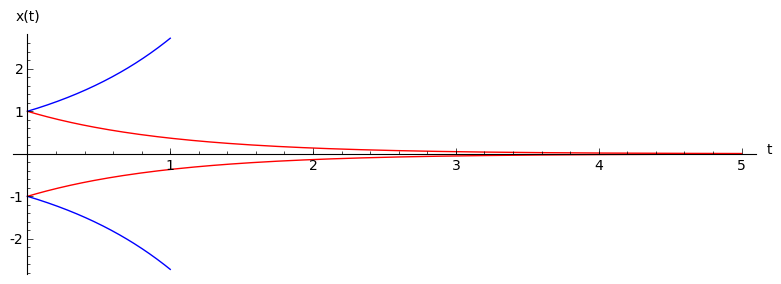
\includegraphics{sage_chI023_01.png}
\caption{Stabilość punktów stacjonarnych}\end{figure}

Na rysunku przedstawiono zagadnienie stabilności:  czerwone krzywe dążą do 0 gdy $t\to \infty$. Niebieskie  krzywe rozbiegają się (uciekają od   0) gdy $t\to \infty$.

Warunki początkowe $x(0)=\pm 0.05$ są blisko stanu stacjonarnego $x_s=0$. Przykład ten sugeruje nam metodę badania stabilności stanu stacjonarnego. Teraz podamy tę metodę.


\subsection{Metoda linearyzacji badania stabilności}
\label{ch1/chI023:metoda-linearyzacji-badania-stabilnosci}
Rozpatrujemy układ 1-wymiarowy:
\phantomsection\label{ch1/chI023:equation-eqn10}\begin{gather}
\begin{split}\frac{dx}{dt} = \dot x = f(x), \quad \quad f(x_s) = 0\end{split}\label{ch1/chI023-eqn10}
\end{gather}
Aby zbadać stabilność stanu  $x_s$, analizujemy zaburzenie
\phantomsection\label{ch1/chI023:equation-eqn11}\begin{gather}
\begin{split}h(t) = x(t) - x_s,  \quad \quad  |h(0)| = |x(0) - x_s| < \delta\end{split}\label{ch1/chI023-eqn11}
\end{gather}
Funkcja $h(t)$ powinna być mała, gdy stan $x_s$ jest stabilny. Jak daleko jest rozwiązanie $x(t)$ od rozwiązania $x_s$. Zobaczmy, jakie równanie różniczkowe spełnia $h(t)$:
\phantomsection\label{ch1/chI023:equation-eqn12}\begin{gather}
\begin{split}\frac{dh}{dt} = \frac{d}{dt} [x(t) - x_s] = \frac{dx}{dt} = f(x) = f( x_s +h)  = f(x_s) + f'(x_s) h + \frac{1}{2} f''(x_s) h^2 + \frac{1}{3!} f'''(x_s) h^3+ ....\end{split}\label{ch1/chI023-eqn12}
\end{gather}
Ponieważ $f(x_s)=0$, otrzymujemy równanie różniczkowe dla odchylenia $h(t)$ od stanu stacjonarnego
\phantomsection\label{ch1/chI023:equation-eqn13}\begin{gather}
\begin{split}\frac{dh}{dt} =  f'(x_s) h + \frac{1}{2} f''(x_s) h^2 + \frac{1}{3!} f'''(x_s) h^3+ ....\end{split}\label{ch1/chI023-eqn13}
\end{gather}
Jeżeli $f'(x_s) \ne 0$, to pierwszy istotny wyraz w tym równaniu jest liniowy
względem $h$.  Wyrazy $h^2,  h^3$ i wyższych potęg są pomijalnie małe.
Jeżeli np. $h =10^{-2}$ to  $h^2 = 10^{-4},  h^3 = 10^{-6}$. Wówczas
$h^2,  h^3$ i wyższe potęgi $h$  można pominąć jako bardzo małe.
Otrzymujemy równanie różniczkowe liniowe
\phantomsection\label{ch1/chI023:equation-eqn14}\begin{gather}
\begin{split}\frac{dh}{dt} =\lambda h, \quad \quad \lambda = f'(x_s)\end{split}\label{ch1/chI023-eqn14}
\end{gather}
z rozwiązaniem
\phantomsection\label{ch1/chI023:equation-eqn15}\begin{gather}
\begin{split}h(t) = h(0)  e^{\lambda t}\end{split}\label{ch1/chI023-eqn15}
\end{gather}
Wiemy już z powyższego przykładu, że gdy $\lambda < 0$ to $h(t) \to 0$ gdy $t\to \infty$. To oznacza, że  zaburzenie $x(t) \to x_s$ gdy  $t \to \infty$  i wówczas stan stacjonarny $x_s$ jest stabilny.  Jeżeli  $\lambda > 0$ to $|h(t)| \to \infty$ gdy $t\to \infty$. To oznacza, że  zaburzenie x(t) ucieka od $x_s$ gdy  $t \to \infty$  i wówczas stan stacjonarny $x_s$ jest niestabilny. Otrzymujemy następujące kryterium na stabilność stanu stacjonarnego:
\begin{itemize}
\item {} 
Jeżeli $\lambda = f'(x_s) < 0$ to  stan stacjonarny jest stabilny,

\item {} 
jeżeli $\lambda = f'(x_s) > 0$ to  stan stacjonarny jest niestabilny,

\item {} 
jeżeli $\lambda = f'(x_s) = 0$ to  nie wiem nic na temat stabilności. Musimy badać następne niezerowe wyrazy.  Jeżeli $f''(x_s) \ne 0$ zatrzymujemy pierwszy nieznikający wyraz czyli  badamy równanie
\phantomsection\label{ch1/chI023:equation-eqn16}\begin{gather}
\begin{split}\frac{dh}{dt} =\gamma h^2, \quad \quad \gamma  =  \frac{1}{2}f''(x_s)\end{split}\label{ch1/chI023-eqn16}
\end{gather}
Jeżeli  $f'(x_s) =0$ oraz $f''(x_s) =0$ to  bierzemy następny nieznikający wyraz i badamy równanie
\phantomsection\label{ch1/chI023:equation-eqn17}\begin{gather}
\begin{split} \frac{dh}{dt} =\nu h^3, \quad \quad \nu  =    \frac{1}{3!} f'''(x_s)\end{split}\label{ch1/chI023-eqn17}
\end{gather}
Jeżeli w tych przypadkach $h(t) \to 0$ gdy $t\to \infty$, to  stan stacjonarny $x_s$ jest stabilny. W przeciwnym przypadku  - nie jest stabilny.

\end{itemize}


\subsection{Metoda potencjału badania stabilności}
\label{ch1/chI023:metoda-potencjalu-badania-stabilnosci}
W jednym wymiarze, równanie różniczkowe  zawsze można przedstawić w postaci
\phantomsection\label{ch1/chI023:equation-eqn18}\begin{gather}
\begin{split}\frac{dx}{dt} = \dot x = f(x) = -\frac{dV(x)}{dx} = -V'(x), \quad \quad f(x_s) = 0\end{split}\label{ch1/chI023-eqn18}
\end{gather}
gdzie funkcja
\phantomsection\label{ch1/chI023:equation-eqn19}\begin{gather}
\begin{split}V(x) = -\int f(x)  dx\end{split}\label{ch1/chI023-eqn19}
\end{gather}
nazywana jest ``potencjałem''.  W ogólności to nie jest potencjał fizyczny który pojawia się w równaniu Newtona  dla cząstki z tłumieniem:
\phantomsection\label{ch1/chI023:equation-eqn20}\begin{gather}
\begin{split}m \ddot x + \gamma \dot x = -V'(x)\end{split}\label{ch1/chI023-eqn20}
\end{gather}
Jeżeli ruch cząstki odbywa się w środowisku o dużym  tarciu, w tzw. reżimie przetłumionym, w którym przyśpieszenie cząstki jest znikomo małe (formalnie gdy $m=0$), wówczas równanie Newtona ma postać
\phantomsection\label{ch1/chI023:equation-eqn21}\begin{gather}
\begin{split}\gamma \dot x = -V'(x)\end{split}\label{ch1/chI023-eqn21}
\end{gather}
które po przeskalowaniu ma postać:
\phantomsection\label{ch1/chI023:equation-eqn22}\begin{gather}
\begin{split}\dot x = -\frac{1}{\gamma} V'(x) = - {\tilde V} '(x)\end{split}\label{ch1/chI023-eqn22}
\end{gather}
Stąd też ``historycznie'' wywodzi sią nazwa potencjał dla abstrakcyjnego układu dynamicznego:
\phantomsection\label{ch1/chI023:equation-eqn23}\begin{gather}
\begin{split} \dot x = f(x) =  = -V'(x)\end{split}\label{ch1/chI023-eqn23}
\end{gather}
Stan stacjonarny $x_s$ określony równaniem
\phantomsection\label{ch1/chI023:equation-eqn24}\begin{gather}
\begin{split}f(x_s) = -V'(x_s) = 0\end{split}\label{ch1/chI023-eqn24}
\end{gather}
to punkt ekstremalny potencjału (o ile  pochodna parzystego rzędu $V^{(2k)}(x_s) \ne 0$).  Punkt $x_s$ jest stabilny gdy
\phantomsection\label{ch1/chI023:equation-eqn25}\begin{gather}
\begin{split}\lambda = f'(x_s) = - V''(x_s) < 0\end{split}\label{ch1/chI023-eqn25}
\end{gather}
czyli $V''(x_s) > 0$. To odpowiada minimum potencjału. Natomiast punkt $x_s$  niestabily odpowiada maksimum potencjału. Mamy więc klarowny obraz: Rysujemy potencjał $V(x)$. Minima potencjału to stabilne stany stacjonarne; maksima potencjału to niestabilne stany stacjonarne.
\setbox0\vbox{
\begin{minipage}{0.95\linewidth}
\textbf{Zadania}

\medskip


Wyznacz stany stacjonarne i zbadaj ich (asymptotyczną) stabilność. Korzystaj z metody linearyzacji i metody potencjału.
\begin{enumerate}
\item {} 
$\dot x = 4 x - x^3$

\item {} 
$\dot x = 1+x^4$

\item {} 
$\dot x =3 \sin(x)$

\item {} 
$\dot x =2x \sin(x)$

\item {} 
$\dot x =-x^2 \sin(x)$

\end{enumerate}
\end{minipage}}
\begin{center}\setlength{\fboxsep}{5pt}\shadowbox{\box0}\end{center}

Poniżej pokazujemy wyniki dla zadania 1. Są 3 stany stacjonarne:
$x_{s1} = 2,  x_{s2} = 0,  x_{s3} = -2$. Stany  $x_{s1} = 2$
oraz  $x_{s3} = -2$  są asymptotycznie stabilne (rozwiązania dążą
do tych stanów). Stan $x_{s2} = 0$  jest niestabilny (rozwiązania
uciekają od tego stanu).

\begin{Verbatim}[commandchars=\\\{\}]
\PYG{n}{var}\PYG{p}{(}\PYG{l+s}{\PYGZsq{}}\PYG{l+s}{x,y,z,u,Z,Y,t}\PYG{l+s}{\PYGZsq{}}\PYG{p}{)}
\PYG{n}{T0} \PYG{o}{=} \PYG{n}{srange}\PYG{p}{(}\PYG{l+m+mi}{0}\PYG{p}{,}\PYG{l+m+mf}{1.5}\PYG{p}{,}\PYG{l+m+mf}{0.01}\PYG{p}{)}
\PYG{n}{f11} \PYG{o}{=} \PYG{l+m+mi}{4}\PYG{o}{*}\PYG{n}{x}\PYG{o}{\PYGZhy{}}\PYG{n}{x}\PYG{o}{\PYGZca{}}\PYG{l+m+mi}{3}
\PYG{n}{f12} \PYG{o}{=} \PYG{l+m+mi}{4}\PYG{o}{*}\PYG{n}{y}\PYG{o}{\PYGZhy{}}\PYG{n}{y}\PYG{o}{\PYGZca{}}\PYG{l+m+mi}{3}
\PYG{n}{f13} \PYG{o}{=} \PYG{l+m+mi}{4}\PYG{o}{*}\PYG{n}{z}\PYG{o}{\PYGZhy{}}\PYG{n}{z}\PYG{o}{\PYGZca{}}\PYG{l+m+mi}{3}
\PYG{n}{f15} \PYG{o}{=} \PYG{l+m+mi}{4}\PYG{o}{*}\PYG{n}{u}\PYG{o}{\PYGZhy{}}\PYG{n}{u}\PYG{o}{\PYGZca{}}\PYG{l+m+mi}{3}
\PYG{n}{f16} \PYG{o}{=} \PYG{l+m+mi}{0}
\PYG{n}{de} \PYG{o}{=} \PYG{n}{vector}\PYG{p}{(}\PYG{p}{[}\PYG{n}{f11}\PYG{p}{,}\PYG{n}{f12}\PYG{p}{,}\PYG{n}{f13}\PYG{p}{,}\PYG{l+m+mi}{0}\PYG{p}{,}\PYG{l+m+mi}{0}\PYG{p}{,}\PYG{n}{f15}\PYG{p}{]}\PYG{p}{)}
\PYG{n}{ic} \PYG{o}{=} \PYG{p}{[}\PYG{l+m+mi}{4}\PYG{p}{,}\PYG{l+m+mf}{0.2}\PYG{p}{,}\PYG{o}{\PYGZhy{}}\PYG{l+m+mf}{0.2}\PYG{p}{,}\PYG{l+m+mi}{2}\PYG{p}{,}\PYG{o}{\PYGZhy{}}\PYG{l+m+mi}{2}\PYG{p}{,}\PYG{o}{\PYGZhy{}}\PYG{l+m+mi}{4}\PYG{p}{]}
\PYG{n}{sol5}\PYG{o}{=}\PYG{n}{desolve\PYGZus{}odeint}\PYG{p}{(}\PYG{n}{de}\PYG{p}{,}\PYG{n}{ic}\PYG{p}{,}\PYG{n}{T0}\PYG{p}{,}\PYG{p}{[}\PYG{n}{x}\PYG{p}{,}\PYG{n}{y}\PYG{p}{,}\PYG{n}{z}\PYG{p}{,}\PYG{n}{Z}\PYG{p}{,}\PYG{n}{Y}\PYG{p}{,}\PYG{n}{u}\PYG{p}{]}\PYG{p}{)}
\PYG{n}{line}\PYG{p}{(}\PYG{n+nb}{zip}\PYG{p}{(}\PYG{n}{T0}\PYG{p}{,}\PYG{n}{sol5}\PYG{p}{[}\PYG{p}{:}\PYG{p}{,}\PYG{l+m+mi}{0}\PYG{p}{]}\PYG{p}{)}\PYG{p}{,}\PYG{n}{figsize}\PYG{o}{=}\PYG{p}{(}\PYG{l+m+mi}{7}\PYG{p}{,} \PYG{l+m+mi}{4}\PYG{p}{)}\PYG{p}{)}\PYG{o}{+}\PYGZbs{}
 \PYG{n}{line}\PYG{p}{(}\PYG{n+nb}{zip}\PYG{p}{(}\PYG{n}{T0}\PYG{p}{,}\PYG{n}{sol5}\PYG{p}{[}\PYG{p}{:}\PYG{p}{,}\PYG{l+m+mi}{1}\PYG{p}{]}\PYG{p}{)}\PYG{p}{,}\PYG{n}{color}\PYG{o}{=}\PYG{l+s}{\PYGZsq{}}\PYG{l+s}{red}\PYG{l+s}{\PYGZsq{}}\PYG{p}{)}\PYG{o}{+}\PYGZbs{}
 \PYG{n}{line}\PYG{p}{(}\PYG{n+nb}{zip}\PYG{p}{(}\PYG{n}{T0}\PYG{p}{,}\PYG{n}{sol5}\PYG{p}{[}\PYG{p}{:}\PYG{p}{,}\PYG{l+m+mi}{2}\PYG{p}{]}\PYG{p}{)}\PYG{p}{,}\PYG{n}{color}\PYG{o}{=}\PYG{l+s}{\PYGZsq{}}\PYG{l+s}{green}\PYG{l+s}{\PYGZsq{}}\PYG{p}{)}\PYG{o}{+}\PYGZbs{}
 \PYG{n}{line}\PYG{p}{(}\PYG{n+nb}{zip}\PYG{p}{(}\PYG{n}{T0}\PYG{p}{,}\PYG{n}{sol5}\PYG{p}{[}\PYG{p}{:}\PYG{p}{,}\PYG{l+m+mi}{4}\PYG{p}{]}\PYG{p}{)}\PYG{p}{,}\PYG{n}{color}\PYG{o}{=}\PYG{l+s}{\PYGZsq{}}\PYG{l+s}{gray}\PYG{l+s}{\PYGZsq{}}\PYG{p}{)}\PYG{o}{+}\PYGZbs{}
 \PYG{n}{line}\PYG{p}{(}\PYG{n+nb}{zip}\PYG{p}{(}\PYG{n}{T0}\PYG{p}{,}\PYG{n}{sol5}\PYG{p}{[}\PYG{p}{:}\PYG{p}{,}\PYG{l+m+mi}{5}\PYG{p}{]}\PYG{p}{)}\PYG{p}{,}\PYG{n}{color}\PYG{o}{=}\PYG{l+s}{\PYGZsq{}}\PYG{l+s}{black}\PYG{l+s}{\PYGZsq{}}\PYG{p}{)}\PYG{o}{+}\PYGZbs{}
 \PYG{n}{line}\PYG{p}{(}\PYG{n+nb}{zip}\PYG{p}{(}\PYG{n}{T0}\PYG{p}{,}\PYG{n}{sol5}\PYG{p}{[}\PYG{p}{:}\PYG{p}{,}\PYG{l+m+mi}{3}\PYG{p}{]}\PYG{p}{)}\PYG{p}{,}\PYG{n}{color}\PYG{o}{=}\PYG{l+s}{\PYGZsq{}}\PYG{l+s}{violet}\PYG{l+s}{\PYGZsq{}}\PYG{p}{)}
\end{Verbatim}
\begin{figure}[htbp]
\centering
\capstart

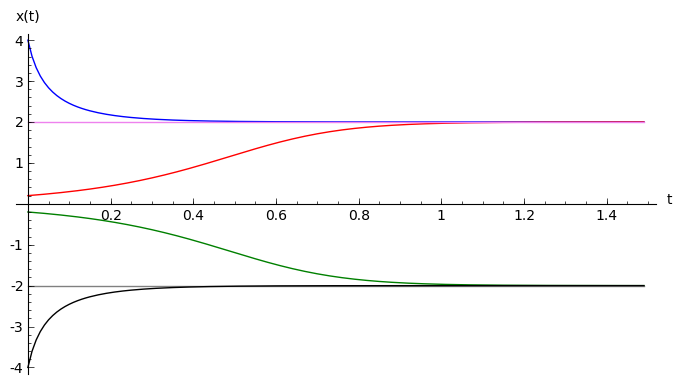
\includegraphics{sage_chI023_02.png}
\caption{Stabilość punktów stacjonarnych}\end{figure}

Z powyższego przykładu zauważmy następujące cechy:
\begin{enumerate}
\item {} 
Zbiór warunków początkowych dzieli się na dwa podzbiory $A_1 = (-\infty, 0)$ oraz  $A_2=(0, \infty)$. Dla warunków  początkowych ze zbioru $A_1$ rozwiązania $x(t) \to -2$ dla $t\to\infty$, a  dla warunków  początkowych ze zbioru $A_2$ rozwiązania $x(t) \to 2$ dla $t\to\infty$.

\item {} 
Krzywe $x(t)$  są funkcjami monotonicznymi: albo cały czas rosną w czasie, albo cały czas maleją gdy czas rośnie. Dlaczego? Rozważmy  2 przykłady warunków początkowych widocznych na rysunku:

\end{enumerate}
\begin{enumerate}
\item {} 
gdy $x(0) = 4$ to $\dot x (x=4) = 4\cdot 4 -4^3 = -48 < 0$.   Pochodna jest ujemna, a to oznacza że funkcja maleje. Podobnie jest dla wszystkich warunków początkowych $x(0) > 2$

\item {} 
gdy $x(0) = 0.2$ to $\dot x (x=0.2) = 4\cdot 0.2 -(0.2)^3 > 0$.  Pochodna jest dodatnia, a to oznacza że funkcja rośnie. Podobnie jest dla wszystkich warunków początkowych $x(0)  \in (0, 2)$

\end{enumerate}
\begin{enumerate}
\setcounter{enumi}{2}
\item {} 
Różne krzywe $x(t)$ nigdy się nie przecinają. Wynika to z tego, że rozwiązania są jedyne i jednoznaczne. Jeżeli by się przecinały,  to z punktu przecięcia wychodziłoby kilka rozwiązań. A to jest niemożliwe na mocy twierdzenia o jednoznaczności rozwiązań.

\end{enumerate}


\subsection{Przypadek B: Układ  2 równań różniczkowych}
\label{ch1/chI023:przypadek-b-uklad-2-rownan-rozniczkowych}
Dla jasności prezentacji, rozpatrujemy układ 2 równań różniczkowych
\phantomsection\label{ch1/chI023:equation-eqn26}\begin{gather}
\begin{split}\dot x = f(x, y),\end{split}\label{ch1/chI023-eqn26}\\\begin{split}\dot y = g(x, y).\end{split}\notag
\end{gather}
Stany stacjonarne $(x_s, y_s)$  określone są jako rozwiązania układu równań algebraicznych
\phantomsection\label{ch1/chI023:equation-eqn27}\begin{gather}
\begin{split}f(x_s, y_s)=0,\end{split}\label{ch1/chI023-eqn27}\\\begin{split}g(x_s, y_s) =0.\end{split}\notag
\end{gather}
Gdyby istniał potencjał $V(x, y)$, powyżej przedstawione wnioski otrzymane z metody potencjału są  także prawdziwe dla układów wielowymiarowych. Ponieważ w ogólnym  przypadku ``potencjał'' nie musi istnieć,  zbadamy  stabilność stanów   $(x_s, y_s)$  stosując metodę linearyzacji. Definiujemy  nowe funkcje
\phantomsection\label{ch1/chI023:equation-eqn28}\begin{gather}
\begin{split}X(t) = x(t) - x_s,\end{split}\label{ch1/chI023-eqn28}\\\begin{split}Y(t)=y(t)-y_s.\end{split}\notag
\end{gather}
Charakteryzują one odchylenie od stanu stacjonarnego, które są małe gdy stan stacjonarny jest stabilny. Zobaczymy, jakie równania różniczkowe spełniają te funkcje:
\phantomsection\label{ch1/chI023:equation-eqn29}\begin{gather}
\begin{split}\dot X(t) = \dot x(t) - \dot x_s  = \dot x(t) =  f(x(t), y(t)) = f(x_s +X(t), y_s + Y(t))  = f(x_s, y_s) + \frac{\partial f}{\partial x}  X + \frac{\partial f}{\partial y} Y+ ...\end{split}\label{ch1/chI023-eqn29}
\end{gather}\phantomsection\label{ch1/chI023:equation-eqn30}\begin{gather}
\begin{split} \dot Y(t)= \dot y(t) - \dot y_s  = \dot y(t) =  g(x(t), y(t)) =g(x_s +X(t), y_s + Y(t))  = gf(x_s, y_s) + \frac{\partial g}{\partial x}  X + \frac{\partial g}{\partial y} Y + ...\end{split}\label{ch1/chI023-eqn30}
\end{gather}
Wszystkie pochodne cząstkowe są obliczane w punkcie $(x_s, y_s)$. Ponieważ w punkcie stacjonarnym $f(x_s, y_s)=g(x_s, y_s)=0$ otrzymujemy zlinearyzowane równania różniczkowe w postaci
\phantomsection\label{ch1/chI023:equation-eqn31}\begin{gather}
\begin{split}\dot X =  a_{11} X +  a_{12} Y\end{split}\label{ch1/chI023-eqn31}
\end{gather}\phantomsection\label{ch1/chI023:equation-eqn32}\begin{gather}
\begin{split} \dot Y=  a_{21} X +  a_{22} Y\end{split}\label{ch1/chI023-eqn32}
\end{gather}
gdzie macierz współczynników
\phantomsection\label{ch1/chI023:equation-eqn33}\begin{gather}
\begin{split} \qquad \quad J = \begin{bmatrix}\frac{ \partial f}{\partial x}& \frac{\partial f}{\partial y}\\ \frac{\partial g}{\partial x}& \frac{\partial g}{\partial y}  \end{bmatrix}  =   \begin{bmatrix}a_{11} &  a_{12} \\ a_{21}& a_{22}  \end{bmatrix}   \quad \quad \mbox{obliczona w punkcie} \quad (x_s, y_s)\end{split}\label{ch1/chI023-eqn33}
\end{gather}
jest macierzą Jacobiego. Ponieważ otrzymaliśmy liniowy układ równań różniczkowych,  jego rozwiązania poszukujemy w postaci funkcji
\phantomsection\label{ch1/chI023:equation-eqn34}\begin{gather}
\begin{split}X(t) = A e^{\lambda t}, \quad \quad  Y(t) = B e^{\lambda t}\end{split}\label{ch1/chI023-eqn34}
\end{gather}
gdzie stałe $A$ oraz $B$ są określone przez warunki początkowe $(X(0), Y(0))$.

Zauważamy, że
\phantomsection\label{ch1/chI023:equation-eqn35}\begin{gather}
\begin{split} \dot X = \lambda X, \quad \quad \dot Y = \lambda  Y\end{split}\label{ch1/chI023-eqn35}
\end{gather}
Wstawiamy te relacje do  układu równań zlinearyzowanych:
\phantomsection\label{ch1/chI023:equation-eqn36}\begin{gather}
\begin{split}\lambda A = a_{11} A +  a_{12} B\end{split}\label{ch1/chI023-eqn36}
\end{gather}\phantomsection\label{ch1/chI023:equation-eqn37}\begin{gather}
\begin{split} \lambda  Y=  a_{21} A +  a_{22} B\end{split}\label{ch1/chI023-eqn37}
\end{gather}
Jest to zagadnienie własne dla macierzy Jacobiego, gdzie $\lambda$ to są wartości własne macierzy Jacobiego. To   jest także  równoważne liniowemu układowi równań algebraicznych
\phantomsection\label{ch1/chI023:equation-eqn38}\begin{gather}
\begin{split}\ (a_{11} - \lambda) A +  a_{12} B  = 0\end{split}\label{ch1/chI023-eqn38}
\end{gather}\phantomsection\label{ch1/chI023:equation-eqn39}\begin{gather}
\begin{split}a_{21} A +  (a_{22} -\lambda) B  = 0\end{split}\label{ch1/chI023-eqn39}
\end{gather}
Taki układ ma niezerowe rozwiązanie dla $A$ oraz $B$ gdy wyznacznik
\phantomsection\label{ch1/chI023:equation-eqn40}\begin{gather}
\begin{split}\det (J-\lambda I) = \left| \begin{array}{cc} a_{11} -\lambda &  a_{12} \\ a_{21}& a_{22} - \lambda  \end{array} \right| = (a_{11} -\lambda) ( a_{22} -\lambda) -a_{12} a_{21} = \lambda^2  - (a_{11} +a_{22} ) \lambda +a_{11} a_{22} -a_{12} a_{21} = 0\end{split}\label{ch1/chI023-eqn40}
\end{gather}
Macierz $I$ jest macierzą jednostkową, tzn. diagonalną $2\times 2$ i wszystkie elementy diagonalne to 1. Z powyższej relacji  otrzymujemy równanie kwadratowe dla nieznanych wartości  własnych $\lambda = \lambda_1$  oraz $\lambda = \lambda_2$.

Rozwiązanie zlinearyzowanego układu jest w postaci kombinacji liniowej :
\phantomsection\label{ch1/chI023:equation-eqn41}\begin{gather}
\begin{split}X(t) = A_1  e^{\lambda_1 t} + A_2 e^{\lambda_2 t}, \quad \quad  Y(t) = B_1 e^{\lambda_1 t} +  B_2 e^{\lambda_2 t}\end{split}\label{ch1/chI023-eqn41}
\end{gather}
Pytanie o stabilność stanu stacjonarnego $(x_s, y_s)$ jest równoważne pytaniu: kiedy
\phantomsection\label{ch1/chI023:equation-eqn42}\begin{gather}
\begin{split}\lim_{t\to \infty} X(t) = 0  \quad \quad \lim_{t\to \infty} Y(t) = 0\end{split}\label{ch1/chI023-eqn42}
\end{gather}
Funkcje exponencjalne dążą do zera jeżeli część rzeczywista  wartości własnych macierzy Jacobiego $\lambda_i$ są  ujemne:
\phantomsection\label{ch1/chI023:equation-eqn43}\begin{gather}
\begin{split} Re(\lambda_1) < 0, \quad \quad Re(\lambda_2) < 0\end{split}\label{ch1/chI023-eqn43}
\end{gather}
Wówczas stan stacjonarny jest asymptotycznie stabilny. Jeżeli
\phantomsection\label{ch1/chI023:equation-eqn44}\begin{gather}
\begin{split} Re(\lambda_1) > 0, \quad \quad \mbox{i/lub} \quad \quad Re(\lambda_2) >  0\end{split}\label{ch1/chI023-eqn44}
\end{gather}
to stan stacjonarny jest niestabilny. Jeżeli
\phantomsection\label{ch1/chI023:equation-eqn45}\begin{gather}
\begin{split} Re(\lambda_1) = Re(\lambda_2) =  0\end{split}\label{ch1/chI023-eqn45}
\end{gather}
to stan stacjonarny jest stabilny, ale nie  jest asymptotycznie stabilny. Jeżeli wartości własne macierzy Jacobiego wynoszą zero, metoda linearyzacji nie rozstrzyga o stabilności.

Zamiast wyznaczyć wartości własne $(\lambda_{1}, \lambda_{2})$ tej macierzy, wystarczy sprawdzić, kiedy część rzeczywista wartości własnych jest ujemna (lub dodatnia).  Ponieważ macierz Jacobiego jest macierzą $2 \times 2$, więc otrzymujemy równanie kwadratowe  dla $\lambda$. Aby wartości własne miały część rzeczywistą ujemną muszą zachodzić dwie relacje:
\phantomsection\label{ch1/chI023:equation-eqn46}\begin{gather}
\begin{split}\lambda_1 + \lambda_2  = a_{11}  + a_{22} <0  \quad \mbox{oraz} \quad \lambda_1 \; \lambda_2 = a_{11} a_{22}  -a_{12}a_{21} > 0,\end{split}\label{ch1/chI023-eqn46}
\end{gather}
to oznacza że
\phantomsection\label{ch1/chI023:equation-eqn46a}\begin{gather}
\begin{split}\mbox{Tr} \, J < 0, \quad \quad \det \,J > 0\end{split}\label{ch1/chI023-eqn46a}
\end{gather}
gdzie Tr oznacza ślad macierzy, czyli sumę elementów diagonalnych macierzy oraz $\det$ jest wyznacznikiem macierzy.


\subsubsection{Przykład 1}
\label{ch1/chI023:przyklad-1}
Rozważmy układ równań różniczkowych
\phantomsection\label{ch1/chI023:equation-eqn47}\begin{gather}
\begin{split}\dot x= 1-xy = f(x, y),\end{split}\label{ch1/chI023-eqn47}\\\begin{split}\dot y = x-y^2 = g(x, y).\end{split}\notag
\end{gather}
Łatwo znaleźć stany stacjonarne
\phantomsection\label{ch1/chI023:equation-eqn48}\begin{gather}
\begin{split} 1-xy = 0,\end{split}\label{ch1/chI023-eqn48}\\\begin{split} x-y^2 = 0.\end{split}\notag
\end{gather}
Z drugiego równania $x=y^2$ wstawiamy do pierwszego równania: $1-y^3=0$ czyli $y^3=1$. Stąd $y=1$ oraz $x=1$. Otrzymujemy stan stacjonarny
\phantomsection\label{ch1/chI023:equation-eqn49}\begin{gather}
\begin{split}(x_s, y_s) = (1, 1)\end{split}\label{ch1/chI023-eqn49}
\end{gather}
Obliczmy elementy macierzy Jacobiego
\phantomsection\label{ch1/chI023:equation-eqn50}\begin{gather}
\begin{split} \qquad \quad J = \begin{bmatrix}\frac{ \partial f}{\partial x}& \frac{\partial f}{\partial y}\\ \frac{\partial g}{\partial x}& \frac{\partial g}{\partial y}  \end{bmatrix}  =   \begin{bmatrix}-y & -x \\ 1& -2y  \end{bmatrix}    =  \begin{bmatrix}-1 & -1 \\ 1& -2  \end{bmatrix}\quad \quad \mbox{w punkcie} \quad (x=1, y=1)\end{split}\label{ch1/chI023-eqn50}
\end{gather}
Ślad macierz $J$, czyli suma elementów diagonalnych $\mbox{Tr} J = -3 < 0$ oraz wyznacznik $\det(J) = 3 > 0$. Spełnione są relacje dla stany stacjonarnego który jest asymptotycznie stabilny. Wniosek: stan stacjonarny $(x_s, y_s) = (1, 1)$ jest asymptotycznie stabilny.

Można sprawdzić to, wyliczając explicite wartości własne macierzy Jacobiego:
\phantomsection\label{ch1/chI023:equation-eqn51}\begin{gather}
\begin{split}\lambda_1 = \frac{1}{2} (-3+i \sqrt 3), \quad \quad \lambda_1 = \frac{1}{2} (-3-i \sqrt 3)\end{split}\label{ch1/chI023-eqn51}
\end{gather}
Ich części rzeczywiste są ujemne:  $\Re(\lambda_1) = -3/2,  \Re(\lambda_2) = -3/2$.


\subsection{Przypadek C: Stabilność stanów stacjonarnych układów wielowymiarowych}
\label{ch1/chI023:przypadek-c-stabilnosc-stanow-stacjonarnych-ukladow-wielowymiarowych}
Dla układu równań różniczkowych o wymiarze większym niż 2 stosujemy te same metody co dla układu 2 równań różniczkowych.  Oczywiście istnieje więcej różnych przypadków i większe bogactwo własności  stanów stacjonarnych.  Nie będziemy przedstawiali tu przypadku o dowolnym wymiarze. Rozważymy przypadek 3 równań, aby pokazać podobieństwo do przypadku 2 równań. Analizujemy układ 3 równań różniczkowych:
\phantomsection\label{ch1/chI023:equation-eqn52}\begin{gather}
\begin{split}\dot x = F_1(x, y, z), \quad x(0) = x_0,\end{split}\label{ch1/chI023-eqn52}\\\begin{split}\dot y = F_2(x, y, z),  \quad y(0) = y_0,\end{split}\notag\\\begin{split}\dot z = F_3(x, y, z),  \quad z(0) = z_0.\end{split}\notag
\end{gather}
Stany stacjonarne są określone przez rozwiązania układu równań algebraicznych:
\phantomsection\label{ch1/chI023:equation-eqn53}\begin{gather}
\begin{split}F_1(x, y, z) = 0, \quad  F_2(x, y, z) = 0,  \quad  F_3(x, y, z)=0\end{split}\label{ch1/chI023-eqn53}
\end{gather}
Z równań tych otrzymujemy  stan stacjonarny   $(x, y, z,) = (x_{s}, y_{s}, z_s)$. Następnie obliczmy macierz Jacobiego
\phantomsection\label{ch1/chI023:equation-eqn54}\begin{gather}
\begin{split} J = \begin{bmatrix}\frac{ \partial F_1}{\partial x}& \frac{\partial F_1}{\partial y}&\frac{ \partial F_1}{\partial z}\\ \frac{ \partial F_2}{\partial x}&  \frac{ \partial F_2}{\partial y} &\frac{ \partial F_2}{\partial z} \\ \frac{ \partial F_3}{\partial x}& \frac{ \partial F_3}{\partial y}&\frac{ \partial F_3}{\partial z} \end{bmatrix}\end{split}\label{ch1/chI023-eqn54}
\end{gather}
Obliczmy  macierz Jacobiego w punkcie stacjonarnym $J=J(x_s, y_s, z_s)$.  W ten sposób otrzymujemy macierz liczbową. Kolejnym krokiem jest znalezienie wartości własnych $\lambda = \lambda_i   (i=1, 2, 3)$   tej macierzy, czyli rozwiązanie  wielomianu 3-go stopnia dla $\lambda$:
\phantomsection\label{ch1/chI023:equation-eqn55}\begin{gather}
\begin{split} \det (J -\lambda I)  = \left| \begin{array}{ccc}\frac{ \partial F_1}{\partial x} -\lambda & \frac{\partial F_1}{\partial y}&\frac{ \partial F_1}{\partial z}\\ \frac{ \partial F_2}{\partial x}&  \frac{ \partial F_2}{\partial y} -\lambda &\frac{ \partial F_2}{\partial z} \\ \frac{ \partial F_3}{\partial x}& \frac{ \partial F_3}{\partial y}&\frac{ \partial F_3}{\partial z} -\lambda \end{array} \right| =  0\end{split}\label{ch1/chI023-eqn55}
\end{gather}
Macierz $I$ jest macierzą jednostkową, tzn. diagonalną $3\times 3$ i wszystkie elementy diagonalne to 1.

Jeżeli części  rzeczywiste  wszystkich wartości własnych macierzy Jacobiego $\lambda_i$ są  ujemne:
\phantomsection\label{ch1/chI023:equation-eqn56}\begin{gather}
\begin{split} \Re(\lambda_1) < 0, \quad \quad \Re(\lambda_2) < 0, \quad \quad \Re(\lambda_3) < 0\end{split}\label{ch1/chI023-eqn56}
\end{gather}
to  stan stacjonarny jest asymptotycznie stabilny. Jeżeli  chociaż jedna z wartości własnych $\lambda_i$ ma część rzeczywistą dodatnią
\phantomsection\label{ch1/chI023:equation-eqn57}\begin{gather}
\begin{split} \Re(\lambda_1) > 0, \quad \quad \mbox{i/lub} \quad \quad \Re(\lambda_2) >  0, \quad \quad \mbox{i/lub} \quad \quad \Re(\lambda_3) >  0\end{split}\label{ch1/chI023-eqn57}
\end{gather}
to stan stacjonarny jest niestabilny.

W przypadkach wielowymiarowych wygodnie jest stosować metody numeryczne. Obliczanie wartości własnych macierzy jest numerycznie zadaniem łatwym.


\subsubsection{Przykład 2: Model Lorenza}
\label{ch1/chI023:przyklad-2-model-lorenza}\phantomsection\label{ch1/chI023:equation-eqn58}\begin{gather}
\begin{split}\dot x = \sigma (y-x) = F_1(x, y,  z), \qquad x(0) = x_0,\end{split}\label{ch1/chI023-eqn58}\\\begin{split}\dot y = x(\rho - z) -y = F_2(x, y,  z), \qquad y(0) = y_0,\end{split}\notag\\\begin{split}\dot z = x y - \beta z = F_3(x, y,  z), \qquad z(0) = z_0.\end{split}\notag
\end{gather}
gdzie wszystkie parametry są dodatnie: $\sigma, \rho, \beta > 0$.

Znajdujemy stany stacjonarne czyli rozwiązujemy układ równań algebraicznych
\phantomsection\label{ch1/chI023:equation-eqn59}\begin{gather}
\begin{split}\sigma (y-x) =0,\end{split}\label{ch1/chI023-eqn59}\\\begin{split}x(\rho - z) -y = 0,\end{split}\notag\\\begin{split}x y - \beta z = 0.\end{split}\notag
\end{gather}
Możemy posłużyć się programem w Sage, ale układ ten jest na tyle prosty, że możemy go rozwiązać  sami. Z pierwszego równania wynika, że
\phantomsection\label{ch1/chI023:equation-eqn60}\begin{gather}
\begin{split}y=x,\end{split}\label{ch1/chI023-eqn60}
\end{gather}
z trzeciego równania otrzymujemy
\phantomsection\label{ch1/chI023:equation-eqn61}\begin{gather}
\begin{split}z= \frac{1}{\beta} x^2.\end{split}\label{ch1/chI023-eqn61}
\end{gather}
Teraz wstawiamy $x$ oraz $z$ do drugiego równania otrzymując relację:
\phantomsection\label{ch1/chI023:equation-eqn62}\begin{gather}
\begin{split}x \rho - x   {\frac{1}{\beta} }x^2 -x=0,\end{split}\label{ch1/chI023-eqn62}
\end{gather}
czyli
\phantomsection\label{ch1/chI023:equation-eqn63}\begin{gather}
\begin{split}x [ \rho - 1  - {\frac{1}{\beta} }x^2]=0.\end{split}\label{ch1/chI023-eqn63}
\end{gather}
Ta relacja jest prosta i wynika z niej że
\phantomsection\label{ch1/chI023:equation-eqn64}\begin{gather}
\begin{split}x= x_1 = 0 \quad \mbox{lub} \quad x=  x_2 = \sqrt{\beta ( \rho -1)} \quad \mbox{lub} \quad x= x_3 =  - \sqrt{\beta ( \rho -1)}\end{split}\label{ch1/chI023-eqn64}
\end{gather}
Otrzymujemy 3 stany stacjonarne:
\phantomsection\label{ch1/chI023:equation-eqn65}\begin{gather}
\begin{split}P_1 = (x_1, y_1, z_1) =  (0, 0, 0),\end{split}\label{ch1/chI023-eqn65}\\\begin{split}P_2 = (x_2, y_2, z_2) =  ( \sqrt{\beta ( \rho -1)}, \sqrt{\beta ( \rho -1)}, \rho - 1),\end{split}\notag\\\begin{split}P_3 = (x_3, y_3, z_3) =  ( - \sqrt{\beta ( \rho -1)}, -  \sqrt{\beta ( \rho -1)}, \rho - 1).\end{split}\notag
\end{gather}
Dla każdego stanu stacjonarnego musimy zbadać jego stabilność analizując zagadnienie własne dla macierzy Jacobiego. No to do dzieła...

\begin{Verbatim}[commandchars=\\\{\}]
\PYG{c}{\PYGZsh{}kilka zmiennych}
\PYG{n}{var}\PYG{p}{(}\PYG{l+s}{\PYGZsq{}}\PYG{l+s}{x y z sigma rho beta alpha}\PYG{l+s}{\PYGZsq{}}\PYG{p}{)}
\PYG{c}{\PYGZsh{}i kilka zalozen}
\PYG{n}{assume}\PYG{p}{(}\PYG{n}{sigma}\PYG{o}{\PYGZgt{}}\PYG{l+m+mi}{0}\PYG{p}{)}
\PYG{n}{assume}\PYG{p}{(}\PYG{n}{rho}\PYG{o}{\PYGZgt{}}\PYG{l+m+mi}{0}\PYG{p}{)}
\PYG{n}{assume}\PYG{p}{(}\PYG{n}{beta}\PYG{o}{\PYGZgt{}}\PYG{l+m+mi}{0}\PYG{p}{)}
\PYG{c}{\PYGZsh{}definiujemy rownania rozniczkowe}
\PYG{n}{F1} \PYG{o}{=} \PYG{n}{sigma}\PYG{o}{*}\PYG{p}{(}\PYG{n}{y}\PYG{o}{\PYGZhy{}}\PYG{n}{x}\PYG{p}{)}
\PYG{n}{F2} \PYG{o}{=} \PYG{n}{x}\PYG{o}{*}\PYG{p}{(}\PYG{n}{rho}\PYG{o}{\PYGZhy{}}\PYG{n}{z}\PYG{p}{)} \PYG{o}{\PYGZhy{}} \PYG{n}{y}
\PYG{n}{F3} \PYG{o}{=} \PYG{n}{x}\PYG{o}{*}\PYG{n}{y} \PYG{o}{\PYGZhy{}} \PYG{n}{beta}\PYG{o}{*}\PYG{n}{z}
\PYG{c}{\PYGZsh{}stany stacjonarne}
\PYG{n}{rozw} \PYG{o}{=} \PYG{n}{solve}\PYG{p}{(}\PYG{p}{[}\PYG{n}{F1}\PYG{o}{==}\PYG{l+m+mi}{0}\PYG{p}{,}\PYG{n}{F2}\PYG{o}{==}\PYG{l+m+mi}{0}\PYG{p}{,}\PYG{n}{F3}\PYG{o}{==}\PYG{l+m+mi}{0}\PYG{p}{]}\PYG{p}{,}\PYG{p}{[}\PYG{n}{x}\PYG{p}{,}\PYG{n}{y}\PYG{p}{,}\PYG{n}{z}\PYG{p}{]}\PYG{p}{)}
\PYG{n}{P1} \PYG{o}{=} \PYG{n}{rozw}\PYG{p}{[}\PYG{l+m+mi}{2}\PYG{p}{]}
\PYG{n}{P2} \PYG{o}{=} \PYG{n}{rozw}\PYG{p}{[}\PYG{l+m+mi}{0}\PYG{p}{]}
\PYG{n}{P3} \PYG{o}{=} \PYG{n}{rozw}\PYG{p}{[}\PYG{l+m+mi}{1}\PYG{p}{]}
\PYG{c}{\PYGZsh{}macierz Jakobiego}
\PYG{n}{J} \PYG{o}{=} \PYG{n}{matrix}\PYG{p}{(}\PYG{p}{[}
\PYG{p}{[}\PYG{n}{diff}\PYG{p}{(}\PYG{n}{F1}\PYG{p}{,}\PYG{n}{x}\PYG{p}{)}\PYG{p}{,}\PYG{n}{diff}\PYG{p}{(}\PYG{n}{F1}\PYG{p}{,}\PYG{n}{y}\PYG{p}{)}\PYG{p}{,}\PYG{n}{diff}\PYG{p}{(}\PYG{n}{F1}\PYG{p}{,}\PYG{n}{z}\PYG{p}{)}\PYG{p}{]}\PYG{p}{,}
\PYG{p}{[}\PYG{n}{diff}\PYG{p}{(}\PYG{n}{F2}\PYG{p}{,}\PYG{n}{x}\PYG{p}{)}\PYG{p}{,}\PYG{n}{diff}\PYG{p}{(}\PYG{n}{F2}\PYG{p}{,}\PYG{n}{y}\PYG{p}{)}\PYG{p}{,}\PYG{n}{diff}\PYG{p}{(}\PYG{n}{F2}\PYG{p}{,}\PYG{n}{z}\PYG{p}{)}\PYG{p}{]}\PYG{p}{,}
\PYG{p}{[}\PYG{n}{diff}\PYG{p}{(}\PYG{n}{F3}\PYG{p}{,}\PYG{n}{x}\PYG{p}{)}\PYG{p}{,}\PYG{n}{diff}\PYG{p}{(}\PYG{n}{F3}\PYG{p}{,}\PYG{n}{y}\PYG{p}{)}\PYG{p}{,}\PYG{n}{diff}\PYG{p}{(}\PYG{n}{F3}\PYG{p}{,}\PYG{n}{z}\PYG{p}{)}\PYG{p}{]}
\PYG{p}{]}\PYG{p}{)}
\PYG{c}{\PYGZsh{}analiza stabilnosci}
\PYG{n}{punkt}\PYG{o}{=}\PYG{l+s}{\PYGZsq{}}\PYG{l+s}{P1}\PYG{l+s}{\PYGZsq{}} \PYG{c}{\PYGZsh{} lub \PYGZsq{}P2\PYGZsq{},\PYGZsq{}P3\PYGZsq{}}
\PYG{c}{\PYGZsh{}\PYGZsh{}automatycznie}
\PYG{n}{P} \PYG{o}{=} \PYG{n+nb}{dict}\PYG{p}{(}\PYG{n+nb}{zip}\PYG{p}{(}\PYG{p}{[}\PYG{l+s}{\PYGZsq{}}\PYG{l+s}{P1}\PYG{l+s}{\PYGZsq{}}\PYG{p}{,}\PYG{l+s}{\PYGZsq{}}\PYG{l+s}{P2}\PYG{l+s}{\PYGZsq{}}\PYG{p}{,}\PYG{l+s}{\PYGZsq{}}\PYG{l+s}{P3}\PYG{l+s}{\PYGZsq{}}\PYG{p}{]}\PYG{p}{,}\PYG{p}{[}\PYG{n}{P1}\PYG{p}{,}\PYG{n}{P2}\PYG{p}{,}\PYG{n}{P3}\PYG{p}{]}\PYG{p}{)}\PYG{p}{)}\PYG{p}{[}\PYG{n}{punkt}\PYG{p}{]}
\PYG{n}{J} \PYG{o}{=} \PYG{n}{matrix}\PYG{p}{(}\PYG{p}{[}
\PYG{p}{[}
\PYG{n}{diff}\PYG{p}{(}\PYG{n}{F1}\PYG{p}{,}\PYG{n}{x}\PYG{p}{)}\PYG{p}{(}\PYG{n}{x}\PYG{o}{=}\PYG{n}{P}\PYG{p}{[}\PYG{l+m+mi}{0}\PYG{p}{]}\PYG{o}{.}\PYG{n}{rhs}\PYG{p}{(}\PYG{p}{)}\PYG{p}{,}\PYG{n}{y}\PYG{o}{=}\PYG{n}{P}\PYG{p}{[}\PYG{l+m+mi}{1}\PYG{p}{]}\PYG{o}{.}\PYG{n}{rhs}\PYG{p}{(}\PYG{p}{)}\PYG{p}{,}\PYG{n}{z}\PYG{o}{=}\PYG{n}{P}\PYG{p}{[}\PYG{l+m+mi}{2}\PYG{p}{]}\PYG{o}{.}\PYG{n}{rhs}\PYG{p}{(}\PYG{p}{)}\PYG{p}{)}\PYG{p}{,}
\PYG{n}{diff}\PYG{p}{(}\PYG{n}{F1}\PYG{p}{,}\PYG{n}{y}\PYG{p}{)}\PYG{p}{(}\PYG{n}{x}\PYG{o}{=}\PYG{n}{P}\PYG{p}{[}\PYG{l+m+mi}{0}\PYG{p}{]}\PYG{o}{.}\PYG{n}{rhs}\PYG{p}{(}\PYG{p}{)}\PYG{p}{,}\PYG{n}{y}\PYG{o}{=}\PYG{n}{P}\PYG{p}{[}\PYG{l+m+mi}{1}\PYG{p}{]}\PYG{o}{.}\PYG{n}{rhs}\PYG{p}{(}\PYG{p}{)}\PYG{p}{,}\PYG{n}{z}\PYG{o}{=}\PYG{n}{P}\PYG{p}{[}\PYG{l+m+mi}{2}\PYG{p}{]}\PYG{o}{.}\PYG{n}{rhs}\PYG{p}{(}\PYG{p}{)}\PYG{p}{)}\PYG{p}{,}
\PYG{n}{diff}\PYG{p}{(}\PYG{n}{F1}\PYG{p}{,}\PYG{n}{z}\PYG{p}{)}\PYG{p}{(}\PYG{n}{x}\PYG{o}{=}\PYG{n}{P}\PYG{p}{[}\PYG{l+m+mi}{0}\PYG{p}{]}\PYG{o}{.}\PYG{n}{rhs}\PYG{p}{(}\PYG{p}{)}\PYG{p}{,}\PYG{n}{y}\PYG{o}{=}\PYG{n}{P}\PYG{p}{[}\PYG{l+m+mi}{1}\PYG{p}{]}\PYG{o}{.}\PYG{n}{rhs}\PYG{p}{(}\PYG{p}{)}\PYG{p}{,}\PYG{n}{z}\PYG{o}{=}\PYG{n}{P}\PYG{p}{[}\PYG{l+m+mi}{2}\PYG{p}{]}\PYG{o}{.}\PYG{n}{rhs}\PYG{p}{(}\PYG{p}{)}\PYG{p}{)}
\PYG{p}{]}\PYG{p}{,}
\PYG{p}{[}
\PYG{n}{diff}\PYG{p}{(}\PYG{n}{F2}\PYG{p}{,}\PYG{n}{x}\PYG{p}{)}\PYG{p}{(}\PYG{n}{x}\PYG{o}{=}\PYG{n}{P}\PYG{p}{[}\PYG{l+m+mi}{0}\PYG{p}{]}\PYG{o}{.}\PYG{n}{rhs}\PYG{p}{(}\PYG{p}{)}\PYG{p}{,}\PYG{n}{y}\PYG{o}{=}\PYG{n}{P}\PYG{p}{[}\PYG{l+m+mi}{1}\PYG{p}{]}\PYG{o}{.}\PYG{n}{rhs}\PYG{p}{(}\PYG{p}{)}\PYG{p}{,}\PYG{n}{z}\PYG{o}{=}\PYG{n}{P}\PYG{p}{[}\PYG{l+m+mi}{2}\PYG{p}{]}\PYG{o}{.}\PYG{n}{rhs}\PYG{p}{(}\PYG{p}{)}\PYG{p}{)}\PYG{p}{,}
\PYG{n}{diff}\PYG{p}{(}\PYG{n}{F2}\PYG{p}{,}\PYG{n}{y}\PYG{p}{)}\PYG{p}{(}\PYG{n}{x}\PYG{o}{=}\PYG{n}{P}\PYG{p}{[}\PYG{l+m+mi}{0}\PYG{p}{]}\PYG{o}{.}\PYG{n}{rhs}\PYG{p}{(}\PYG{p}{)}\PYG{p}{,}\PYG{n}{y}\PYG{o}{=}\PYG{n}{P}\PYG{p}{[}\PYG{l+m+mi}{1}\PYG{p}{]}\PYG{o}{.}\PYG{n}{rhs}\PYG{p}{(}\PYG{p}{)}\PYG{p}{,}\PYG{n}{z}\PYG{o}{=}\PYG{n}{P}\PYG{p}{[}\PYG{l+m+mi}{2}\PYG{p}{]}\PYG{o}{.}\PYG{n}{rhs}\PYG{p}{(}\PYG{p}{)}\PYG{p}{)}\PYG{p}{,}
\PYG{n}{diff}\PYG{p}{(}\PYG{n}{F2}\PYG{p}{,}\PYG{n}{z}\PYG{p}{)}\PYG{p}{(}\PYG{n}{x}\PYG{o}{=}\PYG{n}{P}\PYG{p}{[}\PYG{l+m+mi}{0}\PYG{p}{]}\PYG{o}{.}\PYG{n}{rhs}\PYG{p}{(}\PYG{p}{)}\PYG{p}{,}\PYG{n}{y}\PYG{o}{=}\PYG{n}{P}\PYG{p}{[}\PYG{l+m+mi}{1}\PYG{p}{]}\PYG{o}{.}\PYG{n}{rhs}\PYG{p}{(}\PYG{p}{)}\PYG{p}{,}\PYG{n}{z}\PYG{o}{=}\PYG{n}{P}\PYG{p}{[}\PYG{l+m+mi}{2}\PYG{p}{]}\PYG{o}{.}\PYG{n}{rhs}\PYG{p}{(}\PYG{p}{)}\PYG{p}{)}
\PYG{p}{]}\PYG{p}{,}
\PYG{p}{[}
\PYG{n}{diff}\PYG{p}{(}\PYG{n}{F3}\PYG{p}{,}\PYG{n}{x}\PYG{p}{)}\PYG{p}{(}\PYG{n}{x}\PYG{o}{=}\PYG{n}{P}\PYG{p}{[}\PYG{l+m+mi}{0}\PYG{p}{]}\PYG{o}{.}\PYG{n}{rhs}\PYG{p}{(}\PYG{p}{)}\PYG{p}{,}\PYG{n}{y}\PYG{o}{=}\PYG{n}{P}\PYG{p}{[}\PYG{l+m+mi}{1}\PYG{p}{]}\PYG{o}{.}\PYG{n}{rhs}\PYG{p}{(}\PYG{p}{)}\PYG{p}{,}\PYG{n}{z}\PYG{o}{=}\PYG{n}{P}\PYG{p}{[}\PYG{l+m+mi}{2}\PYG{p}{]}\PYG{o}{.}\PYG{n}{rhs}\PYG{p}{(}\PYG{p}{)}\PYG{p}{)}\PYG{p}{,}
\PYG{n}{diff}\PYG{p}{(}\PYG{n}{F3}\PYG{p}{,}\PYG{n}{y}\PYG{p}{)}\PYG{p}{(}\PYG{n}{x}\PYG{o}{=}\PYG{n}{P}\PYG{p}{[}\PYG{l+m+mi}{0}\PYG{p}{]}\PYG{o}{.}\PYG{n}{rhs}\PYG{p}{(}\PYG{p}{)}\PYG{p}{,}\PYG{n}{y}\PYG{o}{=}\PYG{n}{P}\PYG{p}{[}\PYG{l+m+mi}{1}\PYG{p}{]}\PYG{o}{.}\PYG{n}{rhs}\PYG{p}{(}\PYG{p}{)}\PYG{p}{,}\PYG{n}{z}\PYG{o}{=}\PYG{n}{P}\PYG{p}{[}\PYG{l+m+mi}{2}\PYG{p}{]}\PYG{o}{.}\PYG{n}{rhs}\PYG{p}{(}\PYG{p}{)}\PYG{p}{)}\PYG{p}{,}
\PYG{n}{diff}\PYG{p}{(}\PYG{n}{F3}\PYG{p}{,}\PYG{n}{z}\PYG{p}{)}\PYG{p}{(}\PYG{n}{x}\PYG{o}{=}\PYG{n}{P}\PYG{p}{[}\PYG{l+m+mi}{0}\PYG{p}{]}\PYG{o}{.}\PYG{n}{rhs}\PYG{p}{(}\PYG{p}{)}\PYG{p}{,}\PYG{n}{y}\PYG{o}{=}\PYG{n}{P}\PYG{p}{[}\PYG{l+m+mi}{1}\PYG{p}{]}\PYG{o}{.}\PYG{n}{rhs}\PYG{p}{(}\PYG{p}{)}\PYG{p}{,}\PYG{n}{z}\PYG{o}{=}\PYG{n}{P}\PYG{p}{[}\PYG{l+m+mi}{2}\PYG{p}{]}\PYG{o}{.}\PYG{n}{rhs}\PYG{p}{(}\PYG{p}{)}\PYG{p}{)}
\PYG{p}{]}
\PYG{p}{]}\PYG{p}{)}
\PYG{c}{\PYGZsh{}zagadnienie własne macierzy}
\PYG{n}{dJ} \PYG{o}{=} \PYG{n}{det}\PYG{p}{(}\PYG{n}{J} \PYG{o}{\PYGZhy{}} \PYG{n}{alpha}\PYG{o}{*}\PYG{n}{matrix}\PYG{p}{(}\PYG{l+m+mi}{3}\PYG{p}{,}\PYG{l+m+mi}{3}\PYG{p}{,}\PYG{l+m+mi}{1}\PYG{p}{)}\PYG{p}{)} \PYG{o}{==} \PYG{l+m+mi}{0}
\PYG{n}{rozwdJ1} \PYG{o}{=} \PYG{n}{solve}\PYG{p}{(}\PYG{n}{dJ}\PYG{p}{,}\PYG{n}{alpha}\PYG{p}{)}
\PYG{n}{b}\PYG{p}{,}\PYG{n}{s}\PYG{p}{,}\PYG{n}{r} \PYG{o}{=} \PYG{l+m+mi}{1}\PYG{p}{,}\PYG{l+m+mi}{2}\PYG{p}{,}\PYG{l+m+mi}{3}
\PYG{n}{i}\PYG{p}{,} \PYG{n}{j} \PYG{o}{=} \PYG{l+m+mi}{0}\PYG{p}{,} \PYG{l+m+mi}{0}
\PYG{k}{for} \PYG{n}{a} \PYG{o+ow}{in} \PYG{n}{rozwdJ1}\PYG{p}{:}
  \PYG{n}{j}\PYG{o}{+}\PYG{o}{=}\PYG{l+m+mi}{1}
  \PYG{n}{buf} \PYG{o}{=} \PYG{n}{real}\PYG{p}{(}\PYG{n}{a}\PYG{o}{.}\PYG{n}{rhs}\PYG{p}{(}\PYG{p}{)}\PYG{p}{(}\PYG{n}{rho}\PYG{o}{=}\PYG{n}{r}\PYG{p}{,}\PYG{n}{beta}\PYG{o}{=}\PYG{n}{b}\PYG{p}{,}\PYG{n}{sigma}\PYG{o}{=}\PYG{n}{s}\PYG{p}{)}\PYG{p}{)}
  \PYG{k}{if} \PYG{n}{buf} \PYG{o}{\PYGZgt{}} \PYG{l+m+mi}{0}\PYG{p}{:} \PYG{n}{i} \PYG{o}{+}\PYG{o}{=} \PYG{l+m+mi}{1}
\PYG{k}{print} \PYG{l+s}{\PYGZdq{}}\PYG{l+s}{Dla beta=}\PYG{l+s+si}{\PYGZpc{}s}\PYG{l+s}{, sigma=}\PYG{l+s+si}{\PYGZpc{}s}\PYG{l+s}{, rho=}\PYG{l+s+si}{\PYGZpc{}s}\PYG{l+s}{\PYGZdq{}}\PYG{o}{\PYGZpc{}}\PYG{p}{(}\PYG{n}{b}\PYG{p}{,}\PYG{n}{s}\PYG{p}{,}\PYG{n}{r}\PYG{p}{)}
\PYG{k}{print} \PYG{l+s}{\PYGZdq{}}\PYG{l+s+si}{\PYGZpc{}s}\PYG{l+s}{ }\PYG{l+s+si}{\PYGZpc{}s}\PYG{l+s}{jest punktem stabilnym}\PYG{l+s}{\PYGZdq{}}\PYG{o}{\PYGZpc{}}\PYG{p}{(}\PYG{n}{punkt}\PYG{p}{,}\PYG{l+s}{\PYGZdq{}}\PYG{l+s}{\PYGZdq{}} \PYG{k}{if} \PYG{n}{i} \PYG{o}{==} \PYG{l+m+mi}{0} \PYG{k}{else} \PYG{l+s}{\PYGZdq{}}\PYG{l+s}{nie }\PYG{l+s}{\PYGZdq{}}\PYG{p}{)}
\end{Verbatim}


\section{Atraktory}
\label{ch1/chI024:atraktory}\label{ch1/chI024::doc}
Atraktor $A$ to taki zbiór w przestrzeni fazowej układu dynamicznego, że wiele trajektorii startujących nawet bardzo daleko od tego zbioru  dąży w miarę upływu czasu do tego zbioru $A$.  Najprościej jest to zrozumieć na przykładzie oscylatora tłumionego. Realizacją takiego oscylatora może być wahadło matematyczne czyli kulka  na nieważkim pręcie zawieszona w jakimś środowisku (byleby nie w próżni). Na kulkę działa siła przyciągania ziemskiego i siła tarcia. Kulkę wychylamy o dowolny kąt od pozycji pionowej  i obserwujemy trajektorię  kulki. Kulka wykonuje coraz to mniejsze wahania i po dostatecznie długim czasie zatrzymuje się w pozycji pionowej. Kulkę możemy wychylać o dowolny kąt, nadawać jej dowolną prędkość, a i tak po pewnym czasie kulka zatrzyma  się w pozycji pionowej, która odpowiada zerowemu wychyleniu kulki. Ten zerowy kąt wychylenia jest atraktorem. W tym przypadku atraktorem jest  punkt w przestrzeni fazowej. Ponieważ przestrzeń fazowa oscylatora harmonicznego  tłumionego jest 2-wymiarowa położenie-prędkość, atraktorem jest punkt $A = (położenie = 0, prędkość = 0)$.

Podamy teraz bardziej formalną definicję.
\begin{description}
\item[{Atraktor}] \leavevmode
Atraktorem nazywamy ograniczony zbiór w przestrzeni fazowej, do którego dążą asymptotycznie w czasie (tzn. gdy $t \to \infty$) obszary warunków początkowych o niezerowej objętości  w przestrzeni fazowej. Atraktor to inaczej zbiór przyciągający: przyciąga on trajektorie o różnych warunkach początkowych.  Ale nie musi on przyciągać wszystkich trajektorii. Dla danego układu dynamicznego może istnieć wiele atraktorów, nawet nieskończenie wiele. Atroktory mogą mieć  nieskomplikowaną strukturę: to może być  punkt, kilka piunktów, krzywa taka jak okrąg czy zdeformowana elipsa, część płaszczyzny, torus (podobny do dętki),  część przestrzeni. Atraktory mogą też  mieć skomplikowaną strukturę: może to być zbiór fraktalny, tzn. zbiór o niecałkowitym wymiarze, np. 0.63, 2.06. Taki atraktor nazywa się \emph{dziwnym atraktorem}.

\end{description}

Z atraktorami związane są obszary przyciągania lub baseny przyciągania $B(A)$. Basenem przyciągania atraktora $A$ nazywamy zbiór warunków początkowych $x_0$ , dla których trajektorie są przyciągane do $A$, czyli
\phantomsection\label{ch1/chI024:equation-eqn1}\begin{gather}
\begin{split}B(A) = \{ x_0: lim_{t \to \infty} x(t; x_0) \in A\}\end{split}\label{ch1/chI024-eqn1}
\end{gather}
gdzie $x(t; x_0)$ jest trajektorią startującą z warunku początkowego $x_0$, np. rozwiązaniem układu równań różniczkowych  z odpowiednimi warunkami początkowymi $\vec x_0$.


\subsection{Przykład 1: oscylator harmoniczny tłumiony}
\label{ch1/chI024:przyklad-1-oscylator-harmoniczny-tlumiony}
Jest tylko jeden atraktor: to punkt (0, 0). Basenem przyciągania jest cała płaszczyzna fazowa.


\begin{verbatim}
var('x,y')
T = srange(0,50,0.01)
sol1=desolve_odeint(vector([y,-x -0.2*y]), [0,1], T, [x,y])##warunek początkowy x=2, y=4
sol2=desolve_odeint(vector([y,-x -0.2*y]), [0,0.85], T, [x,y])##warunek początkowy x=-1, y=0.5
sol3=desolve_odeint(vector([y,-x -0.2*y]), [0,0.7], T, [x,y])##warunek początkowy x=0, y=0.9
p1=plot(x^2, -2, 2,figsize=(6,3), )
g1=list_plot(sol1.tolist(), plotjoined=1, figsize=(6,3),axes_labels=[r'$x$',r'$y$'])
g1 +=list_plot(sol2.tolist(), plotjoined=1, figsize=(6,3),color="red", axes_labels=[r'$x$',r'$y$'])
g1 +=list_plot(sol3.tolist(), plotjoined=1, figsize=(6,3),color="green", axes_labels=[r'$x$',r'$y$'])
html.table([["potencjał kwadratowy","oscylator tłumiony"],[p1,g1]])
html("<p align='center'>wszystkie rozwiązania dążą do punktu (0,0) </p>")
\end{verbatim}



\subsection{Przykład 2: oscylator nieliniowy (bistabilny)  tłumiony}
\label{ch1/chI024:przyklad-2-oscylator-nieliniowy-bistabilny-tlumiony}
Są dwa  atraktory:  punkt $(-x_s, 0)$ oraz symetryczny punkt $(x_s, 0)$, gdzie $x_s$ jest stanem stacjonarnym. Płaszczyzna fazowa dzieli się na 2 baseny przyciągania, które są ``pasiastymi'' naprzemiennymi zbiorami.Przejrzysta wizualizacja jest opracowana na naszej stronie internetowej:

\href{http://visual.icse.us.edu.pl/wizualizacje/mechanika-teoretyczna/zobacz/BasenyPrzyciagania/}{http://visual.icse.us.edu.pl/wizualizacje/mechanika-teoretyczna/zobacz/BasenyPrzyciagania/}


\begin{verbatim}
var('x,y')
T1 = srange(0,30,0.01)
so1=desolve_odeint(vector([y,2*x-1.2*x^3 -0.2*y]), [0,1], T1, [x,y])##warunek początkowy x=2, y=4
so2=desolve_odeint(vector([y,2*x-1.2*x^3 -0.2*y]), [0,2], T1, [x,y])##warunek początkowy x=-1, y=0.5
so3=desolve_odeint(vector([y,2*x-1.2*x^3-0.2*y]), [0,3], T1, [x,y])##warunek początkowy x=0, y=0.9
so4=desolve_odeint(vector([y,2*x-1.2*x^3-0.2*y]), [0,4], T1, [x,y])##warunek początkowy x=0, y=0.9
p11=plot(0.3*x^4 - x^2, -2, 2,figsize=(6,3), )
g11=list_plot(so1.tolist(), plotjoined=1, figsize=(6,3),axes_labels=[r'$x$',r'$y$'])
g11 +=list_plot(so2.tolist(), plotjoined=1, figsize=(6,3),color="red", axes_labels=[r'$x$',r'$y$'])
g11 +=list_plot(so3.tolist(), plotjoined=1, figsize=(6,3),color="green", axes_labels=[r'$x$',r'$y$'])
g11 +=list_plot(so4.tolist(), plotjoined=1, figsize=(6,3),color="black", axes_labels=[r'$x$',r'$y$'])
html.table([["potencjał bistabilny","oscylator nieliniowy tłumiony"],[p11,g11]])
html("<p align='center'> rozwiązania dążą albo do punktu $(-x_s,0)$ albo to punktu $(x_s,0)$ </p>")
\end{verbatim}



\subsection{Przykład 3: Cykl graniczny}
\label{ch1/chI024:przyklad-3-cykl-graniczny}
Atraktorem jest krzywa zamknięta (okrąg, elipsa, inne dowolne krzywe zamknięte).  Poniżej przedstawiamy dwa przykłady zaczerpnięte z modeli biologicznych.


\begin{verbatim}
var('x,y')
T3 = srange(0,50,0.01)
de1=y+x*(0.2-(x^2+y^2))
de2=-x+y*(0.2-(x^2+y^2))
s1=desolve_odeint(vector([de1, de2]), [0.5,0.5], T3, [x,y])##warunek początkowy x=2, y=4
s2=desolve_odeint(vector([de1, de2]), [0.01, 0.01], T3, [x,y])##warunek początkowy x=2, y=4
h1=list_plot(s1.tolist(), plotjoined=1, figsize=(6,3),color="red",axes_labels=[r'$x$',r'$y$'])
h2=list_plot(s2.tolist(), plotjoined=1, figsize=(6,3),axes_labels=[r'$x$',r'$y$'])
show(h1+h2)
\end{verbatim}



\begin{verbatim}
var('x,y')
a, b, d = 1.3, 0.33, 0.1
F(x,y)=x*(1-x) - a*x*y/(x+d)
G(x,y)= b*y*(1-y/x)
T = srange(0,80,0.01)
sl1=desolve_odeint(vector([F,G]), [0.2,0.3], T, [x,y])
sl2=desolve_odeint(vector([F,G]), [0.2,0.2], T, [x,y])
j1=list_plot(sl1.tolist(), plotjoined=1, color="red", figsize=(6, 3))
j2=list_plot(sl2.tolist(), plotjoined=1,  figsize=(6, 3))
show(j1+j2)
\end{verbatim}



\begin{verbatim}
var('x,y')
a, b, d = 1.3, 0.33, 0.1
F(x,y)=x*(1-x) - a*x*y/(x+d)
G(x,y)= b*y*(1-y/x)
T = srange(0,200,0.01)
sl1=desolve_odeint(vector([F,G]), [0.2,0.3], T, [x,y])
sl2=desolve_odeint(vector([F,G]), [0.2,0.2], T, [x,y])
j1=list_plot(sl1.tolist(), plotjoined=1, color="red", figsize=(6, 3))
j2=list_plot(sl2.tolist(), plotjoined=1,  figsize=(6, 3))
show(j1+j2)
\end{verbatim}



\subsection{Przykład 4: Atraktor Lorenza}
\label{ch1/chI024:przyklad-4-atraktor-lorenza}
Jest to przykład tak zwanego dziwnego atraktora. Najprostsza jego definicja to taka, że posiada on strukturę fraktala. O układzie Lorenza generującym ten fraktal można poczytać w poprzednim rozdziale tego skryptu, traktującym o stanach stacjonarnych.


\begin{verbatim}
var('x y z')
rho=28
sigma=10
beta=8/3
F1 = sigma*(y-x)
F2 = x*(rho-z) - y
F3 = x*y - beta*z
T = srange(0,100,0.01)
atraktor_lorenza = desolve_odeint(vector([F1,F2,F3]), [0,0.5,1], T, [x,y,z])
p2d = list_plot(zip(atraktor_lorenza[:,0],atraktor_lorenza[:,1]), plotjoined=1, figsize=4)
p3d = list_plot(atraktor_lorenza.tolist(), plotjoined=1, viewer='tachyon', figsize=4)
print "2D rysunek atraktora Lorenza"
p2d.show()
print "3D rysunek atraktora Lorenza"
p3d.show()
\end{verbatim}



\section{Dyskretne układy dynamiczne}
\label{ch1/chI031:dyskretne-uklady-dynamiczne}\label{ch1/chI031::doc}
We Wprowadzeniu pokazaliśmy w jaki sposób mogą pojawiać się zagadnienia modelowane równaniami rekurencyjnymi
\phantomsection\label{ch1/chI031:equation-eqn1}\begin{gather}
\begin{split}x_{n+1} = f(x_n), \quad \quad x_0 = c\qquad\end{split}\label{ch1/chI031-eqn1}
\end{gather}
Z jednej strony mogą to być przybliżenia  równań różniczkowych, gdy pochodną aproksymujemy  skończonym ilorazem różniczkowym. Z drugiej strony, mogą to być układy dynamiczne w których czas jest  dyskretny i jest mierzony co pewien ustalony interwał czasowy ( co sekundę, co godzinę, co dzień, co miesiąc, itd.). Tego typu modele spotykamy w biologii. Kolejnym przykladem jest algorytm Newtona pozwalający znajdować rekurencyjnie  pierwiastki równania
\phantomsection\label{ch1/chI031:equation-eqn2}\begin{gather}
\begin{split}F(x) = 0\end{split}\label{ch1/chI031-eqn2}
\end{gather}
W metodzie  Newtona  kolejne przybliżenie pierwiastka dane jest przez równanie
\phantomsection\label{ch1/chI031:equation-eqn2a}\begin{gather}
\begin{split}x_{n+1} = x_n + \frac{F(x_n)}{F'(x_n)}\equiv f(x_n)\end{split}\label{ch1/chI031-eqn2a}
\end{gather}
gdzie zakładamy, że pochodna $F'(x)$ istnieje (w przeciwnym przypadku metoda ta nie może być stosowana). Oznacza to, że nie możemy wpaść w ekstremum funkcji $F(x)$.  W szczególności dla $F(x)=x^2-2$ ciąg \eqref{ch1/chI031-eqn2a} w zależności od warunku początkowego zmierza do liczby $x_{+}=\sqrt{2}$ lub $x_{-}=\sqrt{2}$  (co jest oczywiste skądinąd).
\begin{description}
\item[{\emph{Wizualizacja iteracji}}] \leavevmode
Używając komputera, kolejne wyrazy $x_n$ jest łatwo uzyskać. Dla przykładu, niech
\phantomsection\label{ch1/chI031:equation-eqn3}\begin{gather}
\begin{split}x_{n+1} = x_n - 0.5  x_{n}^2 +1.7, \qquad x_0 = 1\end{split}\label{ch1/chI031-eqn3}
\end{gather}
Poniżej prezentujemy program w SAGE:

\end{description}


\begin{verbatim}
# warunek początkowy
x0 = 1
# tu można wstawić dowolną funkcję f(x)
f(x) = x - 0.5*x*x+1.7
for i in range(20):
 print x0
 x0 = f(x0)
\end{verbatim}


Poniżej jest prezentacja graficzna dla ogólniejszego przypadku
\phantomsection\label{ch1/chI031:equation-eqn4}\begin{gather}
\begin{split}x_{n+1} = x_n - b  x_{n}^2 +1.7, \qquad x_0 = 1\end{split}\label{ch1/chI031-eqn4}
\end{gather}
z dowolnym parametrem $b$. Zachęcamy do zabawy: zmieniajcie wartość parametru $b$ oraz warunek początkowy. Czytelnik łatwo może podać swoje własne równanie, zmieniając odpowiednie wyrażenia w programie.


\begin{verbatim}
def ne(b,X):
 return X - b*X*X +1.7
#
def pophis(startp,b,length):
 his = [startp]
 for i in range(length):
     his.append( ne(b,his[i]) )
 return his
#
#warunek pocz. przed b,
#po b ilość iteracji,
#skala wykresu podana w ymin, ymax
@interact
def _(b=slider(0.05,3,0.05,default=0.5,label='Factor b')):
 show(list_plot(pophis(1,b,35),plotjoined=True,marker='o',ymin=0.5,ymax=3))
\end{verbatim}



\subsection{Metoda pajęczyny}
\label{ch1/chI031:metoda-pajeczyny}
Metoda pajęczyny pozwala na wykresie śledzić własności równań rekurencyjnych.   Za pomocą tego wykresu  można oberwować kolejne kroki iteracji.

Sposób rysowania:
\begin{description}
\item[{\# Dla danego równania  $x_{n+1} = f(x_n)$, rysujemy wykres funkcji}] \leavevmode
$y = f (x)$ oraz  linię prostą $y  = x$. Prosta ta pozwala
przenosić wartość $x_{n+1}$  z osi OY na oś OX.

\item[{\# Na osi OX zaznaczamy warunek początkowy $x_0$. Znajdujemy}] \leavevmode
graficznie punkt $x_1 = f(x_0)$, który jest na osi OY.

\end{description}

\# Przy pomocy prostej $y=x$ przenosimy teraz  punkt $x_1$ na oś OX.
\begin{description}
\item[{\# Mając na osi OX punkt $x_1$, traktujemy go jako następny warunek}] \leavevmode
początkowy i znajdujemy graficznie na osi OY punkt $x_2=f(x_1)$.

\end{description}

\# Powtarzamy kroki od 2,3,4 z ostatnim otrzymanym punktem jako początkowym $x_0$.


\begin{verbatim}
var('r,x0,n')
@interact
def cobweb(a=slider(0.4,1.4,0.1,default=1),x0=slider(0,1,0.1,default=1)): ## zmiana parametru a (am, aM, krok) w funkcji f(x)
 f(x)=x - a*x*x+1.7    ## postać funkcji f(x), która mozna zmieniać
 p = plot(f(x)==0,(x,-1,3),ymin=-2,ymax=3,xmin=-1,xmax=3,color='black')+plot(x,(x,-1,4),color='green',figsize=5)
 for n in range(20):
     th = 1
     if n>45:
         th = 1.5
         color='red'
     elif n < 5:
         color='blue'
         th=1.5
     else:
         color='grey'
         th =0.5
     l1 = line([(x0,x0),(x0,f(x0))],color=color,thickness=th)
     l2 = line([(x0,f(x0)),(f(x0),f(x0))],color=color,thickness=th)
     p = p+l1+l2
     x0 = f(x0)
 p.axes_labels(["$x_n$","$x_{n+1}$"])
 p.show()
\end{verbatim}



\subsection{Stany stacjonarne (punkty stałe) o okresie 1}
\label{ch1/chI031:stany-stacjonarne-punkty-stale-o-okresie-1}
Układ dynamiczny z czasem dyskretnym ma postać równania rekurencyjnego
\phantomsection\label{ch1/chI031:equation-eqn5}\begin{gather}
\begin{split}x_{n+1} = f(x_n), \quad \quad x_0  \quad \mbox{znamy}\end{split}\label{ch1/chI031-eqn5}
\end{gather}
Wartość funkcji w następnym kroku  $x_{n+1}$  jest obliczana z wartości  funkcji   $x_n$  w kroku poprzednim.

Z punktu widzenia modelowania,  chcielibyśmy wiedzieć, czy układ w trakcie ewolucji dąży do jakiegoś stanu stacjonarnego i czy ten stan stacjonarny jest stabilny. Pojawia się też pytanie, jakiego typu stany stacjonarne mogą pojawiać się dla układów modelowanych równaniami rekurencyjnymi.


\subsubsection{A. Stany stacjonarne (punkty stałe o okresie 1)}
\label{ch1/chI031:a-stany-stacjonarne-punkty-stale-o-okresie-1}
Przypomnijmy sobie, co oznacza istnienie stanu stacjonarnego dla układów modelowanych równaniem różniczkowym:
\phantomsection\label{ch1/chI031:equation-eqn6}\begin{gather}
\begin{split} \frac{dx(t)}{dt} = F(x(t))\end{split}\label{ch1/chI031-eqn6}
\end{gather}
Stan stacjonarny to taki stan, który nie zmienia się w trancie ewolucji, nie zmienia się wraz ze zmianą czasu, czyli $x(t) = x_s$ jest wielkością stałą, niezmienną. Skoro tak, to
\phantomsection\label{ch1/chI031:equation-eqn7}\begin{gather}
\begin{split} \frac{dx(t)}{dt}  = \frac{dx_s}{dt}  = 0\end{split}\label{ch1/chI031-eqn7}
\end{gather}
Aby lewa strona równania różniczkowego była równa prawej stronie, musi zachodzić równość:
\phantomsection\label{ch1/chI031:equation-eqn8}\begin{gather}
\begin{split}F(x_s) = 0\end{split}\label{ch1/chI031-eqn8}
\end{gather}
To jest równanie (warunek), z którego wyznaczamy stan stacjonarny.

Podobnie rozumujemy w przypadku równań rekurencyjnych:  Stan stacjonarny to taki stan, który nie zmienia się w trakcie ewolucjii (dyskretnej), czyli z punktu $x_s$ otrzymujemy znowu $x_s$. Dla równania dyskretnego ta niezmienność oznacza, że
\phantomsection\label{ch1/chI031:equation-eqn9}\begin{gather}
\begin{split}\quad \mbox{jeżeli} \quad x_n = x_s \quad \mbox{to} \quad x_{n+1} = x_s\end{split}\label{ch1/chI031-eqn9}
\end{gather}
i równanie rekurencyjne
\phantomsection\label{ch1/chI031:equation-eqn10}\begin{gather}
\begin{split}x_{n+1} = f(x_n) \quad \mbox{ma postać} \quad x_s = f(x_s)\end{split}\label{ch1/chI031-eqn10}
\end{gather}
Stąd otrzymujemy równanie dla stanu stacjonarnego
\phantomsection\label{ch1/chI031:equation-eqn11}\begin{gather}
\begin{split}x_s = f(x_s) \quad \mbox{lub w uproszczonym zapisie} \quad x=f(x)\end{split}\label{ch1/chI031-eqn11}
\end{gather}
\emph{Zapamiętajmy to równanie!} Matematycy zamiast nazwy ``stan stacjonarny'' stosują nazwę ``punkt stały odwzorowania'' lub ``punkt stały o okresie 1'' .

Poniżej przedstawiamy to graficznie. Po wielu krokach iteracji obserwujemy powtarzanie się tej samej wartości: kolejna iteracji już nic nie zmienia, jest ta sama, stała.


\begin{verbatim}
def newpop(a,prevpop):
 return a*prevpop
#
def populationhistory(startpop,a,length):
 history = [startpop]
 for i in range(length):
     history.append( newpop(a,history[i]) )
 return history
#
@interact
def _( a=slider(0.5,1.1,0.05,default=0.5,label='Malthus Factor a') ):
 myplot=list_plot( populationhistory(1,a,30) ,plotjoined=True,marker='o',ymin=0,ymax=2)##warunek pocz. przed m, skala
 myplot.show()
\end{verbatim}


Zobaczmy jak to ``działa'' w przypadku tzw. równania logistycznego gdy $f(x) = ax (1-x)$:
\phantomsection\label{ch1/chI031:equation-eqn12}\begin{gather}
\begin{split}x = f(x) \quad \mbox{oznacza} \quad x=ax  = ax - ax^2\end{split}\label{ch1/chI031-eqn12}
\end{gather}
Jest to równanie kwadratowe:
\phantomsection\label{ch1/chI031:equation-eqn13}\begin{gather}
\begin{split}ax^2 -ax +x = 0 \quad \mbox{czyli} \quad  ax^2 + x  =  x [ax + ] = 0\end{split}\label{ch1/chI031-eqn13}
\end{gather}
Otrzymujemy dwa rozwiązania
\phantomsection\label{ch1/chI031:equation-eqn14}\begin{gather}
\begin{split}x_1 = 0 \quad \mbox{orax} \quad x_2 = \frac{a-1}{a} = 1 - \frac{1}{a}\end{split}\label{ch1/chI031-eqn14}
\end{gather}
Są to dwa stany stacjonarne układu. Występuje tu podobieństwo do ciągłego modelu Verhulsta, które też posiada dwa stany stacjonarne $N_1 = 0$ (niestabilne)  oraz $N_2 = K$ (stabilne).

Który ze stanów stacjonarnych  $x_1$   i   $x_2$  jest stabilny, a który niestabilny.  Zbadamy teraz ten problem.


\subsubsection{B. Stabilność stanów stacjonarnych}
\label{ch1/chI031:b-stabilnosc-stanow-stacjonarnych}
Stabilność stanu stacjonarnego $x_s$  jest podobnie definiowana jak w przypadku równań różniczkowych zwyczajnych: dowolnie małe odchylenie od stanu stacjonarnego   jest w trakcie ewolucji redukowane i odchylenie dąży do zera. Innymi słowy: jeżeli stan początkowy $x_0$ mało różni się od stany stacjonarnego $x_s$, to ciąg liczb:
\phantomsection\label{ch1/chI031:equation-eqn15}\begin{gather}
\begin{split}x_0, \quad x_1=f(x_0), \quad x_2 = f(x_1), \quad x_3 = f(x_2), \quad x_4 = f(x_3), \dots\end{split}\label{ch1/chI031-eqn15}
\end{gather}
dąży do stanu stacjonarnego $x_s$.

Innymi słowy, jeżeli $|x_0 - x_s| < \delta$  dla odpowiednio małej liczby $\delta$   to   $|x_n - x_s| \to 0$  gdy $n \to \infty$. Wyprowadzimy kryterium które pozwala badać stabilność $x_s$.

Wprowadzamy oznaczenie dla małego odchylenia od stanu stacjonarnego:
\phantomsection\label{ch1/chI031:equation-eqn16}\begin{gather}
\begin{split}y_n = x_n - x_s << 1\end{split}\label{ch1/chI031-eqn16}
\end{gather}
stąd
\phantomsection\label{ch1/chI031:equation-eqn16a}\begin{gather}
\begin{split}x_n = x_s + y_n.\end{split}\label{ch1/chI031-eqn16a}
\end{gather}
Wówczas
\phantomsection\label{ch1/chI031:equation-eqn17}\begin{gather}
\begin{split}y_{n+1} = x_{n+1} - x_s = f(x_n) - x_s  = f( x_s + y_n) - x_s\end{split}\label{ch1/chI031-eqn17}
\end{gather}
Ponieważ $y_n$ jest małą wielkością, to funkcję $f(x_s + y_n)$ rozwijamy w szereg Taylora:
\phantomsection\label{ch1/chI031:equation-eqn18}\begin{gather}
\begin{split}y_{n+1} =  f( x_s + y_n) - x_s \approx [f(x_s) + f'(x_s) y_n + ...] - x_s  = f(x_s) - x_s  + f'(x_s) y_n+ ...  = \lambda y_n + ...  \quad \quad \mbox{gdzie} \quad  \lambda = f'(x_s) \quad \mbox{jest liczbą}\end{split}\label{ch1/chI031-eqn18}
\end{gather}
Wykorzystaliśmy tu równość dla stanu stacjonarnego: $x_s = f(x_s)$.  W ten sposób otrzymaliśmy równanie rekurencyjne dla odchylenia od stanu stacjonarnego:
\phantomsection\label{ch1/chI031:equation-eqn19}\begin{gather}
\begin{split}y_{n+1} = \lambda y_n\end{split}\label{ch1/chI031-eqn19}
\end{gather}
Jeżeli $y_{n} \to 0$  to stan stacjonarny $x_s$ jest stabilny. Musimy teraz zbadać,  dla jakich wartości liczby $\lambda = f'(x_s)$ równanie dla $y_n$  ma rozwiązania dążące do zera dla warunku początkowego $|y_0| << 1$ .

Rozpatrzymy 4 przypadki:


\paragraph{1. Przypadek $\lambda  > 1$}
\label{ch1/chI031:przypadek}
Aby łatwiej zrozumieć, przyjmiemy  $\lambda =  2$. Wówczas równanie na odchylenie od stanu stacjonarnego ma postać
\phantomsection\label{ch1/chI031:equation-eqn20}\begin{gather}
\begin{split}y_{n+1} = 2 y_n\end{split}\label{ch1/chI031-eqn20}
\end{gather}
Otrzymamy ciąg liczbowy
\phantomsection\label{ch1/chI031:equation-eqn21}\begin{gather}
\begin{split} y_0, \quad y_1 =   2 y_0, \quad y_2 =  2 y_1 =  2 \times 2 y_0 = 2^2 y_0, \quad y_3 =  2 y_2 = 2^3 y_0, \quad y_4 =  2 y_3 = 2^4 y_0, ....\end{split}\label{ch1/chI031-eqn21}
\end{gather}
Widzimy, że  kolejne  liczby rosną, ponieważ są mnożone przez czynnik 2 i ciąg liczbowy jest rozbieżny. Otrzymujemy stąd wniosek, że dla $\lambda > 1$, stan stacjonarny nie jest stabilny: nieskończenie małe odchylenie od wartości stacjonarnej rośnie wraz z kolejnym krokiem iteracji.


\paragraph{2. Przypadek $\lambda < -1$}
\label{ch1/chI031:id1}
Aby łatwiej zrozumieć, przyjmiemy  $\lambda = - 2$. Wówczas równanie na odchylenie od stanu stacjonarnego ma postać
\phantomsection\label{ch1/chI031:equation-eqn22}\begin{gather}
\begin{split}y_{n+1} = - 2 y_n\end{split}\label{ch1/chI031-eqn22}
\end{gather}
Otrzymamy ciąg liczbowy
\phantomsection\label{ch1/chI031:equation-eqn23}\begin{gather}
\begin{split} y_0, \quad y_1 = - 2 y_0, \quad y_2 = - 2 y_1 = (- 2)  \times (- 2) y_0 = 2^2 y_0, \quad y_3 = (- 2) y_2 =  - 2^3 y_0, \quad y_4 = (- 2) y_3 = 2^4 y_0, ....\end{split}\label{ch1/chI031-eqn23}
\end{gather}
Widzimy, że  wartości bezwzględne kolejnych liczby rosną, ponieważ są mnożone przez czynnik - 2 i ciąg liczbowy jest rozbieżny. Otrzymujemy stąd wniosek, że dla $\lambda < - 1$, stan stacjonarny nie jest stabilny: nieskończenie małe odchylenie od wartości stacjonarnej rośnie wraz z kolejnym krokiem iteracji.


\paragraph{3. Przypadek $\lambda  \in (-1, 1)$}
\label{ch1/chI031:id2}
Aby łatwiej zrozumieć, przyjmiemy  $\lambda =  (1/2)$. Wówczas równanie na odchylenie od stanu stacjonarnego ma postać
\phantomsection\label{ch1/chI031:equation-eqn24}\begin{gather}
\begin{split}y_{n+1} = \frac{1}{2}  y_n\end{split}\label{ch1/chI031-eqn24}
\end{gather}
Otrzymamy ciąg liczbowy
\phantomsection\label{ch1/chI031:equation-eqn25}\begin{gather}
\begin{split} y_0, \quad y_1 =   \frac{1}{2} y_0, \quad y_2 =  \frac{1}{2}  y_1 =  \frac{1}{2} \times \frac{1}{2}  y_0 =\frac{1}{2^2}  y_0, \quad y_3 =  \frac{1}{2}  y_2 = \frac{1}{2^3}  y_0, \quad y_4 =  \frac{1}{2}  y_3 = \frac{1}{2^4}  y_0, ....\end{split}\label{ch1/chI031-eqn25}
\end{gather}
Widzimy, że  kolejne  liczby maleją, ponieważ są mnożone przez czynnik $1/2$
i ciąg liczbowy dąży do zera. Otrzymujemy stąd wniosek, że dla $\lambda  \in (-1, 1)$,
stan stacjonarny  jest stabilny: nieskończenie małe odchylenie od wartości stacjonarnej
maleje do zera  wraz z kolejnym krokiem iteracji.

Wniosek z tego jest następujący:

\begin{notice}{note}{Uwaga:}
Stan stacjonarny $x_s$ jest stabilny jeżeli $\lambda = f'(x_s) \in (-1, 1)$.
\end{notice}


\subsection{Stany stacjonarne o okresie 2}
\label{ch1/chI031:stany-stacjonarne-o-okresie-2}
Jeżeli dla długich iteracji (formalnie dla $n\to\infty$)  otrzymujemy ciągle tą samą wartość, to mówimy o stanie  stacjonarnym o okresie 1. Pokazano to na powyższym rysunku. Jednakże mogą pojawić się inne stany stacjonarne. Dla przykładu, zobaczmy jak zachowuje się układ dla $n\to\infty$, który jest pokazany poniżej.


\begin{verbatim}
def ne(b,pre):
 return 1+b*pre*(1-(1/16)*pre)
#
def pophis(startp,b,length):
 his = [startp]
 for i in range(length):
     his.append( ne(b,his[i]) )
 return his
#
@interact
def _( b=slider(0.05,3.8,0.05,default=3.05,label='Factor b') ):
 aplot=list_plot( pophis(4,b,35) ,plotjoined=True,marker='o',ymin=0,ymax=18)##warunek pocz. przed b, skala
 aplot.show()
\end{verbatim}


Obserwujemy, że dla dużych wartości iteracji $n>>1$, dwie wartości iteracji powtarzają się i układ ``skacze'' pomiędzy dwoma stanami. Mówimy wówczas o stanie stacjonarnym o okresie 2. Możemy także powiedzieć, że jest to stan periodyczny. Jak wyznaczyć takie stany?  Skorzystamy ze wzoru na kolejne iteracje:
\phantomsection\label{ch1/chI031:equation-eqn26}\begin{gather}
\begin{split}x_{n+2} = f(x_{n+1}), \qquad x_{n+1} = f(x_{n})\end{split}\label{ch1/chI031-eqn26}
\end{gather}
Należy zauważyć, że wartość $x_{n+2} = x_n$ ponieważ co drugi krok jest ten sam stan. Dlatego też
\phantomsection\label{ch1/chI031:equation-eqn27}\begin{gather}
\begin{split}x_{n+2} = f(x_{n+1}) = f[f(x_{n})] = x_n\end{split}\label{ch1/chI031-eqn27}
\end{gather}
Jeżeli oznaczymy stan stacjonarny $x_s$ o okresie 2 jako $x^*$ to powyższe równanie przepiszemy jako
\phantomsection\label{ch1/chI031:equation-eqn28}\begin{gather}
\begin{split}f[f(x^*)] = x^*\end{split}\label{ch1/chI031-eqn28}
\end{gather}
Ale to samo zachodzi dla stanu $x_{n+3} = x_{n+1}$. Dlatego równanie powyższe ma 2 rozwiązania $x^* = x^*_1$  oraz  $x^* = x^*_2$.

W praktyce rozwiązujemy równanie w postaci bardziej przyjaznej:
\phantomsection\label{ch1/chI031:equation-eqn29}\begin{gather}
\begin{split}x = f[f(x)] \equiv g(x)\end{split}\label{ch1/chI031-eqn29}
\end{gather}
Pamiętajmy, że jest to złożenie 2 funkcji (co prawda takich samych funkcji, ale to jest drugorzędne).

\textbf{To jest bardzo ważne równanie!}

Napisanie tego równania w jawnej postaci nastręcza duże kłopoty przeciętnemu studentowi. Dlatego podamy 1 przykład. Niech układ dynamiczny bedzie opisany równaniem
\phantomsection\label{ch1/chI031:equation-eqn30}\begin{gather}
\begin{split}x_{n+1} = 1- 2 x_n^2, \qquad f(x_n) = 1 - 2 x_n^2 \qquad \mbox{czyli} \qquad f(x) = 1 - 2 x^2\end{split}\label{ch1/chI031-eqn30}
\end{gather}
Ile wynosi $f[f(x)]$? Obliczamy
\phantomsection\label{ch1/chI031:equation-eqn31}\begin{gather}
\begin{split}f[f(x)] = 1 - 2 [f(x)]^2  =  1 - 2 [1 - 2 x^2]^2 = 1 - 2[1 - 4 x^2 + 4 x^4] = -8 x^4 + 8 x^2 -1\end{split}\label{ch1/chI031-eqn31}
\end{gather}
Dlatego równanie które określa stan stacjonarny o okresie 2 ma postać
\phantomsection\label{ch1/chI031:equation-eqn32}\begin{gather}
\begin{split}x = -8 x^4 + 8 x^2 -1 = g(x)\end{split}\label{ch1/chI031-eqn32}
\end{gather}
Jest to wielomian 4-go stopnia.


\subsubsection{Stabilność stanów stacjonarnych o okresie 2}
\label{ch1/chI031:stabilnosc-stanow-stacjonarnych-o-okresie-2}
Badanie stabilności stanów o okresie 2 jest analogiczne do badania stabilności stanów stacjonarnych o okresie 1. Jeżeli stan stacjonarny jest określony przez równanie
\phantomsection\label{ch1/chI031:equation-eqn33}\begin{gather}
\begin{split}x^*=g(x^*)\end{split}\label{ch1/chI031-eqn33}
\end{gather}
to  stan ten jest  stabilny gdy
\phantomsection\label{ch1/chI031:equation-eqn34}\begin{gather}
\begin{split}\lambda_2 = g'(x^*) \in (-1, 1)\end{split}\label{ch1/chI031-eqn34}
\end{gather}
Ponieważ funkcja $g(x)$ jest funkcją złożoną, więc  należy stosować reguły różniczkowania  funkcji złożonej:
\phantomsection\label{ch1/chI031:equation-eqn35}\begin{gather}
\begin{split}  \lambda_2 = g'(x^*)  =  \bigl[\{f[f(x)]\}' \bigr]_{x=x^*} =\biggl[ \frac{df(u)}{du}\biggr]_{u=f(x^*)} \biggl(\frac{df(x)}{dx}\biggr)_{x=x^*}  \in (-1, 1)\end{split}\label{ch1/chI031-eqn35}
\end{gather}
Powyższy związek można przepisać  w postaci:
\phantomsection\label{ch1/chI031:equation-eqn36}\begin{gather}
\begin{split}  \lambda_2 = f'(u^*) f'(x^*) \in (-1, 1)\end{split}\label{ch1/chI031-eqn36}
\end{gather}
gdzie $u^*=f(x^*)$

Warto coś tu zauważyć  i uprościć. Ponieważ stan $x^*$ jest o okresie 2 to jak nadmieniliśmy powyżej, faktycznie są 2 stany: $x^* = x^*_1$ (np. górny)  oraz $x^* = x^*_2$ (np. doly), co widać doskonale z powyższego rysunku. Dlatego też dolny stan przechodzi w górny i następnie górny stan przechodzi w dolny. Można to zapisać jako:
\phantomsection\label{ch1/chI031:equation-eqn37}\begin{gather}
\begin{split}x_2^* = f(x_1^*), \qquad x_1^* = f(x_2^*)\end{split}\label{ch1/chI031-eqn37}
\end{gather}
Stąd otrzymujemy relację:
\phantomsection\label{ch1/chI031:equation-eqn38}\begin{gather}
\begin{split}  \lambda_2(x_1^*)  = f'(x^*_2) f'(x^*_1) \in (-1, 1)\end{split}\label{ch1/chI031-eqn38}
\end{gather}
Podobna relacja zachodzi dla drugiego stanu
\phantomsection\label{ch1/chI031:equation-eqn39}\begin{gather}
\begin{split}  \lambda_2(x_2^*)  = f'(x^*_1) f'(x^*_1) \in (-1, 1)\end{split}\label{ch1/chI031-eqn39}
\end{gather}
Jest to ta sama relacja co dla $x^*_1$. Więc oznacza to, że wystarczy zbadać wielkość $f'(x_1)f'(x_2)$, gdzie $x_1$  oraz  $x_2$ to dwa  rozwiązania równania $x=f(f(x))$.

Podobnie można badać  punkty stałe o dowolnym okresie $n$:
\phantomsection\label{ch1/chI031:equation-eqn40}\begin{gather}
\begin{split}x^*= f\{f[ .....f(x^*) .....]\}  = G(x^*)\end{split}\label{ch1/chI031-eqn40}
\end{gather}
gdzie mamy n-krotne złożenie odwzorowania $f$.

Stan  $x^*$  jest  stabilny gdy
\phantomsection\label{ch1/chI031:equation-eqn41}\begin{gather}
\begin{split}\lambda_n = G'(x^*) \in (-1, 1)\end{split}\label{ch1/chI031-eqn41}
\end{gather}
Ponieważ funkcja $G(x)$ jest funkcją złożoną, więc  należy stosować reguły różniczkowania  funkcji złożonej, podobnie jak to jest pokazane powyżej w przypadku $n=2$.


\chapter{Chaos w układach dynamicznych}
\label{index:chaos-w-ukladach-dynamicznych}

\section{Determinizm a przewidywalność}
\label{ch2/chII011:determinizm-a-przewidywalnosc}\label{ch2/chII011::doc}
Determinizm jest terminem wieloznacznym.  W odniesieniu do nauk przyrodniczych możemy mówić o tym że :

Każde zjawisko jest wyznaczone przez swoje przyczyny i całokształt warunków.
Każde zjawisko podlega prawidłowościom przyrody, które wyrażane są w postaci odpowiednich praw nauki.
Jeżeli dysponujemy odpowiednią wiedzą (o przyczynach,  prawidłowościach), to można (przynajmniej w zasadzie) przewidywać przyszły bieg zdarzeń.  Poznawcze znaczenie zasady przyczynowości  sprowadza się do możliwości przewidywania. Determinizm i indeterminizm  występują już w starożytnej filozofii przyrody. Demokryt twierdził, że nie ma w świecie zdarzeń przypadkowych, lecz „wszystko dzieje się wskutek konieczności''. Determinizm  łączono z poglądem, że prawa przyrody mają charakter jednoznaczny. Okazało się jednak że wiele zjawisk podlega jedynie prawom statystycznym. Pogląd, że pewne zjawiska przyrody nie podlegają prawom jednoznacznym, ale jedynie statystycznym to indeterminizm .  Doniosła rola praw statystycznych w fizyce współczesnej wymaga rozszerzenia formuły determinizmu: każde zdarzenie podlega prawom przyrody jednoznacznym (determinizm jednoznaczny, mocny) bądź statystycznym (determinizm probabilistyczny, umiarkowany). Wówczas indeterminizm (umiarkowany) mieści się w ramach determinizmu  w szerszym ujęciu. Wydawało się, że w mechanice, stworzonej przez Galileusza i Newtona, znając położenie i prędkość (lub położenie i pęd) ciała materialnego można przewidzieć cały przyszły ruch tego ciała (a więc podać położenie i pęd w każdej chwili późniejszej), a także ustalić, jaki był ruch tego ciała w przeszłości. Wszystko to jest słuszne  przy założeniu, że znane są  wszystkie siły działające na ciało w przeszłości i w przyszłości. Wynikało to z twierdzeń matematycznych o jednoznaczności rozwiązań równań różniczkowych, a takimi są równania Newtona.

Jednakże historia pokazała, że  w fizyce klasycznej są znane teorie statystyczne, niedeterministyczne.  Rozważmy dla przykładu  gaz zamknięty w jakimś naczyniu. Wiemy, że w warunkach równowagi termodynamicznej dwie równe co do objętości części tego naczynia będą zawierać jednakową liczbę cząsteczek gazu. Nie wiemy jednak, które cząsteczki znajdą się w której z dwu połówek naczynia. Sytuacja pozornie przypomina prawo rozpadu: można podać taki czas, w którym rozpadnie się połowa atomów, i w ten sposób podzielić wszystkie atomy na dwie równe części - te, które się w tym czasie rozpadną, i te, które się nie rozpadną, podobnie jak podzieliliśmy cząsteczki gazu według kryterium, w której połowie naczynia się znajdują. W klasycznej fizyce statystycznej znamy prawa rządzące zachowaniem pojedynczych cząsteczek (są nimi z założenia prawa mechaniki newtonowskiej), a nasza niewiedza co do tego zachowania jest spowodowana po pierwsze niemożliwością śledzenia ruchu wielu miliardów obiektów, a po drugie, brakiem potrzeby, aby to czynić: wystarczy nam znać właśnie tylko pewne wielkości średnie, które ujawniają się fenomenologicznie, na przykład jako temperatura gazu, czy też jego ciśnienie. Tak więc rzeczywisty kompletny opis stanu gazu musiałby zawierać informację dotyczącą N wektorów położenia i N wektorów pędu (N - liczba cząsteczek gazu), co jest liczbą ogromną, podczas gdy opis statystyczny ogranicza się do kilku potrzebnych liczb. Opis statystyczny odnosi się do ogromnej liczby cząstek i jest to opis oparty o teorię prawdopodobieństwa i teorię procesów stochastycznych. Z definicji jest to opis niedeterministyczny. Ale jak powiedzieliśmy, opis jednej cząstki jest w pełni deterministyczny. Twierdzenia o jednoznaczności rozwiązań równań różniczkowych dawały nadzieję na totalny determinizm i przewidywalność ruchu pojedyńczych cząstek. Nadzieja ta z praktycznego punktu widzenia okazała się mrzonką.  W latach 50-tych XX wieku pokazano, że z praktycznego punktu widzenia determinizm mechaniki Newtona jest złudny i ugruntowana wiara w przewidywalność zachowania się prostych układów  mechanicznych  załamała się. Pojawiły się liczne przykłady, a później teoria matematyczna, pokazujące  niemożliwość przewidywania czasowej ewolucji prostych układów mechanicznych. Podkreślamy, że chodzi tu o praktyczne aspekty przewidywalności. Z matematycznego punktu widzenia, przewidywalność jest ciągle słuszna.  Dobitnym przykładem nieprzewidywaloności w praktyce jest prognoza pogody, co udowadnia codzienne życie. Poniżej przedstawimy zagadnienia, które ukażą nam, co oznacza nieprzewidywalność w teorii deterministycznej. Pokażemy, dlaczego ewolucja określona przez determinizm równań Newtona jest nieprzewidywalna. Ta deterministyczna nieprzewidywalność ma swoją nazwę: deterministyczny chaos.


\section{Model chaosu. Układ bistabilny (oscylator Duffinga)}
\label{ch2/chII011:model-chaosu-uklad-bistabilny-oscylator-duffinga}
Aby dobrze zrozumieć istotę chaotycznego zachowania się układów dynamicznych, posłużymy się prostym przykładem z mechaniki klasycznej Newtona. Rozpatrujemy jednowymiarowy ruch cząstki wzdłuż osi OX opisany równaniem Newtona:
\phantomsection\label{ch2/chII011:equation-eqn1}\begin{gather}
\begin{split}m \ddot x = F(x, \dot x, t) =ax - bx^3 - \gamma \dot x + A \cos(\Omega t), \qquad x(0) = x_0, \quad  \dot x(0) = v(0) = v_0\end{split}\label{ch2/chII011-eqn1}
\end{gather}
Model ten wydaje się być banalnie prosty.

jest to ruch cząstki w polu siły $F(x) = ax-bx^3  (a, b > 0)$
jest to ruch tłumiony tarciem $F(v) = - \gamma v = -\gamma \dot x$ oraz
na cząstkę działa siła periodyczna w czasie $F(t) = A\cos(\Omega t)$.
Zauważmy, że średnia wartość siły $F(t)$ na jednym okresie wynosi  zero, czyli średnio działa zerowa siła! Siła $F(x) = x-x^3$ to jest siła potencjalna. Dlatego warto wykreślić potencjał $V(x)$  odpowiadający tej sile:
\phantomsection\label{ch2/chII011:equation-eqn2}\begin{gather}
\begin{split}V(x) = - \int F(x) dx = \frac{1}{4}  b x^4 - \frac{1}{2}  a x^2\end{split}\label{ch2/chII011-eqn2}
\end{gather}
Potencjał  ten nazywa się potencjałem bistabilnym i jest jednym z najważniejszych modelowych potencjałów w fizyce, począwszy od teorii Netwona, poprzez teorię przejść fazowych, teorię aktywacji  reakcji chemicznych, a na teorii cząstek elementarnych (mechanizm Higgsa) skończywszy. Poniżej pokazujemy wykres tego potencjału (mówiąc precyzyjnie: energii potencjalnej).

Powyższe równanie Newtona  ma kilka realizacji.
\begin{description}
\item[{1 Pierwszy przykład realizacji: Metalowa kulka zawieszona na nieważkim}] \leavevmode
pręcie w polu dwóch magnesów (które modelują bistabilny potencjał).
Na kulkę działa w kierunku poziomym periodyczne pole elektryczne
$A\cos(\omega t)$. Układ ten jest przedstawiony na rysunku.
\begin{figure}[htbp]
\centering
\capstart

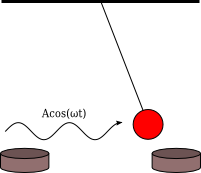
\includegraphics{pendulum.png}
\caption{Przykład realizacji układu bistabilnego.}\end{figure}

\end{description}

2 Drugi przykład realizacji: Obwód elektroniczny, który jest szczegółowo opisany w pracy:
\begin{quote}

B. K. Jones and G. Trefan, Am. J. Phys. 69 (2001) str. 464.
``The Duffing oscillator: A precise electronic analog chaos demonstrator
for the undergraduate laboratory ``
\end{quote}


\begin{verbatim}
# Przeskalowany potencjał bistabilny: a=b=1
p = plot(0.25*x^4 - 0.5*x^2, (x,-1.6,1.6), figsize=(6,4), axes_labels=[r'$x$',r'$V(x)$'], color="blue")
p += text("$-x_s$",(-1,0.025),fontsize=16, color='black')
p += text("$x_s$",(1,0.025),fontsize=16, color='black')
p.show()
\end{verbatim}



\subsection{Skalowanie}
\label{ch2/chII011:skalowanie}
Układ opisany powyżej zawiera 6 parametrów. Część parametrów można wyeliminować poprzez przeskalowanie równania do postaci bezwymiarowej. Istnieje kilka  możliwości. Zwykle zaczynamy od skalowania czasu i położenia. Nowy bezwymiarowy czas $\tau$ ma postać:
\phantomsection\label{ch2/chII011:equation-eqn3}\begin{gather}
\begin{split}s = \frac{t}{\tau_0}, \qquad \tau_0^2 = \frac{m}{a}\end{split}\label{ch2/chII011-eqn3}
\end{gather}
Nowe bezwymiarowe położenie definiujemy jako
\phantomsection\label{ch2/chII011:equation-eqn4}\begin{gather}
\begin{split}X = \frac{x}{L}, \qquad L^2 = \frac{a}{b}\end{split}\label{ch2/chII011-eqn4}
\end{gather}
Wówczas bezwymiarowa postać równania ruchu jest następująca:
\phantomsection\label{ch2/chII011:equation-eqn5}\begin{gather}
\begin{split}\ddot X = X - X^3 - \gamma_0 \dot X + A_0 \cos(\omega_0 s), \qquad X(0) = X_0, \quad  \dot X(0) = \dot X_0\end{split}\label{ch2/chII011-eqn5}
\end{gather}
Obecnie występują 3 przeskalowane parametry:
\phantomsection\label{ch2/chII011:equation-eqn6}\begin{gather}
\begin{split} \gamma_0  = \frac{\tau_0^2}{m L} \gamma, \qquad A_0 = \frac{\tau_0^2}{m L} A, \qquad \omega_0 = \tau_0 \Omega\end{split}\label{ch2/chII011-eqn6}
\end{gather}
W dalszej części będziemy posługiwali się tylko i wyłącznie przeskalowanym równaniem. Dlatego wygodnie będzie używać ``starych'' oznaczeń: Bedziemy analizowali równanie w postaci
\phantomsection\label{ch2/chII011:equation-eqn7}\begin{gather}
\begin{split}\ddot x = x - x^3 - \gamma \dot x + A \cos(\omega_0 t ), \qquad x(0) = x_0, \quad  \dot x(0) = \dot y_0 = v_0\end{split}\label{ch2/chII011-eqn7}
\end{gather}
gdzie przeskalowany potencjał
\phantomsection\label{ch2/chII011:equation-eqn7a}\begin{gather}
\begin{split}V(x) = - \int F(x) dx = \frac{1}{4} x^4 - \frac{1}{2} x^2\end{split}\label{ch2/chII011-eqn7a}
\end{gather}
Przeskalowane równanie jest w takiej postaci, że przyjmujemy wartości parametrów $m=1,  a=1,  b=1$.


\subsection{Krok 1. Układ zachowawczy}
\label{ch2/chII011:krok-1-uklad-zachowawczy}
W pierwszym  kroku rozpatrujemy najprostszy przypadek (pamiętajmy o przeskalowanej postaci, w której masa cząstki $m=1$)):
\phantomsection\label{ch2/chII011:equation-eqn8}\begin{gather}
\begin{split}\ddot x = x - x^3 = - V'(x), \qquad x(0) = x_0, \quad  \dot x(0) = v(0) =  v_0\end{split}\label{ch2/chII011-eqn8}
\end{gather}
Jest on równoważny układowi 2 równań różniczkowych, autonomicznych, pierwszego rzędu:
\phantomsection\label{ch2/chII011:equation-eqn9}\begin{gather}
\begin{split}\dot x = v, \qquad x(0) = x_0,\end{split}\label{ch2/chII011-eqn9}\\\begin{split}\dot v = x - x^3, \qquad v(0) = v_0.\end{split}\notag
\end{gather}
Oznacza to, że przestrzeń fazowa jest 2-wymiarowa.

Taki przypadek był już rozpatrywany: jest to układ zachowawczy o jednym stopniu swobody. Istnieje jedna stała ruchu (jedna całka ruchu), a mianowicie całkowita energia układu:
\phantomsection\label{ch2/chII011:equation-eqn10}\begin{gather}
\begin{split}\frac{1}{2} \dot x^2(t) + V(x(t)) = const. = E  = E_k + E_p = \frac{1}{2} \dot x^2(0) + V(x(0)) = \frac{1}{2}  v_0^2 + V(x_0)\end{split}\label{ch2/chII011-eqn10}
\end{gather}
na którą składa się energia kinetyczna $E_k$ oraz energia potencjalna $E_p$.  Stała $E$ jest określona przez warunki początkowe $x(0) = x_0$ oraz $v(0) = v_0$.  Ponieważ jest zachowana całkowita energia układu, ruch jest periodyczny. Nie istnieją atraktory i nie istnieją  asymptotycznie stabilne stany stacjonarne. Krzywe fazowe są zamknięte co oznacza że  cząstka porusza się periodycznie w czasie. W zależności od warunków początkowych, amplituda dragań jest większa lub mniejsza, ponieważ warunki początkowe wyznaczają wartość stałej ruchu $E$. Jeżeli dwa warunki początkowe $(x_{01}, v_{01})$  oraz  $(x_{02}, v_{02})$ nieznacznie się różnią, np. w sensie odległości:
\phantomsection\label{ch2/chII011:equation-eqn11}\begin{gather}
\begin{split}| [x_{01}^2 +  v_{01}^2] - [x_{02}^2 +  v_{02}^2] | << 1\end{split}\label{ch2/chII011-eqn11}
\end{gather}
to krzywe fazowe nieznacznie się różnią i ruch cząstki dla tych dwóch warunków początkowych nieznacznie się różni. Mówimy wówczas, że układ jest nieczuły na zmianę warunków początkowych.  Jak widać z powyższego wzoru, dwa różne warunki początkowe oznaczają, że układ ma dwie różne energie $E$. To z kolei oznacza, że częstości ruchu periodycznego także będą różne.  Różnica częstości powoduje, że cząstki  będą się powoli oddalać od siebie, ale tempo oddalania będzie liniowe w czasie.  Gdyby tempo oddalania było znacznie szybsze, a mianowicie rosło eksponencjalnie w czasie, zachowanie takie nazwalibyśmy chaotycznym.  Do tego problemu powrócimy poniżej, ponieważ jest on kluczowym dla zrozumienia chaotycznego zachowania się układu.

Poniżej przedstawiamy potencjał i  krzywe fazowe dla tego przypadku.


\begin{verbatim}
#parametry dla wizualizacji
var('x v')
x0 = 1.5
v0 = 0.2
E = 0.25*x0^4 - 0.5*x0^2 + v0^2
#
#prawo zachowania energii
V=0.25*x^4 - 0.5*x^2
PZE = v^2 + V == E
#
#wychylenia ekstremalne
print "ekstremalne wychylenia dla (x0,v0) = (%.2f,%.2f)"%(x0,v0)
rozw = solve(PZE(v=0), x); show(rozw)
xmin = min([i.rhs() for i in rozw if imag(i.rhs()) == 0])
xmax = max([i.rhs() for i in rozw if imag(i.rhs()) == 0])
#
#i jego rozwiązanie
print "ekstremalne prędkości dla (x0,v0) = (%.2f,%.2f)"%(x0,v0)
rozw = solve(PZE, v); show(rozw)
v1=rozw[0].rhs()
v2=rozw[1].rhs()
vmax = abs(v1(x=0))
#
#krzywe fazowe
start_point = (x0,V(x=x0))
p0 = point(start_point,size=30) + text(r"$  x_0$",start_point,vertical_alignment='bottom',horizontal_alignment='left')
p1 = plot(V,(x,xmin,xmax))
p21 = plot(v1, (x,xmin,xmax), color='red')
p22 = plot(v2, (x,xmin,xmax), color='green')
(p0+p1).show(figsize=4)
(p21+p22).show(figsize=4)
\end{verbatim}



\subsection{Krok 2. Układ dysypatywny czyli wpływ tarcia.}
\label{ch2/chII011:krok-2-uklad-dysypatywny-czyli-wplyw-tarcia}
W drugim  kroku dodajemy tarcie i rozpatrujemy równanie ruchu w postaci:
\phantomsection\label{ch2/chII011:equation-eqn12}\begin{gather}
\begin{split}\ddot x =  x - x^3 -\gamma \dot x , \qquad x(0) = x_0, \quad  \dot x(0) = v(0) =  v_0\end{split}\label{ch2/chII011-eqn12}
\end{gather}
Jest on równoważny układowi 2 równań różniczkowych, autonomicznych, pierwszego rzędu:
\phantomsection\label{ch2/chII011:equation-eqn13}\begin{gather}
\begin{split}\dot x = v, \qquad x(0) = x_0,\end{split}\label{ch2/chII011-eqn13}\\\begin{split}\dot v = x - x^3 -\gamma v , \qquad v(0) = v_0.\end{split}\notag
\end{gather}
Oznacza to, że przestrzeń fazowa jest 2-wymiarowa.

Taki przypadek był także rozpatrywany: jest to układ dysypatywny o jednym stopniu swobody. Nie istnieje już stała ruchu $E$.  Całkowita energia układu maleje w czasie.  W tym układzie  istnieją 3 stany stacjonarne. Stany te określone są przez równanie:
\phantomsection\label{ch2/chII011:equation-eqn14}\begin{gather}
\begin{split}x-x^3=0, \qquad \mbox{stąd} \qquad x_{s0}=0, \quad x_{s1} = 1, \quad x_{s2} = -1\end{split}\label{ch2/chII011-eqn14}
\end{gather}
Stany stacjonarne $x_{s1} = 1$ oraz $x_{s2} = -1$  są  stabilne. Stan $x_{s0}=0$ jest niestabilny. Istnieją 2 atraktory  $A_1= x_{s1} = 1$ oraz $A_2= x_{s2} = -1$ i  2 obszary przyciągania $B(A_1)$ oraz $B(A_2)$, których suma mnogościowa $B(A_1) \cup  B(A_2) = R^2$ jest całą płaszczyzną.  Krzywe fazowe  zawsze dążą do jednego z atraktorów lub do niestabilnego stanu stacjonarnego. Jeżeli dwa warunki początkowe $(x_{01}, v_{01})$  oraz  $(x_{02}, v_{02})$ nieznacznie się różnią np. w sensie odległości:
\phantomsection\label{ch2/chII011:equation-eqn15}\begin{gather}
\begin{split}| [x_{01}^2 +  v_{01}^2] - [x_{02}^2 +  v_{02}^2] | << 1\end{split}\label{ch2/chII011-eqn15}
\end{gather}
i są w tym samym obszarze przyciągania, to krzywe fazowe nieznacznie się różnią i ruch cząstki dla tych dwóch warunków początkowych nieznacznie się różni. Mówimy wówczas, że układ jest nieczuły na zmianę warunków początkowych. Natomiast jeżeli dwa warunki początkowe $(x_{01}, v_{01}) \in B(A_1)$  oraz  $(x_{02}, v_{02}) \in B(A_2)$ nieznacznie się różnią, ale są w dwóch obszarach przyciągania $B(A_1)$ oraz $B(A_2)$, to trajektorie zaczną po pewnym czasie różnić się znacznie, będą przyciągane do dwóch różnych atraktorów  i będą dążyć  do dwóch różnych stanów stacjonarnych :math:{}` x\_\{s1\} = 1{}` oraz :math:{}` x\_\{s2\} = -1{}`. Tym niemniej, w takiej sytuacji mówimy, że układ jest nieczuły na zmianę warunków początkowych w sensie o którym mowa powyżej.
\begin{figure}[htbp]
\centering
\capstart

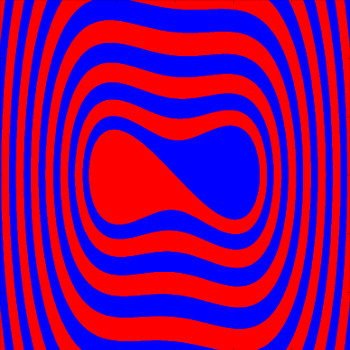
\includegraphics{baseny_tarcie.jpg}
\caption{Diagram basenów przyciągania dla potencjału bistabilnego}\end{figure}

Kolor niebieski to obszar warunków początkowych które są ``przyciągane''  do atraktora $(1, 0)$, do prawego
minimum potencjału. Kolor czerwony to obszar warunków początkowych które są ``przyciągane''  do atraktora
$(-1, 0)$, do lewego minimum potencjału. W zależności od wartości stałej tłumienia $\gamma$, diagram
ten przybiera nieco inne kształty, ale struktura dwu-kolorowych pasów pozostaje. Brzeg obszarów przyciągania jest
gładką krzywą, której wymiar wynosi 1. Jeżeli warunki początkowe są położone dokładnie na tym brzegu, to cząstka
porusza się do niestabilnego stanu stacjonarnego $(x=0, v=0)$ (maksimum potencjału).


\begin{verbatim}
# wykresy dla przypadku z tłumieniem
var('x v')
x01, v01 = 1.50, 0
x02, v02 = 1.52, 0
#
# siła
F = x-x^3
V = -integrate(F,x)
#
# tarcie: parametr gamma
g = 0.1
#
# numeryczne rozwiazanie równań ruchu
T = srange(0,20*pi,0.01)
num1 = desolve_odeint(vector([v,F-g*v]), [x01,v01], T, [x,v])
num2 = desolve_odeint(vector([v,F-g*v]), [x02,v02], T, [x,v])
#
#krzywe fazowe
lt  = plot(V, (x, -max([abs(x01),abs(x02)]),max([abs(x01),abs(x02)])), color='black', figsize=4)
lt += point((x01,V(x=x01)), color='green', size=50, axes_labels=['$x$','$V(x)$'])
lt += point((x02,V(x=x02)), color='red', size=50)
lb  = list_plot(num1.tolist(), plotjoined=1, color='green', axes_labels=['$x(t)$','$v(t)$'])
lb += list_plot(num2.tolist(), plotjoined=1, color='red', figsize=4)
rt  = list_plot(zip(T,num1[:,0].tolist()), plotjoined=1, color='green', axes_labels=['$t$','$x(t)$'])
rt += list_plot(zip(T,num2[:,0].tolist()), plotjoined=1, color='red', figsize=4)
rb  = list_plot(zip(T,num1[:,1].tolist()), plotjoined=1, color='green', axes_labels=['$t$','$v(t)$'])
rb += list_plot(zip(T,num2[:,1].tolist()), plotjoined=1, color='red', figsize=4)
#
html("""
<p align='center'>rozwiązania z warunkami początkowymi
<span style="color:green">($x_{01},v_{01}$)=(%.2f,%.2f)</span>
<span style="color:red">($x_{02},v_{02}$)=(%.2f,%.2f)</span>
dążą do tego samego atraktora:
(x,v)=(-1,0)
</p>
"""%(x01,v01,x02,v02))
html.table([[lt,rt],[lb,rb]])
\end{verbatim}


Na powyższym zestawie rysunków,  2 warunki początkowe leżą w tym samym obszarze  przyciągania  atraktora $(-1, 0)$. Oznacza to, że 2 warunki początkowe są umiejscowione w czerwonym obszarze na diagramie basenów przyciągania pokazanym powyżej. Układ nie jest czuły na zmianę warunków początkowych, gdy leżą one w tym samym basenie przyciągania.


\begin{verbatim}
# wykresy dla przypadku z tłumieniem
var('x v')
x01, v01 = 1.58, 0
x02, v02 = 1.57, 0
#
# siła
F = x-x^3
V = -integrate(F,x)
#
# tarcie: parametr gamma
g = 0.1
#
# numeryczne rozwiazanie równań ruchu
T = srange(0,20*pi,0.01)
num1 = desolve_odeint(vector([v,F-g*v]), [x01,v01], T, [x,v])
num2 = desolve_odeint(vector([v,F-g*v]), [x02,v02], T, [x,v])
#
# wykresy funkcji
lt  = plot(V, (x, -max([abs(x01),abs(x02)]),max([abs(x01),abs(x02)])),color='black',  figsize=4)
lt += point((x01,V(x=x01)), color='blue', size=50, axes_labels=['$x$','$V(x)$'])
lt += point((x02,V(x=x02)), color='red', size=50)
lb  = list_plot(num1.tolist(), plotjoined=1, color='blue', axes_labels=['$x(t)$','$v(t)$'])
lb += list_plot(num2.tolist(), plotjoined=1, color='red', figsize=4)
rt  = list_plot(zip(T,num1[:,0].tolist()), plotjoined=1, color='blue', axes_labels=['$t$','$x(t)$'])
rt += list_plot(zip(T,num2[:,0].tolist()), plotjoined=1, color='red', figsize=4)
rb  = list_plot(zip(T,num1[:,1].tolist()), plotjoined=1, color='blue', axes_labels=['$t$','$v(t)$'])
rb += list_plot(zip(T,num2[:,1].tolist()), plotjoined=1, color='red', figsize=4)
#
html("""
<p align='center'>rozwiązania z warunkami początkowymi
<span style="color:blue">($x_{01},v_{01}$)=(%.2f,%.2f)</span>
<span style="color:red">($x_{02},v_{02}$)=(%.2f,%.2f)</span>
dążą do różnych atraktorów:
<span style="color:blue">(x,v)=(1,0)</span>
<span style="color:red">(x,v)=(-1,0)</span>
</p>
"""%(x01,v01,x02,v02))
html.table([[lt,rt],[lb,rb]])
\end{verbatim}


Na powyższym zestawie rysunków,  2 warunki początkowe leżą w dwóch różnych obszarach  przyciągania.  Oznacza to, że 1 warunek  początkowy leży w  niebieskim obszarze na diagramie basenów przyciągania, natomiast  2 warunek  początkowy leży w  czerwonym obszarze na diagramie basenów przyciągania. Te dwa warunki początkowe leżą blisko brzegu 2 basenów przyciągania. Dlatego układ jest czuły na zmianę warunków początkowych, pod warunkiem że leżą one w dwóch różnych basenach przyciągania. Ale to nie jest jeszcze kryterium własności chaotyczych układu.


\subsection{Krok 3. Układ z tarciem i periodyczną siłą.}
\label{ch2/chII011:krok-3-uklad-z-tarciem-i-periodyczna-sila}
W trzecim kroku dodajemy siłę periodyczną w czasie  i rozpatrujemy równanie ruchu w wyjściowej pełnej postaci:
\phantomsection\label{ch2/chII011:equation-eqn16}\begin{gather}
\begin{split}\ddot x =  x - x^3 -\gamma \dot x  +  A \cos (\omega_0 t) , \qquad x(0) = x_0, \quad  \dot x(0) = v(0) =  v_0\end{split}\label{ch2/chII011-eqn16}
\end{gather}
Jest on równoważny układowi 3 równań różniczkowych, autonomicznych, pierwszego rzędu:
\phantomsection\label{ch2/chII011:equation-eqn17}\begin{gather}
\begin{split}\dot x = v, \qquad x(0) = x_0,\end{split}\label{ch2/chII011-eqn17}\\\begin{split}\dot v = x - x^3 -\gamma v + A \cos z , \qquad v(0) = v_0,\end{split}\notag\\\begin{split}z = \omega_0, \qquad z(0) = 0.\end{split}\notag
\end{gather}
Oznacza to, że przestrzeń fazowa jest 3-wymiarowa.

Matematycy wolą przepisać powyższy układ równań dla ``tradycyjnych''  3 zmiennych $(x, y, z)$ w postaci:
\phantomsection\label{ch2/chII011:equation-eqn18}\begin{gather}
\begin{split}\dot x = y, \qquad x(0) = x_0,\end{split}\label{ch2/chII011-eqn18}\\\begin{split}\dot y = x - x^3 -\gamma y + A \cos z , \qquad y(0) = y_0,\end{split}\notag\\\begin{split}z = \omega_0, \qquad z(0) = 0.\end{split}\notag
\end{gather}
czyli prędkość cząstki $v$ jest teraz oznaczona jako $v=y$.

Okazuje się, że pełny układ wykazuje radykalnie inne własności od poprzednich 2 przypadków. Z punktu widzenia fizyki mamy taki oto proces:  Cząstka porusza się w bistabilnym potencjale. Ponieważ potencjał dąży do nieskończoności gdy położenie dąży do nieskończoności, ruch cząstki jest ograniczony; cząstka jest uwięziona w potencjale i nie może uciec do nieskończoności. Siła tarcia pcha cząstkę do jednego ze (``starych'') stanów stacjonarnych  $x_{s1}$  lub $x_{s2}$. Z kolei zewnętrzna siła periodyczna w czasie pompuje energię do układu i przeciwdziała sile tarcia. Cząstka już nie dąży do stanu stacjonarnego, nie zatrzyma się dla długich czasów ale będzie  ciągle poruszać się i nigdy już nie spocznie. Istotne stają się efekty inercjalne związane z masą czastki, które są odzwierciedlone w wyrazie $\dot y$, czyli przyśpieszeniu cząstki. Istotne jest to, że nie jest to ruch przetłumiony. W konsekwencji układ nie posiada stanu stacjonarnego w postaci punktu w przestrzeni fazowej jak to było w przypadku 2. Wszystkie te powyższe czynniki stają się istotne dla zrozumienia  skomplikowanych i złożonych własności ewolucji cząstki.


\begin{verbatim}
# przykładowa trajektoria  (górny wykres)
# wraz z krzywą fazową (dolny wykres)
var('x y z')
T = srange(0,150*pi,0.01)
sol=desolve_odeint( vector([y,x-x^3-0.26*y+0.3*cos(z), 1]), [0.1,0.1,0],T,[x,y,z])
t = line(zip(T,sol[:,0]), figsize=(12,4), axes_labels=["$t$","$x(t)$"], frame=1, axes=0)
b = line(zip(sol[:,0],sol[:,1]), figsize=(12,4), axes_labels=["$x(t)$","$v(t)$"], frame=1, axes=0)
html.table([[t],[b]])
\end{verbatim}



\subsection{Ruch periodyczny o okresie 1}
\label{ch2/chII011:ruch-periodyczny-o-okresie-1}
W modelu występują 3 bezwymiarowe parametry: współczynnik tarcia $\gamma$, amplituda zewnętrznej siły $A$ oraz częstość drgań $\omega_0$ siły periodycznej w czasie. Poniżej pokażemy kilka charakterystycznych trajektorii układu. Zaczniemy od prostej periodycznej ewolucji, ruchu okresowego o tzw. okresie 1.

Załóżmy następujące wartości parametrów:
\phantomsection\label{ch2/chII011:equation-eqn19}\begin{gather}
\begin{split}\gamma = 0.15, \qquad A = 0.3, \qquad \omega_0 = 1\end{split}\label{ch2/chII011-eqn19}
\end{gather}
W tym przypadku obserwujemy regularny ruch. Jeżeli nieco zaburzymy warunki początkowe, to nowy ruch jest także regularny (trzeba być ostrożnym, gdy mówimy ``nieco zaburzymy'').


\begin{verbatim}
# wykresy dla przypadku z tłumieniem
var('x y z')
x0, y0, z0 = 0.1,0.1,0
kolor = 'green'
#
# siła
F = x-x^3
V = -integrate(F,x)
#
# tarcie: parametr gamma
g = 0.1
A = 0.3
w = 1
#
# układ różniczkowych równań ruchu
dx = y
dy = F - g*y + A*cos(z)
dz = w
#
# numeryczne rozwiazanie równań ruchu
T = srange(0,30*pi,0.01)
num = desolve_odeint(vector([dx,dy,dz]), [x0,y0,z0], T, [x,y,z])
#
# wykresy funkcji
xmin = 1.5
lt  = plot(V, (x,-xmin,xmin), figsize=4)
lt += point((x0,V(x=x0)), color=kolor, size=50, axes_labels=['$x$','$V(x)$'])
lb  = list_plot(zip(num[:,0],num[:,1]), plotjoined=1, color=kolor, axes_labels=['$x(t)$','$v(t)$'], figsize=4)
rt  = list_plot(zip(T,num[:,0].tolist()), plotjoined=1, color=kolor, axes_labels=['$t$','$x(t)$'], figsize=4)
rb  = list_plot(zip(T,num[:,1].tolist()), plotjoined=1, color=kolor, axes_labels=['$t$','$v(t)$'], figsize=4)
#
html("""Układ równań różniczkowych
$\dot{x} = %s$
$\dot{y} = %s$
$\dot{z} = %s$
z warunkami początkowymi
$(x_0,y_0,z_0) = (%.2f,%.2f,%.2f)$
"""%(dx,dy,dz,x0,y0,z0))
html.table([[lt,rt],[lb,rb]])
\end{verbatim}


Przyjrzyjmy sie teraz dwóm trajektoriom startującym z bliskich warunków początkowych. Rozpatrzmy ich początkową i asymptotyczną (dla długich czasów) ewolucję.


\begin{verbatim}
# wykresy dla przypadku z tłumieniem
var('x y z')
x01, y01, z01 = 0.1,0.1,0
x02, y02, z02 = 0.11,0.1,0
#
# siła
F = x-x^3
V = -integrate(F,x)
#
# tarcie: parametr gamma
g = 0.1
A = 0.3
w = 1
#
# układ różniczkowych równań ruchu
dx = y
dy = F - g*y + A*cos(z)
dz = w
#
# numeryczne rozwiazanie równań ruchu
T = srange(0,200*pi,0.01)
num1 = desolve_odeint(vector([dx,dy,dz]), [x01,y01,z01], T, [x,y,z])
num2 = desolve_odeint(vector([dx,dy,dz]), [x02,y02,z02], T, [x,y,z])
#
lnum = int(len(num1[:,0])/10)
trans1 = num1[:lnum]
asymp1 = num1[-lnum:]
trans2 = num2[:lnum]
asymp2 = num2[-lnum:]
#
# wykresy funkcji
lt = list_plot(zip(trans1[:,0],trans1[:,1]), plotjoined=1, color='green', axes_labels=['$x(t)$','$v(t)$'], figsize=4)
lt += list_plot(zip(trans2[:,0],trans2[:,1]), plotjoined=1, color='red')
rt = list_plot(zip(T[:lnum],trans1[:,0].tolist()), plotjoined=1, color='green', axes_labels=['$t$','$x(t)$'], figsize=4)
rt += list_plot(zip(T[:lnum],trans2[:,0].tolist()), plotjoined=1, color='red')
lb = list_plot(zip(asymp1[:,0],asymp1[:,1]), plotjoined=1, color='green', axes_labels=['$x(t)$','$v(t)$'], figsize=4)
lb += list_plot(zip(asymp2[:,0],asymp2[:,1]), plotjoined=0, color='red')
rb = list_plot(zip(T[-lnum:],asymp1[:,0].tolist()), plotjoined=1, color='green', axes_labels=['$t$','$x(t)$'], figsize=4)
rb += list_plot(zip(T[-lnum:],asymp2[:,0].tolist()), plotjoined=1, color='red')
#
html("""Układ równań różniczkowych
$\dot{x} = %s$
$\dot{y} = %s$
$\dot{z} = %s$
z różnymi warunkami początkowymi
<span style="color:green;">$(x_{01},y_{01},z_{01}) = (%.2f,%.2f,%.2f)$</span>
<span style="color:red;">$(x_{02},y_{02},z_{02}) = (%.2f,%.2f,%.2f)$</span>
"""%(dx,dy,dz,x01,y01,z01,x02,y02,z02))
html.table([[lt,rt],[lb,rb]])
\end{verbatim}


Na dwóch górnych diagramach przedstawioną reżim krótkich czasów. Ponieważ 2 warunki początkowe nieco się różnią, więc początkowa ewolucja nieco się różni. Kolor czerwony i zielony jest rozróżnialny na prawym górnym rysunku pokazującym ewolucję $x(t)$ dla krótkich czasów.  Jeżeli przyjrzymy się reżimowy długich czasów (dwa dolne diagramy) to zauważymy duże podobieństwo w ewolucji: krzywe fazowe są zamknięte więc jest to prosty ruch periodyczny, przypominający nieco zdeformowaną funkcję typu $\sin(\alpha t)$ czy też $\cos(\alpha t)$. Jest to funkcja okresowa z charakterystycznym jednym jedynym  okresem $T$. Dlatego mówimy, że jest ruch periodyczny o okresie 1. Dwie krzywe $x(t)$ na dolnym prawym rysunku nie są rozróżnialne.

Można zrobić doświadczenie numeryczne i wybierać różne warunki początkowe. Zobaczymy, że trajektorie dążą do tego samego okresowego rozwiązania, są przyciagane do tego okresowego rozwiązania. Innymi słowy, ta krzywa fazowa o okresie 1  jest ATRAKTOREM.  Atraktor ten nazywa się periodycznym atraktorem o okresie 1 lub 1-okresowym  atraktorem. Można by postawić pytanie: jak wygląda basen przyciągania dla tego atraktora. Aby dać odpowiedź na to pytanie należy zbadać numerycznie np. kwadrat warunków początkowych  $(x_0, y_0)$ i wybrać te warunki początkowe które dążą do powyższej krzywej fazowej o okresie 1. Okazuje się, że basen przyciągania jest ``porządnym'' zbiorem, którego brzeg jest gładką krzywą, podobnie jak w przypadku zilustrowanym powyżej dla układu tylko z tarciem, bez siły okresowej.


\subsection{Ruch periodyczny o okresie 3}
\label{ch2/chII011:ruch-periodyczny-o-okresie-3}
Załóżmy następujące wartości parametrów:
\phantomsection\label{ch2/chII011:equation-eqn20}\begin{gather}
\begin{split}\gamma = 0.22, \qquad A = 0.3, \qquad \omega_0 = 1\end{split}\label{ch2/chII011-eqn20}
\end{gather}
W tym przypadku obserwujemy także periodyczny ruch, ale nieco bardziej skomplikowany. Nie jest to prosty periodyczny ruch, ale tzw. ruch o okresie 3, tzn. teraz okres jest 3 razy dłuższy niż w poprzednim przypadku.


\begin{verbatim}
# wykresy dla przypadku z tłumieniem
var('x y z')
x0, y0, z0 = 0.1,0.1,0
kolor = 'red'
#
# siła
F = x-x^3
V = -integrate(F,x)
#
# tarcie: parametr gamma
g = 0.22
A = 0.3
w = 1
#
# układ różniczkowych równań ruchu
dx = y
dy = F - g*y + A*cos(z)
dz = w
#
# numeryczne rozwiazanie równań ruchu
T = srange(0,20*pi,0.01)
num = desolve_odeint(vector([dx,dy,dz]), [x0,y0,z0], T, [x,y,z])
#
# wykresy funkcji
xmin = 1.5
lt  = plot(V, (x,-xmin,xmin), figsize=4)
lt += point((x0,V(x=x0)), color=kolor, size=50, axes_labels=['$x$','$V(x)$'])
lb  = list_plot(zip(num[:,0],num[:,1]), plotjoined=1, color=kolor, axes_labels=['$x(t)$','$v(t)$'], figsize=4)
rt  = list_plot(zip(T,num[:,0].tolist()), plotjoined=1, color=kolor, axes_labels=['$t$','$x(t)$'], figsize=4)
rb  = list_plot(zip(T,num[:,1].tolist()), plotjoined=1, color=kolor, axes_labels=['$t$','$v(t)$'], figsize=4)
#
html("""Układ równań różniczkowych
$\dot{x} = %s$
$\dot{y} = %s$
$\dot{z} = %s$
z warunkami początkowymi
$(x_0,y_0,z_0) = (%.2f,%.2f,%.2f)$
"""%(dx,dy,dz,x0,y0,z0))
html.table([[lt,rt],[lb,rb]])
\end{verbatim}


I znów zobaczymy, jak początkowa ewolucja różni się od tej po długim czasie.


\begin{verbatim}
# wykresy dla przypadku z tłumieniem
var('x y z')
x01, y01, z01 = 0.10,0.1,0
x02, y02, z02 = 0.11,0.1,0
#
# siła
F = x-x^3
V = -integrate(F,x)
#
# tarcie: parametr gamma
g = 0.22
A = 0.3
w = 1
#
# układ różniczkowych równań ruchu
dx = y
dy = F - g*y + A*cos(z)
dz = w
#
# numeryczne rozwiazanie równań ruchu
T = srange(0,200*pi,0.01)
num1 = desolve_odeint(vector([dx,dy,dz]), [x01,y01,z01], T, [x,y,z])
num2 = desolve_odeint(vector([dx,dy,dz]), [x02,y02,z02], T, [x,y,z])
#
lnum = int(len(num1[:,0])/10)
trans1 = num1[:lnum]
asymp1 = num1[-lnum:]
trans2 = num2[:lnum]
asymp2 = num2[-lnum:]
#
# wykresy funkcji
lt = list_plot(zip(trans1[:,0],trans1[:,1]), plotjoined=1, color='green', axes_labels=['$x(t)$','$v(t)$'], figsize=4)
lt += list_plot(zip(trans2[:,0],trans2[:,1]), plotjoined=1, color='red')
rt = list_plot(zip(T[:lnum],trans1[:,0].tolist()), plotjoined=1, color='green', axes_labels=['$t$','$x(t)$'], figsize=4)
rt += list_plot(zip(T[:lnum],trans2[:,0].tolist()), plotjoined=1, color='red')
lb = list_plot(zip(asymp1[:,0],asymp1[:,1]), plotjoined=1, color='green', axes_labels=['$x(t)$','$v(t)$'], figsize=4)
lb += list_plot(zip(asymp2[:,0],asymp2[:,1]), plotjoined=0, color='red')
rb = list_plot(zip(T[-lnum:],asymp1[:,0].tolist()), plotjoined=1, color='green', axes_labels=['$t$','$x(t)$'], figsize=4)
rb += list_plot(zip(T[-lnum:],asymp2[:,0].tolist()), plotjoined=1, color='red')
#
html("""Układ równań różniczkowych
$\dot{x} = %s$
$\dot{y} = %s$
$\dot{z} = %s$
z różnymi warunkami początkowymi
<span style="color:green;">$(x_{01},y_{01},z_{01}) = (%.2f,%.2f,%.2f)$</span>
<span style="color:red;">$(x_{02},y_{02},z_{02}) = (%.2f,%.2f,%.2f)$</span>
"""%(dx,dy,dz,x01,y01,z01,x02,y02,z02))
html.table([[lt,rt],[lb,rb]])
\end{verbatim}


Dla długich czasów, krzywe fazowe są zamknięte, ale nie są  to krzywe typu zdeformowana elipsa.  To są krzywe z 2 pętelkami. Tym niemniej, ruch jest periodyczny.

Podobnie jak poprzednim przypadku, można zrobić doświadczenie numeryczne i wybierać różne warunki początkowe. Zobaczymy, że wiele trajektorii dąży do tej samej  okresowej orbity, są one  przyciagane do tej  zamkniętek krzywej fazowej. Innymi słowy, ta krzywa fazowa o okresie 3  jest ATRAKTOREM.  Atraktor ten nazywa się periodycznym atraktorem o okresie 3 lub 3-okresowym  atraktorem.  Basen przyciągania dla tego atraktora  na płaszczyźnie warunków początkowych $(x_0, y_0)$  jest ``porządnym'' zbiorem o wymiarze 2 (czyli kawałek płaszczyzny), którego brzeg jest gładką krzywą.


\subsection{Ruch chaotyczny}
\label{ch2/chII011:ruch-chaotyczny}
Załóżmy następujące wartości parametrów:
\phantomsection\label{ch2/chII011:equation-eqn21}\begin{gather}
\begin{split}\gamma = 0.25, \qquad A = 0.3, \qquad \omega_0 = 1\end{split}\label{ch2/chII011-eqn21}
\end{gather}
W tym przypadku obserwujemy ruch, który wydaje się być wyjątkowo nieregularny, chaotyczny.


\begin{verbatim}
# wykresy dla przypadku chaotycznego
var('x y z')
x0, y0, z0 = 0.1,0.1,0
kolor = 'firebrick'
#
# siła
F = x-x^3
V = -integrate(F,x)
#
# tarcie: parametr gamma
g = 0.25
A = 0.3
w = 1
#
# układ różniczkowych równań ruchu
dx = y
dy = F - g*y + A*cos(z)
dz = w
#
# numeryczne rozwiazanie równań ruchu
T = srange(0,50*pi,0.01)
num = desolve_odeint(vector([dx,dy,dz]), [x0,y0,z0], T, [x,y,z])
#
# wykresy funkcji
xmin = 1.5
lt  = plot(V, (x,-xmin,xmin), figsize=4)
lt += point((x0,V(x=x0)), color=kolor, size=50, axes_labels=['$x$','$V(x)$'])
lb  = list_plot(zip(num[:,0],num[:,1]), plotjoined=1, color=kolor, axes_labels=['$x(t)$','$v(t)$'], figsize=4)
rt  = list_plot(zip(T,num[:,0].tolist()), plotjoined=1, color=kolor, axes_labels=['$t$','$x(t)$'], figsize=4)
rb  = list_plot(zip(T,num[:,1].tolist()), plotjoined=1, color=kolor, axes_labels=['$t$','$v(t)$'], figsize=4)
#
html("""Układ równań różniczkowych
$\dot{x} = %s$
$\dot{y} = %s$
$\dot{z} = %s$
z warunkami początkowymi
$(x_0,y_0,z_0) = (%.2f,%.2f,%.2f)$
"""%(dx,dy,dz,x0,y0,z0))
html.table([[lt,rt],[lb,rb]])
\end{verbatim}


Zobaczmy, jak tym razem ewoluują rozwiązania o 2 bliskich warunkach początkowych.


\begin{verbatim}
var('x y z')
x01, y01, z01 = 0.1,0.1,0
x02, y02, z02 = 0.11,0.1,0
#
# siła
F = x-x^3
V = -integrate(F,x)
#
# tarcie: parametr gamma
g = 0.25
A = 0.3
w = 1
#
# układ różniczkowych równań ruchu
dx = y
dy = F - g*y + A*cos(z)
dz = w
#
# numeryczne rozwiazanie równań ruchu
T = srange(0,200*pi,0.01)
num1 = desolve_odeint(vector([dx,dy,dz]), [x01,y01,z01], T, [x,y,z])
num2 = desolve_odeint(vector([dx,dy,dz]), [x02,y02,z02], T, [x,y,z])
#
lnum = int(len(num1[:,0])/10)
trans1 = num1[:lnum]
asymp1 = num1[-lnum:]
trans2 = num2[:lnum]
asymp2 = num2[-lnum:]
#
# wykresy funkcji
lt = list_plot(zip(trans1[:,0],trans1[:,1]), plotjoined=1, color='green', axes_labels=['$x(t)$','$v(t)$'], figsize=4)
lt += list_plot(zip(trans2[:,0],trans2[:,1]), plotjoined=1, color='red')
rt = list_plot(zip(T[:lnum],trans1[:,0].tolist()), plotjoined=1, color='green', axes_labels=['$t$','$x(t)$'], figsize=4)
rt += list_plot(zip(T[:lnum],trans2[:,0].tolist()), plotjoined=1, color='red')
lb = list_plot(zip(asymp1[:,0],asymp1[:,1]), plotjoined=1, color='green', axes_labels=['$x(t)$','$v(t)$'], figsize=4)
lb += list_plot(zip(asymp2[:,0],asymp2[:,1]), plotjoined=1, color='red')
rb = list_plot(zip(T[-lnum:],asymp1[:,0].tolist()), plotjoined=1, color='green', axes_labels=['$t$','$x(t)$'], figsize=4)
rb += list_plot(zip(T[-lnum:],asymp2[:,0].tolist()), plotjoined=1, color='red')
#
html("""Układ równań różniczkowych
$\dot{x} = %s$
$\dot{y} = %s$
$\dot{z} = %s$
z różnymi warunkami początkowymi
<span style="color:green;">$(x_{01},y_{01},z_{01}) = (%.2f,%.2f,%.2f)$</span>
<span style="color:red;">$(x_{02},y_{02},z_{02}) = (%.2f,%.2f,%.2f)$</span>
"""%(dx,dy,dz,x01,y01,z01,x02,y02,z02))
html.table([[lt,rt],[lb,rb]])
\end{verbatim}


Początkowa ewolucja dwóch rozwiązań jest nierozróżnialna (ponieważ 2 warunki początkowe są bardzo blisko siebie). Po pewnym charakterystycznym czasie, zwanym czasem Lapunowa, trajektorie zaczynają różnić się coraz bardziej, zaczynają rozbiegać się: patrz trajektoria czerwona i zielona na dolnym prawym rysunku.
\begin{figure}[htbp]
\centering
\capstart

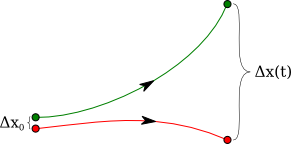
\includegraphics{chaos_traj.png}
\caption{Schematyczne trajektorie w reżimie chaotycznym.}\end{figure}

W reżimie chaotycznym, te dwie trajektorie oddalają się od siebie w eksponencjalnie szybkim tempie określonym przez zależność:
\phantomsection\label{ch2/chII011:equation-eqn22}\begin{gather}
\begin{split}|x_1(t) - x_2(t)| = |x_1(0) - x_2(0)|\mbox{e}^{\lambda t}, \qquad \lambda > 0\end{split}\label{ch2/chII011-eqn22}
\end{gather}
lub
\phantomsection\label{ch2/chII011:equation-eqn23}\begin{gather}
\begin{split}|\Delta x(t)| = |\Delta x_0|\mbox{e}^{\lambda t}, \qquad \lambda > 0\end{split}\label{ch2/chII011-eqn23}
\end{gather}
gdzie $\lambda$ nazywa sie wykładnikiem Lapunowa.

Różnice w ewolucji stają się zbyt duże i pojawia się dylemat: która trajektoria jest właściwa, skoro nasza aparatura nie rozróżnia bliskich warunków początkowych. Determinizm staje się złudnym. Nie możemy przewidywać właściwej ewolucji układu.

Przedstawiony powyżej reżim chaotyczny nie jest jedyny. W układzie istnieje wiele takich wartości parametrów $(\gamma, A, \omega)$, dla których pojawia się ruch chaotyczny. Należy nadmienić, że dla długich czasów  wiele trajektorii generowanych przez różne warunki początkowe zachowuje się bardzo podobnie, wiele trajektorii jest przyciąganych. Tu także istnieje atraktor i jego basen przyciągania. Jednakże ten atraktor jest dziwny: jego wymiar nie jest liczbą całkowitą i atraktor  jest fraktalem. Dlatego nazywa się dziwnym atraktorem.  Brzeg basenu przyciągania tego atraktora też ma dziwną strukturę  i jego wymiar jest fraktalny.
\setbox0\vbox{
\begin{minipage}{0.95\linewidth}
\textbf{Zadania}

\medskip

\begin{enumerate}
\item {} 
Niech $\gamma = 0.1, \quad \omega_0 =1.4 , \quad (x_0, y_0, z_0) = (-0.5, -0.2, 0)$.
Zmieniaj parametr $A=0.1,  0.32,  0.338,  0.35$.

Obserwuj scenariusz  podwojenia okresu:
\begin{enumerate}
\item {} 
pojawia się atraktor periodyczny o okresie 1.

\item {} 
pojawia się atraktor periodyczny o okresie 2.

\item {} 
pojawia się atraktor periodyczny o okresie 4.

\item {} 
pojawia się atraktor periodyczny o okresie 8 (trudno  trafić).

\item {} 
pojawia się ruch nieregularny, chaotyczny.

\end{enumerate}

\item {} 
Zbadaj zachowanie się układu dla następujących wartości parametrów:
$\gamma = 1.35  -  1.38, \quad A=1, \quad \omega_0 =1, \quad (x_0, y_0, z_0) = (0.0, 0.5, 0)$.

\item {} 
To samo dla wartości
$\gamma = 0.5, \quad A=0.34875, \quad \omega_0 =1, \quad (x_0, y_0, z_0) = (0,  0, 0)$

\end{enumerate}
\end{minipage}}
\begin{center}\setlength{\fboxsep}{5pt}\shadowbox{\box0}\end{center}


\section{Scenariusz przejścia do chaosu}
\label{ch2/chII012::doc}\label{ch2/chII012:scenariusz-przejscia-do-chaosu}
Zmieniając parametry układu oraz warunki początkowe, możemy sterować własnościami ewolucji czasowej. Widzieliśmy, że istnieją rozwiązania periodyczne. Może to być prosty ruch periodyczny charakteryzujący się jednym charakterystycznym okresem T (lub częstością).  Mogą to być ruchy periodyczne bardziej skomplikowane:  o okresie 2, 3, 4, itd. Zauważmy, że ruch periodyczny o okresie 3 powtarza się po czasie 3 razy dłuższym niż ruch o okresie 1. Dlatego też regularność ruchu można zaobserwować po czasie  3 razy dłuższym.   Ruch periodyczny o okresie 20 powtarza się po czasie 20 razy dłuższym niż ruch o okresie 1. Dlatego też regularność ruchu jest obserwowana po czasie 20 razy dłuższym.  Ruch periodyczny o okresie 2000 powtarza się po czasie 2000 razy dłuższym niż ruch o okresie 1. Dlatego też regularność ruchu może być rozpoznana po czasie  200 razy dłuższym.  Zwiększając periodyczność ruchu aż do nieskończoności, zauważamy że regularność ruchu powtarza się po nieskończonym czasie, czyli ruch staje się nieregularny dla obserwatora. Trajektoria wygląda tak, jakby to był ruch przypadkowy, losowy, chaotyczny. Ruch jest ciągle deterministyczny, ale skomplikowany,  niepowtarzalny, nieregularny. W niektórych przypadkach układ jest wyjątkowo wrażliwy na warunki początkowe: dla dwóch różnych, ale bardzo mało różniących się warunków początkowych, odpowiadające im trajektorie z czasem zaczynają sie różnić i odbiegać od siebie. Jeżeli zmniejszymy odległość między warunkami początkowymi, to czas po jakim można rozróżnić  2 trajektorii wydłuża się, ale prędzej czy później, trajektorie zaczynają się rozbiegać. Z praktycznego punktu widzenia, warunki początkowe można zadawać ze skończoną dokładnością, ale nie z zerową dokładnością, tak jak to się zakłada w twierdzeniach matematycznych. Dlatego też w reżimie, w którym układ jest czuły na warunki początkowe, w praktyce niepewność warunków początkowych powoduje niepewność  ewolucji czasowej. Można to sprecyzować w matematycznym sensie w następujący sposób:

Niech $x(t)$  będzie trajektorią z warunkiem początkowym $x(0)$, a $X(t)$  będzie trajektorią z warunkiem początkowym :math:{}` X(0){}`.   Niech dwa warunki początkowe różnią się o małą wielkość:
\phantomsection\label{ch2/chII012:equation-eqn1}\begin{gather}
\begin{split}|X(0) - x(0)| = \epsilon_0\end{split}\label{ch2/chII012-eqn1}
\end{gather}
gdzie $| ... |$ oznacza odległość przy zadanej metryce.  Jeżeli różnią się o taką wielkość lub mniejszą, wówczas są one  dla nas nierozróżnialne. Traktujemy je jako takie same w ramach błędu pomiarowego. Pytamy, jaka jest różnica
\phantomsection\label{ch2/chII012:equation-eqn2}\begin{gather}
\begin{split}|X(t) - x(t)| = \epsilon(t)\end{split}\label{ch2/chII012-eqn2}
\end{gather}
po czasie $t$ spowodowana niepewnością warunków początkowych $\epsilon_0$. Wrażliwość na warunki początkowe oznacza, że 2 trajektorie oddalają się od siebie w bardzo szybkim, eksponencjalnym tempie:
\phantomsection\label{ch2/chII012:equation-eqn3}\begin{gather}
\begin{split}\epsilon(t) = \epsilon_0  \mbox{e}^{\lambda t}\end{split}\label{ch2/chII012-eqn3}
\end{gather}
gdzie $\lambda$ nazywa się wykładnikiem Lapunowa. Jeżeli $\lambda < 0$ to dwie bliskie sobie trajektorie nie oddalają się od siebie. Z kolei jeżeli $\lambda > 0$ to trajektorie rozbiegają się.

Niech $\delta$ będzie dokładnością naszej aparatury do rozróżniania trajektorii.  Jeżeli $\epsilon(t) > \delta$, czyli gdy dwie  trajektorie stają się dla nas rozróżnialne, to nie możemy przewidzieć dalszej ewolucji układu:  która trajektoria jest właściwa, $x(t)$ czy $X(t)$? Po jakim czasie nasze przewidywania tracą sens?  Po takim czasie, że
\phantomsection\label{ch2/chII012:equation-eqn4}\begin{gather}
\begin{split}\epsilon(t) = \epsilon_0  \mbox{e}^{\lambda t} > \delta\end{split}\label{ch2/chII012-eqn4}
\end{gather}
czyli po czasie
\phantomsection\label{ch2/chII012:equation-eqn5}\begin{gather}
\begin{split} t > \frac{1}{\lambda}  \mbox{ln} \left[\frac{\delta}{\epsilon_0}\right]\end{split}\label{ch2/chII012-eqn5}
\end{gather}
Załóżmy, że stan początkowy możemy  zadać z dokładnością $\epsilon_0 = 10^{-8}$, a tolerancja $\delta = 10^{-5}$ jest dla nas satysfakcjonująca (chociaż jest to 3 rzędy wielkości gorzej niż dla warunku początkowego).  Jak długo nasze przewidywania  są akceptowalne:
\phantomsection\label{ch2/chII012:equation-eqn6}\begin{gather}
\begin{split} t_1  \approx  \frac{1}{\lambda}  \mbox{ln} \left[\frac{\delta}{\epsilon_0}\right]  =  \frac{1}{\lambda}  \mbox{ln} \left[\frac{10^{-5}}{10^{-8}}\right]  = \frac{1}{\lambda}  \mbox{ln} \left[10^3\right] =  \frac{3}{\lambda}  \mbox{ln} 10\end{split}\label{ch2/chII012-eqn6}
\end{gather}
Załóżmy,  że ktoś jest w stanie przygotować  stan początkowy  ze znacznie lepszą dokładnością, a mianowicie 1000 razy lepiej, tzn.  $\epsilon_0 = 10^{-11}$.  O ile dłużej możemy przewidywać ewolucję układu:
\phantomsection\label{ch2/chII012:equation-eqn7}\begin{gather}
\begin{split} t_2  \approx    \frac{1}{\lambda}  \mbox{ln} \left[\frac{10^{-5}}{10^{-11}}\right]  = \frac{1}{\lambda}  \mbox{ln} \left[10^6\right] =  \frac{6}{\lambda}  \mbox{ln} 10  = 2 t_1\end{split}\label{ch2/chII012-eqn7}
\end{gather}
To jest zaledwie 2 razy dłuższy czas!! Widać, że gdy układ jest w reżimie chaotycznym, przewidywalność czasowa jest bardzo ograniczona. Zwiększanie dokładności wyznaczania warunków początkowych  1000-krotnie powoduje wydłużenie  czasu przewidywalności  zaledwie 2 razy. To jest właśnie problem  z prognozą pogody. Możemy zwiększać sieć punktów pomiarowych, a i tak przewidywania pogody są  rozsądne  zaledwie  na kilka dni do przodu.

Problem, czy układ wykazuje własności chaotyczne czy nie, nie jest łatwy do stwierdzenia. Ponieważ układ równań różniczkowych zwykle nie można analitycznie rozwiązać, trzeba bazować na metodach komputerowych. Z jednej strony układ jest czuły na warunki początkowe, z drugiej strony sama metoda numeryczna i obliczenia komputerowe obarczone są błędami, których nie można wyeliminować. Może zdarzyć się, że to nie własność  układu a artefakty komputerowe wytwarzają złudzenie  chaosu. Trzeba na to być czułym. Obecnie istnieją dobre programy komputerowe uwzględniające niedoskonałości o których mowa. Ponadto istnieje kilka charakterystyk,  które mają specyficzne własności  dla układów chaotycznych.  Oto te charaktarystyki:
\begin{enumerate}
\item {} 
Wykładniki Lapunowa $\lambda_i$

\item {} 
Widmo (spektrum) mocy $P(\omega)$

\item {} 
Funkcja korelacyjna  $C(\tau)$

\item {} 
Cięcie Poincarego

\item {} 
Entropia Kołmogorowa $K$

\end{enumerate}

Badanie wszystkich  charakterystyk jest uciążliwe i czasochłonne, ale eliminuje możliwość pomyłki w stwierdzeniu  chaotyczności. Przedstawimy główne cechy  tych wielkości jakie występują w reżimie chaotycznym i niechaotycznym.


\subsection{Scenariusz podwojenia okresu}
\label{ch2/chII012:scenariusz-podwojenia-okresu}
Przedstawimy teraz standardowy scenariusz przejścia do chaosu, który nazywa się przejściem do chaosu poprzez podwojenie okresu. Jest uniwersalny scenariusz, występujący zarówno w układach z ciągłym czasem jaki i w układach dyskretnych. Został potwierdzony w wielu eksperymentach na różnorodnych układach fizycznych.

\begin{Verbatim}[commandchars=\\\{\}]
\PYG{n}{var}\PYG{p}{(}\PYG{l+s}{\PYGZsq{}}\PYG{l+s}{x y z}\PYG{l+s}{\PYGZsq{}}\PYG{p}{)}
\PYG{n}{x0}\PYG{p}{,} \PYG{n}{y0}\PYG{p}{,} \PYG{n}{z0} \PYG{o}{=} \PYG{o}{\PYGZhy{}}\PYG{l+m+mf}{0.5}\PYG{p}{,}\PYG{o}{\PYGZhy{}}\PYG{l+m+mf}{0.1}\PYG{p}{,}\PYG{l+m+mi}{0}
\PYG{n}{kolor} \PYG{o}{=} \PYG{p}{[}\PYG{l+s}{\PYGZsq{}}\PYG{l+s}{blue}\PYG{l+s}{\PYGZsq{}}\PYG{p}{,}\PYG{l+s}{\PYGZsq{}}\PYG{l+s}{red}\PYG{l+s}{\PYGZsq{}}\PYG{p}{,}\PYG{l+s}{\PYGZsq{}}\PYG{l+s}{green}\PYG{l+s}{\PYGZsq{}}\PYG{p}{,}\PYG{l+s}{\PYGZsq{}}\PYG{l+s}{black}\PYG{l+s}{\PYGZsq{}}\PYG{p}{,}\PYG{l+s}{\PYGZsq{}}\PYG{l+s}{orange}\PYG{l+s}{\PYGZsq{}}\PYG{p}{]}

\PYG{c}{\PYGZsh{}model}
\PYG{n}{F} \PYG{o}{=} \PYG{n}{x}\PYG{o}{\PYGZhy{}}\PYG{n}{x}\PYG{o}{\PYGZca{}}\PYG{l+m+mi}{3}
\PYG{n}{V} \PYG{o}{=} \PYG{o}{\PYGZhy{}}\PYG{n}{integrate}\PYG{p}{(}\PYG{n}{F}\PYG{p}{,}\PYG{n}{x}\PYG{p}{)}
\PYG{n}{g} \PYG{o}{=} \PYG{l+m+mf}{0.5}
\PYG{n}{w} \PYG{o}{=} \PYG{l+m+mi}{1}

\PYG{c}{\PYGZsh{}punkty bifurkacji: 0.34357;  0.35506; 0.35785; 0.35846;  ostatni 0.3586}
\PYG{n}{Akeys} \PYG{o}{=} \PYG{p}{[}\PYG{l+s}{\PYGZsq{}}\PYG{l+s}{\PYGZdl{}a\PYGZus{}1\PYGZdl{}}\PYG{l+s}{\PYGZsq{}}\PYG{p}{,}\PYG{l+s}{\PYGZsq{}}\PYG{l+s}{\PYGZdl{}a\PYGZus{}2\PYGZdl{}}\PYG{l+s}{\PYGZsq{}}\PYG{p}{,}\PYG{l+s}{\PYGZsq{}}\PYG{l+s}{\PYGZdl{}a\PYGZus{}3\PYGZdl{}}\PYG{l+s}{\PYGZsq{}}\PYG{p}{,}\PYG{l+s}{\PYGZsq{}}\PYG{l+s}{\PYGZdl{}a\PYGZus{}4\PYGZdl{}}\PYG{l+s}{\PYGZsq{}}\PYG{p}{]}
\PYG{n}{Aval}  \PYG{o}{=} \PYG{p}{[}\PYG{l+m+mf}{0.325}\PYG{p}{,}\PYG{l+m+mf}{0.354}\PYG{p}{,}\PYG{l+m+mf}{0.357}\PYG{p}{,}\PYG{l+m+mf}{0.358}\PYG{p}{]}
\PYG{n}{A} \PYG{o}{=} \PYG{n+nb}{dict}\PYG{p}{(}\PYG{n+nb}{zip}\PYG{p}{(}\PYG{n}{Akeys}\PYG{p}{,}\PYG{n}{Aval}\PYG{p}{)}\PYG{p}{)}

\PYG{n}{p} \PYG{o}{=} \PYG{n}{A}
\PYG{n}{j}\PYG{o}{=}\PYG{l+m+mi}{0}
\PYG{k}{for} \PYG{n}{a} \PYG{o+ow}{in} \PYG{n}{A}\PYG{o}{.}\PYG{n}{keys}\PYG{p}{(}\PYG{p}{)}\PYG{p}{:}
    \PYG{c}{\PYGZsh{} układ rozniczkowych rownan ruchu}
    \PYG{n}{dx} \PYG{o}{=} \PYG{n}{y}
    \PYG{n}{dy} \PYG{o}{=} \PYG{n}{F} \PYG{o}{\PYGZhy{}} \PYG{n}{g}\PYG{o}{*}\PYG{n}{y} \PYG{o}{+} \PYG{n}{A}\PYG{p}{[}\PYG{n}{a}\PYG{p}{]}\PYG{o}{*}\PYG{n}{cos}\PYG{p}{(}\PYG{n}{z}\PYG{p}{)}
    \PYG{n}{dz} \PYG{o}{=} \PYG{n}{w}

    \PYG{c}{\PYGZsh{} numeryczne rozwiazanie}
    \PYG{n}{T} \PYG{o}{=} \PYG{n}{srange}\PYG{p}{(}\PYG{l+m+mi}{0}\PYG{p}{,}\PYG{l+m+mi}{100}\PYG{o}{*}\PYG{n}{pi}\PYG{p}{,}\PYG{l+m+mf}{0.01}\PYG{p}{)}
    \PYG{n}{num} \PYG{o}{=} \PYG{n}{desolve\PYGZus{}odeint}\PYG{p}{(}\PYG{n}{vector}\PYG{p}{(}\PYG{p}{[}\PYG{n}{dx}\PYG{p}{,}\PYG{n}{dy}\PYG{p}{,}\PYG{n}{dz}\PYG{p}{]}\PYG{p}{)}\PYG{p}{,} \PYG{p}{[}\PYG{n}{x0}\PYG{p}{,}\PYG{n}{y0}\PYG{p}{,}\PYG{n}{z0}\PYG{p}{]}\PYG{p}{,} \PYG{n}{T}\PYG{p}{,} \PYG{p}{[}\PYG{n}{x}\PYG{p}{,}\PYG{n}{y}\PYG{p}{,}\PYG{n}{z}\PYG{p}{]}\PYG{p}{)}
    \PYG{n}{figsize} \PYG{o}{=} \PYG{p}{[}\PYG{l+m+mi}{12}\PYG{p}{,}\PYG{l+m+mi}{3}\PYG{p}{]} \PYG{k}{if} \PYG{n}{a} \PYG{o}{==} \PYG{l+s}{\PYGZsq{}}\PYG{l+s}{\PYGZdl{}a\PYGZus{}4\PYGZdl{}}\PYG{l+s}{\PYGZsq{}} \PYG{k}{else} \PYG{l+m+mf}{3.5}
    \PYG{n}{start}\PYG{p}{,} \PYG{n}{stop} \PYG{o}{=} \PYG{n+nb}{int}\PYG{p}{(}\PYG{n+nb}{len}\PYG{p}{(}\PYG{n}{num}\PYG{p}{[}\PYG{p}{:}\PYG{p}{,}\PYG{l+m+mi}{0}\PYG{p}{]}\PYG{p}{)}\PYG{o}{*}\PYG{l+m+mf}{0.8}\PYG{p}{)}\PYG{p}{,} \PYG{n+nb}{len}\PYG{p}{(}\PYG{n}{num}\PYG{p}{[}\PYG{p}{:}\PYG{p}{,}\PYG{l+m+mi}{0}\PYG{p}{]}\PYG{p}{)}
    \PYG{n}{p}\PYG{p}{[}\PYG{n}{a}\PYG{p}{]} \PYG{o}{=} \PYG{n}{list\PYGZus{}plot}\PYG{p}{(}\PYG{n+nb}{zip}\PYG{p}{(}\PYG{n}{num}\PYG{p}{[}\PYG{p}{:}\PYG{p}{,}\PYG{l+m+mi}{0}\PYG{p}{]}\PYG{p}{[}\PYG{n}{start}\PYG{p}{:}\PYG{n}{stop}\PYG{p}{]}\PYG{p}{,}\PYG{n}{num}\PYG{p}{[}\PYG{p}{:}\PYG{p}{,}\PYG{l+m+mi}{1}\PYG{p}{]}\PYG{p}{[}\PYG{n}{start}\PYG{p}{:}\PYG{n}{stop}\PYG{p}{]}\PYG{p}{)}\PYG{p}{,} \PYG{n}{plotjoined}\PYG{o}{=}\PYG{l+m+mi}{1}\PYG{p}{,} \PYG{n}{color}\PYG{o}{=}\PYG{n}{kolor}\PYG{p}{[}\PYG{n}{j}\PYG{p}{]}\PYG{p}{,} \PYG{n}{axes\PYGZus{}labels}\PYG{o}{=}\PYG{p}{[}\PYG{l+s}{\PYGZsq{}}\PYG{l+s}{\PYGZdl{}x(t)\PYGZdl{}}\PYG{l+s}{\PYGZsq{}}\PYG{p}{,}\PYG{l+s}{\PYGZsq{}}\PYG{l+s}{\PYGZdl{}v(t)\PYGZdl{}}\PYG{l+s}{\PYGZsq{}}\PYG{p}{]}\PYG{p}{,} \PYG{n}{legend\PYGZus{}label}\PYG{o}{=}\PYG{l+s}{\PYGZsq{}}\PYG{l+s+si}{\PYGZpc{}s}\PYG{l+s}{=}\PYG{l+s+si}{\PYGZpc{}.5f}\PYG{l+s}{\PYGZsq{}}\PYG{o}{\PYGZpc{}}\PYG{p}{(}\PYG{n}{a}\PYG{p}{,}\PYG{n}{A}\PYG{p}{[}\PYG{n}{a}\PYG{p}{]}\PYG{p}{)}\PYG{p}{,} \PYG{n}{figsize}\PYG{o}{=}\PYG{n}{figsize}\PYG{p}{)}
    \PYG{n}{j}\PYG{o}{+}\PYG{o}{=}\PYG{l+m+mi}{1}
\end{Verbatim}

Wystarczy teraz tylko narysować wykresy zmagazynowane w liście \code{p}.

\begin{Verbatim}[commandchars=\\\{\}]
\PYG{n}{bif\PYGZus{}p} \PYG{o}{=} \PYG{p}{[}\PYG{l+m+mf}{0.34357}\PYG{p}{,}\PYG{l+m+mf}{0.35506}\PYG{p}{,}\PYG{l+m+mf}{0.35785}\PYG{p}{,}\PYG{l+m+mf}{0.35846}\PYG{p}{]}
\PYG{n}{i} \PYG{o}{=} \PYG{l+m+mi}{2}
\PYG{n}{delta\PYGZus{}2} \PYG{o}{=} \PYG{p}{(}\PYG{n}{bif\PYGZus{}p}\PYG{p}{[}\PYG{n}{i}\PYG{o}{\PYGZhy{}}\PYG{l+m+mi}{1}\PYG{p}{]} \PYG{o}{\PYGZhy{}} \PYG{n}{bif\PYGZus{}p}\PYG{p}{[}\PYG{n}{i}\PYG{o}{\PYGZhy{}}\PYG{l+m+mi}{2}\PYG{p}{]}\PYG{p}{)}\PYG{o}{/}\PYG{p}{(}\PYG{n}{bif\PYGZus{}p}\PYG{p}{[}\PYG{n}{i}\PYG{p}{]} \PYG{o}{\PYGZhy{}} \PYG{n}{bif\PYGZus{}p}\PYG{p}{[}\PYG{n}{i}\PYG{o}{\PYGZhy{}}\PYG{l+m+mi}{1}\PYG{p}{]}\PYG{p}{)}
\PYG{n}{i} \PYG{o}{=} \PYG{l+m+mi}{3}
\PYG{n}{delta\PYGZus{}3} \PYG{o}{=} \PYG{p}{(}\PYG{n}{bif\PYGZus{}p}\PYG{p}{[}\PYG{n}{i}\PYG{o}{\PYGZhy{}}\PYG{l+m+mi}{1}\PYG{p}{]} \PYG{o}{\PYGZhy{}} \PYG{n}{bif\PYGZus{}p}\PYG{p}{[}\PYG{n}{i}\PYG{o}{\PYGZhy{}}\PYG{l+m+mi}{2}\PYG{p}{]}\PYG{p}{)}\PYG{o}{/}\PYG{p}{(}\PYG{n}{bif\PYGZus{}p}\PYG{p}{[}\PYG{n}{i}\PYG{p}{]} \PYG{o}{\PYGZhy{}} \PYG{n}{bif\PYGZus{}p}\PYG{p}{[}\PYG{n}{i}\PYG{o}{\PYGZhy{}}\PYG{l+m+mi}{1}\PYG{p}{]}\PYG{p}{)}
\end{Verbatim}


\subsection{Wykładniki Lapunowa}
\label{ch2/chII012:wykladniki-lapunowa}
Dla rozpatrywanego układu oscylatora Duffinga przestrzeń fazowa jest 3-wymiarowa. Dlatego też w rzeczywistości są 3 wykładniki Lapunowa, a nie 1 jak powiedzieliśmy powyżej.  Aby wyjaśnic ten problem, musimy rozważyć  zbiór warunków początkowych, które tworzą  kulę  $K$ w  badanej przestrzeni fazowej.  Jeżeli będziemy iterować równania dla $x(t), y(t), z(t)$ startując z wszystkich warunków początkowych w kuli $K$,  to zbiór punktów zawartych początkowo w kuli zmieni swój kształt. Kula już nie będzie kulą. Prędkość z jaką  kula ulega deformacji we wszystkich 3 kierunkach $(x, y, z)$ w przestrzeni fazowej  jest określona przez 3 wykładniki Lapunowa $\lambda_1, \lambda_2, \lambda_3$. Jeżeli badany układ jest chaotyczny, to zazwyczaj kula powiększa się w jednym kierunku, a maleje w dwóch pozostałych przyjmując kształt elipsoidy. W takim wypadku możemy zdefiniowac trzy wykładniki Lapunowa mierzące deformacje elipsoidy w trzech wzajemnie prostopadłych kierunkach. Ilość wykładników Lapunowa jest więc zależna od wymiaru układu. Są one jednym z kryteriów chaotyczności ruchu.Jeżeli elipsoida w jednym kierunku rozciąga się, wielkość jej osi w tym kierunku rośnie i wykładnik Lapunowa jest dodatnie. W kierunkach, w których osie elipsoidy maleją, wykładniki Lapunowa są ujemne.
\begin{figure}[htbp]
\centering
\capstart

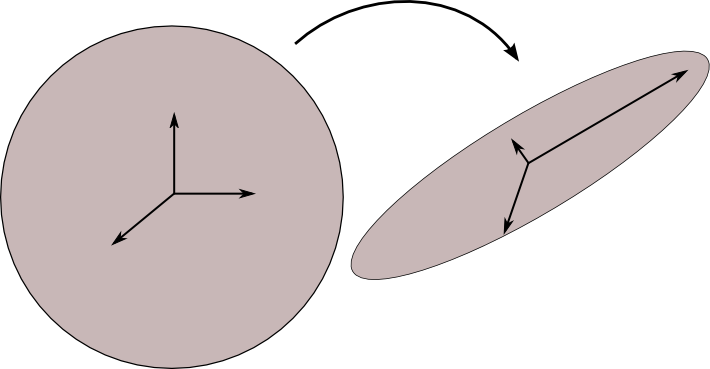
\includegraphics{phspace.png}
\caption{Schematyczna reprezentacja przestrzeni fazowej.}\end{figure}

Dwie trajektorię leżące początkowo blisko siebie propagują w czasie w odległości   $l(t)   \propto e^{\lambda_1 t}$, powierzchnia  $S$ zmienia się w tempie $S(t)  \propto e^{(\lambda_1 + \lambda_2) t}$, a objętość  $M$ zmienia się w tempie $M(t)  \propto e^{(\lambda_1 + \lambda_2 + \lambda_3) t}$. W reżimie chaotycznym co najmniej jeden z wykładników Lapunowa jest dodatni. Oznacza to, że w przestrzeni fazowej trajektorie rozbiegają się w jednym kierunku. Jeżeli wszystkie 3 wykładniki są ujemne, układ jest w rteżimie regularnum (periodycznym, quasi-periodycznym). Nie ma metod analitycznych pozwalających obliczyć wykładniki Lapunowa. Metody numeryczne też nie są proste. W literaturze można znaleźć algorytmy służące do wyznaczania $\lambda_1, \lambda_2, \lambda_3$.

W przypadku oscylatora Duffinga można otrzymać cząstkowe  informacje o wykładnikach Lapunowa.
\begin{enumerate}
\item {} 
Trzecie równanie dla pomocniczej zmiennej $z$ można rozwiązać otrzymując funkcję

\end{enumerate}
\begin{quote}
\phantomsection\label{ch2/chII012:equation-eqn8}\begin{gather}
\begin{split}z(t) = \omega t + c\end{split}\label{ch2/chII012-eqn8}
\end{gather}
Z pewnością dwie bliskie sobie trajektorie $z_1(t) = \omega t+c_1$ oraz $z_2(t) = \omega t + c_2$ dla chwili   $t=0$ nie rozbiegają się exponencjalnie ponieważ
\phantomsection\label{ch2/chII012:equation-eqn9}\begin{gather}
\begin{split}|z_1(t) - z_2(t)| = |c_1 -c_2|\end{split}\label{ch2/chII012-eqn9}
\end{gather}
Dlatego też jeden z wykładników wynosi zero, np.
\phantomsection\label{ch2/chII012:equation-eqn10}\begin{gather}
\begin{split}\lambda_2 = 0\end{split}\label{ch2/chII012-eqn10}
\end{gather}\end{quote}
\begin{enumerate}
\setcounter{enumi}{1}
\item {} 
Przypomnijmy w tym miejscu, że oscylator Duffinga jest opisany przez układ równań

\end{enumerate}
\begin{quote}
\phantomsection\label{ch2/chII012:equation-eqn11}\begin{gather}
\begin{split}\dot x = F_1 = y , \qquad x(0) = x_0,\end{split}\label{ch2/chII012-eqn11}\\\begin{split}\dot y = F_2 = x - x^3 -\gamma y + A \cos z , \qquad y(0) = y_0,\end{split}\notag\\\begin{split}z = F_3 = \omega, \qquad z(0) = 0.\end{split}\notag
\end{gather}
Zbadajmy, jak zmienia się w czasie objętość fazowa układu.  W tym celu musimy obliczyć dywergencję pola wektorowego
\phantomsection\label{ch2/chII012:equation-eqn12}\begin{gather}
\begin{split} div  \vec F = \frac{\partial F_1}{\partial x} + \frac{\partial F_2}{\partial y} + \frac{\partial F_3}{\partial z}  = -\gamma < 0\end{split}\label{ch2/chII012-eqn12}
\end{gather}
Oznacza to, że objętość fazowa w przestrzeni 3-wymiarowej maleje w tempie (zobacz paragraf o układach dysypatywnych)
\phantomsection\label{ch2/chII012:equation-eqn13}\begin{gather}
\begin{split}M(t) \propto e^{-\gamma t}\end{split}\label{ch2/chII012-eqn13}
\end{gather}\end{quote}

Z drugiej strony, jak powiedzieliśmy powyżej,
\phantomsection\label{ch2/chII012:equation-eqn14}\begin{gather}
\begin{split}M(t)  \propto e^{(\lambda_1 + \lambda_2 + \lambda_3) t}\end{split}\label{ch2/chII012-eqn14}
\end{gather}
Wynika stąd, że suma wszystkich wykładników jest stała i wynosi
\phantomsection\label{ch2/chII012:equation-eqn15}\begin{gather}
\begin{split}\lambda_1 + \lambda_2 + \lambda_3 = -\gamma  <  0\end{split}\label{ch2/chII012-eqn15}
\end{gather}
czyli tylko stała tłumienia $\gamma$ określa tempo malenia objętości fazowej.  Ponieważ $\lambda_2 =0$, otrzymujemy interesujący związek pomiędzy dwoma pozostałymi wykładnikami:
\phantomsection\label{ch2/chII012:equation-eqn16}\begin{gather}
\begin{split}\lambda_1 + \lambda_3 = -\gamma\end{split}\label{ch2/chII012-eqn16}
\end{gather}
W reżimie chaotycznym jeden z wykładników jest dodatni, np. $\lambda_1 >0$ oraz drugi wykładnik musi być ujemny, np. $\lambda_3 < 0$.  Mamy obecnie następujące informacje o wykładnikach Lapunowa dla oscylatora  Duffinga:
\phantomsection\label{ch2/chII012:equation-eqn17}\begin{gather}
\begin{split}\lambda_1  >  \lambda_2  >  \lambda_3, \qquad   \lambda_1 > 0, \qquad \lambda_2  = 0, \qquad   \lambda_3 < 0,  \qquad M(t) =  M(0)  e^{(\lambda_1 + \lambda_2 + \lambda_3) t} = M(0) e^{-\gamma t}\end{split}\label{ch2/chII012-eqn17}
\end{gather}
Zwracamy uwgę na to, że elipsoida  w 3-wymiarowej przestrzeni fazowej rozciąga się w jednym kierunku, kurczy się w drugim kierunku i nie zmienia się w trzecim kierunku  oraz objętość elipsoidy cały czas maleje.Tak to wygląda w reżimie chaotycznym. W reżimie nie-chaotycznym: elipsoida kurczy się  w jednym kierunku, kurczy się w drugim kierunku i nie zmienia się w trzecim kierunku  oraz objętość elipsoidy cały czas maleje. Atraktory, które pokazywaliśmy poprzednio, istnieją w 3-wymiarowej przestrzeni fazowej, ale ponieważ objętość fazowa cały czas maleje, wymiar atraktorów musi być mniejszy od 3. W reżimie nie-chaotycznym, n-okresowe atraktory  (krzywe) mają wymiar 1. Atraktory w reżimie chaotycznym mają wymiar większy niż 1, ale mniejszy niż 3. Kaplana i  Yorke (1979) postawili  hipotezę, że  istnieje związek pomiędzy wymiarem fraktalnym atraktora $D_A$  a wykładnikami Lapunowa. Relacja ta ma postać:
\phantomsection\label{ch2/chII012:equation-eqn18}\begin{gather}
\begin{split} D_A = 2 +  \frac{\lambda_1}{|\lambda_3|}  >  2\end{split}\label{ch2/chII012-eqn18}
\end{gather}
Jeżeli analizujemy wymiar atraktora w odwzorowaniu Poincarego (na płaszczyźnie), to wymiar ten jest o 1 mniejszy:
\phantomsection\label{ch2/chII012:equation-eqn19}\begin{gather}
\begin{split}d_A = D_A -1\end{split}\label{ch2/chII012-eqn19}
\end{gather}
Do dzisiaj jest to tylko hipoteza, choć w wielu przypadkach potwierdzona przez eksperymenty numeryczne.


\subsection{Widmo mocy}
\label{ch2/chII012:widmo-mocy}
Jest to kolejna wielkość, która może być indykatorem chaotycznego zachowania sie układu deterministycznego. Pojęcie widma mocy jest dobrze ugruntowane w teorii sygnałów, traktowanych jako nośnik informacji. W ogólności sygnały mogą być deterministyczne (jak w naszym przypadku) i losowe (stochastyczne). W sensie inżynierskim, sygnał to dowolna funkcja czasu.  Jako modele sygnałów wprowadza się również wielkości nazywane dystrybucjami (funkcjami uogólnionymi). Tylko  nieliczne proste sygnały można opisać formułami matematycznymi.  Większość sygnałów, z jakimi spotykamy się w praktyce, ma przebieg na tyle złożony i nieregularny, że ich bezpośredni opis  jako funkcji czasu jest kłopotliwy.  Dlatego też należy posługugiwać się  ich różnego rodzaju reprezentacjami. Reprezentacja sygnału stanowi pewien rodzaj jego symbolicznego opisu, niekiedy o znacznym stopniu abstrakcji. Jej istotą jest to, że zawiera ona pełną informację o sygnale, choć zwykle wyrażoną w innym języku, niż bezpośredni język  w terminach funkcji czasu.  Oznacza to, że znając sygnał, możemy jednoznacznie wyznaczyć jego reprezentację, znając zaś tę reprezentację – odtworzyć jednoznacznie sygnał. Istnieje wiele sposobów reprezentacji sygnałów. Jednym z nich jest analiza furierowska za pomocą transformat Fouriera lub szeregów Fouriera.

Przypomnijmy pojęcie transformacji Fouriera funkcji lub dystrybucji. W najprostszym ujęciu transformatą  Fouriera ${\hat f}(\omega)$  funkcji $f(t)$ nazywamy całkę
\phantomsection\label{ch2/chII012:equation-eqn20}\begin{gather}
\begin{split}{\hat f}(\omega) = \int_{-\infty}^{\; \infty}  \mbox{e}^{i \omega t} f(t)  dt\end{split}\label{ch2/chII012-eqn20}
\end{gather}
gdzie $\omega$ jest dowolną liczbą rzeczywistą.

Ponieważ nas interesuje ewolucja sygnału czasowego $f(t) = (x(t),  y(t),  z(t), ...)$ dla czasów $t>0$, zdefiniujemy nieco inaczej transformatę  Fouriera  jako graniczną wartość całki:
\phantomsection\label{ch2/chII012:equation-eqn21}\begin{gather}
\begin{split}{\hat f}(\omega) = \lim_{T\to\infty}  \; \int_{0}^{\; T}  \mbox{e}^{i \omega t} f(t)  dt\end{split}\label{ch2/chII012-eqn21}
\end{gather}
W praktyce obliczeń komputerowych nigdy nie wykonujemy dokładnej granicy $T\to \infty$, ale rozpatrujemy dostatecznie długi czas, gdy pojawia się stan ustalony i efekty przejściowe w ewolucji zanikają.  Ze względu na występowanie funkcji  podcałkowej  :math:{}` mbox\{e\}\textasciicircum{}\{i omega t\}{}`, transformata Fouriera jest  funkcją  zespoloną. Dlatego też bada się funkcję rzeczywistą w postaci
\phantomsection\label{ch2/chII012:equation-eqn22}\begin{gather}
\begin{split}P(\omega) = \lvert {\hat f}(\omega) \rvert^2\end{split}\label{ch2/chII012-eqn22}
\end{gather}
Nazywa się ona widmem mocy sygnału czasowego $f(t)$. W pewnych przypadkach, faktycznie jest to wielkość fizyczna mająca interpretację mocy, a liczba  $\omega$ jest częstością, która jest wielkościa dodatnią, $\omega > 0$.  W dalszym ciągu przyjmiemy to założenie o dodatniości ``częstości''. W ogólności, jej związek z mocą ( w sensie fizycznym) jest luźny. To widmo mocy jest zdefiniowane inaczej niż w teorii stacjonarnych procesów stochastycznych: tam jest to transformacja Fouriera funkcji korelacyjnej $C(t)$  procesu stochastycznego.

Aby wyrobić sobie intuicję o własnościach transformaty Fouriera i widma mocy, wystarczy rozpatrzeć kilka  przypadków funkcji $f(t)$.
\begin{description}
\item[{Przypadek 1}] \leavevmode
Jedna harmonika  (fala monochromatyczna)
\phantomsection\label{ch2/chII012:equation-eqn23}\begin{gather}
\begin{split}f_1(t) = A \cos (\Omega t), \qquad {\hat f}_1(\omega) = A  \int_{0}^{\; \infty}  \mbox{e}^{i \omega t} \cos(\Omega t)  dt =\frac{\pi }{2}  A  \delta(\omega - \Omega)\end{split}\label{ch2/chII012-eqn23}
\end{gather}
Transformatą Fouriera jest delta Diraca $\delta$, czyli w widmie mocy pojawia się jeden pik (który w praktyce jest zawsze skończony).

\item[{Przypadek 2}] \leavevmode
Kilka harmonik
\phantomsection\label{ch2/chII012:equation-eqn24}\begin{gather}
\begin{split}f_2(t) = \sum_{k=1}^{n} A_k \cos (\Omega_k  t), \qquad {\hat f}_2(\omega) = \sum_{k=1}^{n} A_k  \int_{0}^{\; \infty}  \mbox{e}^{i \omega t} \cos(\Omega_k t)  dt = \frac{\pi}{2}  \sum_{k=1}^{n} A_k   \delta(\omega - \Omega_k)\end{split}\label{ch2/chII012-eqn24}
\end{gather}
Transformatą Fouriera jest suma przesuniętych delt Diraca $\delta$, czyli w widmie mocy pojawia się szereg  pików (które w praktyce są  zawsze skończone).

\end{description}

Zauważmy, że dla tak zdefiniowanych  transformacji Fouriera nie istnieje widmo mocy, ponieważ w ścisłym sensie matematycznym nie istnieje $\delta^2(\omega -\Omega)$ dla delty Diraca. Jednak nie chodzi o precyzję matematyczną, ale o to że pojawia się pik, który nigdy nie jest nieskończony jak w delcie Diraca. My jednak potrzebujemy praktycznej metody sprawdzania chaotyczności procesu i zwykle sygnał próbkujemy dla dyskretnych wartości czasu t. Dlatego też należy wykorzystać aparat Dyskretnej Transformacji Fouriera, która  skończony ciągu sygnału
\phantomsection\label{ch2/chII012:equation-eqn25}\begin{gather}
\begin{split}\{x_0, x_1, x_2, ..., x_{N-1}\}\end{split}\label{ch2/chII012-eqn25}
\end{gather}
przekształca w skończony ciąg amplitud
\phantomsection\label{ch2/chII012:equation-eqn26}\begin{gather}
\begin{split}\{A_0, A_1, A_2, ..., A_{N-1}\}\end{split}\label{ch2/chII012-eqn26}
\end{gather}
odpowiednich harmonik poprzez relacje:
\phantomsection\label{ch2/chII012:equation-eqn27}\begin{gather}
\begin{split}A_k = \sum_{n=0}^{N-1}  x_n  \mbox{e}^{- 2\pi i k n/N}, \qquad x_n = \frac{1}{N}  \sum_{k=0}^{N-1}  A_k  \mbox{e}^{2\pi i k n/N}\end{split}\label{ch2/chII012-eqn27}
\end{gather}
Dla odpowiednio dużej liczby $N$ (w praktyce rzędu 100), zgodność pomiędzy transformatą Fouriera a Dyskretną Transformatą Fouriera jest zadziwiająco dobra.

\begin{Verbatim}[commandchars=\\\{\}]
\PYG{n}{var}\PYG{p}{(}\PYG{l+s}{\PYGZsq{}}\PYG{l+s}{x y z}\PYG{l+s}{\PYGZsq{}}\PYG{p}{)}
\PYG{n}{g}\PYG{p}{,} \PYG{n}{w0} \PYG{o}{=} \PYG{l+m+mf}{0.5}\PYG{p}{,} \PYG{l+m+mi}{1}
\PYG{n}{x0}\PYG{p}{,} \PYG{n}{y0}\PYG{p}{,} \PYG{n}{z0} \PYG{o}{=} \PYG{l+m+mf}{0.1}\PYG{p}{,} \PYG{l+m+mf}{0.1}\PYG{p}{,} \PYG{l+m+mi}{0}

\PYG{n}{Aval} \PYG{o}{=} \PYG{p}{[}\PYG{l+m+mf}{0.325}\PYG{p}{,}\PYG{l+m+mf}{0.354}\PYG{p}{,}\PYG{l+m+mf}{0.357}\PYG{p}{,}\PYG{l+m+mf}{0.358}\PYG{p}{,}\PYG{l+m+mf}{0.4}\PYG{p}{]}
\PYG{n}{kolor} \PYG{o}{=} \PYG{p}{[}\PYG{l+s}{\PYGZsq{}}\PYG{l+s}{blue}\PYG{l+s}{\PYGZsq{}}\PYG{p}{,}\PYG{l+s}{\PYGZsq{}}\PYG{l+s}{red}\PYG{l+s}{\PYGZsq{}}\PYG{p}{,}\PYG{l+s}{\PYGZsq{}}\PYG{l+s}{green}\PYG{l+s}{\PYGZsq{}}\PYG{p}{,}\PYG{l+s}{\PYGZsq{}}\PYG{l+s}{black}\PYG{l+s}{\PYGZsq{}}\PYG{p}{,}\PYG{l+s}{\PYGZsq{}}\PYG{l+s}{orange}\PYG{l+s}{\PYGZsq{}}\PYG{p}{]}
\PYG{n}{p} \PYG{o}{=} \PYG{p}{[}\PYG{p}{]}

\PYG{n}{j} \PYG{o}{=} \PYG{l+m+mi}{0}
\PYG{k}{for} \PYG{n}{a} \PYG{o+ow}{in} \PYG{n}{Aval}\PYG{p}{:}
    \PYG{n}{dx} \PYG{o}{=} \PYG{n}{y}
    \PYG{n}{dy} \PYG{o}{=} \PYG{n}{x} \PYG{o}{\PYGZhy{}} \PYG{n}{x}\PYG{o}{*}\PYG{o}{*}\PYG{l+m+mi}{3} \PYG{o}{\PYGZhy{}} \PYG{n}{g}\PYG{o}{*}\PYG{n}{y} \PYG{o}{+} \PYG{n}{a}\PYG{o}{*}\PYG{n}{cos}\PYG{p}{(}\PYG{n}{z}\PYG{p}{)}
    \PYG{n}{dz} \PYG{o}{=} \PYG{n}{w0}

    \PYG{n}{h} \PYG{o}{=} \PYG{l+m+mf}{0.1}
    \PYG{n}{T} \PYG{o}{=} \PYG{l+m+mi}{1100}
    \PYG{n}{skip} \PYG{o}{=} \PYG{l+m+mi}{100}
    \PYG{n}{iskip} \PYG{o}{=} \PYG{n+nb}{int}\PYG{p}{(}\PYG{n}{skip}\PYG{o}{/}\PYG{n}{h}\PYG{p}{)}
    \PYG{n}{listT} \PYG{o}{=} \PYG{n}{srange}\PYG{p}{(}\PYG{l+m+mi}{0}\PYG{p}{,}\PYG{n}{T}\PYG{p}{,}\PYG{n}{h}\PYG{p}{,} \PYG{n}{include\PYGZus{}endpoint}\PYG{o}{=}\PYG{l+m+mi}{0}\PYG{p}{)}
    \PYG{n}{num} \PYG{o}{=} \PYG{n}{desolve\PYGZus{}odeint}\PYG{p}{(}\PYG{n}{vector}\PYG{p}{(}\PYG{p}{[}\PYG{n}{dx}\PYG{p}{,} \PYG{n}{dy}\PYG{p}{,} \PYG{n}{dz}\PYG{p}{]}\PYG{p}{)}\PYG{p}{,} \PYG{p}{[}\PYG{n}{x0}\PYG{p}{,} \PYG{n}{y0}\PYG{p}{,} \PYG{n}{z0}\PYG{p}{]}\PYG{p}{,} \PYG{n}{listT}\PYG{p}{,} \PYG{p}{[}\PYG{n}{x}\PYG{p}{,}\PYG{n}{y}\PYG{p}{,}\PYG{n}{z}\PYG{p}{]}\PYG{p}{)}
    \PYG{n}{iks} \PYG{o}{=} \PYG{n}{num}\PYG{p}{[}\PYG{p}{:}\PYG{p}{,}\PYG{l+m+mi}{0}\PYG{p}{]}\PYG{o}{.}\PYG{n}{tolist}\PYG{p}{(}\PYG{p}{)}\PYG{p}{[}\PYG{n}{iskip}\PYG{p}{:}\PYG{p}{]}

    \PYG{n}{freq} \PYG{o}{=} \PYG{p}{[}\PYG{n}{i}\PYG{o}{/}\PYG{p}{(}\PYG{n}{T}\PYG{o}{\PYGZhy{}}\PYG{n}{skip}\PYG{p}{)} \PYG{k}{for} \PYG{n}{i} \PYG{o+ow}{in} \PYG{n+nb}{range}\PYG{p}{(}\PYG{n+nb}{len}\PYG{p}{(}\PYG{n}{iks}\PYG{p}{)}\PYG{o}{/}\PYG{l+m+mi}{2}\PYG{p}{)}\PYG{p}{]} \PYG{o}{+}\PYGZbs{}
           \PYG{p}{[}\PYG{o}{\PYGZhy{}}\PYG{n+nb}{len}\PYG{p}{(}\PYG{n}{iks}\PYG{p}{)}\PYG{o}{/}\PYG{p}{(}\PYG{n}{T}\PYG{o}{\PYGZhy{}}\PYG{n}{skip}\PYG{p}{)} \PYG{o}{+} \PYG{n}{i}\PYG{o}{/}\PYG{p}{(}\PYG{n}{T}\PYG{o}{\PYGZhy{}}\PYG{n}{skip}\PYG{p}{)} \PYG{k}{for} \PYG{n}{i} \PYG{o+ow}{in} \PYG{n+nb}{range}\PYG{p}{(}\PYG{n+nb}{len}\PYG{p}{(}\PYG{n}{iks}\PYG{p}{)}\PYG{o}{/}\PYG{l+m+mi}{2}\PYG{p}{,}\PYG{n+nb}{len}\PYG{p}{(}\PYG{n}{iks}\PYG{p}{)}\PYG{p}{)}\PYG{p}{]}
    \PYG{n}{freq} \PYG{o}{=} \PYG{p}{[}\PYG{n}{f}\PYG{o}{*}\PYG{l+m+mf}{2.}\PYG{o}{*}\PYG{n}{n}\PYG{p}{(}\PYG{n}{pi}\PYG{p}{)}\PYG{o}{/}\PYG{n}{w0} \PYG{k}{for} \PYG{n}{f} \PYG{o+ow}{in} \PYG{n}{freq}\PYG{p}{]}

    \PYG{n}{vx} \PYG{o}{=} \PYG{n}{vector}\PYG{p}{(}\PYG{n}{iks}\PYG{p}{)}
    \PYG{n}{A} \PYG{o}{=} \PYG{n}{vx}\PYG{o}{.}\PYG{n}{fft}\PYG{p}{(}\PYG{p}{)}\PYG{o}{.}\PYG{n}{apply\PYGZus{}map}\PYG{p}{(}\PYG{k}{lambda} \PYG{n}{x}\PYG{p}{:}\PYG{n}{x}\PYG{o}{.}\PYG{n}{abs2}\PYG{p}{(}\PYG{p}{)}\PYG{p}{)}
    \PYG{n}{p}\PYG{o}{.}\PYG{n}{append}\PYG{p}{(}\PYG{n}{list\PYGZus{}plot}\PYG{p}{(}\PYG{n+nb}{zip}\PYG{p}{(}\PYG{n}{freq}\PYG{p}{,}\PYG{n}{A}\PYG{o}{.}\PYG{n}{apply\PYGZus{}map}\PYG{p}{(}\PYG{k}{lambda} \PYG{n}{x}\PYG{p}{:}\PYG{n}{x}\PYG{o}{.}\PYG{n}{log}\PYG{p}{(}\PYG{p}{)}\PYG{p}{)}\PYG{p}{)}\PYG{p}{)}\PYG{p}{)}

    \PYG{n}{j} \PYG{o}{+}\PYG{o}{=} \PYG{l+m+mi}{1}
\end{Verbatim}


\subsection{Funkcja korelacyjna}
\label{ch2/chII012:funkcja-korelacyjna}
Jeżeli badamy deterministyczny proces, nie zawsze jest sens mówić o wartości średniej,  w takim sensie jak w teorii procesów stochastycznych lub na wykładach z fizyki statystycznej: średniowanie po realizacjach lub po zespole statystycznym . Ale jeżeli proces deterministyczny jest ergodyczny (trudne pojęcie!), to średnia wartość jest dobrze określona i średnia po zespole  jest równoważna średniej po czasie.  Jeżeli dodatkowo  proces jest stacjonarny, to można zdefiniować funkcję korelacyjną $C(\tau)$  dla procesu deterministycznego. W naszym przypadku: dla położenia lub prędkości, jest ona zdefiniowana przez relacje:
\phantomsection\label{ch2/chII012:equation-eqn28}\begin{gather}
\begin{split}C(\tau) = \lim_{T\to \infty}   \frac{1}{T}   \int_0^{\; T}  [x(t+\tau) - \langle x(t+\tau)\rangle]  [ x(t) - \langle x(t)\rangle]  dt, \qquad \langle x(t)\rangle = \lim_{T\to \infty}   \frac{1}{T}   \int_0^{\; T}   x(t)  dt\end{split}\label{ch2/chII012-eqn28}
\end{gather}
Jeżeli mamy rozwiązanie równania ruchu $x(t)$, to w zależności od postaci tego rozwiązania również SAGE poradzi sobie z rozwiązaniem całki. Jeżeli analityczny wzór będzie poza możliwościami obliczeń symbolicznych, zawsze możemy wygenerować sobie szereg czasowy $x = \{x_1, x_2, \dots \}$. Realizacja funkcji korelacyjnej w SAGE nie będzie stanowić problemu numerycznego. Możemy pokusić się o samodzielne sformułowanie problemu, lub skorzystać z metod pakietu \code{finance}.

\begin{Verbatim}[commandchars=\\\{\}]
\PYG{k}{def} \PYG{n+nf}{korelator}\PYG{p}{(}\PYG{n}{dane}\PYG{p}{,} \PYG{n}{tau}\PYG{o}{=}\PYG{l+m+mi}{0}\PYG{p}{)}\PYG{p}{:}
    \PYG{n}{ret} \PYG{o}{=} \PYG{n+nb+bp}{None}
    \PYG{k}{if} \PYG{n}{tau} \PYG{o}{==} \PYG{l+m+mi}{0}\PYG{p}{:}
        \PYG{k}{return} \PYG{l+m+mi}{1}
    \PYG{k}{else}\PYG{p}{:}
        \PYG{n}{tau} \PYG{o}{=} \PYG{n+nb}{abs}\PYG{p}{(}\PYG{n}{tau}\PYG{p}{)}
        \PYG{n}{m} \PYG{o}{=} \PYG{n}{mean}\PYG{p}{(}\PYG{n}{dane}\PYG{p}{)}
        \PYG{n}{dane} \PYG{o}{=} \PYG{p}{[}\PYG{n}{dane}\PYG{p}{[}\PYG{n}{i}\PYG{p}{]} \PYG{o}{\PYGZhy{}} \PYG{n}{m} \PYG{k}{for} \PYG{n}{i} \PYG{o+ow}{in} \PYG{n+nb}{xrange}\PYG{p}{(}\PYG{n+nb}{len}\PYG{p}{(}\PYG{n}{dane}\PYG{p}{)}\PYG{p}{)}\PYG{p}{]}
        \PYG{n}{v} \PYG{o}{=} \PYG{n}{vector}\PYG{p}{(}\PYG{n}{dane}\PYG{p}{)}
        \PYG{n}{sigma} \PYG{o}{=} \PYG{n}{v}\PYG{o}{.}\PYG{n}{dot\PYGZus{}product}\PYG{p}{(}\PYG{n}{v}\PYG{p}{)}
        \PYG{k}{if} \PYG{n}{tau} \PYG{o}{\PYGZlt{}} \PYG{n+nb}{len}\PYG{p}{(}\PYG{n}{dane}\PYG{p}{)}\PYG{p}{:}
            \PYG{n}{ret} \PYG{o}{=} \PYG{n}{v}\PYG{p}{[}\PYG{p}{:}\PYG{o}{\PYGZhy{}}\PYG{n}{tau}\PYG{p}{]}\PYG{o}{.}\PYG{n}{dot\PYGZus{}product}\PYG{p}{(}\PYG{n}{v}\PYG{p}{[}\PYG{n}{tau}\PYG{p}{:}\PYG{p}{]}\PYG{p}{)}
        \PYG{n}{ret} \PYG{o}{/}\PYG{o}{=} \PYG{n}{sigma}
    \PYG{k}{return} \PYG{n}{ret}
\end{Verbatim}

Teraz obliczymy sobie ową funkcję korelacji dla oscylatora Duffinga.

\begin{Verbatim}[commandchars=\\\{\}]
\PYG{n}{var}\PYG{p}{(}\PYG{l+s}{\PYGZsq{}}\PYG{l+s}{x y z}\PYG{l+s}{\PYGZsq{}}\PYG{p}{)}
\PYG{n}{a}\PYG{p}{,} \PYG{n}{g}\PYG{p}{,} \PYG{n}{w0} \PYG{o}{=} \PYG{l+m+mf}{0.3}\PYG{p}{,} \PYG{l+m+mf}{0.26}\PYG{p}{,} \PYG{l+m+mi}{1}
\PYG{n}{x0}\PYG{p}{,} \PYG{n}{y0}\PYG{p}{,} \PYG{n}{z0} \PYG{o}{=} \PYG{l+m+mf}{0.1}\PYG{p}{,} \PYG{l+m+mf}{0.1}\PYG{p}{,} \PYG{l+m+mi}{0}

\PYG{n}{dx} \PYG{o}{=} \PYG{n}{y}
\PYG{n}{dy} \PYG{o}{=} \PYG{n}{x} \PYG{o}{\PYGZhy{}} \PYG{n}{x}\PYG{o}{*}\PYG{o}{*}\PYG{l+m+mi}{3} \PYG{o}{\PYGZhy{}} \PYG{n}{g}\PYG{o}{*}\PYG{n}{y} \PYG{o}{+} \PYG{n}{a}\PYG{o}{*}\PYG{n}{cos}\PYG{p}{(}\PYG{n}{z}\PYG{p}{)}
\PYG{n}{dz} \PYG{o}{=} \PYG{n}{w0}

\PYG{n}{h} \PYG{o}{=} \PYG{l+m+mf}{0.1}
\PYG{n}{T} \PYG{o}{=} \PYG{l+m+mi}{1000}
\PYG{n}{listT} \PYG{o}{=} \PYG{n}{srange}\PYG{p}{(}\PYG{l+m+mi}{0}\PYG{p}{,}\PYG{n}{T}\PYG{p}{,}\PYG{n+nb}{float}\PYG{p}{(}\PYG{n}{h}\PYG{p}{)}\PYG{p}{,} \PYG{n}{include\PYGZus{}endpoint}\PYG{o}{=}\PYG{n+nb+bp}{True}\PYG{p}{)}
\PYG{n}{num} \PYG{o}{=} \PYG{n}{desolve\PYGZus{}odeint}\PYG{p}{(}\PYG{n}{vector}\PYG{p}{(}\PYG{p}{[}\PYG{n}{dx}\PYG{p}{,} \PYG{n}{dy}\PYG{p}{,} \PYG{n}{dz}\PYG{p}{]}\PYG{p}{)}\PYG{p}{,} \PYG{p}{[}\PYG{n}{x0}\PYG{p}{,} \PYG{n}{y0}\PYG{p}{,} \PYG{n}{z0}\PYG{p}{]}\PYG{p}{,} \PYG{n}{listT}\PYG{p}{,} \PYG{p}{[}\PYG{n}{x}\PYG{p}{,}\PYG{n}{y}\PYG{p}{,}\PYG{n}{z}\PYG{p}{]}\PYG{p}{)}
\end{Verbatim}

Skorzystamy zarówno z naszej funkcji jak i z wbudowanego w SAGE pakietu \code{finance},
obliczając funkcję (auto)korelacji dla położenia i dla prędkości.

\begin{Verbatim}[commandchars=\\\{\}]
\PYG{c}{\PYGZsh{}x}
\PYG{n}{dane} \PYG{o}{=} \PYG{n}{num}\PYG{p}{[}\PYG{p}{:}\PYG{p}{,}\PYG{l+m+mi}{0}\PYG{p}{]}\PYG{o}{.}\PYG{n}{tolist}\PYG{p}{(}\PYG{p}{)}

\PYG{c}{\PYGZsh{} nasz korelator}
\PYG{n}{my\PYGZus{}acorr} \PYG{o}{=} \PYG{p}{[}\PYG{n}{korelator}\PYG{p}{(}\PYG{n}{dane}\PYG{p}{,}\PYG{n}{i}\PYG{o}{*}\PYG{l+m+mi}{10}\PYG{p}{)} \PYG{k}{for} \PYG{n}{i} \PYG{o+ow}{in} \PYG{n+nb}{range}\PYG{p}{(}\PYG{l+m+mi}{33}\PYG{p}{)}\PYG{p}{]}

\PYG{c}{\PYGZsh{} funkcja SAGE}
\PYG{n}{v} \PYG{o}{=} \PYG{n}{finance}\PYG{o}{.}\PYG{n}{TimeSeries}\PYG{p}{(}\PYG{n}{dane}\PYG{p}{)}
\PYG{n}{sage\PYGZus{}acorr} \PYG{o}{=} \PYG{p}{[}\PYG{n}{v}\PYG{o}{.}\PYG{n}{autocorrelation}\PYG{p}{(}\PYG{n}{i}\PYG{o}{*}\PYG{l+m+mi}{10}\PYG{p}{)} \PYG{k}{for} \PYG{n}{i} \PYG{o+ow}{in} \PYG{n+nb}{range}\PYG{p}{(}\PYG{l+m+mi}{33}\PYG{p}{)}\PYG{p}{]}
\end{Verbatim}

Powyższe rachunki możemy powtórzyć dla wszystkich punktów o których była mowa przy omawianiu bifurkacji.

\begin{Verbatim}[commandchars=\\\{\}]
\PYG{n}{var}\PYG{p}{(}\PYG{l+s}{\PYGZsq{}}\PYG{l+s}{x y z}\PYG{l+s}{\PYGZsq{}}\PYG{p}{)}
\PYG{n}{g}\PYG{p}{,} \PYG{n}{w0} \PYG{o}{=} \PYG{l+m+mf}{0.5}\PYG{p}{,} \PYG{l+m+mi}{1}
\PYG{n}{x0}\PYG{p}{,} \PYG{n}{y0}\PYG{p}{,} \PYG{n}{z0} \PYG{o}{=} \PYG{l+m+mf}{0.1}\PYG{p}{,} \PYG{l+m+mf}{0.1}\PYG{p}{,} \PYG{l+m+mi}{0}

\PYG{n}{Aval} \PYG{o}{=} \PYG{p}{[}\PYG{l+m+mf}{0.325}\PYG{p}{,}\PYG{l+m+mf}{0.354}\PYG{p}{,}\PYG{l+m+mf}{0.357}\PYG{p}{,}\PYG{l+m+mf}{0.358}\PYG{p}{,}\PYG{l+m+mf}{0.4}\PYG{p}{]}
\PYG{n}{p}\PYG{p}{,} \PYG{n}{ps} \PYG{o}{=} \PYG{p}{[}\PYG{p}{]}\PYG{p}{,} \PYG{p}{[}\PYG{p}{]}
\PYG{n}{kolor} \PYG{o}{=} \PYG{p}{[}\PYG{l+s}{\PYGZsq{}}\PYG{l+s}{blue}\PYG{l+s}{\PYGZsq{}}\PYG{p}{,}\PYG{l+s}{\PYGZsq{}}\PYG{l+s}{red}\PYG{l+s}{\PYGZsq{}}\PYG{p}{,}\PYG{l+s}{\PYGZsq{}}\PYG{l+s}{green}\PYG{l+s}{\PYGZsq{}}\PYG{p}{,}\PYG{l+s}{\PYGZsq{}}\PYG{l+s}{black}\PYG{l+s}{\PYGZsq{}}\PYG{p}{,}\PYG{l+s}{\PYGZsq{}}\PYG{l+s}{orange}\PYG{l+s}{\PYGZsq{}}\PYG{p}{]}
\PYG{n}{j} \PYG{o}{=} \PYG{l+m+mi}{0}
\PYG{k}{for} \PYG{n}{a} \PYG{o+ow}{in} \PYG{n}{Aval}\PYG{p}{:}
    \PYG{n}{dx} \PYG{o}{=} \PYG{n}{y}
    \PYG{n}{dy} \PYG{o}{=} \PYG{n}{x} \PYG{o}{\PYGZhy{}} \PYG{n}{x}\PYG{o}{*}\PYG{o}{*}\PYG{l+m+mi}{3} \PYG{o}{\PYGZhy{}} \PYG{n}{g}\PYG{o}{*}\PYG{n}{y} \PYG{o}{+} \PYG{n}{a}\PYG{o}{*}\PYG{n}{cos}\PYG{p}{(}\PYG{n}{z}\PYG{p}{)}
    \PYG{n}{dz} \PYG{o}{=} \PYG{n}{w0}

    \PYG{n}{h} \PYG{o}{=} \PYG{l+m+mf}{0.1}
    \PYG{n}{T} \PYG{o}{=} \PYG{l+m+mi}{2000}
    \PYG{n}{listT} \PYG{o}{=} \PYG{n}{srange}\PYG{p}{(}\PYG{l+m+mi}{0}\PYG{p}{,}\PYG{n}{T}\PYG{p}{,}\PYG{n}{h}\PYG{p}{,} \PYG{n}{include\PYGZus{}endpoint}\PYG{o}{=}\PYG{n+nb+bp}{True}\PYG{p}{)}
    \PYG{n}{num} \PYG{o}{=} \PYG{n}{desolve\PYGZus{}odeint}\PYG{p}{(}\PYG{n}{vector}\PYG{p}{(}\PYG{p}{[}\PYG{n}{dx}\PYG{p}{,} \PYG{n}{dy}\PYG{p}{,} \PYG{n}{dz}\PYG{p}{]}\PYG{p}{)}\PYG{p}{,} \PYG{p}{[}\PYG{n}{x0}\PYG{p}{,} \PYG{n}{y0}\PYG{p}{,} \PYG{n}{z0}\PYG{p}{]}\PYG{p}{,} \PYG{n}{listT}\PYG{p}{,} \PYG{p}{[}\PYG{n}{x}\PYG{p}{,}\PYG{n}{y}\PYG{p}{,}\PYG{n}{z}\PYG{p}{]}\PYG{p}{)}

    \PYG{n}{d} \PYG{o}{=} \PYG{p}{(}\PYG{n}{num}\PYG{p}{[}\PYG{p}{:}\PYG{p}{,}\PYG{l+m+mi}{0}\PYG{p}{]}\PYG{o}{\PYGZhy{}}\PYG{n}{mean}\PYG{p}{(}\PYG{n}{num}\PYG{p}{[}\PYG{p}{:}\PYG{p}{,}\PYG{l+m+mi}{0}\PYG{p}{]}\PYG{p}{)}\PYG{p}{)}\PYG{o}{.}\PYG{n}{tolist}\PYG{p}{(}\PYG{p}{)}
    \PYG{n}{v} \PYG{o}{=} \PYG{n}{finance}\PYG{o}{.}\PYG{n}{TimeSeries}\PYG{p}{(}\PYG{n}{d}\PYG{p}{)}
    \PYG{n}{kor} \PYG{o}{=} \PYG{p}{[}\PYG{n}{v}\PYG{o}{.}\PYG{n}{autocorrelation}\PYG{p}{(}\PYG{n}{i}\PYG{o}{*}\PYG{l+m+mi}{5}\PYG{p}{)} \PYG{k}{for} \PYG{n}{i} \PYG{o+ow}{in} \PYG{n+nb}{range}\PYG{p}{(}\PYG{n+nb}{len}\PYG{p}{(}\PYG{n}{d}\PYG{p}{)}\PYG{o}{/}\PYG{l+m+mi}{5}\PYG{p}{)}\PYG{p}{]}
    \PYG{n}{p}\PYG{o}{.}\PYG{n}{append}\PYG{p}{(}\PYG{n}{list\PYGZus{}plot}\PYG{p}{(}\PYG{n}{kor}\PYG{p}{,} \PYG{n}{plotjoined}\PYG{o}{=}\PYG{l+m+mi}{1}\PYG{p}{,} \PYG{n}{color}\PYG{o}{=}\PYG{n}{kolor}\PYG{p}{[}\PYG{n}{j}\PYG{p}{]}\PYG{p}{,} \PYG{n}{legend\PYGZus{}label}\PYG{o}{=}\PYG{l+s}{r\PYGZdq{}}\PYG{l+s}{\PYGZdl{}a = }\PYG{l+s+si}{\PYGZpc{}.3f}\PYG{l+s}{\PYGZdl{}}\PYG{l+s}{\PYGZdq{}}\PYG{o}{\PYGZpc{}}\PYG{n}{a}\PYG{p}{)}\PYG{p}{)}
    \PYG{n}{ps}\PYG{o}{.}\PYG{n}{append}\PYG{p}{(}\PYG{n}{list\PYGZus{}plot}\PYG{p}{(}\PYG{n}{kor}\PYG{p}{[}\PYG{p}{:}\PYG{n+nb}{len}\PYG{p}{(}\PYG{n}{kor}\PYG{p}{)}\PYG{o}{/}\PYG{l+m+mi}{20}\PYG{p}{]}\PYG{p}{,} \PYG{n}{plotjoined}\PYG{o}{=}\PYG{l+m+mi}{1}\PYG{p}{,} \PYG{n}{color}\PYG{o}{=}\PYG{n}{kolor}\PYG{p}{[}\PYG{n}{j}\PYG{p}{]}\PYG{p}{,} \PYG{n}{legend\PYGZus{}label}\PYG{o}{=}\PYG{l+s}{r\PYGZdq{}}\PYG{l+s}{\PYGZdl{}a = }\PYG{l+s+si}{\PYGZpc{}.3f}\PYG{l+s}{\PYGZdl{}}\PYG{l+s}{\PYGZdq{}}\PYG{o}{\PYGZpc{}}\PYG{n}{a}\PYG{p}{)}\PYG{p}{)}

    \PYG{c}{\PYGZsh{}list\PYGZus{}plot(zip(d,num[:,1].tolist()),plotjoined=1,color=\PYGZsq{}red\PYGZsq{}).show()}
    \PYG{n}{j} \PYG{o}{+}\PYG{o}{=} \PYG{l+m+mi}{1}
\end{Verbatim}


\subsection{Odwzorowanie (cięcie) Poincarego}
\label{ch2/chII012:odwzorowanie-ciecie-poincarego}
Odwzorowanie Poincarego jest innym przedstawieniem dynamiki układu.  Najprościej jest to wytłumaczyć na przykładzie oscylatora Duffinga. Jego przestrzeń fazowa jest 3-wymiarowa. Ruch w trzecim wymiarze jest jednostajny, $z(t) = \omega_0 t$. Rzut orbity na płaszczyznę  $(x, y)$ jest przedstawiony w postaci krzywych fazowych w poprzednich częściach książki.
\begin{figure}[htbp]
\centering
\capstart

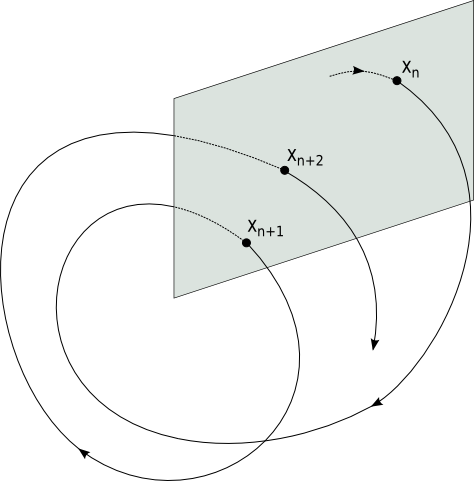
\includegraphics{poincare_section.png}
\caption{Konstrukcja cięcia Poincarego.}\end{figure}

Jak widać, we wszystkich przykładach krzywe fazowe na płaszczyźnie są ograniczone na pewnym obszarze $(x, y)$. We wszystkich rozpatrzywanych przypadach ruch wydaje sie być prawie-periodyczny: układ ciągle  powraca w te same obszary. Można zbudować następujące przedstawienie tego ruchu.

Okres siły periodycznej wynosi
\phantomsection\label{ch2/chII012:equation-eqn29}\begin{gather}
\begin{split}T = \frac{2\pi}{\omega_0}\end{split}\label{ch2/chII012-eqn29}
\end{gather}
Wprowadzamy dyskretny czas
\phantomsection\label{ch2/chII012:equation-eqn30}\begin{gather}
\begin{split}t_n = n T, \qquad n=1,  2,  3,  ...\end{split}\label{ch2/chII012-eqn30}
\end{gather}
Zapisujemy położenie i prędkość cząstki w dyskretnych chwilach czasu:
\phantomsection\label{ch2/chII012:equation-eqn31}\begin{gather}
\begin{split} x_n = x(t_n), \qquad y_n = y(t_n), \qquad x(0) = x_0, \qquad y(0) = y_0\end{split}\label{ch2/chII012-eqn31}
\end{gather}
Współrzędne tych punktów nanosimy na płaszczyznę. Otrzymujemy odwzorowanie które nazywamy odwzorowaniem Poincarego. Obrazowo mówiąc można w 3-wymiarowej przestrzeni fazowej wprowadzić płaszczyznę, tak aby nigdzie nie była styczna do trajektorii i była transwersalna do trajektorii (ściślej mówiąc do potoku fazowego), czyli aby trajektoria przecinała płaszczyznę, a nie była równoległa do niej (nie omijała jej).

Odwzorowanie Poincarego to przyporządkowanie:
\phantomsection\label{ch2/chII012:equation-eqn32}\begin{gather}
\begin{split}x_{n+1} = \mathcal{G}(x_n)\end{split}\label{ch2/chII012-eqn32}
\end{gather}
Jawna konstrukcja tego odwzorowania z wyjściowego układu równań  różniczkowych jest możliwa tylko w bardzo specjalnych przypadkach. W przypadku oscylatora Duffinga, nie można otrzymać jawnej postaci tego odwzorowania. Jedynie użycie komputera pozwala na graficzne przedstawienie funkcji $\mathcal{G}$.

Jakie wnioski płyną z takiego przedstawienia.
\begin{enumerate}
\item {} 
Gdyby trajektoria była krzywą zamkniętą w kształcie elipsy (atraktor o okresie 1) to na cięciu Poincarego otrzymalibyśmy 1 punkt:

\end{enumerate}
\begin{figure}[htbp]
\centering
\capstart

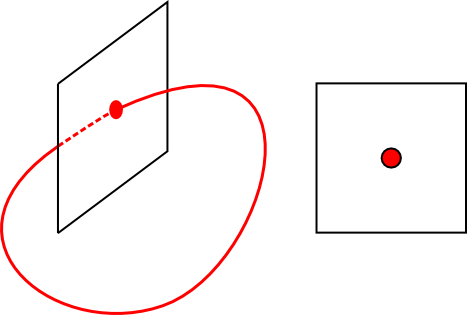
\includegraphics{poincare_period1.png}
\caption{Atraktor o okresie 1.}\end{figure}
\begin{enumerate}
\setcounter{enumi}{1}
\item {} 
Gdyby trajektoria była atraktorem  o okresie 2  to na cięciu Poincarego otrzymalibyśmy 2 punkty:

\end{enumerate}
\begin{figure}[htbp]
\centering
\capstart

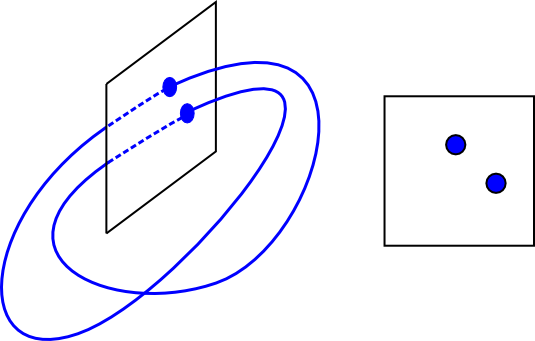
\includegraphics{poincare_period2.png}
\caption{Atraktor o okresie 2.}\end{figure}
\begin{enumerate}
\setcounter{enumi}{2}
\item {} 
Gdyby trajektoria była chaotyczna, to za każdym razem przebiega przez inne punkty płaszczyzny i tworzy zbiór składający sie z nieskończenie wielu punktów. Poniżej pokazano takie odwzorowanie dla oscylatora Duffinga.

\end{enumerate}
\begin{figure}[htbp]
\centering
\capstart

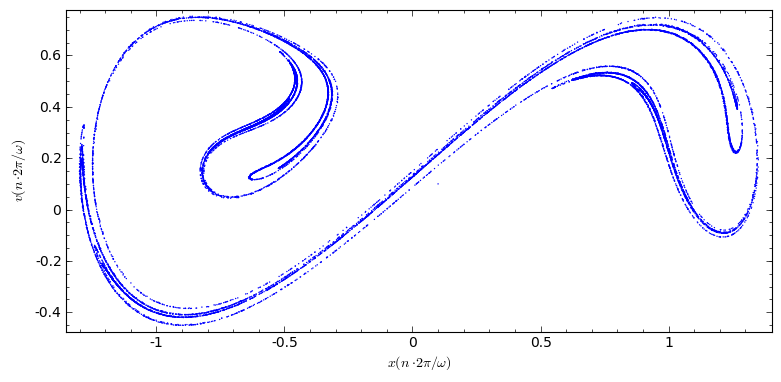
\includegraphics{chaotic_duffing.png}
\caption{Dziwny atraktor.}\end{figure}

Jeżeli jesteśmy w stanie zbudować graficznie przedstawienie Poincarego danego układu dynamicznego z ciągłym czasem, wówczas możemy rozpoznać takie reżimy które są ``podejrzane'' o własności chaotyczne.  Numerycznie nie powinno nastręczać to większych problemów. Jeżeli znamy $\omega_0$ bądź okres powrotu do obliczenia cięcia to wystarczy wykorzystać poniższy kod Sage. Zwracamy jedynie uwagę na to, że odpowiednio ``gęsty'' obraz uzyskamy dla bardzo długich przebiegów (dużych T).

\begin{Verbatim}[commandchars=\\\{\}]
\PYG{c}{\PYGZsh{} parametry układu równań różniczkowych}
\PYG{n}{a}\PYG{p}{,} \PYG{n}{g} \PYG{o}{=} \PYG{l+m+mf}{0.3}\PYG{p}{,} \PYG{l+m+mf}{0.26}

\PYG{c}{\PYGZsh{} częstotliwość (do obliczania cięcia Poincarego)}
\PYG{n}{w0} \PYG{o}{=} \PYG{l+m+mi}{1}

\PYG{c}{\PYGZsh{} wartości początkowe}
\PYG{n}{x0}\PYG{p}{,} \PYG{n}{y0}\PYG{p}{,} \PYG{n}{z0} \PYG{o}{=} \PYG{l+m+mf}{0.1}\PYG{p}{,} \PYG{l+m+mf}{0.1}\PYG{p}{,} \PYG{l+m+mi}{0}

\PYG{c}{\PYGZsh{}układ równań różniczkowych}
\PYG{n}{dx} \PYG{o}{=} \PYG{n}{y}
\PYG{n}{dy} \PYG{o}{=} \PYG{n}{x} \PYG{o}{\PYGZhy{}} \PYG{n}{x}\PYG{o}{*}\PYG{o}{*}\PYG{l+m+mi}{3} \PYG{o}{\PYGZhy{}} \PYG{n}{g}\PYG{o}{*}\PYG{n}{y} \PYG{o}{+} \PYG{n}{a}\PYG{o}{*}\PYG{n}{cos}\PYG{p}{(}\PYG{n}{z}\PYG{p}{)}
\PYG{n}{dz} \PYG{o}{=} \PYG{n}{w0}

\PYG{c}{\PYGZsh{}krok co jaki wypełniać się ma nasza lista}
\PYG{c}{\PYGZsh{}rozwiązań ustawiamy równy okresowi}
\PYG{n}{h} \PYG{o}{=} \PYG{l+m+mf}{2.0}\PYG{o}{*}\PYG{n}{pi}\PYG{o}{/}\PYG{n}{w0}

\PYG{c}{\PYGZsh{}\PYGZsh{}\PYGZsh{}}
\PYG{c}{\PYGZsh{}symulacje}
\PYG{c}{\PYGZsh{}\PYGZsh{}\PYGZsh{}}
\PYG{n}{T} \PYG{o}{=} \PYG{l+m+mi}{10000}
\PYG{n}{listT} \PYG{o}{=} \PYG{n}{srange}\PYG{p}{(}\PYG{l+m+mi}{0}\PYG{p}{,}\PYG{n}{T}\PYG{p}{,}\PYG{n+nb}{float}\PYG{p}{(}\PYG{n}{h}\PYG{p}{)}\PYG{p}{,} \PYG{n}{include\PYGZus{}endpoint}\PYG{o}{=}\PYG{n+nb+bp}{True}\PYG{p}{)}
\PYG{n}{sol} \PYG{o}{=} \PYG{n}{desolve\PYGZus{}odeint}\PYG{p}{(}\PYG{n}{vector}\PYG{p}{(}\PYG{p}{[}\PYG{n}{dx}\PYG{p}{,} \PYG{n}{dy}\PYG{p}{,} \PYG{n}{dz}\PYG{p}{]}\PYG{p}{)}\PYG{p}{,} \PYG{p}{[}\PYG{n}{x0}\PYG{p}{,} \PYG{n}{y0}\PYG{p}{,} \PYG{n}{z0}\PYG{p}{]}\PYG{p}{,} \PYG{n}{listT}\PYG{p}{,} \PYG{p}{[}\PYG{n}{x}\PYG{p}{,}\PYG{n}{y}\PYG{p}{,}\PYG{n}{z}\PYG{p}{]}\PYG{p}{)}
\end{Verbatim}


\subsection{Przykłady chaosu w Naturze}
\label{ch2/chII012:przyklady-chaosu-w-naturze}
Należy odróżnić procesy  chaotyczne  od procesów losowych. Procesy chaotyczne są deterministyczne, a procesy stochastyczne są procesami losowymi.  Procesy chaotyczne są badane przez matematyków, fizyków, chemików, biologów, socjologów, meteorologów, astrofizyków, w teorii informacji i neuronauce. We wszystkich tych gałęziach nauki, występują  deterministyczne modele wykazujące własności chaotyczne. Od lat 60-tych XX wieku opublikowano tysiące prac na temat układów chaotycznych.  Matematycy mówią, że prawie wszystkie układy dynamiczne są chaotyczne, a tylko nieliczne układy nie wykazują tej własności. Matematycy dowodzą, że przestrzeń fazowa układu modelowanego przez autonomiczny układ równań różniczkowych musi być co najmniej 3-wymiarowa, aby istniał chaos. Dla układów dyskretnych nie ma takich ograniczeń: jedno równanie  rekurencyjne $x_{n+1} = f(x_n)$  także wykazuje własności chaotyczne.

Poniżej podajemy kilka przykładów rzeczywistych zjawisk wykazujących własności chaotyczne.
\begin{enumerate}
\item {} 
Dynamika cieczy i turbulencja

\item {} 
Lasery

\item {} 
Układy elektroniczne

\item {} 
Plasma

\item {} 
Reakcje chemiczne

\end{enumerate}

Na stronie internetowej Wikipedii  z hasłem Chaos Theory  można znaleźć dalsze przykłady oraz podstawowe prace na ten temat. Na zakończenie tej części ksiązki musimy wspomnieć o człowieku, który to wszystko zapoczątkował w 1961 roku. Był to Edward Lorenz, matematyk i meteorolog amerykański,  który analizował jeden z najprostszych modeli pozwalających przewidywać pogodę. To z jego nazwiskiem związany jest  ``efekt motyla'' obrazujący niezwykłą czułość dynamiki na zaburzenia warunków  początkowych: czy ruch motyla w Brazylii może spowodować tornado w Teksasie (ściśle rzecz ujmując to Philip Merilees zasugerował  Lorenzowi taki tytuł wykładu podczas posiedzenia American Association for the Advancement of Science w 1972 roku). W tym obrazowym powiedzeniu zawarta jest istota chaosu: Motyl poprzez swój lot zaburza lokalnie ruch powietrza. Ten zaburzony ruch powietrza narasta i powoduje coraz to większe zmiany pogodowe, zmienia radykalnie ``trajektorię''  doprowadzając do tornada, które pojawi się nad Teksasem. Czy faktycznie motyl może być  taki groźny?


\chapter{Dynamika stochastyczna}
\label{index:id1}

\section{Równania stochastyczne i ich interpretacja}
\label{ch3/chIII011::doc}\label{ch3/chIII011:rownania-stochastyczne-i-ich-interpretacja}
Dotychczas rozważaliśmy modele deterministyczne bazujące na równaniach różniczkowych zwyczajnych. Twierdzenia matematyczne dają nam pewność że przy odpowiednicj założeniach rozwiązania równań różniczkowych są jednoznaczne przy zadanych warunkach początkowych. To jest kluczowe dla szerokiej klasy zjawisk w przyrodzie. Ten determinizm pozwala przewidywać ewolucję układów, pozwala konstruować i używać urządzenia, które pracują zgodnie z jego planowanymi funkcjami. To zapewniają twierdzenia matematyczne. Ale też pokazaliśmy, że matematyczny determinizm może być w praktyce złudny ponieważ dokładne w sensie matematycznym przygotowanie układu w określonych stanach początkowych jest niemożliwe. Niedokładności warunków początkowych mogą w trakcie ewolucji narastać powodując utratę przewidywalności ukrytą w równaniach różniczkowych. Dlatego ten fenomen nazywa się deterministycznym chaosem, czyli czymś co jest nieprzewidywalne ale jednocześnie nie jest losowe. Teraz rozpoczynamy wędrówkę po innej klasie zjawisk i procesów dynamicznych, a mianowicie po krainie procesów losowych. Ta klasa zjawisk bazuje na teorii procesów stochastycznych. To jest teoria matematyczna, której fundamenty oparte są o teorię prawdopodobieństwa. Niewątpliwie procesy stochastyczne nie są procesami deterministycznymi. Ich opis używa takich pojęć jak wartość średnia, fluktuacje czyli niespodziewane odchylania od wartości średniej, korelacja w różnych momentach czasu, charakterystyki spektralne ważne z eksperymentalnego punktu. Opis procesów stochastycznych jest do pewnego stopnia podobny do przedstawionego wcześniej opisu: bazuje on też na równaniach różniczkowych w których pojawiają się wyrażenia mogące przyjmować w sposób losowy różne wartości. Aby to wyjaśnić, posłużmy się przykładem z klasycznej mechaniki Newtona. Ba, możemy przywołać tu równanie Newtona dla cząstki o jednym stopniu swobody w potencjale $V(x)$. Jest ono postaci:
\phantomsection\label{ch3/chIII011:equation-eqn1}\begin{gather}
\begin{split}m \ddot x + \gamma \dot x = -V'(x)\end{split}\label{ch3/chIII011-eqn1}
\end{gather}
W równaniu tym pojawia się wyraz $\gamma \dot x$, który uwzględnia tarcie, tłumienie. Skąd pojawia się tarcie (tłumienie) w układzie? Wywodzi się ono z oddziaływania układu z otoczeniem. Rzeczywiste układy zawsze są w jakimś ośrodku: w powietrzu, wodzie, krysztale, komórce biologicznej. Owo oddziaływanie z otoczeniem jest źródłem tarcia, ale też jest jednym z czynników powodujących losowość. Wpływ otoczenia nie da się przewidzieć ponieważ rzeczywiste otoczenie składa się w bardzo dużej ilości cząstek. Przypomnijmy że w szkance wypełnionej wodą mamy około $10^{23}$ cząstek. Nie znamy ani położeń tych cząstek, ani prędkości tych cząstek. Ale gdybyśmy nawet znali te wielkości, to co nam z takiej wiedzy. Gdybyśmy chcieli modelować oddziaływanie układu z otoczeniem jako oddziaływanie opisane przez równania Newtona, to liczba równań Newtona rzędu $10^{23}$ jest przerażająco wielka. Nie bylibyśmy w stanie je zapisać, nie mówiąc o ich rozwiązywaniu. W tej beznadziejnej sytuacji powstaje fizyka statystyczna i teoria procesów stochastycznech. W tych teoriach nie ma determinizmu. Musi nam wystarczyć tylko prawdopodobieństwo tego, że cząstka w chwili $t=17$ znajduje się w jakimś obszarze $A$, że średnia wartość prędkośći w chwili $t=32 s$ wynosi $36 m/s$ oraz że cząstka średnio oddaliła się o $x=2 m$ od położenia początkowego.

W powyższym równaniu Newtona uwzględniliśmy wyraz opisujący tarcie (czyli oddziaływanie z otoczeniem), ale nie uwzględniliśmy jeszcze jednej siły, siły jaką cząstki otoczenia wywierają na układ. Poprawniejsze równanie miałoby postać:
\phantomsection\label{ch3/chIII011:equation-eqn2}\begin{gather}
\begin{split}m \ddot x + \gamma \dot x = -V'(x) + \Gamma (t) \qquad\end{split}\label{ch3/chIII011-eqn2}
\end{gather}
Siła $\Gamma(t)$ opisuje proces oddziaływania (zderzeń) cząsteczek otoczenia z układem. Dla przykładu, możemy rozpatrywać kulkę polimerową o promieniu mikronów ($10^{-6}$ metra) zanurzoną w wodzie. Taka kulka bez przerwy zderza się z cząsteczkami wody i porusza się w nieprzewidywalny sposób. Co możemy powiedzieć o sile $\Gamma(t)$, która z pewnością jest losowa.
\begin{enumerate}
\item {} 
Po pierwsze, żaden kierunek nie jest uprzywilejowany: kulka jest atakowana ze wszystkich stron i średnia siła jest zerowa:

\end{enumerate}
\begin{quote}
\phantomsection\label{ch3/chIII011:equation-eqn3}\begin{gather}
\begin{split} \langle \Gamma(t) \rangle = 0 \qquad\end{split}\label{ch3/chIII011-eqn3}
\end{gather}\end{quote}
\begin{enumerate}
\setcounter{enumi}{1}
\item {} 
Po drugie, siła w chwili $t_1$ nie zależy od siły w chwili $t_2$, czyli nie jest ona skorelowana w różnych momentach czasu:

\end{enumerate}
\begin{quote}
\phantomsection\label{ch3/chIII011:equation-eqn4}\begin{gather}
\begin{split} \langle \Gamma(t_1) \Gamma(t_2)\rangle = \langle\Gamma(t_1)\rangle \langle\Gamma(t_2)\rangle = 0 \qquad\end{split}\label{ch3/chIII011-eqn4}
\end{gather}\end{quote}
\begin{enumerate}
\setcounter{enumi}{2}
\item {} 
Po trzecie, $\Gamma(t)$ powinna być wielkością losową o rozkładzie normalnym, co wynika z centralnego twierdzenia granicznego. Mówiąc prosto, jeżeli jakaś wielkość jest wynikiem bardzo wielu drobnych losowych czynników, to niezależnie od rozkładu każdego z tych czynników, jej rozkład będzie zbliżony do normalnego. W rzeczywistości taki rozkład nie jest ściśle realizowany, ale jest to przybliżenie dobrze oddające charakter oddziaływania otoczenia na układ. Pamiętajmy, że centralne twierdzenie graniczne jest jednym z najważniejszych twierdzeń rachunku prawdopodobieństwa, które uzasadnia powszechne występowanie w przyrodzie rozkładów zbliżonych do rozkładu normalnego.

\end{enumerate}

Modelem siły losowej może być tzw. biały szum gaussowski. Jest to losowy proces, zupełnie taki jak ten opisany powyżej, różni się tylko tym, że funkcja korelacyjna ma postać:
\phantomsection\label{ch3/chIII011:equation-eqn5}\begin{gather}
\begin{split} \langle \Gamma(t_1) \Gamma(t_2)\rangle = 2D \delta(t_1 - t_2) \qquad\end{split}\label{ch3/chIII011-eqn5}
\end{gather}
gdzie $D$ jest natężeniem szumu, które zależy od temperatury $T$: $D = D(T)$. W wyższej temperaturze energia kinetyczna cząstek wody jest większa i z większą siłą cząsteczki wody uderzają w kulkę. Z własności dystrybucji delta Diraca wynika własność \eqref{ch3/chIII011-eqn4}. Jedna własność może wydawać się nieuzasadniona, a mianowicie dla tych samych chwil czasu $t_1 = t_2$ delta Diraca jest nieskończona, co oznacza że drugi moment statystyczny nie istnieje (jak mówią fizycy, jest nieskończony). Ale to nie jest aż takie kłopotliwe. Okazuje się bowiem że równanie Newtona z taką siłą losową, która jest białym szumem gaussowkim, jest w zgodzie z fizyką statystyczną, w szczególności stan stacjonarny $p(x, \dot x)$ opisany równaniem \eqref{ch3/chIII011-eqn2} jest stanem równowagi termodynamicznej określonym przez rozkład kanoniczny Gibbsa:
\phantomsection\label{ch3/chIII011:equation-eqn6}\begin{gather}
\begin{split} p(x, \dot x) = N_0 \exp\left[ - \frac{1}{k_B T}\left(\frac{m\dot x^2}{2} + V(x)\right)\right] \qquad\end{split}\label{ch3/chIII011-eqn6}
\end{gather}
gdzie $N_0$ jest stałą normalizacyjną. Otrzymanie powyższej gęstości prawdopodobieństwa z równania \eqref{ch3/chIII011-eqn2} nie jest zadaniem łatwym. W dalszych częściach postaramy się pokazać, dlaczego rów. \eqref{ch3/chIII011-eqn6} wynika z rów. \eqref{ch3/chIII011-eqn2}.

Rozpatrzmy teraz tzw. reżim przetłumiony, czyli przypadek silnego tłumienia. Jeżeli tarcie jest duże, to trudno jest (prawie niemożliwe) doświadczalnie wyznaczyć przyśpieszenie cząstki. Innymi słowy wyraz $m \ddot x$ można w równaniu \eqref{ch3/chIII011-eqn2} zaniedbać. W takim reżimie równanie \eqref{ch3/chIII011-eqn2} redukuje się do postaci:
\phantomsection\label{ch3/chIII011:equation-eqn7}\begin{gather}
\begin{split} \gamma \dot x = -V'(x) + \Gamma (t) \qquad\end{split}\label{ch3/chIII011-eqn7}
\end{gather}
lub
\phantomsection\label{ch3/chIII011:equation-eqn8}\begin{gather}
\begin{split} \dot x = -\tilde V'(x) + \tilde \Gamma (t) \qquad\end{split}\label{ch3/chIII011-eqn8}
\end{gather}
gdzie przeskalowaliśmy potencjał i siłę losową: podzieliliśmy obustronnie prze stałą $\gamma$ i zdefiniowaliśmy nowe funkcje
\phantomsection\label{ch3/chIII011:equation-eqn9}\begin{gather}
\begin{split}\tilde V(x) = \frac{1}{\gamma} V(x), \qquad \tilde\Gamma (t) = \frac{1}{\gamma} \Gamma(t) \qquad\end{split}\label{ch3/chIII011-eqn9}
\end{gather}
Równanie \eqref{ch3/chIII011-eqn8} jest wyjściowym równaniem do dalszych rozważań i uogólnień. Będziemy badali nieco ugólniejszą postać tego równania, a mianowicie
\phantomsection\label{ch3/chIII011:equation-eqn10}\begin{gather}
\begin{split} \frac{dX}{dt} = F(X) + G(X) \Gamma (t) \qquad\end{split}\label{ch3/chIII011-eqn10}
\end{gather}
gdzie $X=X(t)$ jest procesem zależnym od czasu, funkcje $F(X)$ i $G(X)$ są (raczej) dowolnymi funkcjami oraz $\Gamma(t)$ jest białym szumem gaussowskim określonym przez związki \eqref{ch3/chIII011-eqn3} i \eqref{ch3/chIII011-eqn5}. Fizycy nazywają rów. \eqref{ch3/chIII011-eqn10} równaniem Langevina. Matematycy preferują inny zapis tego równania, a mianowicie
\phantomsection\label{ch3/chIII011:equation-eqn11}\begin{gather}
\begin{split} dX = F(X) dt + G(X) dW(t), \qquad dW(t) = \Gamma(t) dt \qquad\end{split}\label{ch3/chIII011-eqn11}
\end{gather}
gdzie proces losowy $W(t)$ nazywa się procesem Wienera. Można by zapisać relację
\phantomsection\label{ch3/chIII011:equation-eqn12}\begin{gather}
\begin{split}\Gamma(t) = \frac{dW(t)}{dt}\end{split}\label{ch3/chIII011-eqn12}
\end{gather}
choć matematycy dowodzą, że pochodna nie istnieje w żadnym rozsądnym sensie, co nie przeszkadza fizykom wykorzystywanie tej relacji, głównie w celach rachunkowych. Po raz kolejny uogólnimy równanie \eqref{ch3/chIII011-eqn11} do postaci
\phantomsection\label{ch3/chIII011:equation-eqn13}\begin{gather}
\begin{split} dX = F(X) dt + G(X) d\xi(t) \qquad\end{split}\label{ch3/chIII011-eqn13}
\end{gather}
gdzie $\xi(t)$ jest jakimś dopuszczalnym procesem losowym nazywanym szumem, losowymi fluktuacjami, zaburzeniem przypadkowym lub procesem stochastycznym. Wszystkie te nazwy będziemy używali zamiennie. Równanie \eqref{ch3/chIII011-eqn11} nazywa się równaniem Ito. Równanie \eqref{ch3/chIII011-eqn13} też będziemy nazywali równaniem Ito, a równanie
\phantomsection\label{ch3/chIII011:equation-eqn14}\begin{gather}
\begin{split} \frac{dX}{dt} = F(X) + G(X) \eta(t) \qquad\end{split}\label{ch3/chIII011-eqn14}
\end{gather}
nazywać będziemy równaniem Langevina. W równaniu tym $\eta(t)$ jest jakimś możliwym procesem losowym. Okazuje się, że równanie \eqref{ch3/chIII011-eqn13} lub \eqref{ch3/chIII011-eqn14} nie jest jednoznacznie zdefiniowane jeżeli funkcja $G(X)$ zależy od $X$. Gdy $G(X)$ jest funkcją stałą, równanie jest dobrze określone.

Dlaczego pojawia sie niejednoznaczność w interpretacji tych równań? Przyczyną tego jest proces losowy występujący w ostatnim wyrazie. Niewinnie wyglądająca różniczka $dW(t)$ lub $d\xi(t)$ to przyrost procesu losowego:
\phantomsection\label{ch3/chIII011:equation-eqn15}\begin{gather}
\begin{split}dW(t) = W(t+dt) - W(t), \qquad d\xi(t) = \xi(t+dt) - \xi(t)\end{split}\label{ch3/chIII011-eqn15}
\end{gather}
co oznacza, że powinniśmy znać własności procesu $W$ oraz $\xi$ w różnych chwilach czasu. Ponadto z punktu widzenia matematyki, powyższe równania rózniczkowe są umownym zapisem całkowej wersji tych równań:
\phantomsection\label{ch3/chIII011:equation-eqn16}\begin{gather}
\begin{split}X(t) - X(t_0) = \int_{t_0}^{\; t} F(X(s), s) ds + \int_{t_0}^{\;t} G(X(s), s) d\xi(s)\end{split}\label{ch3/chIII011-eqn16}
\end{gather}
które powstaje przez obustronne całkowanie w przedziale czasu $[t_0, t]$. Otrzymujemy równanie całkowe dla procesu $X(t)$. W równaniu tym pojawiają się dwa typy całek: ``tradycyjna'' całka Riemanna-Stieltjesa
\phantomsection\label{ch3/chIII011:equation-eqn17}\begin{gather}
\begin{split}I_1= \int_{t_0}^{\;t} F(X(s), s) ds\end{split}\label{ch3/chIII011-eqn17}
\end{gather}
oraz całka, w której występuje proces $\xi(t)$:
\phantomsection\label{ch3/chIII011:equation-eqn18}\begin{gather}
\begin{split}I_2= \int_{t_0}^{\;t} G(X(s), s) d\xi(s)\end{split}\label{ch3/chIII011-eqn18}
\end{gather}
Powinniśmy zawsze pamiętać o tym, że całka jest graniczną wartością odpowiedniej sumy. I tak pierwsza całka
\phantomsection\label{ch3/chIII011:equation-eqn19}\begin{gather}
\begin{split}I_1= \int_{t_0}^{\;t} F(X(s), s) ds = \lim_{n \to \infty} \sum_{i=0}^{n-1} F(X({\tilde s}_i), {\tilde s}_i) [s_{i+1} -s_i]\end{split}\label{ch3/chIII011-eqn19}
\end{gather}
gdzie granicę należy rozumieć w sensie średniokwadratowym oraz ${\tilde s}_i \in [s_i, s_{i+1}]$ jest dowolną liczbą z danego przedziału $[s_i, s_{i+1}]$. W kursie analizy matematycznej wykazuje się, że graniczna wartość sumy (czyli wartość całki) nie zależy od tego gdzie wybieramy wartość $X({\tilde s}_i)$ dla ${\tilde s}_i$ w przedziale $[s_i, s_{i+1}]$. Może ona leżeć w lewym końcu przedziału, w prawym końcu przedziału, w środku lub każdym innym punkcie tego przedziału. Okazuje się, że w ogólności tej własności nie ma drugi typ całki!! W takim razie w jakim punkcie przedziału należy wybrać wartość $\xi({\tilde s}_i)$ w całce, w której pojawia sie proces $\xi(t)$? Ogólnej recepty na to nie ma. W literaturze istnieją 2 przepisy, gdzie ma leżeć $\xi({\tilde s}_i)$.


\subsection{Całka Ito}
\label{ch3/chIII011:calka-ito}
W tej definicji (preferowanej przez matematyków) wybiera się wartość $W(s_i)$ z lewej strony przedziału z czysto praktycznej przyczyny (ułatwia to rachunki). Aby wyjaśnic dlaczego tak sie postępuje, rozpatrzmy nieco inną całkę z procesem Wienera, a mianowicie
\phantomsection\label{ch3/chIII011:equation-eqn20}\begin{gather}
\begin{split}I_3= \int_{t_0}^{\;t} H(W(s), s) dW(s) = \lim_{n \to \infty} \sum_{i=0}^{n-1} H(W(s_i), {\tilde s}_i) [W(s_{i+1}) -W(s_i)]\end{split}\label{ch3/chIII011-eqn20}
\end{gather}
Tak określona całka nazywa się całką Ito i ma ``przyjazne'' własności z tego powodu, że wartości średnie typu
\phantomsection\label{ch3/chIII011:equation-eqn21}\begin{gather}
\begin{split} \langle H(W(s_i), {\tilde s}_i) [W(s_{i+1}) -W(s_i)]^k\rangle = \langle H(W(s_i), {\tilde s}_i)\rangle \cdot \langle [W(s_{i+1}) -W(s_i)]^k\rangle\end{split}\label{ch3/chIII011-eqn21}
\end{gather}
rozbijają się na iloczyny wartości średnich ponieważ proces Wienera jest procesem o niezależnych przyrostach na nieprzekrywających się przedziałach, a wartość średnia iloczynu niezależnych zmiennych losowych jest równa iloczynowi wartości średnich tych zmiennych. Jest to główna przyczyna takiej definicji całek Ito. Należy podkreślić, że dla rzeczywistych procesów losowych taki wybór nie zawsze jest poprawny.

Teraz możemy zdefiniować całkę
\phantomsection\label{ch3/chIII011:equation-eqn22}\begin{gather}
\begin{split}I_2=\int_{t_0}^{\;t} G(X(s), s) \xi(s) = \lim_{n \to \infty} \sum_{i=0}^{n-1} G(X(s_i), {\tilde s}_i) [\xi(s_{i+1}) -\xi(s_i)]\end{split}\label{ch3/chIII011-eqn22}
\end{gather}
Całki, w definicji których wartości procesu $X(t)$ lub $\xi(t)$ należy brać z lewej strony przedziałów $[s_i, s_{i+1}]$, tzn. dla $G(X(s_i), {\tilde s}_i)$, nazywamy `'`całkami Ito'`' lub całkami w interpretacji Ito. Ponieważ jak na razie z czysto matematycznego punktu widzenia wybór punktu z lewej strony przedziału jest arbitralny, każdy inny punkt jest równo uprawniony. Ale należy bezwględnie pamiętać, że zmiana położenia punktu ${\tilde s}_i$ w przedziale $[s_i, s_{i+1}]$ dla $X(\tilde s_i)$ czy dla $\xi(\tilde s_i)$ oznacza zmianę wartości całki. To odróżnia całki stochastyczne od ``tradycyjnych'' całek Riemanna. W związku z tym pojawia się poważny problem, gdy chcemy stosować równania stochastyczne do modelowania realnych zjawisk i procesów. Czy istnieją jakieś racjonalne kryteria na wybór punktu pośredniego $\tilde s_i$? Dylemat ten przez pewien okres czasu był przedmiotem dyskusji i polemik w literaturze naukowej.


\subsection{Całka Stratonowicza}
\label{ch3/chIII011:calka-stratonowicza}
Istnieją także inne definicje całek stochastycznych. Druga, konkurencyjna definicja jest następująca:
\phantomsection\label{ch3/chIII011:equation-eqn23}\begin{gather}
\begin{split}I_{\circ}= \int_{t_0}^{\;t} G(X(s), s) \circ \,d\xi(s) = \lim_{n \to \infty} \sum_{i=0}^{n-1} G\left(\frac{X(s_{i+1}) + X(s_i)}{2}, {\tilde s}_i\right) [\xi(s_{i+1}) -\xi(s_i)] \qquad\end{split}\label{ch3/chIII011-eqn23}
\end{gather}
gdzie oznaczenie $\circ$ w całce ma informować o tym, że wartość funkcji $G(X(t), t)$ na przedziale $[s_i, s_{i+1}]$ jest brana dla średniej arytmetycznej  $[X(s_{i+1}) + X(s_i)]/2$. Tak określona całka nazywa się `'`całką Stratonowicza'`' lub całka w sensie Stratonowicza.

Czytelnik łatwo zauważy, że obie całki są szczególnymi przypadkami takiej oto całki:
\phantomsection\label{ch3/chIII011:equation-eqn24}\begin{gather}
\begin{split}I_{\bullet}= \int_{t_0}^{\;t} G(X(s), s) \bullet \,d\xi(s) = \lim_{n \to \infty} \sum_{i=0}^{n-1} G\left(\lambda X(s_{i+1}) + (1-\lambda) X(s_i), {\tilde s}_i\right) [\xi(s_{i+1}) -\xi(s_i)] \qquad\end{split}\label{ch3/chIII011-eqn24}
\end{gather}
gdzie $\lambda \in [0, 1]$ i może przyjmowac dowolną wartość z tego przedziału. Szczególne przypadki to: $\lambda =0$ (definicja Ito); $\lambda =1/2$ (definicja Stratonowicza).

\begin{notice}{note}{Uwaga:}\begin{enumerate}
\item {} 
Istnieją twierdzenia mówiące o tym, że jeżeli proces $xi(t)$ jest skorelowany, to obie definicje są równoważne. Problem pojawia sie tylko wówczas gdy $\xi(t)$ jest procesem stochatycznym o niezależnych przyrostach. Takimi procesami są podstawowe modelowe procesy stochastyczne: proces Wienera, proces Poissona i proces Levy'ego.

\item {} 
Jeżeli te trzy procesy sa przybliżeniami odpowiednich procesów skorelowanych, to właściwa definicja jest definicją Stratonowicza. Innymi słowy, wyjściowe całki ze skorelowanymi procesami nie zależą od definicji, ale w granicy gdy czas korelacji dąży do zera, wartości całek są takie jak w definicji Stratonowicza.

\item {} 
Istnieje związek między całkami Ito i Stratonowicza: z całki Ito można otrzymać całkę Stratonowicza i odwrotnie: z całki Stratonowicza można otrzymać całkę Ito. Więc generalnie nie należy się przejmować interpretacją tak długo jak prowadzimy formalne obliczenia, ale w opdowiednim momencie trzeba wybrać odpowiednią interpretację całki, ponieważ końcowe wyniki zależą od tej interpretacji.

\end{enumerate}
\end{notice}


\subsection{Przypadek wielowymiarowy}
\label{ch3/chIII011:przypadek-wielowymiarowy}
W przypadku układu $n$-równań różniczkowych rozpatrujemy uogólnienie równania \eqref{ch3/chIII011-eqn13} w postaci
\phantomsection\label{ch3/chIII011:equation-eqn25}\begin{gather}
\begin{split} dX_i = F_i(X_1, X_2, X_3,..., X_n) dt + \sum_{j=1}^{n} G_{ij}(X_1, X_2, X_3,..., X_n) d\xi_j(t), \quad i, j = 1, 2, 3,..., n \qquad\end{split}\label{ch3/chIII011-eqn25}
\end{gather}
lub odpowiednik równania \eqref{ch3/chIII011-eqn14} ma postać
\phantomsection\label{ch3/chIII011:equation-eqn26}\begin{gather}
\begin{split} \frac{dX_i}{dt} = F_i(X_1, X_2, X_3,..., X_n) + \sum_{j=1}^{n} G_{ij}(X_1, X_2, X_3,..., X_n) \eta_{j} (t), \quad i, j = 1, 2, 3,..., n \qquad\end{split}\label{ch3/chIII011-eqn26}
\end{gather}
gdzie wielkości losowe $\xi_i(t)$ oraz $\eta_i(t)$ są niezależnymi między sobą procesami stochastycznymi.

Mogą być takie przypadki, gdy wielkości losowe pojawiają sie w nieliniowy sposób, np. w postaci
\phantomsection\label{ch3/chIII011:equation-eqn27}\begin{gather}
\begin{split} \frac{dX}{dt} = F(X, \eta(t)) \qquad\end{split}\label{ch3/chIII011-eqn27}
\end{gather}
Czytelnik sam może napisać odpowiednik wielowymiarowy równania \eqref{ch3/chIII011-eqn27}. Z punktu widzenia zastosowań ważne jest jakie istnieją modele matematyczne zaburzeń losowych $\{\eta_i(t)\}$ czy $\{\xi_i(t)\}$. Mogą to być procesy stacjonarne, procesy Markowa (markowowskie) lub też procesy niemarkowowskie. Mogą to byc procesy skorelowane lub nieskorelowane. W następnej części podamy przykłady najczęściej stosowanych modeli szumu.


\chapter{Dodatek numeryczny}
\label{index:dodatek-numeryczny}

\section{Liczby losowe}
\label{ch5/chV011:liczby-losowe}\label{ch5/chV011::doc}
\begin{notice}{note}{Uwaga:}
W tym kursie do numerycznych realizacji używać będziemy pakietu \href{http://sagemath.org/}{Sage}. Jest to dostępny dla
każdego program typu open-source bazujacy na języku \href{http://python.org/}{Python}.
\end{notice}


\subsection{Liczby losowe i pseudolosowe}
\label{ch5/chV011:liczby-losowe-i-pseudolosowe}
Intuicyjnie dość dobrze rozumiemy co oznacza termin \emph{liczba losowa}. Każdy z nas choć
raz w życiu podrzucił monetę do góry po to, by ``ślepy los'' zdecydował za niego o jakimś
wyborze (jeżeli w ten sposób zdecydowaliście o wyborze studiów, to szczerze mówiąc -
gratuluję). Oczywiście na monecie nie ma żadnych liczb, ale można sobie potraktować
reszkę (R) jako 0 a orła (O) jako 1 (co bardzo dobrze reprezentuje fałsz i prawdę lub niemożliwe
i pewne zdarzenie w teorii prawdopodobieństwa). Teraz już możemy sobie podrzucać monetę
i na kartce papieru zapisywać kolejne wylosowane (wyrzucone) przez nas liczby

\begin{Verbatim}[commandchars=\\\{\}]
\PYG{l+m+mi}{0}\PYG{p}{,} \PYG{l+m+mi}{1}\PYG{p}{,} \PYG{l+m+mi}{0}\PYG{p}{,} \PYG{l+m+mi}{0}\PYG{p}{,} \PYG{l+m+mi}{0}\PYG{p}{,} \PYG{l+m+mi}{0}\PYG{p}{,} \PYG{l+m+mi}{1}\PYG{p}{,} \PYG{l+m+mi}{0}\PYG{p}{,} \PYG{l+m+mi}{1}\PYG{p}{,} \PYG{l+m+mi}{1}\PYG{p}{,} \PYG{l+m+mi}{0}\PYG{p}{,} \PYG{l+m+mi}{0}\PYG{p}{,} \PYG{l+m+mi}{1}\PYG{p}{,} \PYG{l+m+mi}{0}\PYG{p}{,} \PYG{l+m+mi}{1}\PYG{p}{,}
\end{Verbatim}

co odpowiada oczywiście wyrzuceniu kolejno

\begin{Verbatim}[commandchars=\\\{\}]
R, O, R, R, R, R, O, R, O, O, R, R, O, R, O.
\end{Verbatim}

W naszym przypadku zapiszemy sobie te liczby od razu do listy w notatniku Sage.

\begin{Verbatim}[commandchars=\\\{\}]
\PYG{n}{rzuty} \PYG{o}{=} \PYG{p}{[}\PYG{l+m+mi}{0}\PYG{p}{,} \PYG{l+m+mi}{1}\PYG{p}{,} \PYG{l+m+mi}{0}\PYG{p}{,} \PYG{l+m+mi}{0}\PYG{p}{,} \PYG{l+m+mi}{0}\PYG{p}{,} \PYG{l+m+mi}{0}\PYG{p}{,} \PYG{l+m+mi}{1}\PYG{p}{,} \PYG{l+m+mi}{0}\PYG{p}{,} \PYG{l+m+mi}{1}\PYG{p}{,} \PYG{l+m+mi}{1}\PYG{p}{,} \PYG{l+m+mi}{0}\PYG{p}{,} \PYG{l+m+mi}{0}\PYG{p}{,} \PYG{l+m+mi}{1}\PYG{p}{,} \PYG{l+m+mi}{0}\PYG{p}{,} \PYG{l+m+mi}{1}\PYG{p}{]}
\end{Verbatim}

Mamy teraz je dostępne pod zmienną \code{rzuty}. Do prostych zagadnień, gdzie potrzebne jest nam
kilka, czy nawet kilkanaście takich liczb, bez problemu możemy poradzić sobie rzucając monetą.
Jeżeli potrzebujemy zadecydować o wyborze pomiędzy trzema możliwościami możemy użyć sześciennej
kości do gry i przykładowo wybrać wynik poprzez działanie modulo 3 ($\text{mod} 3$).
Tym razem dostaniemy trzy możliwe liczby \code{0, 1, 2}

\begin{Verbatim}[commandchars=\\\{\}]
\PYG{c}{\PYGZsh{} rzuty kością}
\PYG{l+m+mi}{5}\PYG{p}{,} \PYG{l+m+mi}{3}\PYG{p}{,} \PYG{l+m+mi}{6}\PYG{p}{,} \PYG{l+m+mi}{5}\PYG{p}{,} \PYG{l+m+mi}{6}\PYG{p}{,} \PYG{l+m+mi}{6}\PYG{p}{,} \PYG{l+m+mi}{5}\PYG{p}{,} \PYG{l+m+mi}{3}\PYG{p}{,} \PYG{l+m+mi}{2}\PYG{p}{,} \PYG{l+m+mi}{4}\PYG{p}{,} \PYG{l+m+mi}{3}\PYG{p}{,} \PYG{l+m+mi}{1}\PYG{p}{,} \PYG{l+m+mi}{1}\PYG{p}{,} \PYG{l+m+mi}{6}\PYG{p}{,} \PYG{l+m+mi}{1}\PYG{p}{,}
\end{Verbatim}

\begin{Verbatim}[commandchars=\\\{\}]
\PYG{c}{\PYGZsh{} modulo 3}
\PYG{l+m+mi}{2}\PYG{p}{,} \PYG{l+m+mi}{0}\PYG{p}{,} \PYG{l+m+mi}{0}\PYG{p}{,} \PYG{l+m+mi}{2}\PYG{p}{,} \PYG{l+m+mi}{0}\PYG{p}{,} \PYG{l+m+mi}{0}\PYG{p}{,} \PYG{l+m+mi}{2}\PYG{p}{,} \PYG{l+m+mi}{0}\PYG{p}{,} \PYG{l+m+mi}{2}\PYG{p}{,} \PYG{l+m+mi}{1}\PYG{p}{,} \PYG{l+m+mi}{0}\PYG{p}{,} \PYG{l+m+mi}{1}\PYG{p}{,} \PYG{l+m+mi}{1}\PYG{p}{,} \PYG{l+m+mi}{0}\PYG{p}{,} \PYG{l+m+mf}{1.}
\end{Verbatim}

Sytuacja zrobi się jednak nieco bardziej skomplikowana, gdy będziemy potrzebować tysiąc, milion czy
bilion takich liczb. Jeżeli nawet grupa 10 studentów była by w stanie wyrzucić monetą tysiąc
losowych zer i jedynek w pół godziny (włączając w to zapisywanie w liście Sage lub nawet na
kartce papieru) to uzyskanie miliona liczb jest praktycznie nie do zrobienia w ten sposób.
problem pojawia się też w momencie, gdy chcielibyśmy mieć liczby naturalne z zakresu np: $0-10$,
czy w końcu losowe liczby zmiennoprzecinkowe. Metody chałupnicze w tym momencie się kończą.

Z pomocą może przyjść nam komputer. Obecnie
znakomita większość języków programowania (przynajmniej tych realnie wykorzystywanych \footnote{
Generator liczb pseudolosowych można napisać nawet dla tak egzotycznych języków jak
\href{http://esolangs.org/wiki/brainfuck\_algorithms\#x\_.3D\_pseudo-random\_number}{Brainf*ck}.
})
posiada w swoich standardowych bibliotekach funkcje
(metody, klasy) umożliwiające wygenerowanie liczby (pseudo)losowej z przedziału \code{{[}0,1)} lub też
\code{{[}0,RAND\_MAX{]}}, gdzie ów \code{RAND\_MAX} to stała zależna od architektury komputera, kompilatora i
bibliotek.

W Sage liczby losowe uzyskuje się poprzez funkcję \code{random()}. Zwraca ona liczbę losową z przedziału
\code{{[}0.0, 1.0)}. Wykorzysując proste wyrażenie listowe możemy przypisać do listy N liczb losowych.

\begin{Verbatim}[commandchars=\\\{\}]
\PYG{n}{N} \PYG{o}{=} \PYG{l+m+mi}{1000}
\PYG{n}{lista} \PYG{o}{=} \PYG{p}{[}\PYG{n}{random}\PYG{p}{(}\PYG{p}{)} \PYG{k}{for} \PYG{n}{i} \PYG{o+ow}{in} \PYG{n+nb}{xrange}\PYG{p}{(}\PYG{n}{N}\PYG{p}{)}\PYG{p}{]}
\end{Verbatim}

Inna funkcja \code{randint(a, b)}, zwraca liczby całkowite z przedziału \code{{[}a,b{]}}. Czyli symulacja rzutu
monetą może być zrealizowana poprzez

\begin{Verbatim}[commandchars=\\\{\}]
\PYG{n}{rzut\PYGZus{}moneta} \PYG{o}{=} \PYG{p}{[}\PYG{n}{randint}\PYG{p}{(}\PYG{l+m+mi}{0}\PYG{p}{,}\PYG{l+m+mi}{1}\PYG{p}{)} \PYG{k}{for} \PYG{n}{i} \PYG{o+ow}{in} \PYG{n+nb}{xrange}\PYG{p}{(}\PYG{n}{N}\PYG{p}{)}\PYG{p}{]}
\end{Verbatim}
\begin{description}
\item[{Zadanie 2.2.1}] \leavevmode
\textbf{Zamodeluj w Sage rzut kością.} Wygeneruj listę 1000 liczb odzwierciedlających 1000 rzutów symetryczną
sześcienną kością do gry. Wynik zapisz w zmiennej \code{rzut\_kostka}.

\end{description}

Matematycznie rzecz biorąc liczbę losową można utożsamić z wartością jaką przybiera pewna zmienna losowa
$\xi$. Możemy napisać, że dla procesu jakim jest rzut kością zmienna losowa $\xi$ może przybierać
wartości \code{0} lub \code{1}. Matematyczne konsekwencje poznaliście już na wykładzie \href{http://el.us.edu.pl/ekonofizyka/index.php/Procesy\_i\_Zjawiska\_Losowe}{Procesy i zjawiska losowe}, tutaj zajmiemy się znacznie szerzej
generowaniem liczb losowych i wykorzystaniem ich właśnie do realizacji procesów losowych, ze szczególnym
uwzględnieniem zastosowania dla rynków finansowych, czy w ogólności w modelach ekonomicznych.

No koniec tego rozdziału musimy sobie powiedzieć jasno: program komputerowy bazujący na deterministycznym
generatorze liczb losowych może wygenerować tylko i wyłącznie liczby pseudolosowe, czyli takie, które tylko
imitują prawdziwe liczby czysto losowe. Te ostatnie osiągalne są tylko procesie rzeczywistym. Możemy jednak
za pomocą takich generatorów uzyskać ciąg liczb (bitów), który pod pewnymi względami będzie nierozróżnialny
od ciągu uzyskanego z prawdziwie losowego źródła (np: z rzutu rzeczywistą kością).


\subsection{Generatory liczb}
\label{ch5/chV011:generatory-liczb}
\emph{Generator liczb losowych} (RNG, z ang. random number generator) lub nieco bardziej ściśle \emph{generator
zdarzeń losowych} (REG, z ang. random event generator) to układ produkujący losowy ciąg elementów
binarnych (bitów) najczęściej ułożony w postaci szeregu liczb losowych. Z punktu widzenia sposobu
generowania liczb losowych wyróżniamy generatory sprzętowe (fizyczne, rzeczywiste) i programowe.


\subsubsection{Generatory sprzętowe}
\label{ch5/chV011:generatory-sprzetowe}
TRNG (z ang. True RNG) - działające na zasadzie obrazowania właściwości i parametrów fizycznego procesu
stochastycznego. Może to być ów rzut kością, monetą, wybieranie karty z talii kart itp. Wykorzystywać
można też: efekt fotoelektryczny, szum termiczny, szum śrutowy, proces zaniku radioaktywnego...


\subsubsection{Generatory programowe}
\label{ch5/chV011:generatory-programowe}
PRNG, (z ang. Pseudo RNG) - działające na zasadzie deterministycznego obliczania ciągu liczb, które
wyglądają jak liczby losowe. Algorytmy realizujące PRNG istnieją już ponad pół wieku i są obecnie
zaimplementowane dla większości języków programowania. Na podstawie początkowej wartości nazywanej
ziarnem czy zarodkiem (z ang. seed) oblicza kolejne wartości.
Obie prezentowane funkcje Sage (\code{random} i \code{randint}) korzystają właśnie z jednego z takich
algorytmów, zwanego \href{http://pl.wikipedia.org/wiki/Mersenne\_Twister}{Mersenne Twister}. Jest to
obecnie chyba najbardziej popularny algorytm opracowany w 1997 roku. Np. Matlab/GNU Octave
też wykorzystuje ten algorytm. Jest on stosunkowo skomplikowany i może być trudny do realizacji,
dlatego też omówimy sobie dużo prostszy, liniowy generator i omówimy jego zalety i (przede wszystkim)
wady.

Programowe generowanie liczb losowych \footnote{
Od tej chwili będziemy zawsze pisać \emph{liczba losowa} a mieć na myśli \emph{liczbę pseudolosową},
chyba, że napisane zostanie explicite, że mówimy o rzeczywistych liczbach losowych.
} oparte jest na rekurencji
\begin{gather}
\begin{split}x_i = f(x_{i-1}, x_{i-2}, \dots, x_{i-k}),\end{split}\notag
\end{gather}
czy w nieco bardziej zwartej formie
\begin{gather}
\begin{split}x_i = f(x_{i-1}).\end{split}\notag
\end{gather}
Sekwencje te będą w oczywisty sposób deterministyczne. Problem polega na wygenerowaniu liczb których
własności bardzo dobrze przypominają główne własności liczb prawdziwie losowych. Dodatkowo sekwencje liczb
pseudolosowych będą powtarzały się co pewien okres, więc dość istotne jest aby generator takich liczb
posiadał ów okres jak najdłuższy.


\paragraph{Liniowy generator kongruencyjny}
\label{ch5/chV011:liniowy-generator-kongruencyjny}
LCG (linear congruential generator) wyznaczony jest przez metodę rekurencyjną
\begin{gather}
\begin{split}X_{n+1} = (a X_n + c) \quad \text{mod} \quad m.\end{split}\notag
\end{gather}
Stan początkowy to wartość ziarna (zalążka). Nie jest on zbytnio bezpieczny - istnieją techniki identyfikacji
parametrów modelu na podstawie obserwacji wyników. Dla niektórych parametrów jest prawie losowy a dla
innych dość szybko staje się okresowy. W powyższej definicji $x_0$ to ziarno (zalążek),
$a$ mnożnik, $c$ przesunięcie a $m \in \mathbb{Z}$ nazywamy modułem. Dwie liczby nazywamy kongruentnymi
(przystającymi) modulo $m$ jeżeli ich różnica jest podzielna przez $m$. Jeżeli $0 \le a < m$ oraz
$a \equiv b \; \text{mod} \; m$ wtedy $a$ nazywamy resztą $b \; \text{mod} \; m$. Liczbę $a$ można łatwo obliczyć
z
\begin{gather}
\begin{split}a = b - \lfloor b/m \rfloor \times m\end{split}\notag
\end{gather}
gdzie funkcja podłoga (z ang. floor) $\lfloor \circ \rfloor$ oblicza największą liczbą całkowitą mniejszą od $\circ$.

Jeżeli weźmiemy $c = 0$ dostaniemy multiplikatywny generator kongruencyjny. Jeżeli chodzi o moduł, to typowymi wartościami
będą potęgi $2^k$, a wartościami tych potęg bedą typowe wielkości maszynowe dla przechowywania liczb całkowitych.
Tak było przynajmniej dla wczesnych realizacji takiego generatora, co związane było z możliwością łatwej redukcji modulo
poprzez wykorzystanie przepełnienia w stałopozycyjnej reprezentacji liczb w operacji mnożenia (w ciele liczb
całkowitych) $a x_i$. W operacjach stałoprzecinkowych pierwszy bit reprezentuje znak, wobec czego w wyniku takiego mnożenia
zamiast liczb z zakresu $[0, 2^{32} -1)$ dostaniemy liczby z zakresu $[-2^{31}+1, 2^{31}-1]$. W ogólności wykonując
operacje na liczbach większych od $2^{31}-1$ jako wynik zachowujemy tylko bity niskiego rzędu.

Mnożnik \emph{a} wybierać trzeba w taki sposób, aby LCG miał jak najdłuższy okres. Na 32-bitowych maszynach popularnymi wartościami
początkowo były $m=2^{32}$ i $a=65539$. Jako, że dzisiejsze komputery są na tyle wydajne, by przeprowadzać reducję
modulo bardzo wydajnie, wiele ówczesnych implementacji generatora wykorzystuje operacje zmiennoprzecinkowe o zwiększonej precyzji.
Inne wartości $a=1099087573, 2396548189, 3934873077, 2304580733$ również produkują porządne sekwencje liczb losowych.

Innym dobrym wyborem dla \emph{m} jest podstawienie dużej liczby pierwszej \emph{p}. Wtedy okresem LCG będzie \emph{p-1} jeżeli tylko
mnożnik ustawimy jako jego pierwiastek pierwotny. Szczególnie ważne wydają się być liczby pierwsze postaci
$2^p -1$, nazywane liczbami Mersenne'a. Na maszynach 32-bitowych popularnym wyborem bywa para
$m=2^{31}-1$ i jej pierwiastek pierwotny $a=7^5=16807$.

Implementacja LCG w Sage nie powinna nastręczać zbytnich problemów.

\begin{Verbatim}[commandchars=\\\{\}]
\PYG{k}{def} \PYG{n+nf}{myLCG}\PYG{p}{(}\PYG{n}{x}\PYG{p}{,} \PYG{n}{a}\PYG{o}{=}\PYG{l+m+mi}{1664525}\PYG{p}{,} \PYG{n}{b}\PYG{o}{=}\PYG{l+m+mi}{1013904223}\PYG{p}{,} \PYG{n}{m}\PYG{o}{=}\PYG{l+m+mi}{2}\PYG{o}{*}\PYG{o}{*}\PYG{l+m+mi}{32}\PYG{p}{)}\PYG{p}{:}
  \PYG{k}{return} \PYG{n}{mod}\PYG{p}{(}\PYG{n}{a}\PYG{o}{*}\PYG{n}{x}\PYG{o}{+}\PYG{n}{b}\PYG{p}{,}\PYG{n}{m}\PYG{p}{)}
\end{Verbatim}

Możemy teraz wygenerować N liczb używając LCG i zmagazynowac je w pythonowskiej liście.

\begin{Verbatim}[commandchars=\\\{\}]
\PYG{k}{def} \PYG{n+nf}{get\PYGZus{}from\PYGZus{}LCG}\PYG{p}{(}\PYG{n}{n}\PYG{o}{=}\PYG{l+m+mi}{1}\PYG{p}{,} \PYG{n}{seed}\PYG{o}{=}\PYG{l+m+mi}{123}\PYG{p}{)}\PYG{p}{:}
  \PYG{n}{ret} \PYG{o}{=} \PYG{p}{[}\PYG{n}{seed}\PYG{p}{]}
  \PYG{k}{for} \PYG{n}{i} \PYG{o+ow}{in} \PYG{n+nb}{xrange}\PYG{p}{(}\PYG{n}{n}\PYG{o}{\PYGZhy{}}\PYG{l+m+mi}{1}\PYG{p}{)}\PYG{p}{:}
    \PYG{n}{ret}\PYG{o}{.}\PYG{n}{append}\PYG{p}{(}\PYG{n}{myLCG}\PYG{p}{(}\PYG{n}{ret}\PYG{p}{[}\PYG{n}{i}\PYG{p}{]}\PYG{p}{)}\PYG{p}{)}
  \PYG{k}{return} \PYG{n}{ret}

\PYG{n}{lcg\PYGZus{}list} \PYG{o}{=} \PYG{n}{get\PYGZus{}from\PYGZus{}LCG}\PYG{p}{(}\PYG{n}{N}\PYG{p}{)}
\end{Verbatim}

Powinniśmy dostać rysunek podobny do tego poniżej.
\begin{figure}[htbp]
\centering
\capstart

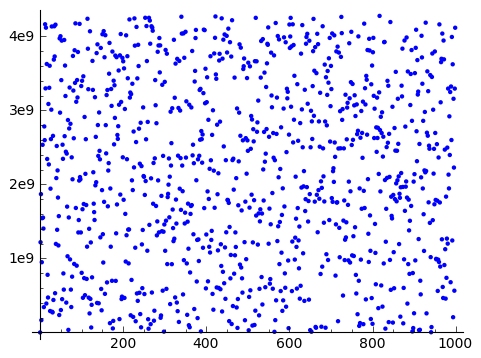
\includegraphics{sage0.png}
\caption{1000 liczb losowych wygenerowanych generatorem liniowym LCG}\end{figure}

Jak widać, program generuje liczby losowe z zakresu {[}0,m).


\paragraph{Rejestr przesuwający z liniowym sprzężeniem zwrotnym}
\label{ch5/chV011:rejestr-przesuwajacy-z-liniowym-sprzezeniem-zwrotnym}
TBA


\paragraph{Generator Wichmanna -- Hilla}
\label{ch5/chV011:generator-wichmanna-hilla}
TBA


\paragraph{Mersenne Twister}
\label{ch5/chV011:id3}
TBA

W dalszej części wykładu (a raczej ćwiczeń) będziemy bazować na domyślnym generowaniu liczb losowych w Sage.
Posłuży nam do tego wspominana już funkcja \code{random()} zwracająca liczbę pseudolosową o rozkładzie jednorodnym
na odcinku {[}0,1) (co często oznaczane jest poprzez $U(0,1)$).
\begin{gather}
\begin{split}U(0,1) = \left\{ \begin{array}{l l} 1 & \quad 0 \le x < 1\\ 0 & \quad \text{poza}\\ \end{array} \right.\end{split}\notag
\end{gather}
Aby uzyskać liczbę z przedziału {[}0,12.76)
wystarczy po prostu pomnożyć liczbę zwracną przez \code{random()} przez prawą granicę

\begin{Verbatim}[commandchars=\\\{\}]
\PYG{n}{random}\PYG{p}{(}\PYG{p}{)}\PYG{o}{*}\PYG{l+m+mf}{12.76}
\end{Verbatim}

a żeby uzyskać listę 123 liczb z przedziału {[}-13.3, 33.1) należy wykonać

\begin{Verbatim}[commandchars=\\\{\}]
\PYG{p}{[}\PYG{n}{random}\PYG{p}{(}\PYG{p}{)}\PYG{o}{*}\PYG{p}{(}\PYG{l+m+mf}{33.1}\PYG{o}{+}\PYG{l+m+mf}{13.3}\PYG{p}{)} \PYG{o}{\PYGZhy{}} \PYG{l+m+mf}{13.3} \PYG{k}{for} \PYG{n}{i} \PYG{o+ow}{in} \PYG{n+nb}{xrange}\PYG{p}{(}\PYG{l+m+mi}{123}\PYG{p}{)}\PYG{p}{]}
\end{Verbatim}

W ogólności do wygenerowania listy N liczb losowych z przedziału {[}A,B) należy użyć polecenia

\begin{Verbatim}[commandchars=\\\{\}]
\PYG{n}{N} \PYG{o}{=} \PYG{l+m+mi}{100}
\PYG{n}{A} \PYG{o}{=} \PYG{o}{\PYGZhy{}}\PYG{l+m+mi}{10}
\PYG{n}{B} \PYG{o}{=} \PYG{l+m+mi}{20}
\PYG{p}{[}\PYG{n}{random}\PYG{p}{(}\PYG{p}{)}\PYG{o}{*}\PYG{p}{(}\PYG{n}{B}\PYG{o}{\PYGZhy{}}\PYG{n}{A}\PYG{p}{)} \PYG{o}{+} \PYG{n}{A} \PYG{k}{for} \PYG{n}{i} \PYG{o+ow}{in} \PYG{n+nb}{xrange}\PYG{p}{(}\PYG{n}{N}\PYG{p}{)}\PYG{p}{]}
\end{Verbatim}
\begin{description}
\item[{Zadanie 2.2.2}] \leavevmode
Zmodyfikuj definicję \code{mylcg} tak, aby funkcja zwracała liczby losowe z przedziału {[}0,1).

\item[{Zadanie 2.2.3}] \leavevmode
LCG zdefiniowany tak jak powyżej produkuje stosunkowo dobre liczby losowe (prace naukowe
nad tym stosunkowo prostym generatorem trwają do dzisiaj, dowodzone są coraz to inne
okresy bazujące na wyborze różnych zestawów parametrów $a,c,m$). Naszym zadaniem
będzie natomiast zepsucie takiego generatora. Proszę znaleźć (numerycznie) 4 zestawy
parametrów definiujących LCG takich, aby okres generatora był krótki. Wykreśl w Sage
4 rysunki LCG(N) (dla powiedzmy N=1000) dla owych parametrów. Powinieneś zauważyć
regularność.

\end{description}


\subsection{Generowanie liczb losowych o zadanym rozkładzie}
\label{ch5/chV011:generowanie-liczb-losowych-o-zadanym-rozkladzie}
Jako, że już dysponujemy generatorem liczb losowych o rozkładzie jednostajnym na odcinku
$[0,1) - U(0,1)$ to możemy pokusić się o wygenerowanie liczb losowych o różnych innych rozkładach
prawdopodobieństwa. Znane jest kilka metod generowania takich liczb. Wszystkie przedstawione
tutaj będą opierały się na tym, że umiemy generować liczby z rozkładem U(0,1). Szczególną uwagę
poświęcimy generowaniu liczb z rozkładem N(0,1). Jest to standardowy zapis oznaczający rozkład
normalny (Gaussa) o średniej równej 0 i odchyleniu standardowym równym 1.
Zanim omówimy pierwszą metodę, wcześniej zdefiniujemy sobie pojęcie
\emph{histogramu}. Będzie nam on potrzebny do wizualizacji rozkładów (czy raczej ich gęstości) z wygenerowanych
liczb losowych.


\subsubsection{Histogram}
\label{ch5/chV011:histogram}
Wikipedia definiuje histogram jako jeden z graficznych sposobów przedstawiania rozkładu empirycznego cechy.
Konstruuje się go jako szereg prostokątów odpowiadających liczebności elementów wpadających do określonego
przedziału klasowego. Szerokości przedziałów klasowych mogą mieć stałe lub zmienne długości. W bardziej
matematycznym sensie histogram to funkcja zliczająca ilość obserwacji pasujących do oddzielnych przedziałów
klasowych. Jeżeli \emph{n} oznacza liczbę wszystkich obserwacji, a \emph{k} to liczba przedziałów, wtedy histogram
$m_i$ spełnia następujący warunek
\begin{gather}
\begin{split}n = \sum_{i=1}^k m_i\end{split}\notag
\end{gather}
Ideę histogramu najlepiej zrozumiec na przykładzie. Mamy następującą listę liczb

\begin{Verbatim}[commandchars=\\\{\}]
\PYG{n}{l} \PYG{o}{=} \PYG{p}{[}\PYG{l+m+mi}{1}\PYG{p}{,} \PYG{o}{\PYGZhy{}}\PYG{l+m+mi}{3}\PYG{p}{,} \PYG{o}{\PYGZhy{}}\PYG{l+m+mi}{5}\PYG{p}{,} \PYG{o}{\PYGZhy{}}\PYG{l+m+mi}{1}\PYG{p}{,} \PYG{o}{\PYGZhy{}}\PYG{l+m+mi}{3}\PYG{p}{,} \PYG{l+m+mi}{1}\PYG{p}{,} \PYG{l+m+mi}{5}\PYG{p}{,} \PYG{l+m+mi}{1}\PYG{p}{,} \PYG{l+m+mi}{3}\PYG{p}{,} \PYG{o}{\PYGZhy{}}\PYG{l+m+mi}{3}\PYG{p}{,} \PYG{l+m+mi}{4}\PYG{p}{,} \PYG{l+m+mi}{2}\PYG{p}{,} \PYG{l+m+mi}{4}\PYG{p}{,} \PYG{o}{\PYGZhy{}}\PYG{l+m+mi}{1}\PYG{p}{,} \PYG{l+m+mi}{4}\PYG{p}{,} \PYG{l+m+mi}{5}\PYG{p}{,} \PYG{o}{\PYGZhy{}}\PYG{l+m+mi}{2}\PYG{p}{,} \PYG{l+m+mi}{4}\PYG{p}{,} \PYG{l+m+mi}{3}\PYG{p}{,} \PYG{o}{\PYGZhy{}}\PYG{l+m+mi}{4}\PYG{p}{]}
\end{Verbatim}

Budując histogram na początku musimy ustalić szerokość przedziału. Zacznijmy od łatwiejszej wersji: niech
szerokość będzie stała. Najlepiej podzielić ową listę na przedziały zawierające liczby całkowite. W zasadzie
wystarczy zliczać ile jest poszczególnych liczb całkowitych w liście l. Zróbmy to. Widzimy, że mamy

\begin{tabulary}{\linewidth}{|L|L|L|L|L|L|L|L|L|L|L|}
\hline
\textbf{
-5
} & \textbf{
-4
} & \textbf{
-3
} & \textbf{
-2
} & \textbf{
-1
} & \textbf{
0
} & \textbf{
1
} & \textbf{
2
} & \textbf{
3
} & \textbf{
4
} & \textbf{
5
}\\\hline

1
 & 
1
 & 
3
 & 
1
 & 
2
 & 
0
 & 
3
 & 
1
 & 
2
 & 
4
 & 
2
\\\hline
\end{tabulary}


W zasadzie mamy już nasz histogram. Jeżeli posumujemy ilość elementów listy (\code{len(l)}), oraz obliczymy \emph{n}
zobaczymy, że dostaniemy tą samą liczbę (=20). Pozostaje narysować ów histogram. Na odciętej musimy odłożyć
przedziały klasowe a na rzędnej liczebności danego przedziału. Przyjęło się rysować histogram używając
słupków. Sage na chwilę obecną posiada kilka metod narysowania takiego histogramu. Jeżeli nie zależy nam na
poprawnym opisaniu odciętej (np: chcemy tylko zobaczyć kształt histogramu), wystarczy napisać

\begin{Verbatim}[commandchars=\\\{\}]
\PYG{n}{h} \PYG{o}{=} \PYG{p}{[}\PYG{n}{l}\PYG{o}{.}\PYG{n}{count}\PYG{p}{(}\PYG{n}{i}\PYG{p}{)} \PYG{k}{for} \PYG{n}{i} \PYG{o+ow}{in} \PYG{n+nb}{range}\PYG{p}{(}\PYG{o}{\PYGZhy{}}\PYG{l+m+mi}{5}\PYG{p}{,}\PYG{l+m+mi}{6}\PYG{p}{)}\PYG{p}{]}
\PYG{n}{bar\PYGZus{}chart}\PYG{p}{(}\PYG{n}{h}\PYG{p}{,} \PYG{n}{width}\PYG{o}{=}\PYG{l+m+mi}{1}\PYG{p}{,} \PYG{n}{color}\PYG{o}{=}\PYG{l+s}{\PYGZdq{}}\PYG{l+s}{orangered}\PYG{l+s}{\PYGZdq{}}\PYG{p}{)}\PYG{o}{.}\PYG{n}{show}\PYG{p}{(}\PYG{n}{axes\PYGZus{}labels}\PYG{o}{=}\PYG{p}{[}\PYG{l+s}{\PYGZsq{}}\PYG{l+s}{\PYGZdl{}i\PYGZdl{}}\PYG{l+s}{\PYGZsq{}}\PYG{p}{,}\PYG{l+s}{\PYGZsq{}}\PYG{l+s}{\PYGZdl{}}\PYG{l+s}{\PYGZbs{}}\PYG{l+s}{\PYGZsh{}\PYGZdl{}}\PYG{l+s}{\PYGZsq{}}\PYG{p}{]}\PYG{p}{,} \PYG{n}{title}\PYG{o}{=}\PYG{l+s}{\PYGZdq{}}\PYG{l+s}{histogram}\PYG{l+s}{\PYGZdq{}}\PYG{p}{)}
\end{Verbatim}

Co pozwoli nam wygenerować taki rysunek:
\begin{figure}[htbp]
\centering
\capstart

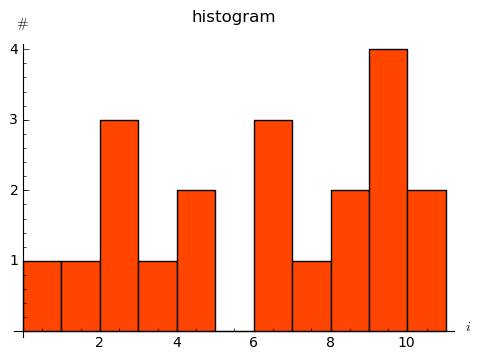
\includegraphics{bar_chart.png}
\caption{Prosty wykres liczebności, gdzie wykorzystaliśmy funkcję bar\_chart().}\end{figure}

Nie jest to prawdziwy histogram, bowiem odłożone na osi OY liczebności powinny odpowiadać rzeczywistym
wartościom (przedziałom). Możemy skorzystać z pakietu \code{Time Series} dostępnego w Sage. Wystarczą
prosta komenda aby uzyskać dostęp do wielu statystycznych funkcji typowych dla analizy szeregu czasowego.

\begin{Verbatim}[commandchars=\\\{\}]
\PYG{n}{v} \PYG{o}{=} \PYG{n}{finance}\PYG{o}{.}\PYG{n}{TimeSeries}\PYG{p}{(}\PYG{n}{l}\PYG{p}{)}
\end{Verbatim}

I teraz aby obliczyć histogram dla 10 równych przedziałów (od minimalnej do maksymalnej wartości występującej
w liście \code{l}), wystarczy napisać

\begin{Verbatim}[commandchars=\\\{\}]
\PYG{n}{v}\PYG{o}{.}\PYG{n}{histogram}\PYG{p}{(}\PYG{n}{bins}\PYG{o}{=}\PYG{l+m+mi}{11}\PYG{p}{)}
\end{Verbatim}

a aby narysować jego wykres

\begin{Verbatim}[commandchars=\\\{\}]
\PYG{n}{v}\PYG{o}{.}\PYG{n}{plot\PYGZus{}histogram}\PYG{p}{(}\PYG{n}{bins}\PYG{o}{=}\PYG{l+m+mi}{11}\PYG{p}{,} \PYG{n}{normalize}\PYG{o}{=}\PYG{l+m+mi}{0}\PYG{p}{,} \PYG{n}{color}\PYG{o}{=}\PYG{l+s}{\PYGZdq{}}\PYG{l+s}{orangered}\PYG{l+s}{\PYGZdq{}}\PYG{p}{,} \PYG{n}{axes\PYGZus{}labels}\PYG{o}{=}\PYG{p}{[}\PYG{l+s}{\PYGZsq{}}\PYG{l+s}{\PYGZdl{}i\PYGZdl{}}\PYG{l+s}{\PYGZsq{}}\PYG{p}{,}\PYG{l+s}{\PYGZsq{}}\PYG{l+s}{\PYGZdl{}}\PYG{l+s}{\PYGZbs{}}\PYG{l+s}{\PYGZsh{}\PYGZdl{}}\PYG{l+s}{\PYGZsq{}}\PYG{p}{]}\PYG{p}{)}
\end{Verbatim}
\begin{figure}[htbp]
\centering
\capstart

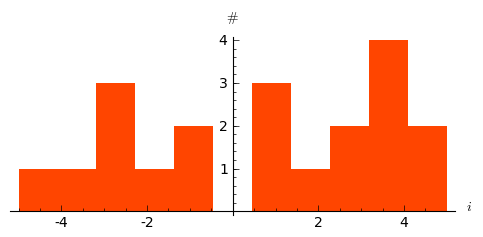
\includegraphics{histogram.png}
\caption{Histogram dla listy \code{l} uzyskany z wykorzystaniem pakietu \code{TimeSeries}}\end{figure}

Oczywiście całą procedurę można powtórzyć dla liczb zmiennoprzecinkowych (rzeczywistych, wymiernych). W tym
wypadku należałoby oczywiście policzyć ile posiadanych liczb wpada do zdefiniowanych ``pudełek''. Zobaczmy drugi
przykład, gdzie obliczymy i narysujemy w Sage histogram dla dziesięciu tysięcy liczb z U(0,1). Powinniśmy dostać
\begin{figure}[htbp]
\centering
\capstart

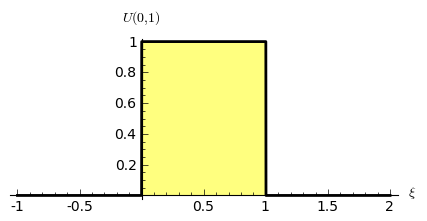
\includegraphics{u01.png}
\caption{Wykres rozkładu U(0,1)}\end{figure}
\begin{description}
\item[{Przykład 2}] \leavevmode
Wygenerujemy 10000 liczb losowych a następnie dla nich obliczymy i narysujemy histogram.

\begin{Verbatim}[commandchars=\\\{\}]
\PYG{n}{N} \PYG{o}{=} \PYG{l+m+mi}{10000}
\PYG{n}{u01} \PYG{o}{=} \PYG{p}{[}\PYG{n}{random}\PYG{p}{(}\PYG{p}{)} \PYG{k}{for} \PYG{n}{i} \PYG{o+ow}{in} \PYG{n+nb}{xrange}\PYG{p}{(}\PYG{n}{N}\PYG{p}{)}\PYG{p}{]}
\PYG{n}{fu01} \PYG{o}{=} \PYG{k}{lambda} \PYG{n}{x}\PYG{p}{:} \PYG{l+m+mi}{0} \PYG{k}{if} \PYG{n}{x} \PYG{o}{\PYGZlt{}} \PYG{l+m+mi}{0} \PYG{o+ow}{or} \PYG{n}{x} \PYG{o}{\PYGZgt{}} \PYG{l+m+mi}{1} \PYG{k}{else} \PYG{l+m+mi}{1}
\PYG{n}{v} \PYG{o}{=} \PYG{n}{finance}\PYG{o}{.}\PYG{n}{TimeSeries}\PYG{p}{(}\PYG{p}{[}\PYG{n}{random}\PYG{p}{(}\PYG{p}{)} \PYG{k}{for} \PYG{n}{i} \PYG{o+ow}{in} \PYG{n+nb}{xrange}\PYG{p}{(}\PYG{n}{N}\PYG{p}{)}\PYG{p}{]}\PYG{p}{)}
\PYG{n}{plot1} \PYG{o}{=} \PYG{n}{plot}\PYG{p}{(}\PYG{n}{fu01}\PYG{p}{,}\PYG{p}{(}\PYG{o}{\PYGZhy{}}\PYG{l+m+mi}{1}\PYG{p}{,}\PYG{l+m+mi}{2}\PYG{p}{)}\PYG{p}{,} \PYG{n}{thickness}\PYG{o}{=}\PYG{l+m+mi}{1}\PYG{p}{,} \PYG{n}{color}\PYG{o}{=}\PYG{l+s}{\PYGZdq{}}\PYG{l+s}{black}\PYG{l+s}{\PYGZdq{}}\PYG{p}{)}
\PYG{n}{plot2} \PYG{o}{=} \PYG{n}{v}\PYG{o}{.}\PYG{n}{plot\PYGZus{}histogram}\PYG{p}{(}\PYG{n}{bins}\PYG{o}{=}\PYG{l+m+mi}{10}\PYG{p}{,} \PYG{n}{color}\PYG{o}{=}\PYG{l+s}{\PYGZdq{}}\PYG{l+s}{orangered}\PYG{l+s}{\PYGZdq{}}\PYG{p}{)}
\PYG{p}{(}\PYG{n}{plot1} \PYG{o}{+} \PYG{n}{plot2}\PYG{p}{)}\PYG{o}{.}\PYG{n}{show}\PYG{p}{(}\PYG{n}{axes\PYGZus{}labels}\PYG{o}{=}\PYG{p}{[}\PYG{l+s}{r\PYGZsq{}}\PYG{l+s}{\PYGZdl{}}\PYG{l+s}{\PYGZbs{}}\PYG{l+s}{xi\PYGZdl{}}\PYG{l+s}{\PYGZsq{}}\PYG{p}{,}\PYG{l+s}{r\PYGZsq{}}\PYG{l+s}{\PYGZdl{}U(0,1)\PYGZdl{}}\PYG{l+s}{\PYGZsq{}}\PYG{p}{]}\PYG{p}{)}
\end{Verbatim}

\end{description}

Ostatnia linia wyrysuje nam obie funkcje na jednym wykresie. Zachęcamy czytelnika do poeksperymentowania z
powyższym kodem - można zmienić liczbę prób \emph{N} i łatwo zobaczyć jak histogram zaczyna oddalać się od
teoretycznego rozkładu dla małych N i jak zbliża się dla dużych. Można też zobaczyć jak ilość przedziałów
(parametr \code{bins}) wpływa na otrzymany histogram.
\begin{figure}[htbp]
\centering
\capstart

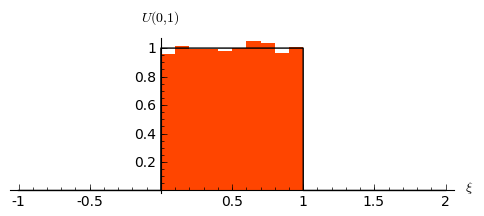
\includegraphics{u01_hist.png}
\caption{Wykres rozkładu U(0,1) + histogram miliona prób.}\end{figure}


\subsubsection{Metoda inwersyjna}
\label{ch5/chV011:metoda-inwersyjna}
Każdy rozkład prawdopodobieństwa może być jednoznacznie scharakteryzowany poprzez pewną funkcję
rzeczywistą zwaną \textbf{dystrybuantą}.
\begin{description}
\item[{Dystrybuanta}] \leavevmode
Niech $\mathbb{P}$ będzie rozkładem prawdopodobieństwa. Funkcję
$\mathbb{F}: \mathbb{R} \to \mathbb{R}$ daną wzorem
\begin{gather}
\begin{split}\mathbb{F}(\xi) = \mathbb{P}((-\infty, \xi))\end{split}\notag
\end{gather}
nazywamy dystrybuantą rozkładu $\mathbb{P}$.

\end{description}

W metodzie inwersyjnej żądany rozkład o dystrybuancie $\mathbb{F}$ uzyskuje się poprzez przekształcenie
zmiennej losowej o rozkładzie U(0,1) za pomocą funkcji odwrotnej do $\mathbb{F}$.
\begin{description}
\item[{Twierdzenie}] \leavevmode
Załóżmy, że dystrybuanta $\mathbb{F}$ jest ściśle rosnąca. Jeśli zmienna losowa \emph{u} ma
rozkład \emph{U(0,1)} to $\mathbb{F}^{-1}(u)$ ma dystrybuantę $\mathbb{F}$.

\item[{Dowód}] \leavevmode
TBA

\end{description}

Algorytm wykorzystujący powyższe twierdzenie jest bardzo prosty i wygląda następująco:
\begin{enumerate}
\item {} 
Generujemy liczbę $u \in U(0.1)$.

\item {} 
Przekształcamy \emph{u} stosując

$x = \mathbb{F}^{-1}(u)$

Wynikowa liczba losowa $x$ posiada żądany rozkład $\mathbb{P}$.

\end{enumerate}

Oczywiście skuteczność tej metody zależy bezpośrednio od tego czy możemy łatwo obliczyć $\mathbb{F}^{-1}$.
Jeżeli tak - jest to najprostsza znana metoda generowania liczb losowych z danym rozkładem. Do rozkładów,
do których można zastosować tą metodę należą wszystkie rozkłady, których dystrybuanta znana jest jawnie \emph{oraz}
można ją łatwo odwrócić. O takich rozkładach powiemy sobie niżej.


\paragraph{Rozkład wykładniczy}
\label{ch5/chV011:rozklad-wykladniczy}
Przejdźmy wreszcie do generowania liczb losowych z rozkładem innym niż \emph{U(0,1)}. Na początek weźmy jeden
z najbardziej powszechnych, czy popularnych rozkładów prawdopodobieństwa - \textbf{rozkład wykładniczy}. Gęstość
takiego rozkładu dana jest wzorem
\begin{gather}
\begin{split}f(\xi) = \lambda e^{-\lambda \xi}\end{split}\notag
\end{gather}
Jak łatwo policzyć, dystrybuanta \emph{F(x)} wynosi
\begin{gather}
\begin{split}F(x) = \int_{-\infty}^x f(\xi) d\xi = -e^{-\lambda \xi}\Big|_{-\infty}^x = -e^{-\lambda x} + 1,\end{split}\notag\\\begin{split}\end{split}\notag
\end{gather}
a jej odwrotność
\begin{gather}
\begin{split}F^{-1}(u) = -\frac{1}{\lambda} \ln (1-u).\end{split}\notag
\end{gather}
Spróbujmy wygenerować 5000 liczb o rozkładzie wykładniczym. Następnie obliczymy sobie histogram, unormujemy
go i porównamy z teoretycznym rozkładem dla kilku wartości $\lambda = 0.5, 1, 1.5$.

\begin{Verbatim}[commandchars=\\\{\}]
\PYG{n}{f}\PYG{p}{(}\PYG{n}{xi}\PYG{p}{,} \PYG{n}{a}\PYG{p}{)} \PYG{o}{=} \PYG{n}{a} \PYG{o}{*} \PYG{n}{exp}\PYG{p}{(}\PYG{o}{\PYGZhy{}}\PYG{n}{a} \PYG{o}{*} \PYG{n}{xi}\PYG{p}{)}
\PYG{n}{F}\PYG{p}{(}\PYG{n}{u}\PYG{p}{,} \PYG{n}{a}\PYG{p}{)} \PYG{o}{=} \PYG{o}{\PYGZhy{}}\PYG{n}{log}\PYG{p}{(}\PYG{l+m+mi}{1}\PYG{o}{\PYGZhy{}}\PYG{n}{u}\PYG{p}{)}\PYG{o}{/}\PYG{n}{a}
\PYG{n}{N} \PYG{o}{=} \PYG{l+m+mi}{5000}
\PYG{n}{kolor} \PYG{o}{=} \PYG{p}{[}\PYG{l+s}{\PYGZdq{}}\PYG{l+s}{red}\PYG{l+s}{\PYGZdq{}}\PYG{p}{,} \PYG{l+s}{\PYGZdq{}}\PYG{l+s}{green}\PYG{l+s}{\PYGZdq{}}\PYG{p}{,} \PYG{l+s}{\PYGZdq{}}\PYG{l+s}{blue}\PYG{l+s}{\PYGZdq{}}\PYG{p}{]}
\PYG{n}{parlist} \PYG{o}{=} \PYG{p}{[}\PYG{l+m+mf}{1.5}\PYG{p}{,} \PYG{l+m+mi}{1}\PYG{p}{,} \PYG{l+m+mf}{0.5}\PYG{p}{]}
\PYG{n}{p} \PYG{o}{=} \PYG{p}{[}\PYG{p}{]}
\PYG{k}{for} \PYG{n}{par} \PYG{o+ow}{in} \PYG{n}{parlist}\PYG{p}{:}
  \PYG{n}{lista} \PYG{o}{=} \PYG{p}{[}\PYG{n}{F}\PYG{p}{(}\PYG{n}{random}\PYG{p}{(}\PYG{p}{)}\PYG{p}{,} \PYG{n}{par}\PYG{p}{)} \PYG{k}{for} \PYG{n}{i} \PYG{o+ow}{in} \PYG{n+nb}{xrange}\PYG{p}{(}\PYG{n}{N}\PYG{p}{)}\PYG{p}{]}
  \PYG{n}{v} \PYG{o}{=} \PYG{n}{finance}\PYG{o}{.}\PYG{n}{TimeSeries}\PYG{p}{(}\PYG{n}{lista}\PYG{p}{)}
  \PYG{n}{P} \PYG{o}{=} \PYG{n}{v}\PYG{o}{.}\PYG{n}{plot\PYGZus{}histogram}\PYG{p}{(}\PYG{n}{bins}\PYG{o}{=}\PYG{l+m+mi}{100}\PYG{p}{,} \PYG{n}{color}\PYG{o}{=}\PYG{n}{kolor}\PYG{p}{[}\PYG{n}{parlist}\PYG{o}{.}\PYG{n}{index}\PYG{p}{(}\PYG{n}{par}\PYG{p}{)}\PYG{p}{]}\PYG{p}{,} \PYG{n}{alpha}\PYG{o}{=}\PYG{l+m+mf}{0.5}\PYG{p}{)}
  \PYG{n}{P}\PYG{o}{.}\PYG{n}{set\PYGZus{}aspect\PYGZus{}ratio}\PYG{p}{(}\PYG{l+s}{\PYGZdq{}}\PYG{l+s}{automatic}\PYG{l+s}{\PYGZdq{}}\PYG{p}{)}
  \PYG{n}{p}\PYG{o}{.}\PYG{n}{append}\PYG{p}{(}\PYG{n}{P}\PYG{p}{)}
  \PYG{n}{p}\PYG{o}{.}\PYG{n}{append}\PYG{p}{(}\PYG{n}{plot}\PYG{p}{(}\PYG{n}{f}\PYG{p}{(}\PYG{n}{xi}\PYG{p}{,}\PYG{n}{par}\PYG{p}{)}\PYG{p}{,} \PYG{l+m+mi}{0}\PYG{p}{,} \PYG{n+nb}{max}\PYG{p}{(}\PYG{n}{lista}\PYG{p}{)}\PYG{p}{,} \PYG{n}{thickness}\PYG{o}{=}\PYG{l+m+mi}{2}\PYG{p}{,} \PYG{n}{color}\PYG{o}{=}\PYG{n}{kolor}\PYG{p}{[}\PYG{n}{parlist}\PYG{o}{.}\PYG{n}{index}\PYG{p}{(}\PYG{n}{par}\PYG{p}{)}\PYG{p}{]}\PYG{p}{,}
  \PYG{n}{legend\PYGZus{}label}\PYG{o}{=}\PYG{l+s}{r\PYGZsq{}}\PYG{l+s}{\PYGZdl{}}\PYG{l+s}{\PYGZbs{}}\PYG{l+s}{lambda = }\PYG{l+s+si}{\PYGZpc{}.1f}\PYG{l+s}{\PYGZdl{}}\PYG{l+s}{\PYGZsq{}}\PYG{o}{\PYGZpc{}}\PYG{n}{par}\PYG{p}{)}\PYG{p}{)}
\PYG{n+nb}{sum}\PYG{p}{(}\PYG{n}{p}\PYG{p}{)}\PYG{o}{.}\PYG{n}{show}\PYG{p}{(}\PYG{n}{xmin}\PYG{o}{=}\PYG{l+m+mi}{0}\PYG{p}{,} \PYG{n}{xmax}\PYG{o}{=}\PYG{l+m+mi}{5}\PYG{p}{,} \PYG{n}{figsize}\PYG{o}{=}\PYG{l+m+mi}{5}\PYG{p}{,} \PYG{n}{axes\PYGZus{}labels}\PYG{o}{=}\PYG{p}{[}\PYG{l+s}{r\PYGZsq{}}\PYG{l+s}{\PYGZdl{}}\PYG{l+s}{\PYGZbs{}}\PYG{l+s}{xi\PYGZdl{}}\PYG{l+s}{\PYGZsq{}}\PYG{p}{,}\PYG{l+s}{r\PYGZsq{}}\PYG{l+s}{\PYGZdl{}}\PYG{l+s}{\PYGZbs{}}\PYG{l+s}{lambda e\PYGZca{}\PYGZob{}\PYGZhy{}}\PYG{l+s}{\PYGZbs{}}\PYG{l+s}{lambda }\PYG{l+s}{\PYGZbs{}}\PYG{l+s}{xi\PYGZcb{}\PYGZdl{}}\PYG{l+s}{\PYGZsq{}}\PYG{p}{]}\PYG{p}{,} \PYG{n}{fontsize}\PYG{o}{=}\PYG{l+m+mi}{12}\PYG{p}{)}
\end{Verbatim}

Jak widać na rysunku liczby losowe przekształcone metodą inwersji w oparciu o odwrotność dystrybuanty, dość dobrze
odwzorowują rozkład wykładniczy. Lepszy wynik można oczywiście uzyskać zwiększając parametry \code{N} oraz \code{bins}.
\begin{figure}[htbp]
\centering
\capstart

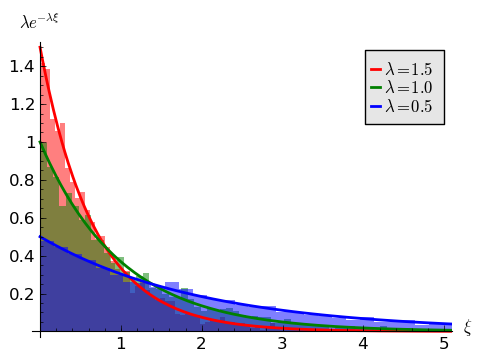
\includegraphics{r_exp_hist.png}
\caption{Wykres gęstości rozkładu wykładniczego oraz histogram z 5000 prób liczb losowych dla trzech wartości parametru
$\lambda$.}\end{figure}

Alternatywnie można wykorzystać przekształcenie bazujące na spostrzeżeniu, że liczby $1-u$ oraz
$u (u \in U(0,1)$ posiadają ten sam rozkład \emph{U(0,1)}.


\paragraph{Rozkład Cauchy'ego}
\label{ch5/chV011:rozklad-cauchy-ego}
Rozkład ten dany jest wzorem
\begin{gather}
\begin{split}f(\xi) = \frac{\sigma}{\pi (\xi^2 + \sigma^2)}\end{split}\notag
\end{gather}
Odwrotność dystrybuanty powyższego rozkładu wynosi
\begin{gather}
\begin{split}F^{-1}(u) = \sigma \tan \Big[\pi \Big(u - \frac{1}{2} \Big)\Big].\end{split}\notag\\\begin{split}\end{split}\notag
\end{gather}
Stosując proste i bardzo naturalne przekształcenie oryginalnej zmiennej $v = 1/2 - u$
dostajemy nieco prostsze wyrażenie
\begin{gather}
\begin{split}F^{-1}(v) = \sigma \tan (\pi v).\end{split}\notag
\end{gather}
Stosując podobne metody jak w poprzednim rozdziale możemy sprawdzić, czy powyższe przekształcenie
generuje liczby z odpowiednim rozkładem.
\begin{figure}[htbp]
\centering
\capstart

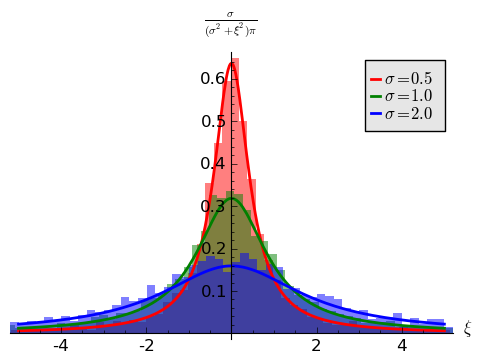
\includegraphics{r_cauchy_hist.png}
\caption{Wykres gęstości rozkładu Cauchy'ego oraz histogram z 5000 prób liczb losowych dla trzech wartości parametru
$\sigma = 0.5, 1, 2$.}\end{figure}


\paragraph{Rozkład logistyczny}
\label{ch5/chV011:rozklad-logistyczny}
Rozkład ten dany jest wzorem
\begin{gather}
\begin{split}f(\xi) = \frac{1}{2 + e^{\xi} + e^{-\xi}}\end{split}\notag
\end{gather}
Odwrotność dystrybuanty powyższego rozkładu wynosi
\begin{gather}
\begin{split}F^{-1}(u) = \ln\frac{u}{1-u}.\end{split}\notag\\\begin{split}\end{split}\notag
\end{gather}
Stosując podobne metody jak w poprzednim rozdziale możemy sprawdzić, czy powyższe przekształcenie
generuje liczby z odpowiednim rozkładem.
\begin{figure}[htbp]
\centering
\capstart

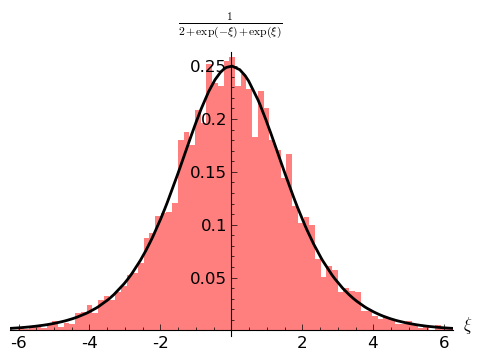
\includegraphics{r_logist_hist.png}
\caption{Wykres gęstości rozkładu logistycznego oraz histogram z 200000 prób liczb losowych.}\end{figure}
\begin{description}
\item[{Zadanie 2.3.1}] \leavevmode
Wygeneruj 200000 liczb losowych z rozkładem Pareto. Narysuj ich unormowany histogram oraz funkcję gęstości.
Porównaj obie funkcje zmieniając wszystkie parametry rozkładu.

\item[{Zadanie 2.3.2.}] \leavevmode
Wygeneruj 1000 liczb losowych z rozkładem trójkątnym. Narysuj ich unormowany histogram oraz funkcję gęstości.
Porównaj obie funkcje zmieniając wszystkie parametry rozkładu.

\end{description}


\bigskip\hrule{}\bigskip



\bigskip\hrule{}\bigskip



\section{Równania różniczkowe zwyczajne}
\label{ch5/chV012:python}\label{ch5/chV012::doc}\label{ch5/chV012:rownania-rozniczkowe-zwyczajne}

\subsection{Metoda Eulera}
\label{ch5/chV012:metoda-eulera}
Jest to bodaj najprostszy sposób na numeryczne rozwiązywanie równań różniczkowych
zwyczajnych. Technicznie to metoda pierwszego rzędu. Bazuje na prostej interpretacji
definicji pochodnej. Rozpatrujemy równanie postaci
\begin{gather}
\begin{split}\frac{dy}{ds} = y' = f(y,s),\end{split}\notag
\end{gather}
z zadanymi warunkami początkowymi $(sx(0), y(0)) = (x_0, y_0)$. Stosując przekształcenie
\begin{gather}
\begin{split}\frac{dy}{ds} = \lim_{\Delta s \to 0}\frac{\Delta y}{\Delta s}\end{split}\notag
\end{gather}
Na chwilę zapomnijmy o tej granicy. Mamy
\begin{gather}
\begin{split}\frac{\Delta y}{\Delta s} = \frac{y(s+\Delta s) - y(s)}{\Delta s}\end{split}\notag
\end{gather}
stawiając krok ``czasowy'' $\Delta x = h$ (jak to zwyczajowo w symulacjach komputerowych)
dostajemy
\begin{gather}
\begin{split}\frac{y(s + h) - y(s)}{h} \simeq f(y,s),\end{split}\notag\\\begin{split}y(s+h) \simeq y(s) + f(y,s) h.\end{split}\notag
\end{gather}
Oczywiście pełna równość zachodzi tylko w granicy $h \to 0$. Na potrzeby numeryczne jednak
nie musimy się tym przejmować. Należy mieć tylko świadomość, że zmniejszanie kroku czasowego
zbliża nas do wyniku dokładnego (zazwyczaj). Jako, że w iteracjach ``czasowych'' wykorzystujemy
stały krok $h$, więc w danej, powiedzmy \emph{i}-tej iteracji czas rzeczywisty zastąpiony zostanie
poprzez $s_i = i \cdot h$, możemy równie dobrze wprowadzić indeksowanie nie po czasie \emph{s} ale
po zmiennej iteracyjnej \emph{i}
\begin{gather}
\begin{split}y (s = ih) = y(s_i) = y_i, \quad s_i = i h,\end{split}\notag\\\begin{split}y (i h + h) = y(h(i+1)) = y(ih) + f(y(ih), ih) h,\end{split}\notag\\\begin{split}y_{i+1} = y_i + f(y_i,s_i) h.\end{split}\notag
\end{gather}
Dostając tzw. schemat Eulera. Innymi metodami wyprowadzenia tego prostego schematu będzie użycie
rozwinięcia Tylora lub wycałkowanie równania różniczowego od $s_0$ do :math{}`s\_0 + h{}`
za pomocą metody prostokątów (uzywając tylko jednego prostokąta na całym przedziale całkowania).
\begin{description}
\item[{Zadanie D1.1}] \leavevmode
Uzyskaj schemat Eulera z rozwinięcia Tylora.

\item[{Zadanie D1.2}] \leavevmode
Uzyskaj schemat Eulera całkując równanie różniczkowe.

\end{description}

Dokładność metody Eulera mocno zależy od wyboru kroku całkowania \emph{h}. Musimy też na początku zadać
warunki startowe (początkowe) iteracji, zupełnie jak podczas rozwiązywania równań metodami analitycznymi.
Dla przykładu obliczmy numerycznie ruch przetłumionego sprężyny o współczynniku sprężystości \emph{k}.
\begin{gather}
\begin{split}\dot{x}(t) = -k x(t).\end{split}\notag
\end{gather}
Rozwiązaniem jest zanik eksponencjalny $x(t) = x_0 \exp (-k t)$. Wybierzemy sobie warunek początkowy
$x_0 = 1$ i współczynnik sprężystości $k=0.1$. Policzmy \emph{N} iteracji i narysujmy wykres. Na
początku napiszemy dyskretną wersję równania ruchu
\begin{gather}
\begin{split}x_{i+1} = x_{i} - k x_i h = x_i (1 - kh).\end{split}\notag
\end{gather}
Teraz kod Sage

\begin{Verbatim}[commandchars=\\\{\}]
\PYG{c}{\PYGZsh{} liczba iteracji rownania}
\PYG{n}{N} \PYG{o}{=} \PYG{l+m+mi}{300}
\PYG{c}{\PYGZsh{} czas poczatkowy}
\PYG{n}{t} \PYG{o}{=} \PYG{l+m+mi}{0}
\PYG{c}{\PYGZsh{} skok czasowy}
\PYG{n}{h} \PYG{o}{=} \PYG{l+m+mf}{0.01}
\PYG{c}{\PYGZsh{} parametr rownania (sprezystosc)}
\PYG{n}{k} \PYG{o}{=} \PYG{l+m+mi}{1}
\PYG{c}{\PYGZsh{} wartosc poczatkowa x(t=0)}
\PYG{n}{x\PYGZus{}0} \PYG{o}{=} \PYG{l+m+mi}{1}
\PYG{c}{\PYGZsh{}inicializacja listy poprzez wartosc poczatkowa}
\PYG{n}{lista\PYGZus{}x} \PYG{o}{=} \PYG{p}{[}\PYG{n}{x\PYGZus{}0}\PYG{p}{]}
\PYG{k}{for} \PYG{n}{i} \PYG{o+ow}{in} \PYG{n+nb}{xrange}\PYG{p}{(}\PYG{n}{N}\PYG{p}{)}\PYG{p}{:}
  \PYG{n}{lista\PYGZus{}x}\PYG{o}{.}\PYG{n}{append}\PYG{p}{(}\PYG{n}{lista\PYGZus{}x}\PYG{p}{[}\PYG{n}{i}\PYG{p}{]} \PYG{o}{*} \PYG{p}{(}\PYG{l+m+mi}{1} \PYG{o}{\PYGZhy{}} \PYG{n}{k}\PYG{o}{*}\PYG{n}{h}\PYG{p}{)}\PYG{p}{)}
\end{Verbatim}

wynik (rozwiąznanie numeryczne równania) trzymany jest w liście \code{lista\_x}. Wyrysujmy ją standardowo, razem
z wynikiem analitycznym.
\begin{figure}[htbp]
\centering
\capstart

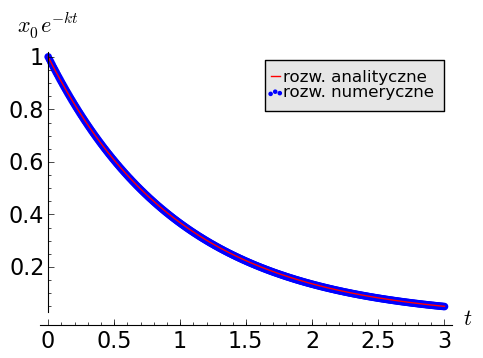
\includegraphics{euler001.png}
\caption{Rozwiązanie analityczne i numeryczne równania $\dot{x} = -kx$.}\end{figure}

Pomimo użycia prostej metody (pierwszego rzędu), wykresy wyglądają identycznie. No, ale czy na pewno jest tak pięknie?
Poprawność metody możemy łatwo zbadać obliczając błędy względny ($E_w$) i bezwzględny ($E_b$).
\begin{gather}
\begin{split}E_b = \bar{y} - y,\end{split}\notag\\\begin{split}E_w = \frac{\bar{y} - y}{\bar{y}} = \frac{E_b}{\bar{y}}.\end{split}\notag
\end{gather}
gdzie $y$ to wielkość obliczona algorytmem a $\bar{y}$ to dokładna wielkość analityczna. Dla jasności -
nie interesują nas w tym przypadku znaki błędów a jedynie ich wartość bezwzględna (tu proszę zwrócić
uwage na nomenklaturę, żeby nie pomylić wartości bezwzględnej z błędem bezwzględnym). Dlatego najczęściej
oblicza się nie $E_w$ a $|E_w|$. Wymaga to drobnej korekty powyższego kodu

\begin{Verbatim}[commandchars=\\\{\}]
\PYG{n}{N}\PYG{p}{,} \PYG{n}{t}\PYG{p}{,} \PYG{n}{h}\PYG{p}{,} \PYG{n}{k}\PYG{p}{,} \PYG{n}{x\PYGZus{}0} \PYG{o}{=} \PYG{l+m+mi}{1000}\PYG{p}{,} \PYG{l+m+mi}{0}\PYG{p}{,} \PYG{l+m+mf}{0.01}\PYG{p}{,} \PYG{l+m+mi}{1}\PYG{p}{,} \PYG{l+m+mi}{1}
\PYG{n}{g}\PYG{p}{(}\PYG{n}{s}\PYG{p}{)} \PYG{o}{=} \PYG{n}{x\PYGZus{}0}\PYG{o}{*}\PYG{n}{exp}\PYG{p}{(}\PYG{o}{\PYGZhy{}}\PYG{n}{k}\PYG{o}{*}\PYG{n}{s}\PYG{p}{)}
\PYG{n}{lista\PYGZus{}x} \PYG{o}{=} \PYG{p}{[}\PYG{n}{x\PYGZus{}0}\PYG{p}{]}
\PYG{n}{Eb} \PYG{o}{=} \PYG{p}{[}\PYG{n}{g}\PYG{p}{(}\PYG{l+m+mi}{0}\PYG{p}{)} \PYG{o}{\PYGZhy{}} \PYG{n}{x\PYGZus{}0}\PYG{p}{]}
\PYG{n}{Ew} \PYG{o}{=} \PYG{p}{[}\PYG{n}{Ew}\PYG{p}{[}\PYG{l+m+mi}{0}\PYG{p}{]}\PYG{o}{/}\PYG{n}{g}\PYG{p}{(}\PYG{l+m+mi}{0}\PYG{p}{)}\PYG{p}{]}
\PYG{k}{for} \PYG{n}{i} \PYG{o+ow}{in} \PYG{n+nb}{xrange}\PYG{p}{(}\PYG{l+m+mi}{1}\PYG{p}{,}\PYG{n}{N}\PYG{p}{)}\PYG{p}{:}
  \PYG{n}{lista\PYGZus{}x}\PYG{o}{.}\PYG{n}{append}\PYG{p}{(}\PYG{n}{lista\PYGZus{}x}\PYG{p}{[}\PYG{n}{i}\PYG{o}{\PYGZhy{}}\PYG{l+m+mi}{1}\PYG{p}{]} \PYG{o}{*} \PYG{p}{(}\PYG{l+m+mi}{1} \PYG{o}{\PYGZhy{}} \PYG{n}{k}\PYG{o}{*}\PYG{n}{h}\PYG{p}{)}\PYG{p}{)}
  \PYG{n}{Eb}\PYG{o}{.}\PYG{n}{append}\PYG{p}{(}\PYG{n+nb}{abs}\PYG{p}{(}\PYG{n}{g}\PYG{p}{(}\PYG{n}{i}\PYG{o}{*}\PYG{n}{h}\PYG{p}{)} \PYG{o}{\PYGZhy{}} \PYG{n}{lista\PYGZus{}x}\PYG{p}{[}\PYG{n}{i}\PYG{p}{]}\PYG{p}{)}\PYG{p}{)}
  \PYG{n}{Ew}\PYG{o}{.}\PYG{n}{append}\PYG{p}{(}\PYG{n}{Eb}\PYG{p}{[}\PYG{n}{i}\PYG{p}{]}\PYG{o}{/}\PYG{n}{g}\PYG{p}{(}\PYG{n}{i}\PYG{o}{*}\PYG{n}{h}\PYG{p}{)}\PYG{p}{)}
\PYG{n}{list\PYGZus{}plot}\PYG{p}{(}\PYG{n+nb}{zip}\PYG{p}{(}\PYG{p}{[}\PYG{n}{i}\PYG{o}{*}\PYG{n}{h} \PYG{k}{for} \PYG{n}{i} \PYG{o+ow}{in} \PYG{n+nb}{xrange}\PYG{p}{(}\PYG{n}{N}\PYG{o}{+}\PYG{l+m+mi}{1}\PYG{p}{)}\PYG{p}{]}\PYG{p}{,}\PYG{n}{Eb}\PYG{p}{)}\PYG{p}{)}\PYG{o}{.}\PYG{n}{show}\PYG{p}{(}\PYG{p}{)}
\PYG{n}{list\PYGZus{}plot}\PYG{p}{(}\PYG{n+nb}{zip}\PYG{p}{(}\PYG{p}{[}\PYG{n}{i}\PYG{o}{*}\PYG{n}{h} \PYG{k}{for} \PYG{n}{i} \PYG{o+ow}{in} \PYG{n+nb}{xrange}\PYG{p}{(}\PYG{n}{N}\PYG{o}{+}\PYG{l+m+mi}{1}\PYG{p}{)}\PYG{p}{]}\PYG{p}{,}\PYG{n}{Ew}\PYG{p}{)}\PYG{p}{)}\PYG{o}{.}\PYG{n}{show}\PYG{p}{(}\PYG{p}{)}
\end{Verbatim}

Spójrzmy. Na pierwszym wykresie odłożony mamy błąd bezwzględny. Widzimy, że dla krótkich czasów odbiega on od wartości
analitycznej by dla większych czasów zmaleć do zera. Mogą być tego 2 powody: (i) różnica pomiędzy obiema wartościami
maleje zo zera lub (ii) obie wartości maleją do zera, więc ich różnica też. Jako, że funkcja jest eksponencjalna,
dużo bardziej prawdopodobny jest ten drugi scenariusz. Aby zobaczyć, czy błąd rośnie z ilością iteracji
(w czasie) wykreślimy błąd względny. Mówi on nam o stosunku błedu bezwzględnego do wartości analitycznej (rysunek
po prawej). Tu jak widać rośnie on wraz z czasem, z czego możemy wywnioskować, że wraz z ilością iteracji
coraz mniej dokładnie obliczamy wartość \emph{y}.
\begin{figure}[htbp]
\centering
\capstart

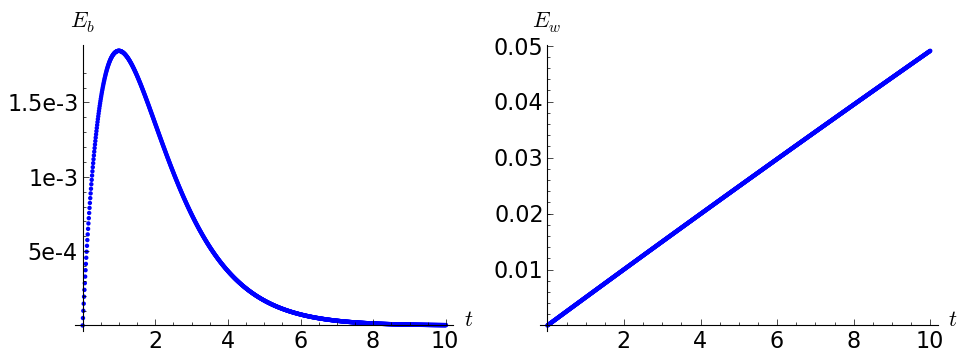
\includegraphics{euler_err.png}
\caption{Błąd bezwzględny (po lewej) i błąd względny (po prawej).}\end{figure}

Najprosztszą metodą poprawienia jakości rozwiązań jest zmniejszenie kroku całkowania. Zależności pozostaną podobne,
zmniejszy się jednak wartośc błędów w danej chwli czasowej.
\begin{figure}[htbp]
\centering
\capstart

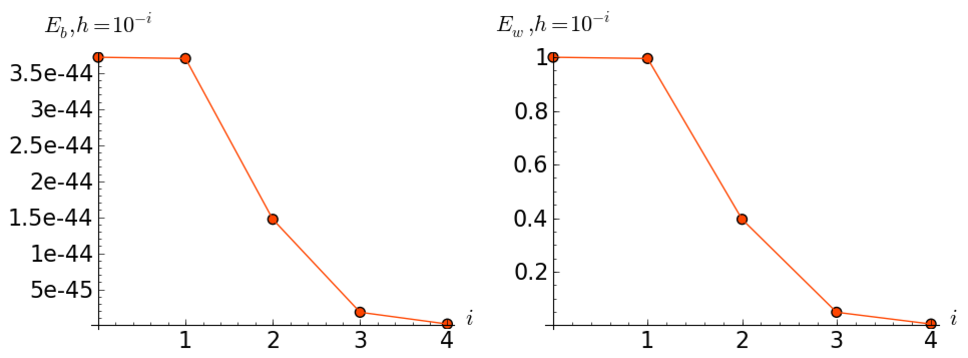
\includegraphics{euler_ebw_h.png}
\caption{Błąd bezwzględny (po lewej) i błąd względny (po prawej) po czasie $t=10$ dla różnych kroków czasowych
$h = 1, 0.1, 0.01, 0.001, 0.0001$.}\end{figure}

W tabeli zawarto wartości błędów bezwzględnego i względnego dla różnych wielkości kroku czasowego
symulacji, po osiągnięciu czasu końcowego $T_E = 10$. Widać, że pomimo, że za każdym zmniejszeniem
kroku zwiększała się ilość kroków czasowych, dokładność obliczeń rosła - malał zarówno błąd bezwzględny
jak i względny.

\begin{tabulary}{\linewidth}{|L|L|L|L|}
\hline

\emph{h}
 & 
\emph{N}
 & 
$E_b$
 & 
$E_w$
\\\hline

1
 & 
100
 & 
$3.72 10^{-44}$
 & 
1
\\\hline

0.1
 & 
1 000
 & 
$3.70 10^{-44}$
 & 
0.995
\\\hline

0.01
 & 
10 000
 & 
$1.47 10^{-44}$
 & 
0.396
\\\hline

0.001
 & 
100 000
 & 
$1.82 10^{-45}$
 & 
0.0488
\\\hline

0.0001
 & 
1 000 000
 & 
$1.86 10^{-46}$
 & 
0.0499
\\\hline
\end{tabulary}


Przejdźmy teraz do rozwiązania równania różniczkowego wyższego stopnia. Znów posłużymy się przykładem
oscylatora harmonicznego. Tym razem rozwiążemy równanie Newtona dla punktowej cząstki o masie \emph{m}
w potencjale $U(x) = -k x^2 / 2$. Pominiemy siły tarcia. Również w spokoju zostawimy wymuszenie.
\begin{gather}
\begin{split}m \ddot{x}(t) = -kx(t).\end{split}\notag
\end{gather}
Równanie to posiada znane
\href{http://ribes.if.uj.edu.pl/homepage/weblog/Oscylator\_harmoniczny\_rozwiazanie/Oscylator\_harmoniczny\_rozwiazanie.pdf}{analityczne rozwiązanie}.
Oznaczając $\omega_0^2 = k/m$ dostajemy
\begin{gather}
\begin{split}x(t) = A \sin(\omega_0 t) + B \cos(\omega_0 t).\end{split}\notag
\end{gather}
Stałe \emph{A, B} (amplitudy) zależne są od wyboru warunków początkowych. Spróbujmy numerycznie
rozwiązać równanie ruchu tak, aby pokazać zgodność z rozwiązaniem. Aby napisać schemat Eulera dla równania
drugiego stopnia najpierw trzeba przepisać równanie do układu równań na $x$ i $v = \dot{x}$.
\begin{gather}
\begin{split}\dot{x}(t) = v(t),\end{split}\notag\\\begin{split}\dot{v}(t) = -\frac{k}{m} x(t) = - \omega_0^2 x(t).\end{split}\notag
\end{gather}
Teraz wystarczy zdyskretyzować te równania, tak samo jak robiliśmy to z równaniem pierwszego rzędu.
\begin{gather}
\begin{split}x_{i+1} = x_i + v_i h,\end{split}\notag\\\begin{split}v_{i+1} = v_i - \omega^2_0 x_i h.\end{split}\notag
\end{gather}
Po ustaleniu warunków początkowych $x(0) = x_0$ oraz $v(0) = v_0$ możemy rozpocząć normalną
procedurę symulacji - wybieramy krok czasowy \emph{h}, ustalamy parametry równania i do dzieła.

\begin{Verbatim}[commandchars=\\\{\}]
\PYG{n}{h} \PYG{o}{=} \PYG{l+m+mf}{0.01} \PYG{c}{\PYGZsh{} skok}
\PYG{n}{N} \PYG{o}{=} \PYG{l+m+mi}{100} \PYG{c}{\PYGZsh{} liczba krokow}

\PYG{n}{x0} \PYG{o}{=} \PYG{l+m+mi}{1}
\PYG{n}{v0} \PYG{o}{=} \PYG{l+m+mi}{0}
\PYG{n}{omega0} \PYG{o}{=} \PYG{l+m+mi}{1}

\PYG{n}{lista\PYGZus{}x} \PYG{o}{=} \PYG{p}{[}\PYG{n}{x0}\PYG{p}{]}
\PYG{n}{lista\PYGZus{}v} \PYG{o}{=} \PYG{p}{[}\PYG{n}{v0}\PYG{p}{]}
\PYG{n}{lista\PYGZus{}t} \PYG{o}{=} \PYG{p}{[}\PYG{l+m+mi}{0}\PYG{p}{]}
\PYG{k}{for} \PYG{n}{i} \PYG{o+ow}{in} \PYG{n+nb}{xrange}\PYG{p}{(}\PYG{n}{N}\PYG{p}{)}\PYG{p}{:}
  \PYG{n}{lista\PYGZus{}x}\PYG{o}{.}\PYG{n}{append}\PYG{p}{(}\PYG{n}{lista\PYGZus{}x}\PYG{p}{[}\PYG{n}{i}\PYG{p}{]} \PYG{o}{+} \PYG{n}{lista\PYGZus{}v}\PYG{p}{[}\PYG{n}{i}\PYG{p}{]} \PYG{o}{*} \PYG{n}{h}\PYG{p}{)}
  \PYG{n}{lista\PYGZus{}v}\PYG{o}{.}\PYG{n}{append}\PYG{p}{(}\PYG{n}{lista\PYGZus{}v}\PYG{p}{[}\PYG{n}{i}\PYG{p}{]} \PYG{o}{\PYGZhy{}} \PYG{n}{omega0}\PYG{o}{\PYGZca{}}\PYG{l+m+mi}{2} \PYG{o}{*} \PYG{n}{lista\PYGZus{}x}\PYG{p}{[}\PYG{n}{i}\PYG{p}{]} \PYG{o}{*} \PYG{n}{h}\PYG{p}{)}
  \PYG{n}{lista\PYGZus{}t}\PYG{o}{.}\PYG{n}{append}\PYG{p}{(}\PYG{n}{lista\PYGZus{}t}\PYG{p}{[}\PYG{n}{i}\PYG{p}{]} \PYG{o}{+} \PYG{n}{h}\PYG{p}{)}
\end{Verbatim}

Wykorzystamy też Sage do obliczenia rozwiązania analitycznego dla naszego zagadnienia.

\begin{Verbatim}[commandchars=\\\{\}]
\PYG{n}{var}\PYG{p}{(}\PYG{l+s}{\PYGZsq{}}\PYG{l+s}{t x omega x\PYGZus{}0 v\PYGZus{}0}\PYG{l+s}{\PYGZsq{}}\PYG{p}{)}
\PYG{n}{x} \PYG{o}{=} \PYG{n}{function}\PYG{p}{(}\PYG{l+s}{\PYGZsq{}}\PYG{l+s}{x}\PYG{l+s}{\PYGZsq{}}\PYG{p}{,} \PYG{n}{t}\PYG{p}{)}
\PYG{n}{assume}\PYG{p}{(}\PYG{n}{omega}\PYG{o}{\PYGZgt{}}\PYG{l+m+mi}{0}\PYG{p}{)}
\PYG{n}{eq} \PYG{o}{=} \PYG{n}{diff}\PYG{p}{(}\PYG{n}{x}\PYG{p}{,} \PYG{n}{t}\PYG{p}{,} \PYG{l+m+mi}{2}\PYG{p}{)} \PYG{o}{+} \PYG{n}{omega}\PYG{o}{\PYGZca{}}\PYG{l+m+mi}{2} \PYG{o}{*} \PYG{n}{x} \PYG{o}{==} \PYG{l+m+mi}{0}
\PYG{n}{solx} \PYG{o}{=} \PYG{n}{desolve}\PYG{p}{(}\PYG{n}{eq}\PYG{p}{,} \PYG{n}{x}\PYG{p}{,} \PYG{n}{ivar}\PYG{o}{=}\PYG{n}{t}\PYG{p}{,} \PYG{n}{ics}\PYG{o}{=}\PYG{p}{[}\PYG{l+m+mi}{0}\PYG{p}{,} \PYG{n}{x\PYGZus{}0}\PYG{p}{,} \PYG{n}{v\PYGZus{}0}\PYG{p}{]}\PYG{p}{)}
\PYG{n}{solv} \PYG{o}{=} \PYG{n}{diff}\PYG{p}{(}\PYG{n}{solx}\PYG{p}{,}\PYG{n}{t}\PYG{p}{)}
\end{Verbatim}

Teraz możemy zobaczyć jak dokładna jest metoda Eulera w przypadku równań wyższych rzędów. Poniżej
znajdziecie wykres rozwiązań dla \emph{h=0.01} i 10000 kroków.
\begin{figure}[htbp]
\centering
\capstart

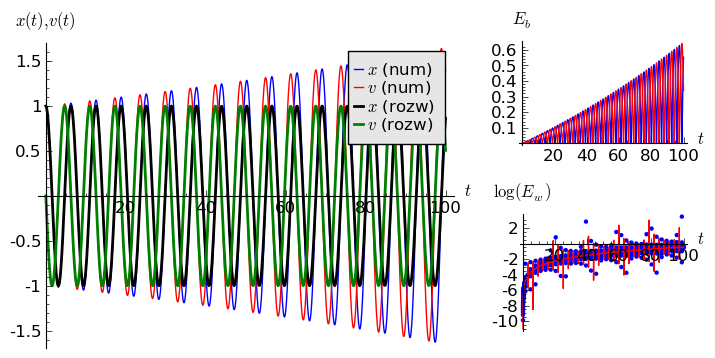
\includegraphics{euler_osc.png}
\caption{Porównanie numerycznego ($x(t)$ linia niebieska, $v(t)$ linia czerwona)
i analitycznego ($x(t)$ linia czarna, $v(t)$ linia zielona) rozwiązania zagadnienia
oscylatora harmonicznego. Jak widać odchylenia od rozwiązań dokładnych zaczynją być
znaczące już dla kilku kroków symulacji.
Błąd bezwzględny widnieje na prawym górny panelu; błąd względny wykreślony jest na prawym dolnym
panelu w skali logarytmicznej dla lepszej czytelności.
Parametry użyte dla powyższej symulacji: $x_0=1, v_0=0, \omega_0=1, h=0.01, N=10000$.}\end{figure}

Inną, aczkolwiek trudniejszą metodą będzie użycie algorytmów wyższego rzędu takich jak schemat Rungego-Kutty
(2-giego, 4-tego i wyższych rzędów). Dociekliwy student może zajrzeć
\href{http://en.wikipedia.org/wiki/List\_of\_Runge\%E2\%80\%93Kutta\_methods}{tutaj}.
\begin{description}
\item[{Zadanie D1.3}] \leavevmode
Przeprowadź podobną symulację dla innych wartości \emph{h}. Wykreśl zależność błędów względnego i bezwzględnego
w funkcji wartości \emph{h}. Błędy badaj po rzeczywistym czasie symulacji $T_E = 100$.

\item[{Zadanie D1.4}] \leavevmode
Rozwiązać numerycznie równania
\begin{enumerate}
\item {} 
$\dot{x} (t) = -k x^3$

\item {} 
$\dot{x} (t) = F$

\item {} 
$m \ddot{x} (t) = m g$

\item {} 
$\ddot{r} (t) = 4 \epsilon \left[ \left(\frac{\sigma}{r} \right)^{12}-  \left( \frac{\sigma}{r}\right)^6 \right]$, $r>0$

\item {} 
$m \ddot{x} (t) = -\gamma \dot{x}(t) - k x(t)$

\item {} 
$m \ddot{x} (t) =  -k x(t) -\gamma \dot{x}(t) + a \cos(\omega t)$

\end{enumerate}

Dla każdego przypadku (A-F) należy
\begin{enumerate}
\item {} 
narysować \emph{x} (dla D-F również \emph{v}) w funkcji \emph{t} (opisać osie),

\item {} 
odpowiedzieć na pytanie: z jakim ruchem mamy do czynienia {[}dla jakich parametrow równania ruch
jest cykliczny (periodyczny), dla jakich rozwiązanie jest stałe (niezmienne w czasie)...{]},

\item {} 
znaleźć błąd względny i bezwzględny, wykreślić w funkcji czasu.

\end{enumerate}

Pytania:
\begin{enumerate}
\item {} 
Czym różni się przypadek E od F?

\item {} 
Co opisuje potencjał w D? Jakie ma zastosowanie w fizyce?

\end{enumerate}

\end{description}


\section{Stochastyczne równania różniczkowe}
\label{ch5/chV013:stochastyczne-rownania-rozniczkowe}\label{ch5/chV013::doc}
Stochastyczne równania różniczkowe (SDE, od angielskiej nazwy Stochastic differential equations)
są obecnie uważane za standardowe narzędzie wykorzystywane do analizy niektórych wielkości opisujących
dynamikę rynków finansowych. Do tych wielkości należą ceny aktywów, stopy procentowe czy ich pochodne.
W przeciwieństwie do zwyczajnych równań różniczkowych, które posiadają jendoznaczne rozwiązanie,
rozwiązaniami SDE są ciągłe w czasie procesy stochastyczne. Metody komputerowe wykorzystywane do analizy
SDE bazują na klasycznych metodach wykorzystywanych do rozwiązywania tradycyjnych, deterministycznych
równań różniczkowych, są jednak uogólnione tak, aby radzić sobie z procesami losowymi.

Zestaw zmiennych losowych $X_t$ indeksowanych liczbami rzeczywistymi \emph{t} nazywamy procesem losowym
ciągłym (ze względu na czas). Każda \emph{realizacja} procesu losowego to przypadkowa wartość zmiennej
losowej $X_t$ dla każdego \emph{t}, jest więc funkcją czasu. Co ciekawe, \emph{każda} deterministyczna
funkcja $f(t)$ może być uważana za proces stochastyczny, którego wariancja znika.

Najbardziej znanym przykładem procesu losowego szeroko występującego w modelach fizyki, chemii ale i
rynków finansowych jest \emph{proces Wienera} $W(t) = W_t$, ciągły proces stochastyczny posiadający
nastepujące własności
\begin{enumerate}
\item {} 
jest to proces rzeczywisty,

\item {} 
startuje z zera ($W_0 = 0$),

\item {} 
ma stacjonarne i niezależne przyrosty na nieprzekrywających się przedziałach,

\item {} 
jest procesem Gaussa o zerowej wartości średniej $\langle W_t - W_s \rangle = 0$
i wariancji przyrostów $\langle [W_t - W_s]^2 \rangle = 2 D (t -s)$,

\item {} 
proces Wienera może być reprezentowany ciągłymi trajektoriami.

\end{enumerate}

Wynika z tego, że dla każdej różnicy czasów \emph{t - s} zmienna losowa $W_t - W_s$ jest zmienną losową
gaussowską o zerowej wartości średniej i wariancji $2D(t-s)$. Więc jego rozkład prawdopodobieństwa ma
postać
\begin{gather}
\begin{split}f_{W_t - W_s}(x) = \frac{1}{\sqrt{2 \pi D (t - s)}} \exp \Big[ -\frac{x^2}{4D(t-s)} \Big].\end{split}\notag
\end{gather}
Proces taki może być wyprowadzony jako proces graniczny błądzenia przypadkowego. Wystarczy tylko zbadać
granicę dla której wielkość skoku i czas pomiędzy skokami będą maleć do zera. Tak zdefiniowanym procesem
posługujemy się zwyczajowo, gdy podczas analizy probalmu pojawia się jakaś nieregularna siła czy zaburzenie
którego nie możemy opisać równaniami deterministycznymi.

Typowe dla rynków finansowych \emph{równanie dyfuzji} może być modelowane przez równanie różniczkowe posiadające
część deterministyczną zwaną \textbf{dryftem} oraz część losową zwaną \textbf{dyfuzją}. Ta ostatnia jest bardzo często
reprezentowana właśnie przez proces Wienera. Możemy sobie napisać ogólne równanie
\begin{gather}
\begin{split}dX = a(t, X) dt + b(t,X) dW_t.\end{split}\notag
\end{gather}
Jest to postać różniczkowa. W zwykłych równaniach różniczkowych zazwyczaj stosujemu pochodne $dx/dt$. W
tym przypadku postać różniczkowa ma większy sens, jako, że wiele interesujących nas procesów losowych (jak
ruch Browna) są procesami ciągłymi aczkolwiek nie są różniczkowalne. Powyższe równanie nabiera większego
sensu pod znakiem całki
\begin{gather}
\begin{split}X(t) = X(0) + \int_0^t a(s,y) ds \int_0^t b(s,y) dW_s.\end{split}\notag
\end{gather}
Ostatni wyraz z prawej zwany jest całką Ito.


\subsection{Równanie Blacka-Scholesa}
\label{ch5/chV013:rownanie-blacka-scholesa}
Jednym z bardziej znanych, historycznym już równaniem stochastycznym, jest równanie opisujące geometryczny
ruch Browna
\begin{gather}
\begin{split}dX = \mu X dt + \sigma X dW_t,\end{split}\notag
\end{gather}
gdzie $\mu, \sigma$ to wielkości stałe.
Równanie to jest jednym z podstawowych elementów modelu wyceny opcji Blacka-Scholesa. Teoria ta została
nagrodzona Nagrodą Nobla z ekonomii w roku 1997, a opracowana przez absolwenta fizyki i doktora matematyki
Fischera Blacka oraz ekonomistę Myrona Scholesa. Teoria Blacka-Scholesa pozwala na wycenę wartości tzw.
finansowych instrumentów pochodnych, czyli opcji, oraz służy do optymalizacji ``bezpiecznego'' portfela
inwestycyjnego.

Pomimo tego, że równanie to wygląda na proste, żeby nie powiedzieć zbyt proste na to by opisywać jakąkolwiek
rzeczywistość na rynkach finansowych, ma ono olbrzymie znaczenie, jako, że może być rozwiązane ściśle
dając wynikowy wzór z którego możemy wyliczyć zmianę cen prostych opcji. Jak już powiedzieliśmy,
rozwiązanie jest geometrycznym ruchem Browna
\begin{gather}
\begin{split}X(t) = X_0 \exp \Big[ \Big( \mu - \frac{\sigma^2}{2} \Big) t + \sigma dW_t \Big].\end{split}\notag
\end{gather}
Dzięki zamkniętej postaci rozwiązania mamy możliwość testowania metod numerycznych, które przedstawimy
poniżej.


\subsection{Schemat Eulera-Maruyamy}
\label{ch5/chV013:schemat-eulera-maruyamy}
Najprostszą metodą numerycznego rozwiązywania równań różniczkowych zwyczajnych jest metoda Eulera. Bazuje
ona np. na rozwinięciu Tylora w pierwszym rzędzie przybliżenia. Stochastycznym analogiem tej metody
jest metoda Eulera-Maruyamy.

Będziemy chcieli podać przybliżone rozwiązanie ogólnej postaci SDE na przedziale czasowym
$t \in [t_0,t_E]$. Na początku zdyskretyzujemy sobie ów przedział czasowy, ustalając na siatkę
\emph{N} punktów
\begin{gather}
\begin{split}t_0 < t_1 < t_2 < \dots < t_{N-2} < t_E.\end{split}\notag
\end{gather}
Dążymy do tego, aby na tej siatce znaleźć przybliżone wartości zmiennej $X$. Oznaczmy je
\begin{gather}
\begin{split}w_0 < w_1 < w_2< \dots < w_{N-2} < w_E.\end{split}\notag
\end{gather}
Są to oczywiście przybliżone rozwiązania zmiennej $x$ dla odpowiednich czasów z powyższej siatki
$\{t_i\}$. Zakładając wartość początkową dla SDE $X(t_0) = X_0$ możemy pokusić się
o rozwiązanie numeryczne w następującej postaci
\begin{gather}
\begin{split}w_0 = X_0\end{split}\notag\\\begin{split}w_{i+1} = w_i + a (t_i, w_i) \Delta t_{i+1} + b(t_i, w_i) \Delta W_{i+1}\end{split}\notag\\\begin{split}\Delta t_{i+1} = t_{i+1} - t_i\end{split}\notag\\\begin{split}\Delta W_{i+1} = W(t_{i+1}) - W(t_i).\end{split}\notag
\end{gather}
Kluczową sprawą w tym punkcie jest problem: jak zamodelować $\Delta W_i$? Mając do dyspozycji generator
liczb losowych z rozkładem \emph{N(0,1)} każdą losową liczbę $\Delta W_i$ obliczamy ze wzoru
\begin{gather}
\begin{split}\Delta W_i = \sqrt{\Delta t_i} z_i,\end{split}\notag
\end{gather}
gdzie $z_i$ jest losowana właśnie z \emph{N(0,1)}.
Aby scałkować proces stochastyczny użyjemy formuły na przyrost procesu Wienera
\begin{gather}
\begin{split}\int_{t_i}^{t_{i+1}} \Gamma(t) dt =
\int_{t_i}^{t_{i+1}} dW(t) =  W(t_{i+1}) - W(t_i)\end{split}\notag
\end{gather}
Z definicji procesu Wienera wiemy, że jest on procesem Gaussa o zerowej średniej i wariancji liniowej w czasie
$\langle [W(t_{i+1}) - W(t_i)]^2 \rangle = 2 D \Delta t_i$, co daje nam w sensie średnio-kwadratowym
$\Delta W \propto \sqrt{\langle [\Delta W (t)]^2 \rangle} = \sqrt{\Delta t_i}$. Scałkowanie procesu Wienera
prowadzi do
\begin{gather}
\begin{split}\int_{t_i}^{t_{i + 1}} dW_t = \sqrt{\Delta t_i} z_i.\end{split}\notag
\end{gather}
Jeżeli założymy sobie, że krok czasowy (odległości na siatce rozwiązań) jest stały i wynosi
$\Delta t_i = h$ możemy napisać schemat explicite
\begin{gather}
\begin{split}w_{i+1} = w_i + h a(t_i, w_i) + \sqrt{h} b(t_i, w_i) z_i.\end{split}\notag
\end{gather}
Jako, że każdy zestaw wartości $\{w_i\}, i=0,\dots,E$ wyprodukowany przez powyższą formułę
będzie przybliżonym rozwiązaniem procesu losowego, to i każda realizacja (każdy zestaw) będzie
również losowa, a co za tym idzie - każda realizacja procesu będzie inna.


\subsection{Schemat Millsteina}
\label{ch5/chV013:schemat-millsteina}
Dodaje on poprawkę do poprzedniego rozwiązania, powodując, że schemat staje się schematem pierwszego rzędu
w sensie silnym. Dany jest on wzorem iteracyjnym
\begin{gather}
\begin{split}w_0 = X_0\end{split}\notag\\\begin{split}w_{i+1} = w_i + a(w_i,t_i) h -
\frac{h}{2} b(x_i,t_i)\frac{\partial b}{\partial x}'(w_i,t_i)(z_i^2 - 1) +
\sqrt{h} b(w_i,t_i) z_i.\end{split}\notag
\end{gather}
Obie metody (Millsteina i Eulera-Maruyamy) redukują się do tego samego schematu gdy część losowa nie jest
zależna od zmiennej \emph{x}. Jeżeli zależność istnieje, schemat Millsteina będzie szybciej zbieżny od
schematu EM.


\section{Przykłady całkowania procesów stochastycznych}
\label{ch5/chV013:przyklady-calkowania-procesow-stochastycznych}

\subsection{Proces dyfuzji}
\label{ch5/chV013:proces-dyfuzji}
Jest to prawdopodobnie najprostszy proces stochastyczny wykorzystujący biały szum
gaussowski jako proces losowy. Przez matematyków nazywany jest po prostu procesem
Wienera ponieważ prawa strona równania ruchu zawiera tylko i wyłącznie ów proces.
Z drugiej strony jest obok procesu Poissona najważniejszym procesem losowym
na bazie którego można zdefiniować całą rodzinę procesów losowych o ciągłych
realizacjach. Równanie to można przedstawić używając równania Ito
\begin{gather}
\begin{split}d x(t) = \sqrt{2 D} dW(t).\end{split}\notag
\end{gather}
Realizacja jest funkcją ciągłą, ale nigdzie nieróżniczkowalną (jako że pochodna
procesu Wienera nie istnieje). Za pomocą znanego już schematu Eulera-Maruyamy (EM)
możemy sobie wygenerować pojedynczą realizację takiego procesu. Parametr $D$
reguluje natężenie szumu.
\begin{gather}
\begin{split}x_0 = 0\end{split}\notag\\\begin{split}x_{i+1} = x_i + \sqrt{2 h D} N(0,1).\end{split}\notag
\end{gather}
Wiemy, że dla
procesu Wienera $W(0) = 0$, wystartujemy więc z $x(0) = 0$. Weźmy
krok $h=0.01$ i 5000 kroków czasowych. Dla przejrzystości weźmiemy
natężenie szumu $D=1$. Jako, że wiemy jak generować zmienne z rozkładem
\emph{N(0,1)} użyjemy sobie ``symbolicznego'' oznaczenia na funkcję zwracajacą
takie zmienne. Funkcję taką nazwiemy \code{std\_norm}. Konkretna realizacja
takiej funkcji może odbywać np: poprzez algorytm Boxa-Mullera. Funkcja ta
będzie przy wywołaniu zwracała jedną liczbę losową z \emph{N(0,1)}.

\begin{Verbatim}[commandchars=\\\{\}]
\PYG{n}{h} \PYG{o}{=} \PYG{l+m+mf}{0.01}
\PYG{n}{N} \PYG{o}{=} \PYG{l+m+mi}{5000}
\PYG{n}{x0} \PYG{o}{=} \PYG{l+m+mi}{0}
\PYG{n}{D} \PYG{o}{=} \PYG{l+m+mi}{1}

\PYG{n}{x} \PYG{o}{=} \PYG{p}{[}\PYG{n}{x0}\PYG{p}{]}
\PYG{k}{for} \PYG{n}{i} \PYG{o+ow}{in} \PYG{n+nb}{xrange}\PYG{p}{(}\PYG{l+m+mi}{1}\PYG{p}{,}\PYG{n}{N}\PYG{p}{)}\PYG{p}{:}
  \PYG{n}{n01} \PYG{o}{=} \PYG{n}{std\PYGZus{}norm}\PYG{p}{(}\PYG{p}{)}
  \PYG{n}{x}\PYG{o}{.}\PYG{n}{append}\PYG{p}{(}\PYG{n}{x}\PYG{p}{[}\PYG{n}{i}\PYG{o}{\PYGZhy{}}\PYG{l+m+mi}{1}\PYG{p}{]} \PYG{o}{+} \PYG{n}{sqrt}\PYG{p}{(}\PYG{l+m+mi}{2}\PYG{o}{*}\PYG{n}{h}\PYG{o}{*}\PYG{n}{D}\PYG{p}{)} \PYG{o}{*} \PYG{n}{n01}\PYG{p}{)}
\end{Verbatim}

Teraz narysujmy sobie takie realizacje dla kilku różnych wartości parametru \emph{D}.
\begin{figure}[htbp]
\centering
\capstart

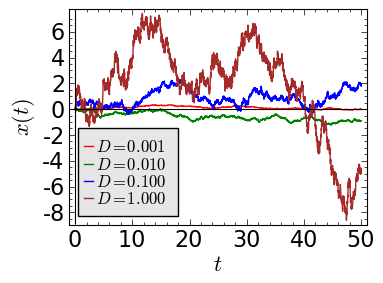
\includegraphics{dyf02.png}
\caption{Proces dyfuzji dla kilku różnych wartości parametru D.}\end{figure}

Na pierwszy rzut oka trajektorie (czy realizacje, przebiegi...) wyglądają kompletnie
inaczej. Dla małych wartości \emph{D} krzywe są bardziej regularne niż dla tych
parametryzowanych przez większe wartości \emph{D}, dla których to wykres jest mocno
poszarpany i nieregularny. Jeżeli jednak narysowalibyśmy je osobno, nie oznaczając
osi, identyfikacja byłaby niemożliwa - nie widzimy bowiem relacji pomiędzy
wartościami (przyrostami).
\begin{figure}[htbp]
\centering
\capstart

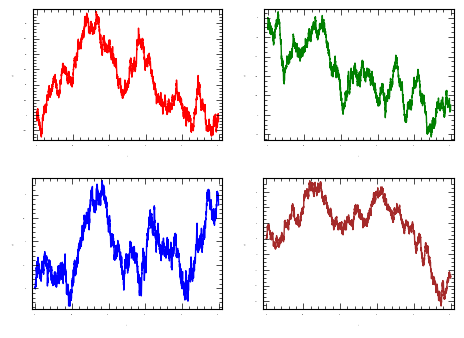
\includegraphics{dyf.png}
\caption{Proces dyfuzji dla kilku różnych wartości parametru D. Są to te same przebiegi co
w poprzednim wykresie. Kolory tu uzyte odpowiadają kolorom z wykresu poprzedniego.}\end{figure}

Jako, że rozwiązanie równania dyfuzji znane jest od dawoen dawna, możemy potestować
na ile dokładnie rozwiązujemy nasze równanie. Oczywiście jedyne co możemy określić,
to rozkład gęstości prawdopodobieństwa. Zakładając warunki początkowe
\begin{gather}
\begin{split}P(x,0) = \delta (x)\end{split}\notag
\end{gather}
co oznacza, że cały zespół cząstek podlegających dyfuzji wystartuje z $x(0)=0$,
możemy podać odpowiedź, bazując na równaniu dyfuzji
\begin{gather}
\begin{split}\frac{\partial P(x,t)}{\partial t} = D\frac{\partial^2 P(x,t)}{\partial x^2}.\end{split}\notag
\end{gather}
Wynikiem jest rozkład Gaussa postaci
\begin{gather}
\begin{split}P(x,t) = \frac{1}{\sqrt{4 \pi D t}} \exp \Big[ -\frac{x^2}{4 D t} \Big].\end{split}\notag
\end{gather}
w którym wariancja rośnie liniowo z czasem a średnia jest równa zero. Zobaczmy, czy jesteśmy w
stanie zweryfikować powyższy wzór numerycznie. Postaramy się znaleźć histogram
pozycji 10000 cząstek po 100 krokach i porównamy go z powyższym wynikiem. Założymy sobie
$D=0.1$ i krok czasowy $h=0.01$. Oznacza to, że po 100 krokach symulacji
osiągniemy rzeczywisty czas równy 1.
\begin{figure}[htbp]
\centering
\capstart

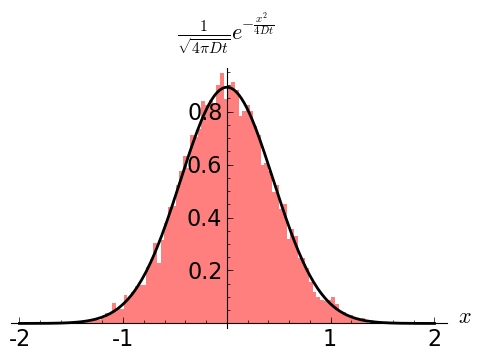
\includegraphics{dyf_100n.png}
\caption{Proces dyfuzji po 100 krokach symulacji dla $D=0.1$, $h=0.01$, $N=100$
a co za tym idzie $t=Nh$.}\end{figure}
\begin{description}
\item[{Zadanie 6.1.1}] \leavevmode
Wykonaj w Sage powyższy rysunek. Metodę generowania histogramów znajdziesz w pierwszej
części skryptu. Listę położeń, którą należy podać do histogramu wygeneruj w podobny
sposób jak na początku tego rozdziału.

\end{description}


\subsection{Dyfuzja ze stałym dryftem}
\label{ch5/chV013:dyfuzja-ze-stalym-dryftem}
Proces taki otrzymuje się bezpośrednio jako graniczny przypadek niesymetrycznego błądzenia
przypadkowego (polecam poczytać \href{http://el.us.edu.pl/ekonofizyka/index.php/PIZL:Proces\_Wienera\_i\_proces\_dyfuzji\#Przypadek\_niesymetryczny:\_dyfuzja\_z\_dryfem}{ten podrozdział}).
Równanie opisujące ten proces ma postać zbliżoną do poprzedniego, bogatsze jest jednak
o dodatkowy czynnik, zwany dryftem
\begin{gather}
\begin{split}\frac{\partial P(x,t)}{\partial t} = -V\frac{\partial P(x,t)}{\partial x} + D\frac{\partial^2 P(x,t)}{\partial x^2}.\end{split}\notag
\end{gather}
Rozwiązaniem równania dyfuzji z dryfem, z takim samym warunkiem początkowym jak poprzednio
(wszystkie cząstki, bądź realizacje zaczynają z tego samego położenia $x(0)=0$
jest następujaca funkcja
\begin{gather}
\begin{split}P(x,t) = \frac{1}{\sqrt{4 \pi D t}} \exp \Big[ -\frac{(x - Vt)^2}{4 D t} \Big].\end{split}\notag
\end{gather}
Jest to funkcja Gaussa opisujaca zmienne losowe normalne, a dwa pierwsze momenty wynoszą
odpowiednio $\xi(t) = Vt$ oraz $\sigma_{\xi}^2 = 2 D t$. Łatwo zauważyć, że
zarówno średnia jak i wariancja zależne są liniowo od czasu. Ponadto wariancja jest
identyczna jak w procesie dyfuzji bez dryftu. Dryft ów stały można z punktu widzenia fizyki
rozumieć jako stałą siłę przyłożoną do cząstki (coś na kształt cząstki umieszczonej na
równi pochyłej) - położenie cząstki rośnie liniowo z czasem (jak w ruchu jednostajnie
prostoliniowym), ale fluktuacje rosną w czasie jak pierwiastek $\sqrt{t}$.

Podobną analizę numeryczną jak poprzednio możemy przeprowadzić i tutaj. Tym razem, wykreślimy
sobie stroboskopowo histogram położeń po kilku krokach: \emph{N = 10, 100, 200}. Po lekkiej
modyfikacji numeryczny schemat EM będzie wyglądał tak

\begin{Verbatim}[commandchars=\\\{\}]
\PYG{n}{h} \PYG{o}{=} \PYG{l+m+mf}{0.01}
\PYG{n}{N} \PYG{o}{=} \PYG{l+m+mi}{5000}
\PYG{n}{x0} \PYG{o}{=} \PYG{l+m+mi}{0}
\PYG{n}{V} \PYG{o}{=} \PYG{l+m+mi}{1}
\PYG{n}{D} \PYG{o}{=} \PYG{l+m+mi}{1}

\PYG{n}{x} \PYG{o}{=} \PYG{p}{[}\PYG{n}{x0}\PYG{p}{]}
\PYG{k}{for} \PYG{n}{i} \PYG{o+ow}{in} \PYG{n+nb}{xrange}\PYG{p}{(}\PYG{l+m+mi}{1}\PYG{p}{,}\PYG{n}{N}\PYG{p}{)}\PYG{p}{:}
  \PYG{n}{n01} \PYG{o}{=} \PYG{n}{std\PYGZus{}norm}\PYG{p}{(}\PYG{p}{)}
  \PYG{n}{x}\PYG{o}{.}\PYG{n}{append}\PYG{p}{(}\PYG{n}{x}\PYG{p}{[}\PYG{n}{i}\PYG{o}{\PYGZhy{}}\PYG{l+m+mi}{1}\PYG{p}{]} \PYG{o}{+} \PYG{n}{V}\PYG{o}{*}\PYG{n}{h} \PYG{o}{+} \PYG{n}{sqrt}\PYG{p}{(}\PYG{l+m+mi}{2}\PYG{o}{*}\PYG{n}{h}\PYG{o}{*}\PYG{n}{D}\PYG{p}{)} \PYG{o}{*} \PYG{n}{n01}\PYG{p}{)}
\end{Verbatim}

Teraz wystarczy zobaczyć, czy histogramy położeń po czasie \emph{t=0.1, 1, 2} będą odpowiadały
obliczonej powyżej funkcji rozkładu.
\begin{figure}[htbp]
\centering
\capstart

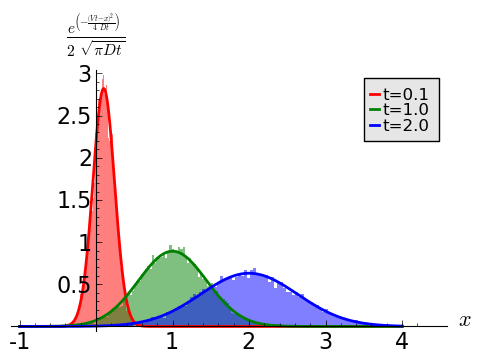
\includegraphics{dryftdif001.png}
\caption{Proces dyfuzji ze stałym dryftem po 10, 100 i 200 krokach symulacji dla $D=0.1$,
$h=0.01$, a co za tym idzie $t=0.1, 1, 2$.}\end{figure}

Możemy policzyć sobie teraz średnie, odchylenie standardowe oraz błędy względny i bezwzględny
przybliżeń dokładnych rozwiązań procesu dyfuzji z dryftem.

\begin{tabulary}{\linewidth}{|L|L|L|L|L|L|}
\hline
\textbf{
czas
} & \textbf{} & \textbf{
teoria
} & \textbf{
symulacje
} & \textbf{
$E_b$
} & \textbf{
$E_w$ {[}\%{]}
}\\\hline
 \multirow{2}{*}{
t=0.1
} & 
średnia
 & 
0.10
 & 
0.09972
 & 
0.0002766
 & 
0.2766
\\

std
 & 
0.1414
 & 
0.1413
 & 
0.00007544
 & 
0.05335
\\\hline
 \multirow{2}{*}{
t=1
} & 
średnia
 & 
1.0
 & 
1.005
 & 
0.005345
 & 
0.5345
\\

std
 & 
0.4472
 & 
0.444
 & 
0.003026
 & 
0.6766
\\\hline
 \multirow{2}{*}{
t=2
} & 
średnia
 & 
2.0
 & 
2.001
 & 
0.001460
 & 
0.07302
\\

std
 & 
0.6324
 & 
0.6362
 & 
0.003708
 & 
0.5863
\\\hline
\end{tabulary}


Jak widzimy błędy bezwzględne dochodzą do około pół punktu procentowego różnicy dla 10000
realizacji. Zwiekszenie próby spowoduje jeszcze lepsze dopasowanie, zmniejszenie spowoduje
większe odchylenia od wartości rzeczywistych.
\begin{description}
\item[{Zadanie 6.1.2}] \leavevmode
Oblicz błędy przybliżenia rozwiazania problemu dyfuzji ze stałym dryftem dla 10, 100, 500 i
1000 różnych realizacji. Zestawienia podaj w tabeli.

\end{description}


\subsection{Proces Ornsteina-Uhlenbecka}
\label{ch5/chV013:proces-ornsteina-uhlenbecka}

\subsection{Równanie Blacka-Scholesa}
\label{ch5/chV013:id1}

\section{Lapunov}
\label{ch5/chV014::doc}\label{ch5/chV014:lapunov}

\section{Bifurkacje}
\label{ch5/chV014:bifurkacje}

\section{ARMA}
\label{ch5/chV014:arma}
Analizując dane pochodzące z szeroko pojętych źródeł rynków finansowych dość często korzysta się z Modeli
Autoregresyjnych ze Średnią Kroczącą. Angielska nazwa takich modeli to Autoregresive Moving Average Models
i stąd nazwa ARMA. Zwykle procedura polega na pewnej analizie posiadanych danych i dopasowaniu
do nich parametrów takiego modelu. Takim zagadnieniem zajmuje się \href{http://el.us.edu.pl/ekonofizyka/index.php/Analiza\_Szeregów\_Czasowych}{Analiza Szeregów Czasowych}. Szeregów dostarcza ``samo życie'',
czyli np: giełda. Jako, że ten kurs ma na celu modelowanie rynków, czyli ma \emph{generować} takie szeregi,
pobawimy się teraz w symulowanie rynku.

Model ARMA to nic innego jak układ równań różnicowych ze stałymi współczynnikami.



\renewcommand{\indexname}{Indeks}
\printindex
\end{document}
